% Options for packages loaded elsewhere
\PassOptionsToPackage{unicode}{hyperref}
\PassOptionsToPackage{hyphens}{url}
%
\documentclass[
  12pt,
]{book}
\usepackage{amsmath,amssymb}
\usepackage{iftex}
\ifPDFTeX
  \usepackage[T1]{fontenc}
  \usepackage[utf8]{inputenc}
  \usepackage{textcomp} % provide euro and other symbols
\else % if luatex or xetex
  \usepackage{unicode-math} % this also loads fontspec
  \defaultfontfeatures{Scale=MatchLowercase}
  \defaultfontfeatures[\rmfamily]{Ligatures=TeX,Scale=1}
\fi
\usepackage{lmodern}
\ifPDFTeX\else
  % xetex/luatex font selection
\fi
% Use upquote if available, for straight quotes in verbatim environments
\IfFileExists{upquote.sty}{\usepackage{upquote}}{}
\IfFileExists{microtype.sty}{% use microtype if available
  \usepackage[]{microtype}
  \UseMicrotypeSet[protrusion]{basicmath} % disable protrusion for tt fonts
}{}
\makeatletter
\@ifundefined{KOMAClassName}{% if non-KOMA class
  \IfFileExists{parskip.sty}{%
    \usepackage{parskip}
  }{% else
    \setlength{\parindent}{0pt}
    \setlength{\parskip}{6pt plus 2pt minus 1pt}}
}{% if KOMA class
  \KOMAoptions{parskip=half}}
\makeatother
\usepackage{xcolor}
\usepackage{color}
\usepackage{fancyvrb}
\newcommand{\VerbBar}{|}
\newcommand{\VERB}{\Verb[commandchars=\\\{\}]}
\DefineVerbatimEnvironment{Highlighting}{Verbatim}{commandchars=\\\{\}}
% Add ',fontsize=\small' for more characters per line
\usepackage{framed}
\definecolor{shadecolor}{RGB}{248,248,248}
\newenvironment{Shaded}{\begin{snugshade}}{\end{snugshade}}
\newcommand{\AlertTok}[1]{\textcolor[rgb]{0.94,0.16,0.16}{#1}}
\newcommand{\AnnotationTok}[1]{\textcolor[rgb]{0.56,0.35,0.01}{\textbf{\textit{#1}}}}
\newcommand{\AttributeTok}[1]{\textcolor[rgb]{0.13,0.29,0.53}{#1}}
\newcommand{\BaseNTok}[1]{\textcolor[rgb]{0.00,0.00,0.81}{#1}}
\newcommand{\BuiltInTok}[1]{#1}
\newcommand{\CharTok}[1]{\textcolor[rgb]{0.31,0.60,0.02}{#1}}
\newcommand{\CommentTok}[1]{\textcolor[rgb]{0.56,0.35,0.01}{\textit{#1}}}
\newcommand{\CommentVarTok}[1]{\textcolor[rgb]{0.56,0.35,0.01}{\textbf{\textit{#1}}}}
\newcommand{\ConstantTok}[1]{\textcolor[rgb]{0.56,0.35,0.01}{#1}}
\newcommand{\ControlFlowTok}[1]{\textcolor[rgb]{0.13,0.29,0.53}{\textbf{#1}}}
\newcommand{\DataTypeTok}[1]{\textcolor[rgb]{0.13,0.29,0.53}{#1}}
\newcommand{\DecValTok}[1]{\textcolor[rgb]{0.00,0.00,0.81}{#1}}
\newcommand{\DocumentationTok}[1]{\textcolor[rgb]{0.56,0.35,0.01}{\textbf{\textit{#1}}}}
\newcommand{\ErrorTok}[1]{\textcolor[rgb]{0.64,0.00,0.00}{\textbf{#1}}}
\newcommand{\ExtensionTok}[1]{#1}
\newcommand{\FloatTok}[1]{\textcolor[rgb]{0.00,0.00,0.81}{#1}}
\newcommand{\FunctionTok}[1]{\textcolor[rgb]{0.13,0.29,0.53}{\textbf{#1}}}
\newcommand{\ImportTok}[1]{#1}
\newcommand{\InformationTok}[1]{\textcolor[rgb]{0.56,0.35,0.01}{\textbf{\textit{#1}}}}
\newcommand{\KeywordTok}[1]{\textcolor[rgb]{0.13,0.29,0.53}{\textbf{#1}}}
\newcommand{\NormalTok}[1]{#1}
\newcommand{\OperatorTok}[1]{\textcolor[rgb]{0.81,0.36,0.00}{\textbf{#1}}}
\newcommand{\OtherTok}[1]{\textcolor[rgb]{0.56,0.35,0.01}{#1}}
\newcommand{\PreprocessorTok}[1]{\textcolor[rgb]{0.56,0.35,0.01}{\textit{#1}}}
\newcommand{\RegionMarkerTok}[1]{#1}
\newcommand{\SpecialCharTok}[1]{\textcolor[rgb]{0.81,0.36,0.00}{\textbf{#1}}}
\newcommand{\SpecialStringTok}[1]{\textcolor[rgb]{0.31,0.60,0.02}{#1}}
\newcommand{\StringTok}[1]{\textcolor[rgb]{0.31,0.60,0.02}{#1}}
\newcommand{\VariableTok}[1]{\textcolor[rgb]{0.00,0.00,0.00}{#1}}
\newcommand{\VerbatimStringTok}[1]{\textcolor[rgb]{0.31,0.60,0.02}{#1}}
\newcommand{\WarningTok}[1]{\textcolor[rgb]{0.56,0.35,0.01}{\textbf{\textit{#1}}}}
\usepackage{longtable,booktabs,array}
\usepackage{calc} % for calculating minipage widths
% Correct order of tables after \paragraph or \subparagraph
\usepackage{etoolbox}
\makeatletter
\patchcmd\longtable{\par}{\if@noskipsec\mbox{}\fi\par}{}{}
\makeatother
% Allow footnotes in longtable head/foot
\IfFileExists{footnotehyper.sty}{\usepackage{footnotehyper}}{\usepackage{footnote}}
\makesavenoteenv{longtable}
\usepackage{graphicx}
\makeatletter
\newsavebox\pandoc@box
\newcommand*\pandocbounded[1]{% scales image to fit in text height/width
  \sbox\pandoc@box{#1}%
  \Gscale@div\@tempa{\textheight}{\dimexpr\ht\pandoc@box+\dp\pandoc@box\relax}%
  \Gscale@div\@tempb{\linewidth}{\wd\pandoc@box}%
  \ifdim\@tempb\p@<\@tempa\p@\let\@tempa\@tempb\fi% select the smaller of both
  \ifdim\@tempa\p@<\p@\scalebox{\@tempa}{\usebox\pandoc@box}%
  \else\usebox{\pandoc@box}%
  \fi%
}
% Set default figure placement to htbp
\def\fps@figure{htbp}
\makeatother
\setlength{\emergencystretch}{3em} % prevent overfull lines
\providecommand{\tightlist}{%
  \setlength{\itemsep}{0pt}\setlength{\parskip}{0pt}}
\setcounter{secnumdepth}{5}
\usepackage{booktabs}
\usepackage{amsthm}
\makeatletter
\def\thm@space@setup{%
  \thm@preskip=8pt plus 2pt minus 4pt
  \thm@postskip=\thm@preskip
}
\makeatother


%\usepackage[legalpaper, margin=1in]{geometry}

\usepackage[a4paper, total={6.5in, 9in}]{geometry}

\usepackage[]{natbib}
\bibliographystyle{apalike}
\usepackage{bookmark}
\IfFileExists{xurl.sty}{\usepackage{xurl}}{} % add URL line breaks if available
\urlstyle{same}
\hypersetup{
  pdftitle={The Identification of Dynamic Structural Shocks},
  pdfauthor={Kenza Benhima and Jean-Paul Renne},
  hidelinks,
  pdfcreator={LaTeX via pandoc}}

\title{The Identification of Dynamic Structural Shocks}
\author{Kenza Benhima and Jean-Paul Renne}
\date{2025-11-01}

\usepackage{amsthm}
\newtheorem{theorem}{Theorem}[chapter]
\newtheorem{lemma}{Lemma}[chapter]
\newtheorem{corollary}{Corollary}[chapter]
\newtheorem{proposition}{Proposition}[chapter]
\newtheorem{conjecture}{Conjecture}[chapter]
\theoremstyle{definition}
\newtheorem{definition}{Definition}[chapter]
\theoremstyle{definition}
\newtheorem{example}{Example}[chapter]
\theoremstyle{definition}
\newtheorem{exercise}{Exercise}[chapter]
\theoremstyle{definition}
\newtheorem{hypothesis}{Hypothesis}[chapter]
\theoremstyle{remark}
\newtheorem*{remark}{Remark}
\newtheorem*{solution}{Solution}
\begin{document}
\maketitle

{
\setcounter{tocdepth}{1}
\tableofcontents
}
\newcommand{\bv}[1]{\mathbf{#1}}

\chapter*{The Identification of Dynamic Structural Shocks}\label{intro}

The identification and estimation of dynamic responses to structural shocks is one of the principal goals of macroeconometrics. These responses correspond to the effect, over time, of an exogenous intervention that propagates through the economy, as modeled by a system of simultaneous equations.

Over the last decades, several methodologies have been proposed so as to estimate these responses. The objective of this course, developed by \href{https://sites.google.com/site/benhimakenza/}{Kenza Benhima} and \href{https://www.jprenne.com}{Jean-Paul Renne}, is to provide an exhaustive view of these methodologies and to provide students with tools enabling them to implement them in various contexts.

Codes associated with this course are part of the \texttt{IdSS} package (\textbf{Id}entification of \textbf{S}tructural \textbf{S}hocks), which is available on GitHub. To load a package from GitHub, you need to use function \texttt{install\_github} from the \texttt{devtools} package:

\begin{Shaded}
\begin{Highlighting}[]
\FunctionTok{install.packages}\NormalTok{(}\StringTok{"devtools"}\NormalTok{) }\CommentTok{\# devtools allows to use "install\_github"}
\FunctionTok{library}\NormalTok{(devtools)}
\FunctionTok{install\_github}\NormalTok{(}\StringTok{"jrenne/IdSS"}\NormalTok{)}
\FunctionTok{library}\NormalTok{(IdSS)}
\end{Highlighting}
\end{Shaded}

\textbf{Useful (R) links:}

\begin{itemize}
\item
  Download R:

  \begin{itemize}
  \tightlist
  \item
    R software: \url{https://cran.r-project.org} (the basic R software)
  \item
    RStudio: \url{https://www.rstudio.com} (a convenient R editor)
  \end{itemize}
\item
  Tutorials:

  \begin{itemize}
  \tightlist
  \item
    Rstudio: \url{https://dss.princeton.edu/training/RStudio101.pdf} (by Oscar Torres-Reyna)
  \item
    R: \url{https://cran.r-project.org/doc/contrib/Paradis-rdebuts_en.pdf} (by Emmanuel Paradis)
  \item
    Our own tutorial: \url{https://jrenne.shinyapps.io/Rtuto_publiShiny/}
  \end{itemize}
\end{itemize}

\chapter{VARs and IRFs: the basics}\label{basics}

Often, impulse response functions (IRFs) are generated in the context of vectorial autoregressive (VAR) models. This section presents these models and show how they can be used to compute IRFs.

\section{Definition of VARs (and SVARMA) models}\label{definition-of-vars-and-svarma-models}

\begin{definition}[(S)VAR model]
\protect\hypertarget{def:SVAR}{}\label{def:SVAR}Let \(y_{t}\) denote a \(n \times1\) vector of (endogenous) random variables. Process \(y_{t}\) follows a \(p^{th}\)-order (S)VAR if, for all \(t\), we have
\begin{eqnarray}
\begin{array}{rllll}
VAR:& y_t &=& c + \Phi_1 y_{t-1} + \dots + \Phi_p y_{t-p} + \varepsilon_t,\\
SVAR:& y_t &=& c + \Phi_1 y_{t-1} + \dots + \Phi_p y_{t-p} + B \eta_t,
\end{array}
\label{eq:yVAR}
\end{eqnarray}
with \(\varepsilon_t = B\eta_t\), where \(\{\eta_{t}\}\) is a white noise sequence whose components are mutually and serially independent, and that satisfies \(\mathbb{V}ar(\eta_t)=Id\).
\end{definition}

The first line of Eq. \eqref{eq:yVAR} corresponds to the \textbf{reduced-form} of the VAR model (\textbf{structural form} for the second line). While the \textbf{structural shocks} (the components of \(\eta_t\)) are mutually uncorrelated, this is not the case of the \textbf{innovations}, that are the components of \(\varepsilon_t\). However, in both cases, vectors \(\eta_t\) and \(\varepsilon_t\) are serially uncorrelated (through time).

Notice that \(\mathbb{V}ar(\eta_t)=Id\) and \(\varepsilon_t = B\eta_t\) jointly imply that \[
\Omega :=\mathbb{V}ar(\varepsilon_t)=\mathbb{V}ar(B\eta_t)= B  \mathbb{V}ar(\eta_t) B'=BB'.
\]

Eq. \eqref{eq:yVAR} can also be rewritten using the lag operator \(L\), which gives:\footnote{The lag operator \(L\) transforms a process into a lagged process; e.g., \(L y_t = y_{t-1}\), and \(L^k y_t = y_{t-k}\), where \(k \in \mathbb{N}\).}
\[
y_t = c + \Phi(L) y_{t} + \varepsilon_t,
\]
where \(\Phi(L)=\Phi_1 L + \dots + \Phi_p L^p\).

As is the case for univariate models, VARs can be extended with MA terms in \(\eta_t\), giving rise to VARMA models:

\begin{definition}[(S)VARMA model]
\protect\hypertarget{def:SVARMA}{}\label{def:SVARMA}Let \(y_{t}\) denote a \(n \times1\) vector of random variables. Process \(y_{t}\) follows a VARMA model of order (p,q) if, for all \(t\), we have
\begin{eqnarray}
\begin{array}{rllll}
VARMA:& y_t &=& c + \Phi_1 y_{t-1} + \dots + \Phi_p y_{t-p} + \\
&&&\varepsilon_t + \Theta_1\varepsilon_{t-1} + \dots + \Theta_q \varepsilon_{t-q},\\
SVARMA:& y_t &=& c + \Phi_1 y_{t-1} + \dots + \Phi_p y_{t-p} + \\
&&& B_0 \eta_t + B_1 \eta_{t-1} + \dots +  B_q \eta_{t-q},
\end{array}
\label{eq:yVARMA}
\end{eqnarray}
with \(\varepsilon_t = B_0\eta_t\), and \(B_j = \Theta_j B_0\), for \(j \ge 0\) (with \(\Theta_0=Id\)), where \(\{\eta_{t}\}\) is a white noise sequence whose components are are mutually and serially independent.
\end{definition}

\section{IRFs in SVARMA}\label{IRFSVARMA}

One of the main objectives of macro-econometrics is to derive IRFs, that represent the dynamic effects of structural shocks (components of \(\eta_t\)) though the system of variables \(y_t\).

Formally, an IRF is a difference in conditional expectations:
\begin{equation}
\boxed{\Psi_{i,j,h} = \mathbb{E}(y_{i,t+h}|\eta_{j,t}=1) - \mathbb{E}(y_{i,t+h})}
\label{eq:boxIRFs}
\end{equation}
(effect on \(y_{i,t+h}\) of a one-unit shock on \(\eta_{j,t}\)).

IRFs closely relate to the Wold decomposition of \(y_t\). Indeed, if the dynamics of process \(y_t\) can be described as a VARMA model (which includes the case of VAR models), and if \(y_t\) is covariance stationary (see Def. \ref{def:covstat}), then \(y_t\) admits the following infinite MA representation (or Wold decomposition):
\begin{equation}
\boxed{y_t = \mu + \sum_{i=0}^\infty \Psi_{i} \eta_{t-i}.}
\label{eq:InfMA}
\end{equation}
or, shifted by \(h\) periods:
\begin{eqnarray*}
y_{t+h} &=& \mu + \sum_{i=0}^\infty \Psi_{i} \eta_{t+h-i}\\
&=& \mu + \underbrace{\sum_{i=0}^{h-1} \Psi_{i} \eta_{t+h-i}}_{\mbox{Effect of }\eta_{t+1},\dots,\eta_{t+h}} + \underbrace{\Psi_{h} \eta_{t}}_{\mbox{Effect of }\eta_{t}} + \underbrace{\sum_{i=h+1}^\infty \Psi_{i} \eta_{t+h-i}}_{\mbox{Effect of }\eta_{t-1},\eta_{t-2,\dots}}.
\end{eqnarray*}

With these notations, we get \(\mathbb{E}(y_{i,t+h}|\eta_{j,t}=1) = \mu_i + \Psi_{i,j,h}\), where \(\Psi_{i,j,h}\) is the component \((i,j)\) of matrix \(\Psi_h\) and \(\mu_i\) is the \(i^{th}\) entry of vector \(\mu\). Since we also have \(\mathbb{E}(y_{i,t+h})=\mu_i\), we obtain Eq. \eqref{eq:boxIRFs}.

\begin{example}[IRF of a univariate AR model]
\protect\hypertarget{exm:IRFsimpleAR}{}\label{exm:IRFsimpleAR}

To fix ideas, consider a simple univariate AR(1) process:
\[
y_t = \phi y_{t-1} + b \eta_t, \quad \eta_t \sim \text{i.i.d. }\mathcal{N}(0,1).
\]

We assume \(|\phi| < 1\) so that the process is covariance stationary.

Iterating forward:
\[
y_{t+h} = b \eta_{t+h} + \phi b \eta_{t+h-1} + \dots + \phi^h b \eta_t + \phi^{h+1} y_{t-1}.
\]
If the \(\eta_t\)'s are independent, we have \(\mathbb{E}(\eta_{t+h}|\eta_t = 1)=0\) if \(h \ne 0\) (and 1 otherwise). Therefore:
\[
\mathbb{E}(y_{t+h}|\eta_t = 1) - \mathbb{E}(y_{t+h}) = \phi^h b.
\]
Hence, the \textbf{impulse response function (IRF)} at horizon \(h\) is simply \$\Psi\_h = \phi\^{}h b \$.

\begin{Shaded}
\begin{Highlighting}[]
\NormalTok{phi }\OtherTok{\textless{}{-}}\NormalTok{ .}\DecValTok{8}
\NormalTok{b }\OtherTok{\textless{}{-}}\NormalTok{ .}\DecValTok{5}
\FunctionTok{plot}\NormalTok{(phi}\SpecialCharTok{\^{}}\NormalTok{(}\DecValTok{0}\SpecialCharTok{:}\DecValTok{30}\NormalTok{)}\SpecialCharTok{*}\NormalTok{b,}\AttributeTok{type=}\StringTok{"b"}\NormalTok{,}\AttributeTok{lwd=}\DecValTok{2}\NormalTok{,}\AttributeTok{xlab=}\StringTok{"Periods after shock"}\NormalTok{,}\AttributeTok{ylab=}\StringTok{""}\NormalTok{,}\AttributeTok{las=}\DecValTok{1}\NormalTok{)}
\FunctionTok{grid}\NormalTok{()}
\end{Highlighting}
\end{Shaded}

\begin{figure}
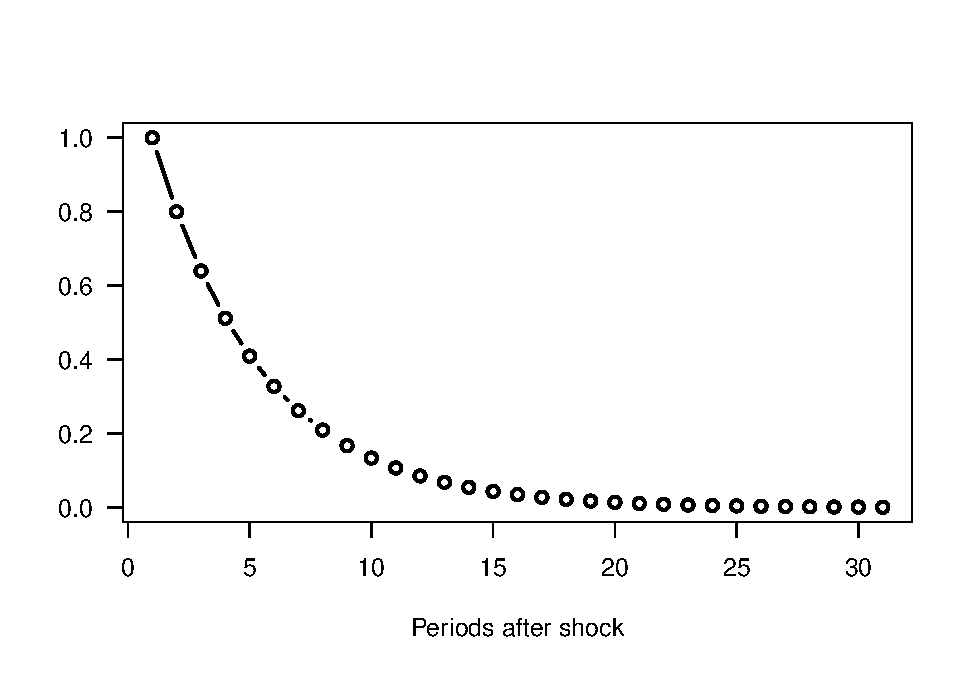
\includegraphics[width=0.9\linewidth]{IdentifStructShocks_files/figure-latex/simAR1-1} \caption{Impulse response functions for an AR(1) process: $y_t = \phi y_{t-1} + b \eta_t$, $\eta_t \sim i.i.d. \mathcal{N}(0,1)$.}\label{fig:simAR1}
\end{figure}

\end{example}

Hence, estimating IRFs amounts to estimating the \(\Psi_h\) matrices. In practice, three main approaches are commonly used:

\begin{itemize}
\item
  Calibrate and solve a (purely structural) Dynamic Stochastic General Equilibrium (DSGE) model at first order (linear approximation). The resulting solution can be written in the form of Eq. \eqref{eq:InfMA}.
\item
  Directly estimate the \(\Psi_h\) matrices using \textbf{projection methods} (see Section \ref{Projections}).
\item
  Approximate the infinite moving-average representation by estimating a parsimonious model, such as a \textbf{VAR(MA)} model (see Section \ref{estimVAR}). Once a (structural) VARMA representation is obtained, Eq. \eqref{eq:InfMA} follows immediately from the result stated in the next proposition.
\end{itemize}

\begin{proposition}[IRF of an ARMA(p,q) process]
\protect\hypertarget{prp:computPsi}{}\label{prp:computPsi}

If \(y_t\) follows the VARMA model described in Def. \ref{def:SVARMA}, then the matrices \(\Psi_h\) appearing in Eq. \eqref{eq:InfMA} can be computed recursively as follows:

\begin{enumerate}
\def\labelenumi{\arabic{enumi}.}
\tightlist
\item
  Set \(\Psi_{-1}=\dots=\Psi_{-p}=0\).
\item
  For \(h \ge 0\), (recursively) apply:
  \[
  \Psi_h = \Phi_1 \Psi_{h-1} + \dots + \Phi_p \Psi_{h-p} + \Theta_h B_0,
  \]
  with \(\Theta_0 = Id\) and \(\Theta_h = 0\) for \(h>q\).
\end{enumerate}

\end{proposition}

\begin{proof}
This is obtained by applying the operator \(\frac{\partial}{\partial \eta_{t}}\) on both sides of Eq. \eqref{eq:yVARMA}.
\end{proof}

Typically, consider the VAR(2) case. The first steps of the algorithm mentioned in the last bullet point are as follows:
\begin{eqnarray*}
y_t &=& \Phi_1 {\color{blue}y_{t-1}} + \Phi_2 y_{t-2} + B \eta_t  \\
&=& \Phi_1 \color{blue}{(\Phi_1 y_{t-2} + \Phi_2 y_{t-3} + B \eta_{t-1})} + \Phi_2 y_{t-2} + B \eta_t  \\
&=& B \eta_t + \Phi_1 B \eta_{t-1} + (\Phi_2 + \Phi_1^2) \color{red}{y_{t-2}} + \Phi_1\Phi_2 y_{t-3}  \\
&=& B \eta_t + \Phi_1 B \eta_{t-1} + (\Phi_2 + \Phi_1^2) \color{red}{(\Phi_1 y_{t-3} + \Phi_2 y_{t-4} + B \eta_{t-2})} + \Phi_1\Phi_2 y_{t-3} \\
&=& \underbrace{B}_{=\Psi_0} \eta_t + \underbrace{\Phi_1 B}_{=\Psi_1} \eta_{t-1} + \underbrace{(\Phi_2 + \Phi_1^2)B}_{=\Psi_2} \eta_{t-2} + f(y_{t-3},y_{t-4}).
\end{eqnarray*}

In particular, we have \(B = \Psi_0\). Matrix \(B\) indeed captures the contemporaneous impact of \(\eta_t\) on \(y_t\). That is why matrix \(B\) is sometimes called \textbf{impulse matrix}.

\begin{example}[IRFs of an SVAR model]
\protect\hypertarget{exm:IRFVAR}{}\label{exm:IRFVAR}

Consider the following VAR(2) model:
\begin{eqnarray}
\quad y_t &=&
\underbrace{\left[\begin{array}{cc}
0.6 & 0.2 \\
0 & 0.5
\end{array}\right]}_{=\Phi_1}
y_{t-1} +  
\underbrace{\left[\begin{array}{cc}
-0.1 & 0.1 \\
0.2 & 0.3
\end{array}\right]}_{=\Phi_2}y_{t-2} + \underbrace{\left[\begin{array}{cc}
0.5 & 1.5 \\
-1 & 0.8
\end{array}\right]}_{=B} \eta_{t}.
\label{eq:VAR111}
\end{eqnarray}

We can use function \texttt{simul.VARMA} of package \texttt{IdSS} to produce IRFs (using \texttt{indic.IRF=1} in the list of arguments):

\begin{Shaded}
\begin{Highlighting}[]
\FunctionTok{library}\NormalTok{(IdSS)}
\CommentTok{\# {-}{-}{-}{-} Specify model: {-}{-}{-}{-}}
\NormalTok{Phi }\OtherTok{\textless{}{-}} \FunctionTok{array}\NormalTok{(}\ConstantTok{NaN}\NormalTok{,}\FunctionTok{c}\NormalTok{(}\DecValTok{2}\NormalTok{,}\DecValTok{2}\NormalTok{,}\DecValTok{2}\NormalTok{)) }\CommentTok{\# (2,2,2) for (n,n,p)}
\NormalTok{Phi[,,}\DecValTok{1}\NormalTok{] }\OtherTok{\textless{}{-}} \FunctionTok{matrix}\NormalTok{(}\FunctionTok{c}\NormalTok{(.}\DecValTok{6}\NormalTok{,}\DecValTok{0}\NormalTok{,.}\DecValTok{2}\NormalTok{,.}\DecValTok{5}\NormalTok{),}\DecValTok{2}\NormalTok{,}\DecValTok{2}\NormalTok{)}
\NormalTok{Phi[,,}\DecValTok{2}\NormalTok{] }\OtherTok{\textless{}{-}} \FunctionTok{matrix}\NormalTok{(}\FunctionTok{c}\NormalTok{(}\SpecialCharTok{{-}}\NormalTok{.}\DecValTok{1}\NormalTok{,.}\DecValTok{2}\NormalTok{,.}\DecValTok{1}\NormalTok{,.}\DecValTok{3}\NormalTok{),}\DecValTok{2}\NormalTok{,}\DecValTok{2}\NormalTok{)}
\NormalTok{c }\OtherTok{\textless{}{-}} \FunctionTok{c}\NormalTok{(}\DecValTok{1}\NormalTok{,}\DecValTok{2}\NormalTok{)}
\NormalTok{B }\OtherTok{\textless{}{-}} \FunctionTok{matrix}\NormalTok{(}\FunctionTok{c}\NormalTok{(.}\DecValTok{5}\NormalTok{,}\SpecialCharTok{{-}}\DecValTok{1}\NormalTok{,}\FloatTok{1.5}\NormalTok{,.}\DecValTok{8}\NormalTok{),}\DecValTok{2}\NormalTok{,}\DecValTok{2}\NormalTok{)}
\NormalTok{Model }\OtherTok{\textless{}{-}} \FunctionTok{list}\NormalTok{(}\AttributeTok{c =}\NormalTok{ c,}\AttributeTok{Phi =}\NormalTok{ Phi,}\AttributeTok{B =}\NormalTok{ B)}
\CommentTok{\# {-}{-}{-}{-} Define first shock: {-}{-}{-}{-}}
\NormalTok{eta0 }\OtherTok{\textless{}{-}} \FunctionTok{c}\NormalTok{(}\DecValTok{1}\NormalTok{,}\DecValTok{0}\NormalTok{)}
\NormalTok{res.sim}\FloatTok{.1} \OtherTok{\textless{}{-}} \FunctionTok{simul.VARMA}\NormalTok{(Model,}\AttributeTok{nb.sim=}\DecValTok{30}\NormalTok{,}\AttributeTok{eta0=}\NormalTok{eta0,}\AttributeTok{indic.IRF=}\DecValTok{1}\NormalTok{)}
\CommentTok{\# {-}{-}{-}{-} Define second shock: {-}{-}{-}{-}}
\NormalTok{eta0 }\OtherTok{\textless{}{-}} \FunctionTok{c}\NormalTok{(}\DecValTok{0}\NormalTok{,}\DecValTok{1}\NormalTok{)}
\NormalTok{res.sim}\FloatTok{.2} \OtherTok{\textless{}{-}} \FunctionTok{simul.VARMA}\NormalTok{(Model,}\AttributeTok{nb.sim=}\DecValTok{30}\NormalTok{,}\AttributeTok{eta0=}\NormalTok{eta0,}\AttributeTok{indic.IRF=}\DecValTok{1}\NormalTok{)}
\CommentTok{\# {-}{-}{-}{-} Prepare plots: {-}{-}{-}{-}}
\FunctionTok{par}\NormalTok{(}\AttributeTok{plt=}\FunctionTok{c}\NormalTok{(.}\DecValTok{15}\NormalTok{,.}\DecValTok{95}\NormalTok{,.}\DecValTok{25}\NormalTok{,.}\DecValTok{8}\NormalTok{)) }\CommentTok{\# define margins}
\FunctionTok{par}\NormalTok{(}\AttributeTok{mfrow=}\FunctionTok{c}\NormalTok{(}\DecValTok{2}\NormalTok{,}\DecValTok{2}\NormalTok{)) }\CommentTok{\# 2 rows and 2 columns of plots}
\ControlFlowTok{for}\NormalTok{(i }\ControlFlowTok{in} \DecValTok{1}\SpecialCharTok{:}\DecValTok{2}\NormalTok{)\{}
  \ControlFlowTok{if}\NormalTok{(i }\SpecialCharTok{==} \DecValTok{1}\NormalTok{)\{res.sim }\OtherTok{\textless{}{-}}\NormalTok{ res.sim}\FloatTok{.1}\NormalTok{\}}\ControlFlowTok{else}\NormalTok{\{res.sim }\OtherTok{\textless{}{-}}\NormalTok{ res.sim}\FloatTok{.2}\NormalTok{\}}
  \ControlFlowTok{for}\NormalTok{(j }\ControlFlowTok{in} \DecValTok{1}\SpecialCharTok{:}\DecValTok{2}\NormalTok{)\{}
    \FunctionTok{plot}\NormalTok{(res.sim}\SpecialCharTok{$}\NormalTok{Y[j,],}\AttributeTok{las=}\DecValTok{1}\NormalTok{,}
         \AttributeTok{type=}\StringTok{"l"}\NormalTok{,}\AttributeTok{lwd=}\DecValTok{3}\NormalTok{,}\AttributeTok{xlab=}\StringTok{""}\NormalTok{,}\AttributeTok{ylab=}\StringTok{""}\NormalTok{,}
         \AttributeTok{main=}\FunctionTok{paste}\NormalTok{(}\StringTok{"Resp. of y"}\NormalTok{,j,}
                    \StringTok{" to a 1{-}unit increase in η"}\NormalTok{,i,}\AttributeTok{sep=}\StringTok{""}\NormalTok{))}
    \FunctionTok{abline}\NormalTok{(}\AttributeTok{h=}\DecValTok{0}\NormalTok{,}\AttributeTok{col=}\StringTok{"grey"}\NormalTok{,}\AttributeTok{lty=}\DecValTok{3}\NormalTok{)}
\NormalTok{  \}\}}
\end{Highlighting}
\end{Shaded}

\begin{figure}
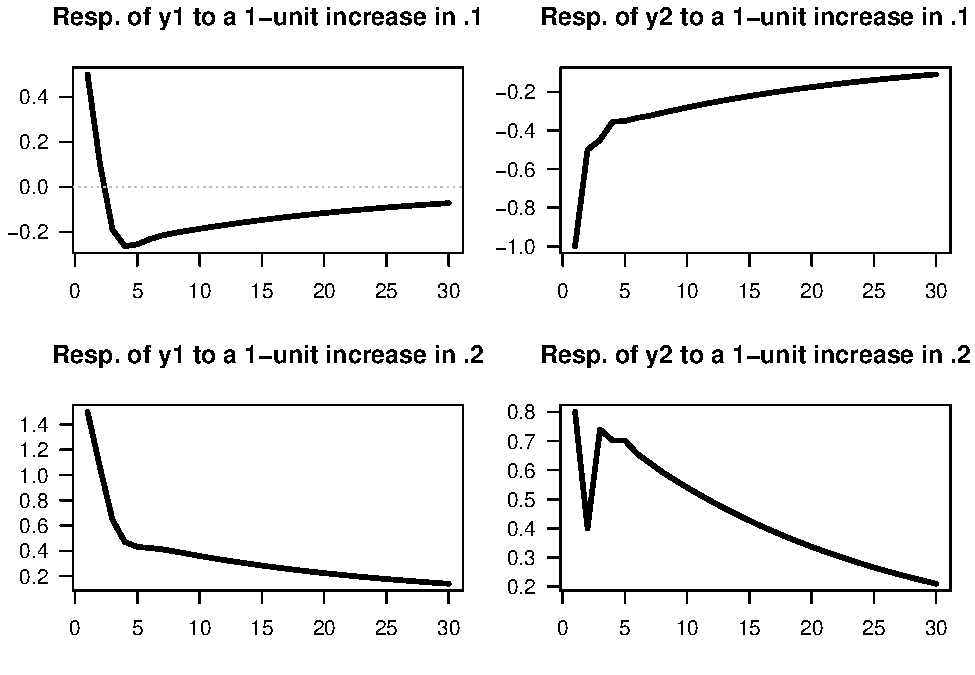
\includegraphics[width=0.95\linewidth]{IdentifStructShocks_files/figure-latex/simVAR2-1} \caption{Impulse response functions (VAR(2) specified above).}\label{fig:simVAR2}
\end{figure}

The same type of output would be obtained by using the function \texttt{simul.VAR} of package \texttt{IdSS}:\footnote{In that case, \texttt{res.sim} is of dimension \texttt{nb.sim}\(\times n\).}

\begin{Shaded}
\begin{Highlighting}[]
\NormalTok{res.sim }\OtherTok{\textless{}{-}} \FunctionTok{simul.VAR}\NormalTok{(}\AttributeTok{c=}\NormalTok{c,}\AttributeTok{Phi=}\NormalTok{Phi,}\AttributeTok{B=}\NormalTok{B,}\AttributeTok{nb.sim=}\DecValTok{30}\NormalTok{,}\AttributeTok{indic.IRF=}\DecValTok{1}\NormalTok{,}\AttributeTok{u.shock=}\NormalTok{eta0)}
\end{Highlighting}
\end{Shaded}

\end{example}

\begin{example}[IRFs of an SVARMA model]
\protect\hypertarget{exm:IRFVARMA}{}\label{exm:IRFVARMA}

Consider the following VARMA(1,1) model:
\begin{eqnarray}
\quad y_t &=&
\underbrace{\left[\begin{array}{cc}
0.5 & 0.3 \\
-0.4 & 0.7
\end{array}\right]}_{\Phi_1}
y_{t-1} +  \\
&& \underbrace{\left[\begin{array}{cc}
1 & 2 \\
-1 & 1
\end{array}\right]}_{B}\eta_t + \underbrace{\left[\begin{array}{cc}
0.4 & 0 \\
-1 & -0.5
\end{array}\right]}_{\Theta_1} \underbrace{\left[\begin{array}{cc}
1 & 2 \\
-1 & 1
\end{array}\right]}_{B}\eta_{t-1}.
\label{eq:VARMA111}
\end{eqnarray}

We can use function \texttt{simul.VARMA} of package \texttt{IdSS} to produce IRFs (using \texttt{indic.IRF=1} in the list of arguments):

\begin{Shaded}
\begin{Highlighting}[]
\FunctionTok{library}\NormalTok{(IdSS)}
\CommentTok{\# {-}{-}{-}{-} Specify model: {-}{-}{-}{-}}
\NormalTok{Phi }\OtherTok{\textless{}{-}} \FunctionTok{array}\NormalTok{(}\ConstantTok{NaN}\NormalTok{,}\FunctionTok{c}\NormalTok{(}\DecValTok{2}\NormalTok{,}\DecValTok{2}\NormalTok{,}\DecValTok{1}\NormalTok{)) }\CommentTok{\# (2,2,1) for (n,n,p)}
\NormalTok{Phi[,,}\DecValTok{1}\NormalTok{] }\OtherTok{\textless{}{-}} \FunctionTok{matrix}\NormalTok{(}\FunctionTok{c}\NormalTok{(.}\DecValTok{5}\NormalTok{,}\SpecialCharTok{{-}}\NormalTok{.}\DecValTok{4}\NormalTok{,.}\DecValTok{3}\NormalTok{,.}\DecValTok{7}\NormalTok{),}\DecValTok{2}\NormalTok{,}\DecValTok{2}\NormalTok{)}
\NormalTok{p }\OtherTok{\textless{}{-}} \FunctionTok{dim}\NormalTok{(Phi)[}\DecValTok{3}\NormalTok{]}
\NormalTok{Theta }\OtherTok{\textless{}{-}} \FunctionTok{array}\NormalTok{(}\ConstantTok{NaN}\NormalTok{,}\FunctionTok{c}\NormalTok{(}\DecValTok{2}\NormalTok{,}\DecValTok{2}\NormalTok{,}\DecValTok{1}\NormalTok{))}
\NormalTok{Theta[,,}\DecValTok{1}\NormalTok{] }\OtherTok{\textless{}{-}} \FunctionTok{matrix}\NormalTok{(}\FunctionTok{c}\NormalTok{(.}\DecValTok{4}\NormalTok{,}\SpecialCharTok{{-}}\DecValTok{1}\NormalTok{,}\DecValTok{0}\NormalTok{,}\SpecialCharTok{{-}}\NormalTok{.}\DecValTok{5}\NormalTok{),}\DecValTok{2}\NormalTok{,}\DecValTok{2}\NormalTok{)}
\NormalTok{q }\OtherTok{\textless{}{-}} \FunctionTok{dim}\NormalTok{(Theta)[}\DecValTok{3}\NormalTok{]}
\NormalTok{c }\OtherTok{\textless{}{-}} \FunctionTok{rep}\NormalTok{(}\DecValTok{0}\NormalTok{,}\DecValTok{2}\NormalTok{)}
\NormalTok{B }\OtherTok{\textless{}{-}} \FunctionTok{matrix}\NormalTok{(}\FunctionTok{c}\NormalTok{(}\DecValTok{1}\NormalTok{,}\SpecialCharTok{{-}}\DecValTok{1}\NormalTok{,}\DecValTok{2}\NormalTok{,}\DecValTok{1}\NormalTok{),}\DecValTok{2}\NormalTok{,}\DecValTok{2}\NormalTok{)}
\NormalTok{Model }\OtherTok{\textless{}{-}} \FunctionTok{list}\NormalTok{(}\AttributeTok{c =}\NormalTok{ c,}\AttributeTok{Phi =}\NormalTok{ Phi,}\AttributeTok{Theta =}\NormalTok{ Theta,}\AttributeTok{B =}\NormalTok{ B)}
\CommentTok{\# {-}{-}{-}{-} Define first shock: {-}{-}{-}{-}}
\NormalTok{eta0 }\OtherTok{\textless{}{-}} \FunctionTok{c}\NormalTok{(}\DecValTok{1}\NormalTok{,}\DecValTok{0}\NormalTok{)}
\NormalTok{res.sim}\FloatTok{.1} \OtherTok{\textless{}{-}} \FunctionTok{simul.VARMA}\NormalTok{(Model,}\AttributeTok{nb.sim=}\DecValTok{30}\NormalTok{,}\AttributeTok{eta0=}\NormalTok{eta0,}\AttributeTok{indic.IRF=}\DecValTok{1}\NormalTok{)}
\CommentTok{\# {-}{-}{-}{-} Define second shock: {-}{-}{-}{-}}
\NormalTok{eta0 }\OtherTok{\textless{}{-}} \FunctionTok{c}\NormalTok{(}\DecValTok{0}\NormalTok{,}\DecValTok{1}\NormalTok{)}
\NormalTok{res.sim}\FloatTok{.2} \OtherTok{\textless{}{-}} \FunctionTok{simul.VARMA}\NormalTok{(Model,}\AttributeTok{nb.sim=}\DecValTok{30}\NormalTok{,}\AttributeTok{eta0=}\NormalTok{eta0,}\AttributeTok{indic.IRF=}\DecValTok{1}\NormalTok{)}
\FunctionTok{par}\NormalTok{(}\AttributeTok{plt=}\FunctionTok{c}\NormalTok{(.}\DecValTok{15}\NormalTok{,.}\DecValTok{95}\NormalTok{,.}\DecValTok{25}\NormalTok{,.}\DecValTok{8}\NormalTok{))}
\FunctionTok{par}\NormalTok{(}\AttributeTok{mfrow=}\FunctionTok{c}\NormalTok{(}\DecValTok{2}\NormalTok{,}\DecValTok{2}\NormalTok{))}
\ControlFlowTok{for}\NormalTok{(i }\ControlFlowTok{in} \DecValTok{1}\SpecialCharTok{:}\DecValTok{2}\NormalTok{)\{}
  \ControlFlowTok{if}\NormalTok{(i }\SpecialCharTok{==} \DecValTok{1}\NormalTok{)\{res.sim }\OtherTok{\textless{}{-}}\NormalTok{ res.sim}\FloatTok{.1}\NormalTok{\}}\ControlFlowTok{else}\NormalTok{\{res.sim }\OtherTok{\textless{}{-}}\NormalTok{ res.sim}\FloatTok{.2}\NormalTok{\}}
  \ControlFlowTok{for}\NormalTok{(j }\ControlFlowTok{in} \DecValTok{1}\SpecialCharTok{:}\DecValTok{2}\NormalTok{)\{}
    \FunctionTok{plot}\NormalTok{(res.sim}\SpecialCharTok{$}\NormalTok{Y[j,],}\AttributeTok{las=}\DecValTok{1}\NormalTok{,}
         \AttributeTok{type=}\StringTok{"l"}\NormalTok{,}\AttributeTok{lwd=}\DecValTok{3}\NormalTok{,}\AttributeTok{xlab=}\StringTok{""}\NormalTok{,}\AttributeTok{ylab=}\StringTok{""}\NormalTok{,}
         \AttributeTok{main=}\FunctionTok{paste}\NormalTok{(}\StringTok{"Resp. of y"}\NormalTok{,j,}
                    \StringTok{" to a 1{-}unit increase in η"}\NormalTok{,i,}\AttributeTok{sep=}\StringTok{""}\NormalTok{))}
    \FunctionTok{abline}\NormalTok{(}\AttributeTok{h=}\DecValTok{0}\NormalTok{,}\AttributeTok{col=}\StringTok{"grey"}\NormalTok{,}\AttributeTok{lty=}\DecValTok{3}\NormalTok{)}
\NormalTok{  \}\}}
\end{Highlighting}
\end{Shaded}

\begin{figure}
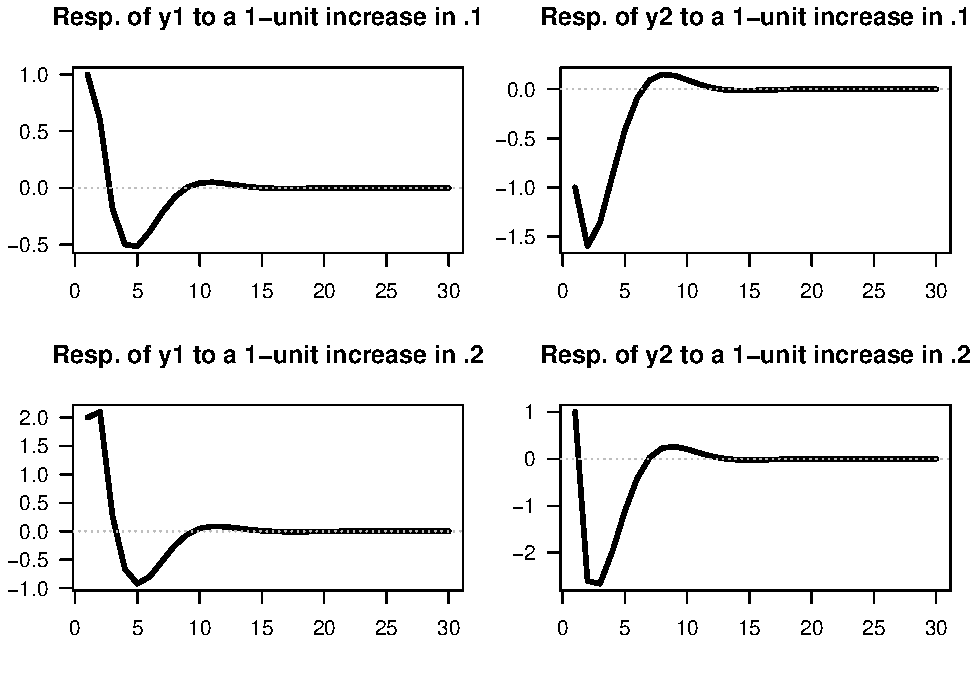
\includegraphics[width=0.95\linewidth]{IdentifStructShocks_files/figure-latex/simVAR-1} \caption{Impulse response functions (SVARMA(1,1) specified above).}\label{fig:simVAR}
\end{figure}

\end{example}

\section{Covariance-stationary VARMA models}\label{covariance-stationary-varma-models}

Let's come back to the infinite MA case (Eq. \eqref{eq:InfMA}):
\[
y_t = \mu + \sum_{h=0}^\infty \Psi_{h} \eta_{t-h}.
\]
For \(y_t\) to be covariance-stationary (and ergodic for the mean), it has to be the case that
\begin{equation}
\sum_{i=0}^\infty \|\Psi_i\| < \infty,
\label{eq:condiInfiniteMA}
\end{equation}
where \(\|A\|\) denotes a norm of the matrix \(A\) (e.g.~\(\|A\|=\sqrt{tr(AA')}\)). This notably implies that if \(y_t\) is stationary (and ergodic for the mean), then \(\|\Psi_h\|\rightarrow 0\) when \(h\) gets large.

What should be satisfied by \(\Phi_k\)'s and \(\Theta_k\)'s for a VARMA-based process (Eq. \eqref{eq:yVARMA}) to be stationary? The conditions will be similar to that we have in the univariate case. Let us introduce the following notations:
\begin{eqnarray}
y_t &=& c + \underbrace{\Phi_1 y_{t-1} + \dots +\Phi_p y_{t-p}}_{\color{blue}{\mbox{AR component}}} +  \\
&&\underbrace{B \eta_t - \Theta_1 B \eta_{t-1} - \dots - \Theta_q B \eta_{t-q}}_{\color{red}{\mbox{MA component}}} \nonumber\\
&\Leftrightarrow& \underbrace{ \color{blue}{(I - \Phi_1 L - \dots - \Phi_p L^p)}}_{= \color{blue}{\Phi(L)}}y_t = c +  \underbrace{ \color{red}{(I + \Theta_1 L + \ldots + \Theta_q L^q)}}_{=\color{red}{\Theta(L)}} B \eta_{t}. \nonumber
\label{eq:VARMA2}
\end{eqnarray}

Process \(y_t\) is stationary iff the roots of \(\det(\Phi(z))=0\) are strictly outside the unit circle or, equivalently, iff the eigenvalues of
\begin{equation}
\underbrace{\Phi}_{np \times np} = \left[\begin{array}{cccc}
\Phi_{1} & \Phi_{2} & \cdots & \Phi_{p}\\
I & 0 & \cdots & 0\\
0 & \ddots & 0 & 0\\
0 & 0 & I & 0\end{array}\right]
\label{eq:matrixPHI}
\end{equation}
lie strictly within the unit circle. Hence, as is the case for univariate processes, the covariance-stationarity of a VARMA model depends only on the specification of its AR part.

Let's derive the first two unconditional moments of a (covariance-stationary) VARMA process.

Eq. \eqref{eq:VARMA2} gives \(\mathbb{E}(\Phi(L)y_t)=c\), therefore \(\Phi(1)\mathbb{E}(y_t)=c\), or
\[
\mathbb{E}(y_t) = (I - \Phi_1 - \dots - \Phi_p)^{-1}c.
\]
The autocovariances of \(y_t\) can be deduced from the infinite MA representation (Eq. \eqref{eq:InfMA}). We have:
\[
\gamma_j \equiv \mathbb{C}ov(y_t,y_{t-j}) = \sum_{i=j}^\infty \Psi_i \Psi_{i-j}'.
\]
Indeed:
\begin{eqnarray*}
\mathbb{C}ov(y_t,y_{t-j}) &=& \mathbb{E}\left(\left[\sum_{h=0}^\infty \Psi_{h} \eta_{t-h}\right]\left[\sum_{h=0}^\infty \Psi_{h} \eta_{t-j-h}\right]'\right)\\
&=& \mathbb{E}\left(\left[\sum_{i=0}^{j-1} \Psi_{i} \eta_{t-i}+\sum_{i=j}^\infty \Psi_{i} \eta_{t-i}\right]\left[\sum_{i=j}^\infty \Psi_{i-j} \eta_{t-i}\right]'\right)\\
&=&\mathbb{E}\left(\sum_{i=j}^\infty \Psi_{i} \eta_{t-i}\eta_{t-i}'\Psi_{i-j}'\right)= \sum_{i=j}^\infty \Psi_i \Psi_{i-j}'.
\end{eqnarray*}
(Remark: This infinite sum exists as soon as Eq. \eqref{eq:condiInfiniteMA} is satisfied.)

Conditional means and autocovariances can also be deduced from Eq. \eqref{eq:InfMA}. For \(0 \le h\) and \(0 \le h_1 \le h_2\):
\begin{eqnarray*}
\mathbb{E}_t(y_{t+h}) &=& \mu + \sum_{k=0}^\infty \Psi_{k+h} \eta_{t-k} \\
\mathbb{C}ov_t(y_{t+1+h_1},y_{t+1+h_2}) &=& \sum_{k=0}^{h_1} \Psi_{k}\Psi_{k+h_2-h_1}',
\end{eqnarray*}
where \(\mathbb{E}_t\) and \(\mathbb{C}ov_t\) denote the expectation and covariance conditional on \(\{\eta_t,\eta_{t-1},\dots\}\).\footnote{For VAR models, this information set coincides with \(\{y_t,y_{t-1},\ldots\}\). For VARMA models, this equivalence holds only if the model is fundamental, meaning that the moving-average operator \(\Theta(L)\) is invertible---i.e., \(\det(\Theta(z))\neq0\) for all \(|z|\le1\), so that the innovations can be recovered from current and past \(y_t\).}

The previous formula implies in particular that the forecasting error \(y_{t+h} - \mathbb{E}_t(y_{t+h})\) has a variance equal to:
\[
\boxed{\mathbb{V}ar_t(y_{t+h}) = \sum_{k=0}^{h-1} \Psi_{k}\Psi_{k}'.}
\]
Because the components of \(\eta_t\) are mutually and serially independent (and therefore uncorrelated), we have:
\[
\mathbb{V}ar(\Psi_k \eta_{t-k}) = \mathbb{V}ar\left(\sum_{i=1}^n \psi_{k,i} \eta_{i,t-k}\right)  = \sum_{i=1}^n \psi_{k,i}\psi_{k,i}',
\]
where \(\psi_{k,i}\) denotes the \(i^{th}\) column of \(\Psi_k\). This suggests the following decomposition of the variance of the forecast error (called \textbf{variance decomposition}):
\[
\mathbb{V}ar_t(y_{t+h}) = \sum_{i=1}^n \underbrace{\sum_{k=0}^{h-1}\psi_{k,i}\psi_{k,i}'.}_{\mbox{Contribution of $\eta_{i,t}$}}
\]

To illustrate, let us use the VAR(2) model proposed above, in Example \ref{exm:IRFVAR}. As explained above, the variance decomposition directly results from the knowledge of IRFs (shown in Figure \ref{fig:simVAR2}):

\begin{example}[Variance decomposition in the context of a VAR(2) defined.]
\protect\hypertarget{exm:IRFVARvardec}{}\label{exm:IRFVARvardec}

The chunk below computes, for different horizons, the shares of the variances of the two variables that are accounted for by each of the two components of \(\eta_t\) in the context of the model proposed in Example \ref{exm:IRFVAR}.

\begin{Shaded}
\begin{Highlighting}[]
\NormalTok{Phi }\OtherTok{\textless{}{-}} \FunctionTok{array}\NormalTok{(}\ConstantTok{NaN}\NormalTok{,}\FunctionTok{c}\NormalTok{(}\DecValTok{2}\NormalTok{,}\DecValTok{2}\NormalTok{,}\DecValTok{2}\NormalTok{)) }\CommentTok{\# (2,2,2) for (n,n,p)}
\NormalTok{Phi[,,}\DecValTok{1}\NormalTok{] }\OtherTok{\textless{}{-}} \FunctionTok{matrix}\NormalTok{(}\FunctionTok{c}\NormalTok{(.}\DecValTok{6}\NormalTok{,}\DecValTok{0}\NormalTok{,.}\DecValTok{2}\NormalTok{,.}\DecValTok{5}\NormalTok{),}\DecValTok{2}\NormalTok{,}\DecValTok{2}\NormalTok{)}
\NormalTok{Phi[,,}\DecValTok{2}\NormalTok{] }\OtherTok{\textless{}{-}} \FunctionTok{matrix}\NormalTok{(}\FunctionTok{c}\NormalTok{(}\SpecialCharTok{{-}}\NormalTok{.}\DecValTok{1}\NormalTok{,.}\DecValTok{2}\NormalTok{,.}\DecValTok{1}\NormalTok{,.}\DecValTok{3}\NormalTok{),}\DecValTok{2}\NormalTok{,}\DecValTok{2}\NormalTok{)}
\NormalTok{B }\OtherTok{\textless{}{-}} \FunctionTok{matrix}\NormalTok{(}\FunctionTok{c}\NormalTok{(.}\DecValTok{5}\NormalTok{,}\SpecialCharTok{{-}}\DecValTok{1}\NormalTok{,}\FloatTok{1.5}\NormalTok{,.}\DecValTok{8}\NormalTok{),}\DecValTok{2}\NormalTok{,}\DecValTok{2}\NormalTok{)}
\FunctionTok{make\_variance\_decompo}\NormalTok{(Phi,B,}\AttributeTok{maxHorizon=}\DecValTok{30}\NormalTok{)}
\end{Highlighting}
\end{Shaded}

\begin{figure}
\centering
\pandocbounded{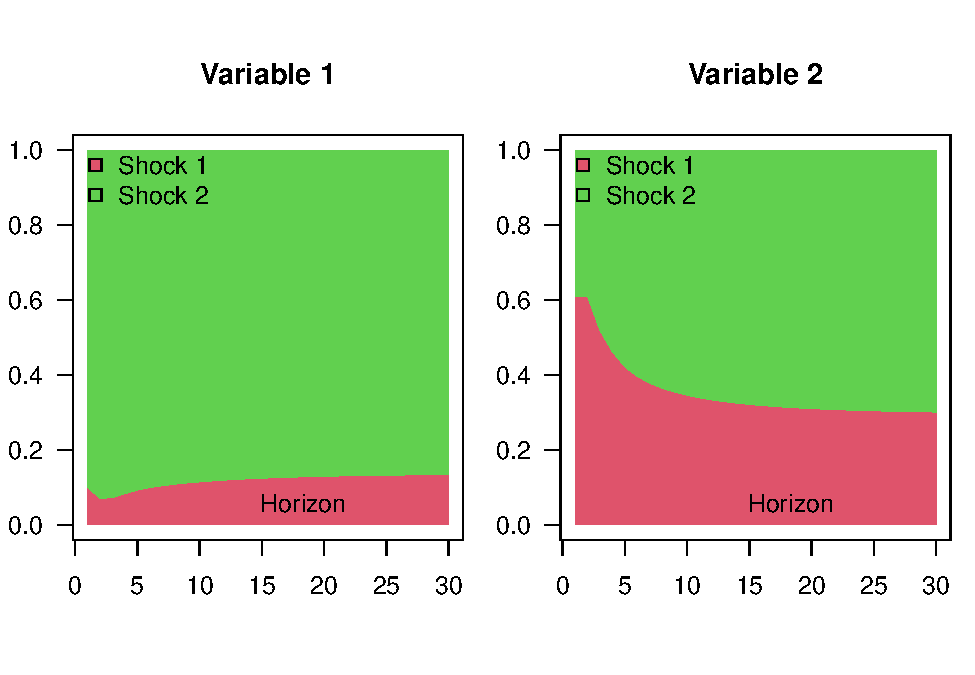
\includegraphics[keepaspectratio]{IdentifStructShocks_files/figure-latex/simVAR2vardec-1.pdf}}
\caption{\label{fig:simVAR2vardec}Variance decomposition of a VAR(2) model.}
\end{figure}

\end{example}

\section{VAR estimation}\label{estimVAR}

This section discusses the estimation of VAR models.\footnote{The estimation of VARMA models is introduced in Appendix \ref{AppEstimVARMA}.} Eq. \eqref{eq:yVAR} can be written:
\[
y_{t}=c+\Phi(L)y_{t-1}+\varepsilon_{t},
\]
with \(\Phi(L) = \Phi_1 + \Phi_2 L + \dots + \Phi_p L^{p-1}\), and where the reduced-form shocks (\(\varepsilon_{t}\)) are white noise shocks.\footnote{That is, these shocks are such that \(\mathbb{E}(\varepsilon_{t})=0\), and \(\mathbb{C}ov(\varepsilon_{t},\varepsilon_{t-k})=\Omega\) if \(k=0\), and a zero matrix if \(k \ne 0\).}

Using \citet{Hamilton_1994}'s notations, denote with \(\Pi\) the matrix \(\left[\begin{array}{ccccc}
c & \Phi_{1} & \Phi_{2} & \ldots & \Phi_{p}\end{array}\right]'\) and with \(x_{t}\) the vector \(\left[\begin{array}{ccccc}
1 & y'_{t-1} & y'_{t-2} & \ldots & y'_{t-p}\end{array}\right]'\), we have:
\begin{equation}
y_{t}= \Pi'x_{t} + \varepsilon_{t}.
\label{eq:PIVAR}
\end{equation}

The previous representation is convenient to discuss the estimation of the VAR model, as parameters are gathered in two matrices only: \(\Pi\) and \(\Omega\) (where \(\Omega = \mathbb{V}ar (\varepsilon_t)\)).

\subsection{Maximum Likelihood Estimation (MLE) when the shocks are Gaussian}\label{maximum-likelihood-estimation-mle-when-the-shocks-are-gaussian}

Let us start with the case where the shocks are i.i.d. Gaussian. We then have:
\[
y_{t}\mid y_{t-1},y_{t-2},\ldots\sim \mathcal{N}(c+\Phi_{1}y_{t-1}+\ldots\Phi_{p}y_{t-p},\Omega).
\]

\begin{proposition}[MLE of a Gaussian VAR]
\protect\hypertarget{prp:estimVARGaussian}{}\label{prp:estimVARGaussian}If \(y_t\) follows a VAR(\(p\)) (see Definition \ref{def:SVAR}), and if \(\varepsilon_t \sim \,i.i.d.\,\mathcal{N}(0,\Omega)\), then the ML estimate of \(\Pi\), denoted by \(\hat{\Pi}\) (see Eq. \eqref{eq:PIVAR}), is given by
\begin{equation}
\hat{\Pi}=\left[\sum_{t=1}^{T}x_{t}x'_{t}\right]^{-1}\left[\sum_{t=1}^{T}y_{t}'x_{t}\right]= (\mathbf{X}'\mathbf{X})^{-1}\mathbf{X}'\mathbf{y},
\label{eq:Pi}
\end{equation}
where \(\mathbf{X}\) is the \(T \times (1+np)\) matrix whose \(t^{th}\) row is \(x_t\) and where \(\mathbf{y}\) is the \(T \times n\) matrix whose \(t^{th}\) row is \(y_{t}'\).

That is, the \(i^{th}\) column of \(\hat{\Pi}\) (\(b_i\), say) is the OLS estimate of \(\beta_i\), where:
\begin{equation}
y_{i,t} = \beta_i'x_t + \varepsilon_{i,t},
\label{eq:betayx}
\end{equation}
(i.e., \(\beta_i' = [c_i,\phi_{i,1}',\dots,\phi_{i,p}']'\)).

The ML estimate of \(\Omega\), denoted by \(\hat{\Omega}\), coincides with the sample covariance matrix of the \(n\) series of the OLS residuals in Eq. \eqref{eq:betayx}, i.e.:
\begin{equation}
\hat{\Omega} = \frac{1}{T} \sum_{i=1}^T \hat{\varepsilon}_t\hat{\varepsilon}_t',\quad\mbox{with } \hat{\varepsilon}_t= y_t - \hat{\Pi}'x_t.
\end{equation}

The asymptotic distributions of these estimators are the ones resulting from standard OLS formula.
\end{proposition}

\begin{proof}
See Appendix \ref{AppendixProof}.
\end{proof}

The simplicity of the VAR framework and the tractability of its MLE open the way to convenient econometric testing. Let's illustrate this with the likelihood ratio test (see Def. \ref{def:LR}). The maximum value achieved by the MLE is
\[
\log\mathcal{L}(Y_{T};\hat{\Pi},\hat{\Omega}) = -\frac{Tn}{2}\log(2\pi)+\frac{T}{2}\log\left|\hat{\Omega}^{-1}\right| -\frac{1}{2}\sum_{t=1}^{T}\left[\hat{\varepsilon}_{t}'\hat{\Omega}^{-1}\hat{\varepsilon}_{t}\right].
\]
The last term is:
\begin{eqnarray*}
\sum_{t=1}^{T}\hat{\varepsilon}_{t}'\hat{\Omega}^{-1}\hat{\varepsilon}_{t} &=& \mbox{Tr}\left[\sum_{t=1}^{T}\hat{\varepsilon}_{t}'\hat{\Omega}^{-1}\hat{\varepsilon}_{t}\right] = \mbox{Tr}\left[\sum_{t=1}^{T}\hat{\Omega}^{-1}\hat{\varepsilon}_{t}\hat{\varepsilon}_{t}'\right]\\
&=&\mbox{Tr}\left[\hat{\Omega}^{-1}\sum_{t=1}^{T}\hat{\varepsilon}_{t}\hat{\varepsilon}_{t}'\right] = \mbox{Tr}\left[\hat{\Omega}^{-1}\left(T\hat{\Omega}\right)\right]=Tn.
\end{eqnarray*}
Therefore, the optimized log-likelihood is simply obtained by:
\begin{equation}
\log\mathcal{L}(Y_{T};\hat{\Pi},\hat{\Omega})=-(Tn/2)\log(2\pi)+(T/2)\log\left|\hat{\Omega}^{-1}\right|-Tn/2.
\label{eq:optimzedLogL}
\end{equation}

Having the optimized likelihood in analytical form allows for flexible applications of the likelihood ratio (LR) test (Def. \ref{def:LR}).

\begin{example}[Ad-hoc lag selection based on the LR test]
\protect\hypertarget{exm:AdhocLagSelectLR}{}\label{exm:AdhocLagSelectLR}Suppose we want to test whether a system of variables follows a VAR(\(p_0\)) process (the null hypothesis) against an alternative specification with \(p_1\) lags, where \(p_1 > p_0\).
Let \(\hat{L}_0\) and \(\hat{L}_1\) denote the maximum log-likelihoods obtained under the two specifications, respectively.
Under the null hypothesis (\(H_0\): \(p = p_0\)), the LR statistic is given by

\begin{equation}
\xi^{LR} := 2(\hat{L}_1 - \hat{L}_0)
= T \left( \log\left|\hat{\Omega}_1^{-1}\right| - \log\left|\hat{\Omega}_0^{-1}\right| \right)
\sim \chi^2\left(n^2(p_1 - p_0)\right).
\end{equation}

This statistic can be used to determine whether adding lags significantly improves the model fit.
However, including too many lags quickly exhausts degrees of freedom: with \(p\) lags, each of the \(n\) equations in the VAR includes \(n \times p\) coefficients plus an intercept term.
While adding lags always improves the in-sample fit, it can lead to over-parameterization and deteriorate the model's out-of-sample predictive performance.
\end{example}

The approach above provides an ad-hoc way to select lag length using LR tests (Def. \ref{def:LR}).
More systematic procedures rely on information criteria, which balance goodness of fit and model parsimony.
In the Gaussian case (see Eq. \eqref{eq:optimzedLogL}), common criteria include:
\begin{eqnarray*}
AIC & = & cst + \log\left|\hat{\Omega}\right| + \frac{2}{T}N \\
BIC & = & cst + \log\left|\hat{\Omega}\right| + \frac{\log T}{T}N,
\end{eqnarray*}
where \(N = p \times n^2\). In these expressions, \(\log|\hat{\Omega}|\) captures the model's goodness of fit (with smaller values indicating better fit), while the last term is a penalty that increases with the number of estimated parameters.

\begin{example}[Three-variable VAR model]
\protect\hypertarget{exm:US3varselect}{}\label{exm:US3varselect}

The following example illustrates how to estimate and analyze a three-variable VAR model using U.S. quarterly data on inflation, the output gap, and the short-term nominal interest rate.

We begin by using the \texttt{VARselect} function from the \texttt{vars} package to determine the optimal lag length for the VAR specification.

\begin{Shaded}
\begin{Highlighting}[]
\FunctionTok{library}\NormalTok{(vars)   }\CommentTok{\# provides \textquotesingle{}VARselect\textquotesingle{} function}
\FunctionTok{library}\NormalTok{(IdSS)   }\CommentTok{\# dataset is included here}

\NormalTok{First.date }\OtherTok{\textless{}{-}} \StringTok{"1959{-}04{-}01"}
\NormalTok{Last.date  }\OtherTok{\textless{}{-}} \StringTok{"2015{-}01{-}01"}

\NormalTok{data }\OtherTok{\textless{}{-}}\NormalTok{ US3var}
\NormalTok{data }\OtherTok{\textless{}{-}}\NormalTok{ data[(data}\SpecialCharTok{$}\NormalTok{Date }\SpecialCharTok{\textgreater{}=}\NormalTok{ First.date) }\SpecialCharTok{\&}\NormalTok{ (data}\SpecialCharTok{$}\NormalTok{Date }\SpecialCharTok{\textless{}=}\NormalTok{ Last.date), ]}
\NormalTok{Y }\OtherTok{\textless{}{-}} \FunctionTok{as.matrix}\NormalTok{(data[}\FunctionTok{c}\NormalTok{(}\StringTok{"infl"}\NormalTok{, }\StringTok{"y.gdp.gap"}\NormalTok{, }\StringTok{"r"}\NormalTok{)])}

\FunctionTok{VARselect}\NormalTok{(Y, }\AttributeTok{lag.max =} \DecValTok{12}\NormalTok{)}
\end{Highlighting}
\end{Shaded}

\begin{verbatim}
## $selection
## AIC(n)  HQ(n)  SC(n) FPE(n) 
##     11      3      2     11 
## 
## $criteria
##                  1            2           3          4          5          6
## AIC(n) -0.14340897 -0.323002241 -0.39796730 -0.3888482 -0.4110019 -0.5229686
## HQ(n)  -0.06661725 -0.188616726 -0.20598799 -0.1392751 -0.1038350 -0.1582079
## SC(n)   0.04658647  0.009489796  0.07702133  0.2286370  0.3489799  0.3795098
## FPE(n)  0.86641130  0.724024392  0.67182519  0.6781505  0.6635579  0.5936165
##                  7           8           9         10         11         12
## AIC(n) -0.48840029 -0.50157851 -0.44613801 -0.4950938 -0.5372138 -0.4980589
## HQ(n)  -0.06604582 -0.02163024  0.09140405  0.1000420  0.1155158  0.2122645
## SC(n)   0.55657468  0.68589305  0.88383014  0.9773709  1.0777475  1.2593990
## FPE(n)  0.61498914  0.60758020  0.64308309  0.6133871  0.5892917  0.6143270
\end{verbatim}

Next, we estimate the VAR model including an exogenous variable --- the commodity price index.

\begin{Shaded}
\begin{Highlighting}[]
\NormalTok{p }\OtherTok{\textless{}{-}} \DecValTok{6}
\NormalTok{exogen }\OtherTok{\textless{}{-}} \FunctionTok{matrix}\NormalTok{(data}\SpecialCharTok{$}\NormalTok{commo, }\AttributeTok{ncol =} \DecValTok{1}\NormalTok{); }\FunctionTok{colnames}\NormalTok{(exogen) }\OtherTok{\textless{}{-}} \StringTok{"commo"}
\NormalTok{estVAR }\OtherTok{\textless{}{-}} \FunctionTok{VAR}\NormalTok{(Y, }\AttributeTok{p =}\NormalTok{ p, }\AttributeTok{exogen =}\NormalTok{ exogen) }\CommentTok{\# estimate the VAR model}
\NormalTok{Phi }\OtherTok{\textless{}{-}} \FunctionTok{Acoef}\NormalTok{(estVAR)}
\NormalTok{eps }\OtherTok{\textless{}{-}} \FunctionTok{residuals}\NormalTok{(estVAR)}
\NormalTok{Omega }\OtherTok{\textless{}{-}} \FunctionTok{var}\NormalTok{(eps) }\CommentTok{\# covariance matrix of OLS residuals}
\NormalTok{B }\OtherTok{\textless{}{-}} \FunctionTok{t}\NormalTok{(}\FunctionTok{chol}\NormalTok{(Omega)) }\CommentTok{\# Cholesky decomposition of Omega (lower triangular)}
\end{Highlighting}
\end{Shaded}

We can now verify whether the estimated VAR is stationary:

\begin{Shaded}
\begin{Highlighting}[]
\NormalTok{PHI }\OtherTok{\textless{}{-}} \FunctionTok{make.PHI}\NormalTok{(Phi) }\CommentTok{\# autoregressive matrix in companion form}
\FunctionTok{print}\NormalTok{(}\FunctionTok{abs}\NormalTok{(}\FunctionTok{eigen}\NormalTok{(PHI)}\SpecialCharTok{$}\NormalTok{values)) }\CommentTok{\# eigenvalues must be \textless{} 1 for stationarity}
\end{Highlighting}
\end{Shaded}

\begin{verbatim}
##  [1] 0.9485855 0.9485855 0.9180083 0.8539724 0.8539724 0.7683116 0.7683116
##  [8] 0.7509592 0.7509592 0.7465920 0.7465920 0.7392400 0.7392400 0.6720905
## [15] 0.6720905 0.4474043 0.4474043 0.3904400
\end{verbatim}

All eigenvalues have moduli smaller than one, confirming that the system is stationary.

We then compute and display the impulse response functions (IRFs) using the Cholesky identification approach (see Section \ref{Cholesky}), where the impact matrix \(B\) comes from the Cholesky factorization of \(\Omega = \mathbb{V}ar(\varepsilon_t)\).

\begin{Shaded}
\begin{Highlighting}[]
\NormalTok{n }\OtherTok{\textless{}{-}} \FunctionTok{dim}\NormalTok{(Y)[}\DecValTok{2}\NormalTok{] }\CommentTok{\# number of endogenous variables}
\FunctionTok{par}\NormalTok{(}\AttributeTok{mfrow =} \FunctionTok{c}\NormalTok{(n, n))}
\FunctionTok{par}\NormalTok{(}\AttributeTok{plt =} \FunctionTok{c}\NormalTok{(.}\DecValTok{3}\NormalTok{, .}\DecValTok{95}\NormalTok{, .}\DecValTok{2}\NormalTok{, .}\DecValTok{8}\NormalTok{))}
\NormalTok{Model }\OtherTok{\textless{}{-}} \FunctionTok{list}\NormalTok{(}\AttributeTok{c =}\NormalTok{ c, }\AttributeTok{Phi =}\NormalTok{ Phi, }\AttributeTok{B =}\NormalTok{ B)}
\NormalTok{names.var }\OtherTok{\textless{}{-}} \FunctionTok{c}\NormalTok{(}\StringTok{"Inflation"}\NormalTok{, }\StringTok{"Output gap"}\NormalTok{, }\StringTok{"Interest rate"}\NormalTok{)}

\ControlFlowTok{for}\NormalTok{ (variable }\ControlFlowTok{in} \DecValTok{1}\SpecialCharTok{:}\NormalTok{n) \{}
  \ControlFlowTok{for}\NormalTok{ (shock }\ControlFlowTok{in} \DecValTok{1}\SpecialCharTok{:}\NormalTok{n) \{}
\NormalTok{    eta0 }\OtherTok{\textless{}{-}} \FunctionTok{rep}\NormalTok{(}\DecValTok{0}\NormalTok{, n)}
\NormalTok{    eta0[shock] }\OtherTok{\textless{}{-}} \DecValTok{1}
\NormalTok{    res.sim }\OtherTok{\textless{}{-}} \FunctionTok{simul.VAR}\NormalTok{(}\AttributeTok{c =} \ConstantTok{NaN}\NormalTok{, Phi, B, }\AttributeTok{nb.sim =} \DecValTok{30}\NormalTok{, }\AttributeTok{indic.IRF =} \DecValTok{1}\NormalTok{,}
                         \AttributeTok{u.shock =}\NormalTok{ eta0)}
    \FunctionTok{plot}\NormalTok{(res.sim[, variable], }\AttributeTok{type =} \StringTok{"l"}\NormalTok{, }\AttributeTok{lwd =} \DecValTok{2}\NormalTok{, }\AttributeTok{las =} \DecValTok{1}\NormalTok{,}
         \AttributeTok{xlab =} \StringTok{""}\NormalTok{, }\AttributeTok{ylab =} \FunctionTok{ifelse}\NormalTok{(shock}\SpecialCharTok{==}\DecValTok{1}\NormalTok{,}
                                  \FunctionTok{paste}\NormalTok{(}\StringTok{"Resp. of "}\NormalTok{,}
\NormalTok{                                              names.var[variable],}\StringTok{"..."}\NormalTok{,}\AttributeTok{sep=}\StringTok{""}\NormalTok{),}\StringTok{""}\NormalTok{),}
         \AttributeTok{main =} \FunctionTok{ifelse}\NormalTok{(variable}\SpecialCharTok{==}\DecValTok{1}\NormalTok{,}\FunctionTok{paste}\NormalTok{(}\StringTok{"... to shock η"}\NormalTok{, shock, }\AttributeTok{sep =} \StringTok{""}\NormalTok{),}\StringTok{""}\NormalTok{)}
\NormalTok{         )\}}
\NormalTok{\}}
\end{Highlighting}
\end{Shaded}

\begin{figure}
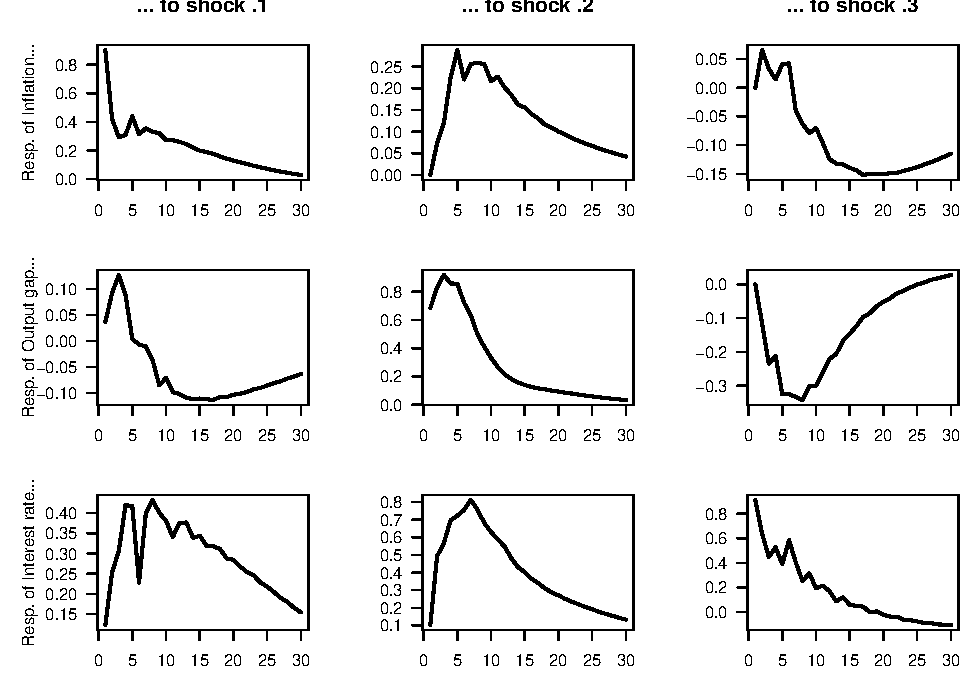
\includegraphics[width=0.95\linewidth]{IdentifStructShocks_files/figure-latex/US3varIRFs1-1} \caption{Impulse response functions for a 3-variable VAR model estimated on U.S. quarterly data.}\label{fig:US3varIRFs1}
\end{figure}

Finally, we compute the variance decomposition associated with the same model.

\begin{Shaded}
\begin{Highlighting}[]
\FunctionTok{make\_variance\_decompo}\NormalTok{(Phi, B, }\AttributeTok{maxHorizon =} \DecValTok{50}\NormalTok{,}
                      \AttributeTok{names.var =} \FunctionTok{c}\NormalTok{(}\StringTok{"Inflation"}\NormalTok{, }\StringTok{"Real activity"}\NormalTok{,}
                                    \StringTok{"Short{-}term rate"}\NormalTok{))}
\end{Highlighting}
\end{Shaded}

\begin{figure}
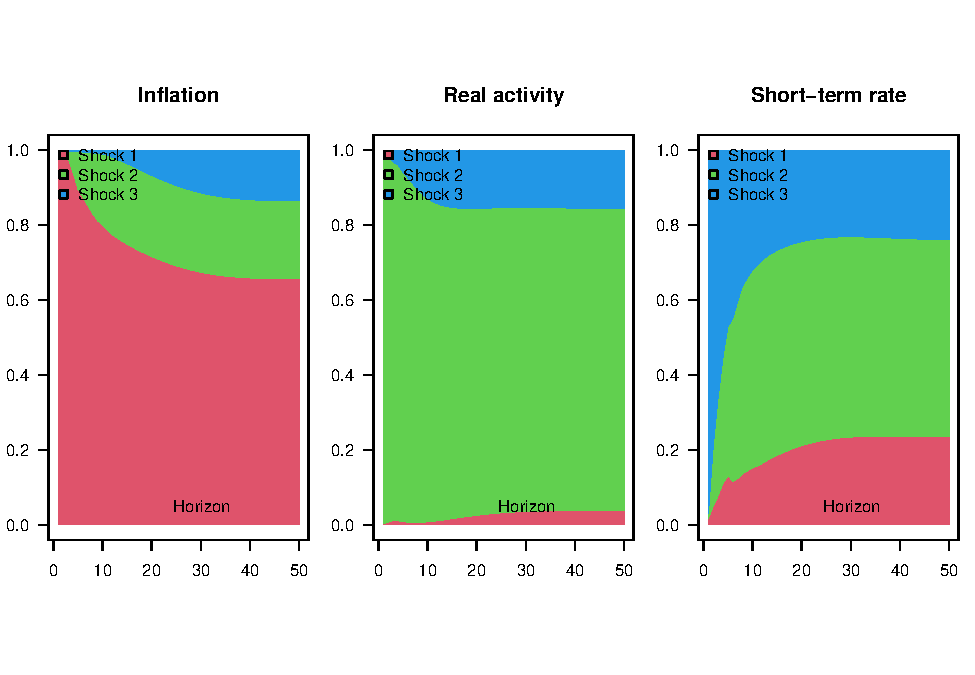
\includegraphics[width=0.95\linewidth]{IdentifStructShocks_files/figure-latex/US3varVARdecomp-1} \caption{Variance decomposition for a 3-variable VAR model estimated on U.S. quarterly data.}\label{fig:US3varVARdecomp}
\end{figure}

\end{example}

\subsection{Asymptotic distribution of the OLS estimates}\label{asymptotic-distribution-of-the-ols-estimates}

As stated by the following proposition, when the shocks \(\varepsilon_t\) are not Gaussian, then the OLS regressions still provide consistent estimates of the model parameters.

\begin{proposition}[Asymptotic distribution of the OLS estimate of VAR coefficients (for one variable)]
\protect\hypertarget{prp:OLSVAR}{}\label{prp:OLSVAR}If \(y_t\) follows a VAR model, as defined in Definition \ref{def:SVAR}, we have:
\[
\sqrt{T}(\mathbf{b}_i-\beta_i) =  \underbrace{\left[\frac{1}{T}\sum_{t=p}^T x_t x_t' \right]^{-1}}_{\overset{p}{\rightarrow} \mathbf{Q}^{-1}}
\underbrace{\sqrt{T} \left[\frac{1}{T}\sum_{t=1}^T x_t\varepsilon_{i,t} \right]}_{\overset{d}{\rightarrow} \mathcal{N}(0,\sigma_i^2\mathbf{Q})},
\]
where \(\sigma_i = \mathbb{V}ar(\varepsilon_{i,t})\) and where \(\mathbf{Q} = \mbox{plim }\frac{1}{T}\sum_{t=p}^T x_t x_t'\) is given by:
\begin{equation}
\mathbf{Q} = \left[
\begin{array}{ccccc}
1 & \mu' &\mu' & \dots & \mu' \\
\mu & \gamma_0 + \mu\mu' & \gamma_1 + \mu\mu' & \dots & \gamma_{p-1} + \mu\mu'\\
\mu & \gamma_1 + \mu\mu' & \gamma_0 + \mu\mu' & \dots & \gamma_{p-2} + \mu\mu'\\
\vdots &\vdots &\vdots &\dots &\vdots \\
\mu & \gamma_{p-1} + \mu\mu' & \gamma_{p-2} + \mu\mu' & \dots & \gamma_{0} + \mu\mu'
\end{array}
\right],
\label{eq:Qols}
\end{equation}
where \(\gamma_j\) is the unconditional autocovariance matrix of order \(j\) of \(y_t\), i.e., \(\gamma_i = \mathbb{C}ov(y_{t},y_{t-j})\).
\end{proposition}

\begin{proof}
See Appendix \ref{AppendixProof}.
\end{proof}

However, since \(x_t\) correlates to \(\varepsilon_s\) for \(s<t\), the OLS estimator \(\mathbf{b}_i\) of \(\boldsymbol\beta_i\) is biased in small sample. (That is also the case for the ML estimator.) Indeed, denoting by \(\boldsymbol\varepsilon_i\) the \(T \times 1\) vector of \(\varepsilon_{i,t}\)'s, and using the notations of \(b_i\) and \(\beta_i\) introduced in Proposition \ref{prp:estimVARGaussian}, we have:
\begin{equation}
\mathbf{b}_i = \beta_i + (\mathbf{X}'\mathbf{X})^{-1}\mathbf{X}'\boldsymbol\varepsilon_i.
\label{eq:olsar1}
\end{equation}

We have non-zero correlation between \(x_t\) and \(\varepsilon_{i,s}\) for \(s<t\) and, therefore, \(\mathbb{E}[(\mathbf{X}'\mathbf{X})^{-1}\mathbf{X}'\boldsymbol\varepsilon_i] \ne 0\).

However, as stated by Proposition \ref{prp:OLSVAR} when \(y_t\) is covariance stationary, then \(\frac{1}{n}\mathbf{X}'\mathbf{X}\) converges to a positive definite matrix \(\mathbf{Q}\), and \(\frac{1}{n}X'\boldsymbol\varepsilon_i\) converges to 0. Hence \(\mathbf{b}_i \overset{p}{\rightarrow} \beta_i\).

The next proposition extends Proposition \ref{prp:OLSVAR} by incorporating the covariances between different \(\beta_i\)'s and by characterizing the asymptotic distribution of the ML estimator of \(\Omega\). In other words, it delivers the full asymptotic distribution of the model parameters. This result is particularly useful for Monte Carlo procedures that require drawing from this asymptotic distribution (see Section \ref{MonteCarlo}).

\begin{proposition}[Asymptotic distribution of the OLS estimates]
\protect\hypertarget{prp:OLSVAR2}{}\label{prp:OLSVAR2}If \(y_t\) follows a VAR model, as defined in Definition \ref{def:SVAR}, we have:
\begin{equation}
\sqrt{T}\left[
\begin{array}{c}
vec(\hat\Pi - \Pi)\\
vec(\hat\Omega - \Omega)
\end{array}
\right]
\sim \mathcal{N}\left(0,
\left[
\begin{array}{cc}
\Omega \otimes \mathbf{Q}^{-1} & 0\\
0 & \Sigma_{22}
\end{array}
\right]\right),
\label{eq:asymptPi}
\end{equation}
where the component of \(\Sigma_{22}\) corresponding to the covariance between \(\hat\sigma_{i,j}\) and \(\hat\sigma_{k,l}\) (for \(i,j,l,m \in \{1,\dots,n\}^4\)) is equal to \(\sigma_{i,l}\sigma_{j,m}+\sigma_{i,m}\sigma_{j,l}\).
\end{proposition}

\begin{proof}
See, e.g., \citet{Hamilton_1994}, Appendix of Chapter 11.
\end{proof}

In practice, to use the previous proposition (for instance to implement Monte-Carlo simulations), \(\Omega\) is replaced with \(\hat{\Omega}\), \(\mathbf{Q}\) is replaced with \(\hat{\mathbf{Q}} = \frac{1}{T}\sum_{t=p}^T x_t x_t'\) and \(\Sigma\) with the matrix whose components are of the form \(\hat\sigma_{i,l}\hat\sigma_{j,m}+\hat\sigma_{i,m}\hat\sigma_{j,l}\), where the \(\hat\sigma_{i,l}\)'s are the components of \(\hat\Omega\).

\subsection{Specification tests}\label{specification-tests}

After estimating a VAR, it is important to check that the model assumptions hold. In particular, we verify:

\begin{enumerate}
\def\labelenumi{\arabic{enumi}.}
\item
  \textbf{Stationarity of the data} (often checked before estimation). If the variables are non-stationary and not cointegrated, the asymptotic distributions of the estimates are not valid and standard inference (including likelihood-based tests) breaks down. In practice, one typically inspects unit-root tests or relies on economic knowledge about integration and cointegration properties. \(\Rightarrow\) Remedy: transform the data to make them stationary (removing deterministic trends, or using differences), or use Vector Error-Correction Models (VECM).
\item
  \textbf{Absence of residual autocorrelation}. If residuals are serially correlated, the dynamic specification of the VAR is inadequate (e.g., too few lags). This leads to biased estimates of the constant and the \(\Phi_i\) matrices and, consequently, biased impulse response functions. \(\Rightarrow\) Remedy: increase the lag length or reconsider the model specification (e.g., adding variables, or transforming the variables).
\item
  \textbf{Homoskedasticity}. If residuals exhibit heteroskedasticity, OLS estimates remain consistent under mild conditions, but they are no longer efficient, and standard errors become unreliable in finite samples in particular. If they are based on the asymptotic distribution, confidence intervals for coefficients and impulse responses may be misleading. \(\Rightarrow\) Remedy: use heteroskedasticity-robust inference (e.g., bootstrapped inference methods, see Chapter \ref{Inference}), or adopt models allowing for time-varying volatility (e.g., VAR-GARCH, stochastic-volatility VAR).
\item
  \textbf{Normality of residuals}. Non-normality does not affect consistency of OLS estimates, but it weakens the validity of inference and ML-based tests, especially in small samples. Confidence bands for impulse responses may be distorted under heavy tails or skewness. \(\Rightarrow\) Remedy: use bootstrap inference for hypothesis testing and IRFs.
\end{enumerate}

\begin{example}[Bivariate model for Switzerland]
\protect\hypertarget{exm:BivariateVARCHE}{}\label{exm:BivariateVARCHE}

In this example, we consider a bivariate model capturing the joint dynamics of Swiss inflation and GDP growth rates.

\begin{Shaded}
\begin{Highlighting}[]
\NormalTok{First.date }\OtherTok{\textless{}{-}} \StringTok{"1980{-}01{-}01"}
\NormalTok{Last.date  }\OtherTok{\textless{}{-}} \StringTok{"2025{-}01{-}01"}
\NormalTok{data }\OtherTok{\textless{}{-}}\NormalTok{ international[,}\FunctionTok{c}\NormalTok{(}\StringTok{"date"}\NormalTok{,}\StringTok{"CPI\_CHE"}\NormalTok{,}\StringTok{"GDP\_CHE"}\NormalTok{)]}
\NormalTok{data }\OtherTok{\textless{}{-}}\NormalTok{ data[(data}\SpecialCharTok{$}\NormalTok{date }\SpecialCharTok{\textgreater{}=}\NormalTok{ First.date) }\SpecialCharTok{\&}\NormalTok{ (data}\SpecialCharTok{$}\NormalTok{date }\SpecialCharTok{\textless{}=}\NormalTok{ Last.date), ]}
\NormalTok{data }\OtherTok{\textless{}{-}}\NormalTok{ data[}\FunctionTok{complete.cases}\NormalTok{(data),]}
\NormalTok{Y }\OtherTok{\textless{}{-}}\NormalTok{ data[,}\FunctionTok{c}\NormalTok{(}\StringTok{"CPI\_CHE"}\NormalTok{,}\StringTok{"GDP\_CHE"}\NormalTok{)]}
\FunctionTok{par}\NormalTok{(}\AttributeTok{mfrow=}\FunctionTok{c}\NormalTok{(}\DecValTok{1}\NormalTok{,}\DecValTok{1}\NormalTok{));}\FunctionTok{par}\NormalTok{(}\AttributeTok{plt=}\FunctionTok{c}\NormalTok{(.}\DecValTok{1}\NormalTok{,.}\DecValTok{95}\NormalTok{,.}\DecValTok{15}\NormalTok{,.}\DecValTok{95}\NormalTok{))}
\FunctionTok{plot}\NormalTok{(data}\SpecialCharTok{$}\NormalTok{date,data}\SpecialCharTok{$}\NormalTok{CPI\_CHE,}\AttributeTok{type=}\StringTok{"l"}\NormalTok{,}\AttributeTok{lwd=}\DecValTok{2}\NormalTok{,}\AttributeTok{las=}\DecValTok{1}\NormalTok{,}\AttributeTok{ylim=}\FunctionTok{c}\NormalTok{(}\SpecialCharTok{{-}}\DecValTok{7}\NormalTok{,}\DecValTok{11}\NormalTok{),}
     \AttributeTok{xlab=}\StringTok{""}\NormalTok{,}\AttributeTok{ylab=}\StringTok{""}\NormalTok{)}
\FunctionTok{grid}\NormalTok{()}
\FunctionTok{lines}\NormalTok{(data}\SpecialCharTok{$}\NormalTok{date,data}\SpecialCharTok{$}\NormalTok{GDP\_CHE,}\AttributeTok{lwd=}\DecValTok{2}\NormalTok{,}\AttributeTok{col=}\StringTok{"grey"}\NormalTok{)}
\end{Highlighting}
\end{Shaded}

\begin{figure}
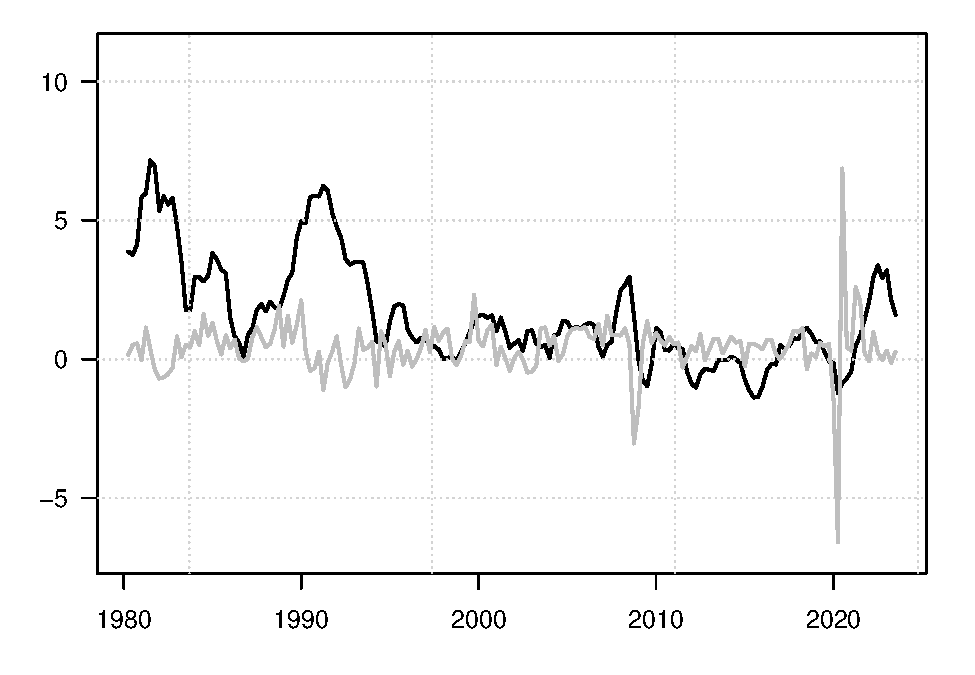
\includegraphics[width=0.95\linewidth]{IdentifStructShocks_files/figure-latex/US2varCHE-1} \caption{Inflation and GDP growth rates. Percent change from year ago.}\label{fig:US2varCHE}
\end{figure}

\begin{Shaded}
\begin{Highlighting}[]
\FunctionTok{library}\NormalTok{(tseries)}
\end{Highlighting}
\end{Shaded}

\begin{verbatim}
## Registered S3 method overwritten by 'quantmod':
##   method            from
##   as.zoo.data.frame zoo
\end{verbatim}

\begin{Shaded}
\begin{Highlighting}[]
\NormalTok{test.adf.Y1  }\OtherTok{\textless{}{-}} \FunctionTok{adf.test}\NormalTok{(Y[,}\DecValTok{1}\NormalTok{],}\AttributeTok{k=}\DecValTok{16}\NormalTok{)}\SpecialCharTok{$}\NormalTok{p.value}
\NormalTok{test.adf.Y2  }\OtherTok{\textless{}{-}} \FunctionTok{adf.test}\NormalTok{(Y[,}\DecValTok{2}\NormalTok{],}\AttributeTok{k=}\DecValTok{16}\NormalTok{)}\SpecialCharTok{$}\NormalTok{p.value}
\NormalTok{test.pp.Y1   }\OtherTok{\textless{}{-}} \FunctionTok{pp.test}\NormalTok{(Y[,}\DecValTok{1}\NormalTok{])}\SpecialCharTok{$}\NormalTok{p.value}
\NormalTok{test.pp.Y2   }\OtherTok{\textless{}{-}} \FunctionTok{pp.test}\NormalTok{(Y[,}\DecValTok{2}\NormalTok{])}\SpecialCharTok{$}\NormalTok{p.value}
\end{Highlighting}
\end{Shaded}

\begin{verbatim}
## Warning in pp.test(Y[, 2]): p-value smaller than printed p-value
\end{verbatim}

\begin{Shaded}
\begin{Highlighting}[]
\NormalTok{test.kpss.Y1 }\OtherTok{\textless{}{-}} \FunctionTok{kpss.test}\NormalTok{(Y[,}\DecValTok{1}\NormalTok{])}\SpecialCharTok{$}\NormalTok{p.value}
\end{Highlighting}
\end{Shaded}

\begin{verbatim}
## Warning in kpss.test(Y[, 1]): p-value smaller than printed p-value
\end{verbatim}

\begin{Shaded}
\begin{Highlighting}[]
\NormalTok{test.kpss.Y2 }\OtherTok{\textless{}{-}} \FunctionTok{kpss.test}\NormalTok{(Y[,}\DecValTok{2}\NormalTok{])}\SpecialCharTok{$}\NormalTok{p.value}
\end{Highlighting}
\end{Shaded}

\begin{verbatim}
## Warning in kpss.test(Y[, 2]): p-value greater than printed p-value
\end{verbatim}

\begin{Shaded}
\begin{Highlighting}[]
\NormalTok{test.adf  }\OtherTok{\textless{}{-}} \FunctionTok{c}\NormalTok{(test.adf.Y1,test.adf.Y2)}
\NormalTok{test.pp   }\OtherTok{\textless{}{-}} \FunctionTok{c}\NormalTok{(test.pp.Y1,test.pp.Y2)}
\NormalTok{test.kpss }\OtherTok{\textless{}{-}} \FunctionTok{c}\NormalTok{(test.kpss.Y1,test.kpss.Y2)}
\FunctionTok{rbind}\NormalTok{(test.adf,test.pp,test.kpss)}
\end{Highlighting}
\end{Shaded}

\begin{verbatim}
##                 [,1]       [,2]
## test.adf  0.26339041 0.03910545
## test.pp   0.06972378 0.01000000
## test.kpss 0.01000000 0.10000000
\end{verbatim}

Estimate the model parameters for a given lag choice:

\begin{Shaded}
\begin{Highlighting}[]
\NormalTok{p }\OtherTok{\textless{}{-}} \DecValTok{2}
\NormalTok{estVAR }\OtherTok{\textless{}{-}} \FunctionTok{VAR}\NormalTok{(Y, }\AttributeTok{p =}\NormalTok{ p) }\CommentTok{\# estimate the VAR model}
\end{Highlighting}
\end{Shaded}

Check for residual autocorrelation (Portmanteau test) using the Portmanteau test or the one developed by \citet{Breusch_1978} and \citet{Godfrey_1978} (a high p-value indicates no evidence of serial correlation):

\begin{Shaded}
\begin{Highlighting}[]
\FunctionTok{serial.test}\NormalTok{(estVAR, }\AttributeTok{lags.pt =} \DecValTok{20}\NormalTok{, }\AttributeTok{type =} \StringTok{"PT.asymptotic"}\NormalTok{)}
\end{Highlighting}
\end{Shaded}

\begin{verbatim}
## 
##  Portmanteau Test (asymptotic)
## 
## data:  Residuals of VAR object estVAR
## Chi-squared = 63.047, df = 72, p-value = 0.7653
\end{verbatim}

\begin{Shaded}
\begin{Highlighting}[]
\FunctionTok{serial.test}\NormalTok{(estVAR, }\AttributeTok{lags.pt =} \DecValTok{20}\NormalTok{, }\AttributeTok{type =} \StringTok{"BG"}\NormalTok{)}
\end{Highlighting}
\end{Shaded}

\begin{verbatim}
## 
##  Breusch-Godfrey LM test
## 
## data:  Residuals of VAR object estVAR
## Chi-squared = 35.853, df = 20, p-value = 0.016
\end{verbatim}

Let us now test for heteroskedasticity that would take place in the form of ARCH (see \citet{Engle_1982}). For that, we ca use the \texttt{arch.test} function (a high p-value suggests no ARCH effects):

\begin{Shaded}
\begin{Highlighting}[]
\FunctionTok{arch.test}\NormalTok{(estVAR, }\AttributeTok{lags.multi =} \DecValTok{12}\NormalTok{, }\AttributeTok{multivariate.only =} \ConstantTok{TRUE}\NormalTok{)}
\end{Highlighting}
\end{Shaded}

\begin{verbatim}
## 
##  ARCH (multivariate)
## 
## data:  Residuals of VAR object estVAR
## Chi-squared = 128.59, df = 108, p-value = 0.0861
\end{verbatim}

Normality test can be perform using function \texttt{normality.test} (a high p-value suggests residuals are consistent with normality):

\begin{Shaded}
\begin{Highlighting}[]
\FunctionTok{normality.test}\NormalTok{(estVAR)}
\end{Highlighting}
\end{Shaded}

\begin{verbatim}
## $JB
## 
##  JB-Test (multivariate)
## 
## data:  Residuals of VAR object estVAR
## Chi-squared = 2555.7, df = 4, p-value < 2.2e-16
## 
## 
## $Skewness
## 
##  Skewness only (multivariate)
## 
## data:  Residuals of VAR object estVAR
## Chi-squared = 39.143, df = 2, p-value = 3.164e-09
## 
## 
## $Kurtosis
## 
##  Kurtosis only (multivariate)
## 
## data:  Residuals of VAR object estVAR
## Chi-squared = 2516.6, df = 2, p-value < 2.2e-16
\end{verbatim}

\end{example}

\section{Block exogeneity and Granger causality}\label{BlockGranger}

\subsection{Block exogeneity}\label{block-exogeneity}

In an unconstrained VAR model, where the coefficient matrices \(\Phi_i\) are full, all lags of all endogenous variables may affect all current endogenous variables. However, in some situations one may suspect causal structures in which a subset of variables influences the others, but not the reverse. In such cases, the VAR can be formulated with \textbf{block exogeneity} restrictions.

Let us partition \(y_t\) into two subvectors \(y^{(1)}_{t}\) (\(n_1 \times 1\)) and \(y^{(2)}_{t}\) (\(n_2 \times 1\)), such that \(y_t' = [{y^{(1)}_{t}}',{y^{(2)}_{t}}']\) and \(n = n_1 + n_2\). Then the VAR(1) representation can be written as
\[
\begin{bmatrix}
y^{(1)}_{t} \\
y^{(2)}_{t}
\end{bmatrix}
=
\begin{bmatrix}
\Phi^{(1,1)} & \Phi^{(1,2)} \\
\Phi^{(2,1)} & \Phi^{(2,2)}
\end{bmatrix}
\begin{bmatrix}
y^{(1)}_{t-1} \\
y^{(2)}_{t-1}
\end{bmatrix}
+
\varepsilon_t.
\]

Block exogeneity of \(y^{(2)}_t\) (i.e., \(y^{(2)}_t\) does not respond to past values of \(y^{(1)}_t\)) corresponds to the null hypothesis
\[
\Phi^{(2,1)} = 0.
\]
This restriction can be tested using a likelihood ratio test (see Def. \ref{def:LR}). The same logic extends straightforwardly to a VAR(\(p\)) model by imposing \(\Phi^{(2,1)}_i = 0\) for all \(i = 1,\dots,p\).

Consider a model of the joint dynamics of US and Korean GDP growth and inflation rates. Figure \ref{fig:VARdataUSAKOR} shows the data used in the estimation.

\begin{Shaded}
\begin{Highlighting}[]
\FunctionTok{library}\NormalTok{(IdSS) }\CommentTok{\# this package contains the data}
\FunctionTok{library}\NormalTok{(vars) }\CommentTok{\# this package contains standard VAR estimation tools}
\NormalTok{names.var }\OtherTok{\textless{}{-}} \FunctionTok{c}\NormalTok{(}\StringTok{"GDP\_USA"}\NormalTok{,}\StringTok{"CPI\_USA"}\NormalTok{,}\StringTok{"GDP\_KOR"}\NormalTok{,}\StringTok{"CPI\_KOR"}\NormalTok{)}
\NormalTok{data }\OtherTok{\textless{}{-}}\NormalTok{ international[,}\FunctionTok{c}\NormalTok{(}\StringTok{"date"}\NormalTok{,names.var)]}
\NormalTok{data }\OtherTok{\textless{}{-}}\NormalTok{ data[}\FunctionTok{complete.cases}\NormalTok{(data),]}
\NormalTok{Y }\OtherTok{\textless{}{-}}\NormalTok{ data[,}\FunctionTok{c}\NormalTok{(}\StringTok{"GDP\_USA"}\NormalTok{,}\StringTok{"CPI\_USA"}\NormalTok{,}\StringTok{"GDP\_KOR"}\NormalTok{,}\StringTok{"CPI\_KOR"}\NormalTok{)]}
\FunctionTok{par}\NormalTok{(}\AttributeTok{mfrow=}\FunctionTok{c}\NormalTok{(}\DecValTok{1}\NormalTok{,}\DecValTok{2}\NormalTok{))}
\FunctionTok{par}\NormalTok{(}\AttributeTok{plt=}\FunctionTok{c}\NormalTok{(.}\DecValTok{15}\NormalTok{,.}\DecValTok{95}\NormalTok{,.}\DecValTok{15}\NormalTok{,.}\DecValTok{8}\NormalTok{))}
\FunctionTok{plot}\NormalTok{(data}\SpecialCharTok{$}\NormalTok{date,data}\SpecialCharTok{$}\NormalTok{GDP\_KOR,}\AttributeTok{type=}\StringTok{"l"}\NormalTok{,}\AttributeTok{lwd=}\DecValTok{2}\NormalTok{,}\AttributeTok{las=}\DecValTok{1}\NormalTok{,}
     \AttributeTok{main=}\StringTok{"GDP growth rate (y{-}o{-}y)"}\NormalTok{,}\AttributeTok{xlab=}\StringTok{""}\NormalTok{,}\AttributeTok{ylab=}\StringTok{""}\NormalTok{);}\FunctionTok{grid}\NormalTok{()}
\FunctionTok{lines}\NormalTok{(data}\SpecialCharTok{$}\NormalTok{date,data}\SpecialCharTok{$}\NormalTok{GDP\_USA,}\AttributeTok{col=}\StringTok{"grey"}\NormalTok{,}\AttributeTok{lwd=}\DecValTok{2}\NormalTok{,}\AttributeTok{las=}\DecValTok{1}\NormalTok{)}
\FunctionTok{plot}\NormalTok{(data}\SpecialCharTok{$}\NormalTok{date,data}\SpecialCharTok{$}\NormalTok{CPI\_KOR,}\AttributeTok{type=}\StringTok{"l"}\NormalTok{,}\AttributeTok{lwd=}\DecValTok{2}\NormalTok{,}\AttributeTok{las=}\DecValTok{1}\NormalTok{,}
     \AttributeTok{main=}\StringTok{"Inflation (y{-}o{-}y)"}\NormalTok{,}\AttributeTok{xlab=}\StringTok{""}\NormalTok{,}\AttributeTok{ylab=}\StringTok{""}\NormalTok{);}\FunctionTok{grid}\NormalTok{()}
\FunctionTok{lines}\NormalTok{(data}\SpecialCharTok{$}\NormalTok{date,data}\SpecialCharTok{$}\NormalTok{CPI\_USA,}\AttributeTok{col=}\StringTok{"grey"}\NormalTok{,}\AttributeTok{lwd=}\DecValTok{2}\NormalTok{,}\AttributeTok{las=}\DecValTok{1}\NormalTok{)}
\end{Highlighting}
\end{Shaded}

\begin{figure}
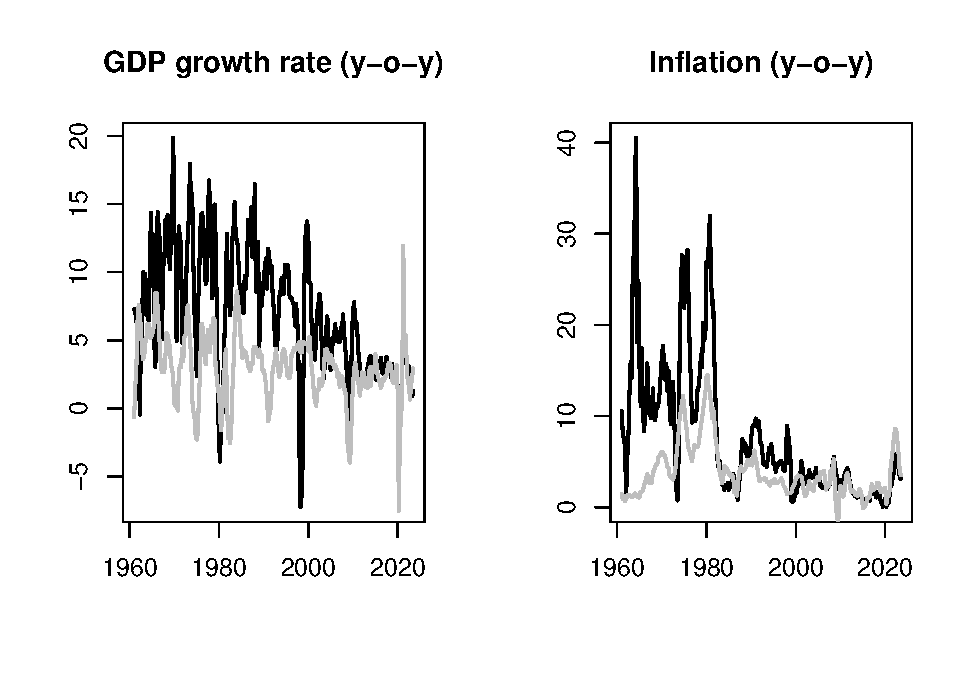
\includegraphics[width=0.95\linewidth]{IdentifStructShocks_files/figure-latex/VARdataUSAKOR-1} \caption{GDP log growth rates and inflation rates for the US and Korea. Black lines are for Korea; grey lines are for the US. All series are year-on-year growth rates, expressed in percent.}\label{fig:VARdataUSAKOR}
\end{figure}

Let us first estimate an unrestricted VAR(\(p\)) model using these data.

\begin{Shaded}
\begin{Highlighting}[]
\NormalTok{p }\OtherTok{\textless{}{-}} \DecValTok{4}
\NormalTok{estVAR }\OtherTok{\textless{}{-}} \FunctionTok{VAR}\NormalTok{(Y, }\AttributeTok{p =}\NormalTok{ p) }\CommentTok{\# estimate the VAR model}
\NormalTok{L0 }\OtherTok{\textless{}{-}} \FunctionTok{logLik}\NormalTok{(estVAR)}
\end{Highlighting}
\end{Shaded}

The model log-likelihood is stored in \texttt{L0}.

Let us now estimate a retricted model:

\begin{Shaded}
\begin{Highlighting}[]
\NormalTok{n }\OtherTok{\textless{}{-}} \FunctionTok{dim}\NormalTok{(Y)[}\DecValTok{2}\NormalTok{]}
\NormalTok{restrict }\OtherTok{\textless{}{-}} \FunctionTok{matrix}\NormalTok{(}\DecValTok{1}\NormalTok{,n,}\DecValTok{1}\SpecialCharTok{+}\NormalTok{p}\SpecialCharTok{*}\NormalTok{n) }\CommentTok{\# \textquotesingle{}restrict\textquotesingle{} specifies restrictions; last column = \textquotesingle{}c\textquotesingle{}.}
\ControlFlowTok{for}\NormalTok{(i }\ControlFlowTok{in} \DecValTok{1}\SpecialCharTok{:}\NormalTok{p)\{}
\NormalTok{  restrict[}\DecValTok{1}\SpecialCharTok{:}\NormalTok{(n}\SpecialCharTok{/}\DecValTok{2}\NormalTok{),(n}\SpecialCharTok{/}\DecValTok{2}\SpecialCharTok{+}\NormalTok{n}\SpecialCharTok{*}\NormalTok{(i}\DecValTok{{-}1}\NormalTok{)}\SpecialCharTok{+}\DecValTok{1}\NormalTok{)}\SpecialCharTok{:}\NormalTok{(i}\SpecialCharTok{*}\NormalTok{n)] }\OtherTok{\textless{}{-}} \DecValTok{0}
\NormalTok{\}}
\NormalTok{estVARrestr }\OtherTok{\textless{}{-}} \FunctionTok{restrict}\NormalTok{(estVAR, }\AttributeTok{method =} \StringTok{"man"}\NormalTok{, }\AttributeTok{resmat =}\NormalTok{ restrict)}
\NormalTok{Lrestr }\OtherTok{\textless{}{-}} \FunctionTok{logLik}\NormalTok{(estVARrestr)}
\end{Highlighting}
\end{Shaded}

The model log-likelihood is stored in \texttt{Lrestr}. We can perform a Likelihood Ratio (LR) test to see whether the data call for the exogeneity of the US variables. According to its definition (Def. \ref{def:LR}), the LR test statistics is given by:
\[
\xi^{LR} =2 \times (\hat{L} - \hat{L}^*), 
\]
where \(\hat{L}\) and \(\hat{L}^*\) are, respectively, the unrestricted and restricted maximum log-likelihoods. Under the null hypothesis that the block exogeneity is satisfied, we have:
\[
\xi^{LR} \sim \chi^2\left[p\left(\frac{n}{2}\right)^2\right].
\]

In our context, we can therefore apply the test as follows:

\begin{Shaded}
\begin{Highlighting}[]
\NormalTok{LRstat }\OtherTok{\textless{}{-}} \DecValTok{2}\SpecialCharTok{*}\NormalTok{(L0 }\SpecialCharTok{{-}}\NormalTok{ Lrestr)}
\NormalTok{df }\OtherTok{\textless{}{-}} \FunctionTok{length}\NormalTok{(restrict)}\SpecialCharTok{{-}}\FunctionTok{sum}\NormalTok{(restrict)}
\NormalTok{pvalue }\OtherTok{\textless{}{-}} \DecValTok{1} \SpecialCharTok{{-}} \FunctionTok{pchisq}\NormalTok{(LRstat,}\AttributeTok{df=}\NormalTok{df)}
\FunctionTok{print}\NormalTok{(}\FunctionTok{c}\NormalTok{(pvalue))}
\end{Highlighting}
\end{Shaded}

\begin{verbatim}
## [1] 0.3977775
\end{verbatim}

Hence, the test cannot reject the null hypothesis of block exogeneity since the p-value is larger than conventional thresholds. In terms or coding, we could have used, equivalently, the \texttt{lrtest} function to perform this test:

\begin{Shaded}
\begin{Highlighting}[]
\FunctionTok{lrtest}\NormalTok{(estVAR,estVARrestr)}
\end{Highlighting}
\end{Shaded}

\begin{verbatim}
## Likelihood ratio test
## 
## Model 1: VAR(y = Y, p = p)
## Model 2: VAR(y = Y, p = p)
##   #Df  LogLik  Df  Chisq Pr(>Chisq)
## 1  68 -1685.5                      
## 2  52 -1693.9 -16 16.813     0.3978
\end{verbatim}

Let us compare the IRFs in both models (w/ and w/o block exogeneity). In Figure \ref{fig:IRFblockexog}, the grey lines correspond to a contrained model, where Korean variables do not affect US ones. (In other words, in the restricted model, US variables are exogenous.) Notice that, in the restricted model, the last two shocks (\(\eta_{3,t}\) and \(\eta_{4,t}\)) do not affect US variables.

\begin{Shaded}
\begin{Highlighting}[]
\CommentTok{\# Unrestricted model:}
\NormalTok{Phi }\OtherTok{\textless{}{-}} \FunctionTok{Acoef}\NormalTok{(estVAR)}
\NormalTok{eps }\OtherTok{\textless{}{-}} \FunctionTok{residuals}\NormalTok{(estVAR)}
\NormalTok{Omega }\OtherTok{\textless{}{-}} \FunctionTok{var}\NormalTok{(eps) }\CommentTok{\# covariance matrix of OLS residuals}
\NormalTok{B }\OtherTok{\textless{}{-}} \FunctionTok{t}\NormalTok{(}\FunctionTok{chol}\NormalTok{(Omega)) }\CommentTok{\# Cholesky decomposition of Omega (lower triangular)}
\CommentTok{\# Restricted model:}
\NormalTok{Phi\_restr }\OtherTok{\textless{}{-}} \FunctionTok{Acoef}\NormalTok{(estVARrestr)}
\NormalTok{eps\_restr }\OtherTok{\textless{}{-}} \FunctionTok{residuals}\NormalTok{(estVARrestr)}
\NormalTok{Omega\_restr }\OtherTok{\textless{}{-}} \FunctionTok{var}\NormalTok{(eps\_restr)}
\NormalTok{B\_restr }\OtherTok{\textless{}{-}} \FunctionTok{t}\NormalTok{(}\FunctionTok{chol}\NormalTok{(Omega\_restr))}

\FunctionTok{par}\NormalTok{(}\AttributeTok{mfrow =} \FunctionTok{c}\NormalTok{(n, n))}
\FunctionTok{par}\NormalTok{(}\AttributeTok{plt =} \FunctionTok{c}\NormalTok{(.}\DecValTok{35}\NormalTok{, .}\DecValTok{97}\NormalTok{, .}\DecValTok{25}\NormalTok{, .}\DecValTok{68}\NormalTok{))}
\NormalTok{Model }\OtherTok{\textless{}{-}} \FunctionTok{list}\NormalTok{(}\AttributeTok{c =}\NormalTok{ c, }\AttributeTok{Phi =}\NormalTok{ Phi, }\AttributeTok{B =}\NormalTok{ B)}
\ControlFlowTok{for}\NormalTok{ (shock }\ControlFlowTok{in} \DecValTok{1}\SpecialCharTok{:}\NormalTok{n) \{}
\NormalTok{  eta0 }\OtherTok{\textless{}{-}} \FunctionTok{rep}\NormalTok{(}\DecValTok{0}\NormalTok{, n)}
\NormalTok{  eta0[shock] }\OtherTok{\textless{}{-}} \DecValTok{1}
\NormalTok{  res.sim }\OtherTok{\textless{}{-}} \FunctionTok{simul.VAR}\NormalTok{(}\AttributeTok{c =} \ConstantTok{NaN}\NormalTok{, Phi, B, }\AttributeTok{nb.sim =} \DecValTok{30}\NormalTok{, }\AttributeTok{indic.IRF =} \DecValTok{1}\NormalTok{,}
                       \AttributeTok{u.shock =}\NormalTok{ eta0)}
\NormalTok{  res.sim\_restr }\OtherTok{\textless{}{-}} \FunctionTok{simul.VAR}\NormalTok{(}\AttributeTok{c =} \ConstantTok{NaN}\NormalTok{, Phi\_restr, B\_restr, }\AttributeTok{nb.sim =} \DecValTok{30}\NormalTok{,}
                             \AttributeTok{indic.IRF =} \DecValTok{1}\NormalTok{,}\AttributeTok{u.shock =}\NormalTok{ eta0)}
  \ControlFlowTok{for}\NormalTok{ (variable }\ControlFlowTok{in} \DecValTok{1}\SpecialCharTok{:}\NormalTok{n) \{}
    \FunctionTok{plot}\NormalTok{(res.sim[, variable], }\AttributeTok{type =} \StringTok{"l"}\NormalTok{, }\AttributeTok{lwd =} \DecValTok{2}\NormalTok{, }\AttributeTok{las =} \DecValTok{1}\NormalTok{,}
         \AttributeTok{ylab =} \FunctionTok{ifelse}\NormalTok{(variable}\SpecialCharTok{==}\DecValTok{1}\NormalTok{,}
                       \FunctionTok{paste}\NormalTok{(}\StringTok{"Shock η"}\NormalTok{, shock, }\AttributeTok{sep =} \StringTok{""}\NormalTok{),}\StringTok{""}\NormalTok{),}\AttributeTok{xlab=}\StringTok{""}\NormalTok{,}
         \AttributeTok{main =} \FunctionTok{ifelse}\NormalTok{(shock}\SpecialCharTok{==}\DecValTok{1}\NormalTok{,}
                       \FunctionTok{paste}\NormalTok{(}\StringTok{"Resp. of "}\NormalTok{, names.var[variable],}\AttributeTok{sep =} \StringTok{""}\NormalTok{),}\StringTok{""}\NormalTok{))}
    \FunctionTok{lines}\NormalTok{(res.sim\_restr[, variable], }\AttributeTok{type =} \StringTok{"l"}\NormalTok{, }\AttributeTok{lwd =} \DecValTok{2}\NormalTok{,}\AttributeTok{col=}\StringTok{"grey"}\NormalTok{)}
\NormalTok{  \}}
\NormalTok{\}}
\end{Highlighting}
\end{Shaded}

\begin{figure}
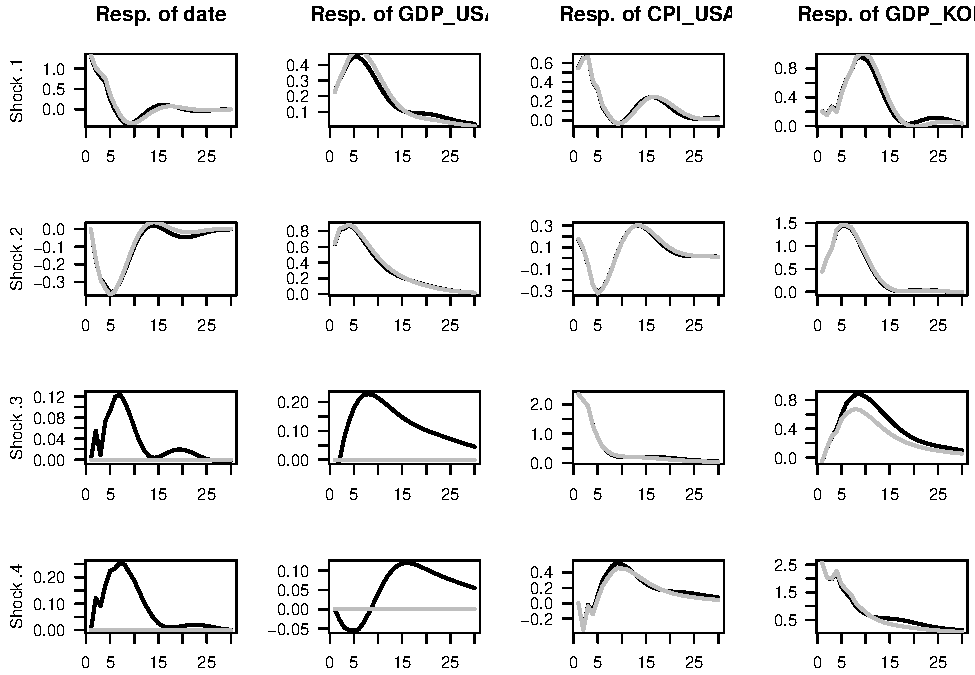
\includegraphics[width=0.95\linewidth]{IdentifStructShocks_files/figure-latex/IRFblockexog-1} \caption{Impulse response functions in the context of VAR models depicting the joint dynamics of US and Korean GDP growth and inflation rates. Structural shocks are identified by using the Cholesky decomposition. The grey lines correspond to a contrained model, where Korean variables do not affect US ones. (In other words, in the restricted model, US variables are exogenous.)}\label{fig:IRFblockexog}
\end{figure}

Finally, let us compute the variance decomposition in both models. Let us start with the unrestricted model:

\begin{Shaded}
\begin{Highlighting}[]
\FunctionTok{make\_variance\_decompo}\NormalTok{(Phi, B, }\AttributeTok{maxHorizon =} \DecValTok{50}\NormalTok{,}
                      \AttributeTok{names.var =} \FunctionTok{names}\NormalTok{(Y),}\AttributeTok{mfrow =} \FunctionTok{c}\NormalTok{(}\DecValTok{2}\NormalTok{,}\DecValTok{2}\NormalTok{))}
\end{Highlighting}
\end{Shaded}

\begin{figure}
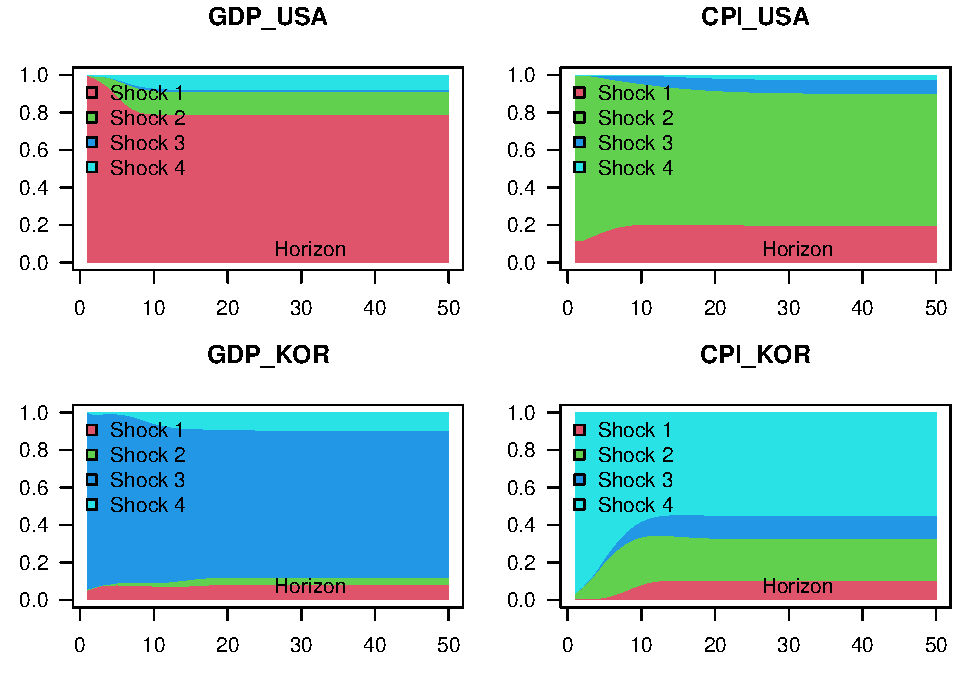
\includegraphics[width=0.95\linewidth]{IdentifStructShocks_files/figure-latex/VARdecblockexogUS-1} \caption{Variance decomposition in the context of a VAR model depicting the joint dynamics of US and Korean GDP growth and inflation rates. Structural shocks are identified by using the Cholesky decomposition. The grey lines correspond to a contrained model, where Korean variables do not affect US ones. (In other words, in the restricted model, US variables are exogenous.)}\label{fig:VARdecblockexogUS}
\end{figure}

Figure \ref{fig:VARdecblockexogCH} shows the variance decomposition in the context of the restricted model, that entails block exogeneity:

\begin{Shaded}
\begin{Highlighting}[]
\FunctionTok{make\_variance\_decompo}\NormalTok{(Phi\_restr, B\_restr, }\AttributeTok{maxHorizon =} \DecValTok{50}\NormalTok{,}
                      \AttributeTok{names.var =} \FunctionTok{names}\NormalTok{(Y),}\AttributeTok{mfrow =} \FunctionTok{c}\NormalTok{(}\DecValTok{2}\NormalTok{,}\DecValTok{2}\NormalTok{))}
\end{Highlighting}
\end{Shaded}

\begin{figure}
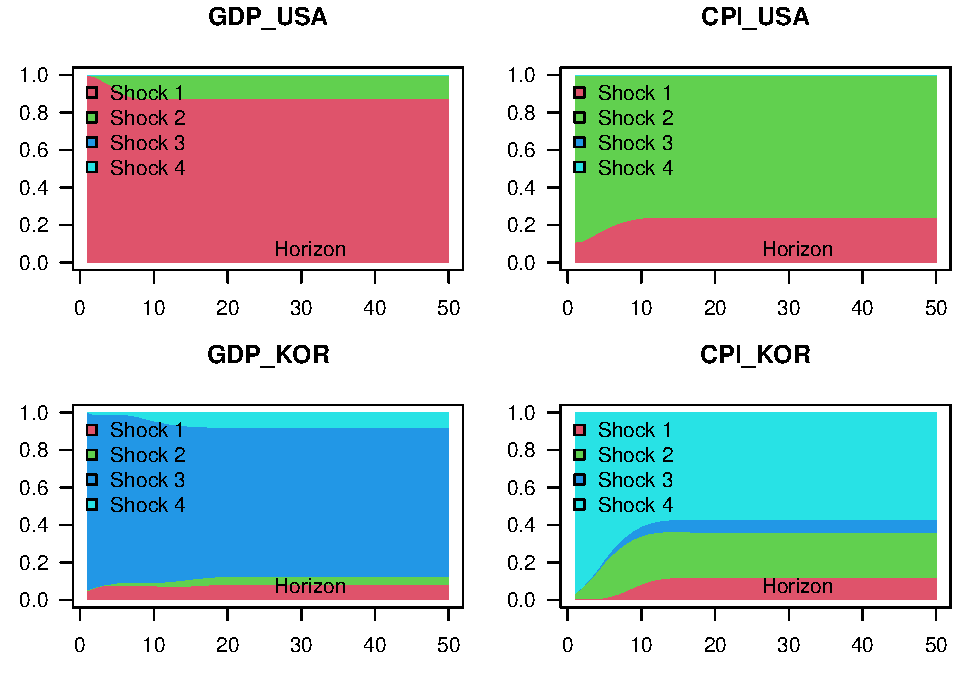
\includegraphics[width=0.95\linewidth]{IdentifStructShocks_files/figure-latex/VARdecblockexogCH-1} \caption{Variance decomposition in the context of a VAR model depicting the joint dynamics of US and Korean GDP growth and inflation rates. Structural shocks are identified by using the Cholesky decomposition. The model is contrained in such a way that Korean variables do not affect US ones. (In other words, in this restricted model, US variables are exogenous.)}\label{fig:VARdecblockexogCH}
\end{figure}

\subsection{Granger Causality}\label{granger-causality}

\citet{Granger_1969} developed a method to explore \textbf{causal relationships} among variables. The approach consists in determining whether the past values of \(y_{1,t}\) can help explain the current \(y_{2,t}\) (beyond the information already included in the past values of \(y_{2,t}\)).

Formally, let us denote three information sets:
\begin{eqnarray*}
\mathcal{I}_{1,t} & = & \left\{ y_{1,t},y_{1,t-1},\ldots\right\} \\
\mathcal{I}_{2,t} & = & \left\{ y_{2,t},y_{2,t-1},\ldots\right\} \\
\mathcal{I}_{t} & = & \left\{ y_{1,t},y_{1,t-1},\ldots y_{2,t},y_{2,t-1},\ldots\right\}.
\end{eqnarray*}
We say that \(y_{1,t}\) Granger-causes \(y_{2,t}\) if
\[
\mathbb{E}\left[y_{2,t}\mid \mathcal{I}_{2,t-1}\right]\neq \mathbb{E}\left[y_{2,t}\mid \mathcal{I}_{t-1}\right].
\]

To get the intuition behind the testing procedure, consider the following
bivariate VAR(\(p\)) process:
\begin{eqnarray*}
y_{1,t} & = & c_1+\Sigma_{i=1}^{p}\Phi_i^{(11)}y_{1,t-i}+\Sigma_{i=1}^{p}\Phi_i^{(12)}y_{2,t-i}+\varepsilon_{1,t}\\
y_{2,t} & = & c_2+\Sigma_{i=1}^{p}\Phi_i^{(21)}y_{1,t-i}+\Sigma_{i=1}^{p}\Phi_i^{(22)}y_{2,t-i}+\varepsilon_{2,t},
\end{eqnarray*}
where \(\Phi_k^{(ij)}\) denotes the element \((i,j)\) of \(\Phi_k\). Then, \(y_{1,t}\) is said not to Granger-cause \(y_{2,t}\) if
\[
\Phi_1^{(21)}=\Phi_2^{(21)}=\ldots=\Phi_p^{(21)}=0.
\]
The null and alternative hypotheses therefore are:
\[
\begin{cases}
H_{0}: & \Phi_1^{(21)}=\Phi_2^{(21)}=\ldots=\Phi_p^{(21)}=0\\
H_{1}: & \Phi_1^{(21)}\neq0\mbox{ or }\Phi_2^{(21)}\neq0\mbox{ or}\ldots\Phi_p^{(21)}\neq0.\end{cases}
\]
Loosely speaking, we reject \(H_{0}\) if some of the coefficients on the lagged \(y_{1,t}\)'s are statistically significant. Formally, this can be tested using the \(F\)-test or asymptotic chi-square test. The \(F\)-statistic is
\[
F=\frac{(RSS-USS)/p}{USS/(T-2p-1)},
\]
where RSS is the Restricted sum of squared residuals and USS is the Unrestricted sum of squared residuals. Under \(H_{0}\), the \(F\)-statistic is distributed as \(\mathcal{F}(p,T-2p-1)\) (See Table \ref{tab:Fstat}).\footnote{We have \(pF\underset{T \rightarrow \infty}{\rightarrow}\chi^{2}(p)\).}

According to the following lines of code, the output gap Granger-causes inflation, but the reverse is not true:

\begin{Shaded}
\begin{Highlighting}[]
\FunctionTok{grangertest}\NormalTok{(}\AttributeTok{x=}\FunctionTok{as.matrix}\NormalTok{(US3var[,}\FunctionTok{c}\NormalTok{(}\StringTok{"y.gdp.gap"}\NormalTok{,}\StringTok{"infl"}\NormalTok{)]),}\AttributeTok{order=}\DecValTok{3}\NormalTok{)}
\end{Highlighting}
\end{Shaded}

\begin{verbatim}
## Granger causality test
## 
## Model 1: infl ~ Lags(infl, 1:3) + Lags(y.gdp.gap, 1:3)
## Model 2: infl ~ Lags(infl, 1:3)
##   Res.Df Df      F   Pr(>F)   
## 1    214                      
## 2    217 -3 3.9761 0.008745 **
## ---
## Signif. codes:  0 '***' 0.001 '**' 0.01 '*' 0.05 '.' 0.1 ' ' 1
\end{verbatim}

\begin{Shaded}
\begin{Highlighting}[]
\FunctionTok{grangertest}\NormalTok{(}\AttributeTok{x=}\FunctionTok{as.matrix}\NormalTok{(US3var[,}\FunctionTok{c}\NormalTok{(}\StringTok{"infl"}\NormalTok{,}\StringTok{"y.gdp.gap"}\NormalTok{)]),}\AttributeTok{order=}\DecValTok{3}\NormalTok{)}
\end{Highlighting}
\end{Shaded}

\begin{verbatim}
## Granger causality test
## 
## Model 1: y.gdp.gap ~ Lags(y.gdp.gap, 1:3) + Lags(infl, 1:3)
## Model 2: y.gdp.gap ~ Lags(y.gdp.gap, 1:3)
##   Res.Df Df      F Pr(>F)
## 1    214                 
## 2    217 -3 1.5451 0.2038
\end{verbatim}

\chapter{Identification problem and standard identification techniques}\label{identifStruct}

\section{The identification problem}\label{IdentifPbm}

In Section \ref{estimVAR}, we have seen how to estimate \(\mathbb{V}ar(\varepsilon_t) =\Omega\) and the \(\Phi_k\) matrices in the context of a VAR model. But the IRFs are functions of \(B\) and of the \(\Phi_k\)'s, not of \(\Omega\) the \(\Phi_k\)'s (see Section \ref{IRFSVARMA}). We have \(\Omega = BB'\), which provides some restrictions on the components of \(B\), but this is not sufficient to fully identify \(B\). Indeed, seen a system of equations whose unknowns are the \(b_{i,j}\)'s (components of \(B\)), the system \(\Omega = BB'\) contains only \(n(n+1)/2\) linearly independent equations. For instance, for \(n=2\):
\begin{eqnarray*}
&&\left[
\begin{array}{cc}
\omega_{11} & \omega_{12} \\
\omega_{12} & \omega_{22}
\end{array}
\right] = \left[
\begin{array}{cc}
b_{11} & b_{12} \\
b_{21} & b_{22}
\end{array}
\right]\left[
\begin{array}{cc}
b_{11} & b_{21} \\
b_{12} & b_{22}
\end{array}
\right]\\
&\Leftrightarrow&\left[
\begin{array}{cc}
\omega_{11} & \omega_{12} \\
\omega_{12} & \omega_{22}
\end{array}
\right] = \left[
\begin{array}{cc}
b_{11}^2+b_{12}^2 & \color{red}{b_{11}b_{21}+b_{12}b_{22}} \\
\color{red}{b_{11}b_{21}+b_{12}b_{22}} & b_{22}^2 + b_{21}^2
\end{array}
\right].
\end{eqnarray*}

We then have 3 linearly independent equations but 4 unknowns. Therefore, \(B\) is not identified based on second-order moments. Additional restrictions are required to identify \(B\). This section covers two standard identification schemes: \textbf{short-run} and \textbf{long-run} restrictions.

\begin{enumerate}
\def\labelenumi{\arabic{enumi}.}
\tightlist
\item
  A \textbf{short-run restriction (SRR)} prevents a structural shock from affecting an endogenous variable contemporaneously.
\end{enumerate}

\begin{itemize}
\tightlist
\item
  It is easy to implement: the appropriate entries of \(B\) are set to 0.
\item
  A particular (popular) case is that of the \textbf{Cholesky, or recursive approach} (Sections \ref{Cholesky} and \ref{Cholesky1}).
\item
  Examples include \citet{BERNANKE198649}, \citet{Sims_1986}, \citet{Gali_1992}, \citet{RubioRamirez_et_al_2010}.
\end{itemize}

\begin{enumerate}
\def\labelenumi{\arabic{enumi}.}
\setcounter{enumi}{1}
\tightlist
\item
  A \textbf{long-run restriction (LRR)} prevents a structural shock from having a cumulative impact on one of the endogenous variables (Section \ref{LRrestr}).
\end{enumerate}

\begin{itemize}
\tightlist
\item
  Additional computations are required to implement this. One needs to compute the cumulative effect of one of the structural shocks \(u_{t}\) on one of the endogenous variable.
\item
  Examples include \citet{Blanchard_Quah_1989}, \citet{Faust_Leeper_1997}, \citet{Gali_1999}, \citet{Erceg_et_al_2005}, \citet{NBERc11177}.
\end{itemize}

As illustrated by Section \ref{Mixing}, the two approaches can be combined (see, e.g., \citet{Gerlach_Smets_1995}).

\section{A stylized example motivating short-run restrictions}\label{a-stylized-example-motivating-short-run-restrictions}

Let us consider a simple example that could motivate short-run restrictions. Consider the following stylized macro model:
\begin{equation}
\begin{array}{clll}
g_{t}&=& \bar{g}-\lambda(i_{t-1}-\mathbb{E}_{t-1}\pi_{t})+ \underbrace{{\color{blue}\sigma_d \eta_{d,t}}}_{\mbox{demand shock}}& (\mbox{IS curve})\\
\Delta \pi_{t} & = & \beta (g_{t} - \bar{g})+ \underbrace{{\color{blue}\sigma_{\pi} \eta_{\pi,t}}}_{\mbox{cost push shock}} & (\mbox{Phillips curve})\\
i_{t} & = & \rho i_{t-1} + \left[ \gamma_\pi \mathbb{E}_{t}\pi_{t+1}  + \gamma_g (g_{t} - \bar{g}) \right]\\
&& \qquad \qquad+\underbrace{{\color{blue}\sigma_{mp} \eta_{mp,t}}}_{\mbox{Mon. Pol. shock}} & (\mbox{Taylor rule}),
\end{array}\label{eq:systemI}
\end{equation}
where:
\begin{equation}
\eta_t = 
\left[
\begin{array}{c}
\eta_{\pi,t}\\
\eta_{d,t}\\
\eta_{mp,t}
\end{array}
\right]
\sim i.i.d.\,\mathcal{N}(0,I).\label{eq:covU}
\end{equation}

Vector \(\eta_t\) is assumed to be a vector of structural shocks, mutually and serially independent. On date \(t\):

\begin{itemize}
\tightlist
\item
  \(g_t\) is contemporaneously affected by \(\eta_{d,t}\) only;
\item
  \(\pi_t\) is contemporaneously affected by \(\eta_{\pi,t}\) and \(\eta_{d,t}\);
\item
  \(i_t\) is contemporaneously affected by \(\eta_{mp,t}\), \(\eta_{\pi,t}\) and \(\eta_{d,t}\).
\end{itemize}

System \eqref{eq:systemI} could be rewritten as follows:
\begin{equation}
\left[\begin{array}{c}
g_t\\
\pi_t\\
i_t
\end{array}\right]
= \Phi(L)
\left[\begin{array}{c}
g_{t-1}\\
\pi_{t-1}\\
i_{t-1} +
\end{array}\right] +\underbrace{\underbrace{
\left[
\begin{array}{ccc}
0 & \bullet & 0 \\
\bullet & \bullet & 0 \\
\bullet & \bullet & \bullet
\end{array}
\right]}_{=B} \eta_t.}_{=\varepsilon_t}\label{eq:BBBB}
\end{equation}

This is the \textbf{reduced-form} of the model. This representation suggests three additional restrictions on the entries of \(B\); the latter matrix is therefore identified as soon as \(\Omega = BB'\) is known (up to the signs of its columns).

\section{Cholesky: a specific short-run-restriction situation}\label{Cholesky}

There are particular cases in which some well-known matrix decomposition of \(\Omega=\mathbb{V}ar(\varepsilon_t)\) can be used to easily estimate some specific SVAR. This is the case for the so-called Cholesky decomposition. Consider the following context:

\begin{itemize}
\tightlist
\item
  A first shock (say, \(\eta_{n_1,t}\)) can affect instantaneously
  (i.e., on date \(t\)) only one of the endogenous variable (say, \(y_{n_1,t}\));
\item
  A second shock (say, \(\eta_{n_2,t}\)) can affect instantaneously
  (i.e., on date \(t\)) two endogenous variables, \(y_{n_1,t}\) (the same as before) and \(y_{n_2,t}\);
\item
  \(\dots\)
\end{itemize}

This implies

\begin{enumerate}
\def\labelenumi{\arabic{enumi}.}
\tightlist
\item
  that column \(n_1\) of \(B\) has only 1 non-zero entry (this is the \(n_1^{th}\) entry),
\item
  that column \(n_2\) of \(B\) has 2 non-zero entries (the \(n_1^{th}\) and the \(n_2^{th}\) ones), etc.
\end{enumerate}

Without loss of generality, we can set \(n_1=n\), \(n_2=n-1\), etc. In this context, matrix \(B\) is lower triangular. The Cholesky decomposition of \(\Omega_{\varepsilon}\) then provides an appropriate estimate of \(B\), since this matrix decomposition yields to a lower triangular matrix satisfying:
\[
\Omega_\varepsilon = BB'.
\]

For instance, \citet{DEDOLA20051543} estimate 5 structural VAR models for the US, the UK, Germany, France and Italy to analyse the monetary-policy transmission mechanisms. They estimate SVAR(5) models over the period 1975-1997. The shock-identification scheme is based on Cholesky decompositions, the ordering of the endogenous variables being: (1) the industrial production, (2) the consumer price index, (3) a commodity price index, (4) the short-term rate, (5) monetary aggregate and (6) the effective exchange rate (except for the US). This ordering implies that monetary policy (i.e., the short-term rate) reacts to the shocks affecting the first three variables but that the latter react to monetary policy shocks with a one-period lag only.

Consider again the small structural example discussed above, whose reduced-form VAR representation is given in Eq. \eqref{eq:BBBB}. If we reorder the structural shocks as \(\eta_t = (\eta_{d,t},\eta_{\pi,t},\eta_{mp,t})'\) (the order being arbitrary), the impact matrix \(B\) can be written as
\[
B = \begin{bmatrix}
\bullet & 0 & 0 \\
\bullet & \bullet & 0 \\
\bullet & \bullet & \bullet
\end{bmatrix},
\]
that is, \(B\) corresponds to the Cholesky factor of \(\Omega\).

However, it is not always possible to obtain a lower-triangular \(B\) matrix by reordering the structural shocks. For instance, if for a given ordering we have
\[
B = \begin{bmatrix}
0 & \bullet & \bullet \\
\bullet & 0 & \bullet \\
\bullet & \bullet & 0
\end{bmatrix},
\]
then no reordering of the shocks will produce a lower-triangular structure.

The Cholesky approach has been used in the previous chapter, in Example \ref{exm:US3varselect} (see Figure \ref{fig:US3varIRFs1}).

\section{Using Cholesky to identify a single shock}\label{Cholesky1}

In some cases, the Cholesky approach can be employed when interest centers on a single structural shock. This is the case, for example, in \citet{Christiano_Eichenbaum_Evans_1996}. Their identification is based on the following relationship between \(\varepsilon_t\) and \(\eta_t\):
\begin{equation}
\left[\begin{array}{c}
\boldsymbol\varepsilon_{S,t}\\
\varepsilon_{r,t}\\
\boldsymbol\varepsilon_{F,t}
\end{array}\right] =
\left[\begin{array}{ccc}
B_{SS} & 0 & 0 \\
B_{rS} & B_{rr} & 0 \\
B_{FS} & B_{Fr} & B_{FF}
\end{array}\right]
\left[\begin{array}{c}
\boldsymbol\eta_{S,t}\\
\eta_{r,t}\\
\boldsymbol\eta_{F,t}
\end{array}\right],\label{eq:BCEE}
\end{equation}
where \(S\), \(r\) and \(F\) respectively correspond to \emph{slow-moving variables}, the policy variable (short-term rate) and \emph{fast-moving variables}. While \(\eta_{r,t}\) is scalar, \(\boldsymbol\eta_{S,t}\) and \(\boldsymbol\eta_{F,t}\) may be vectors. The space spanned by \(\boldsymbol\varepsilon_{S,t}\) is the same as that spanned by \(\boldsymbol\eta_{S,t}\). As a result, because \(\varepsilon_{r,t}\) is a linear combination of \(\eta_{r,t}\) and \(\boldsymbol\eta_{S,t}\) (which are \(\perp\)), it comes that the \(B_{rr}\eta_{r,t}\)'s are the (population) residuals in the regression of \(\varepsilon_{r,t}\) on \(\boldsymbol\varepsilon_{S,t}\). Because \(\mathbb{V}ar(\eta_{r,t})=1\), \(B_{rr}\) is given by the square root of the variance of \(B_{rr}\eta_{r,t}\). \(B_{F,r}\) is finally obtained by regressing the components of \(\boldsymbol\varepsilon_{F,t}\) on the estimates of \(\eta_{r,t}\).

A critical observation is that all matrices \(B\) with the block form in Eq. (\citet{ref}(eq:BCEE)) (with \(B_{rr}>0\)) and satisfying \(\Omega=BB'\) share the same intermediate column (that is, the same \(B_{rr}\) and \(B_{Fr}\)). One such \(B\) is obtained directly from the Cholesky decomposition of \(\Omega=BB'\).

\begin{Shaded}
\begin{Highlighting}[]
\FunctionTok{library}\NormalTok{(IdSS)}
\FunctionTok{library}\NormalTok{(vars)}
\FunctionTok{data}\NormalTok{(}\StringTok{"USmonthly"}\NormalTok{)}
\CommentTok{\# Select sample period:}
\NormalTok{First.date }\OtherTok{\textless{}{-}} \StringTok{"1965{-}01{-}01"}\NormalTok{;Last.date }\OtherTok{\textless{}{-}} \StringTok{"1995{-}06{-}01"}
\NormalTok{indic.first }\OtherTok{\textless{}{-}} \FunctionTok{which}\NormalTok{(USmonthly}\SpecialCharTok{$}\NormalTok{DATES}\SpecialCharTok{==}\NormalTok{First.date)}
\NormalTok{indic.last  }\OtherTok{\textless{}{-}} \FunctionTok{which}\NormalTok{(USmonthly}\SpecialCharTok{$}\NormalTok{DATES}\SpecialCharTok{==}\NormalTok{Last.date)}
\NormalTok{USmonthly   }\OtherTok{\textless{}{-}}\NormalTok{ USmonthly[indic.first}\SpecialCharTok{:}\NormalTok{indic.last,]}
\NormalTok{considered.variables }\OtherTok{\textless{}{-}} \FunctionTok{c}\NormalTok{(}\StringTok{"LIP"}\NormalTok{,}\StringTok{"UNEMP"}\NormalTok{,}\StringTok{"LCPI"}\NormalTok{,}\StringTok{"LPCOM"}\NormalTok{,}\StringTok{"FFR"}\NormalTok{,}\StringTok{"NBR"}\NormalTok{,}\StringTok{"TTR"}\NormalTok{,}\StringTok{"M1"}\NormalTok{)}
\NormalTok{y }\OtherTok{\textless{}{-}} \FunctionTok{as.matrix}\NormalTok{(USmonthly[considered.variables])}
\NormalTok{res.svar.ordering }\OtherTok{\textless{}{-}} \FunctionTok{svar.ordering}\NormalTok{(y,}\AttributeTok{p=}\DecValTok{3}\NormalTok{,}
                                   \AttributeTok{posit.of.shock =} \DecValTok{5}\NormalTok{,}
                                   \AttributeTok{nb.periods.IRF =} \DecValTok{20}\NormalTok{,}
                                   \AttributeTok{nb.bootstrap.replications =} \DecValTok{100}\NormalTok{,}
                                   \AttributeTok{confidence.interval =} \FloatTok{0.90}\NormalTok{, }\CommentTok{\# expressed in pp.}
                                   \AttributeTok{indic.plot =} \DecValTok{1} \CommentTok{\# Plots are displayed if = 1.}
\NormalTok{                                   )}
\end{Highlighting}
\end{Shaded}

\begin{figure}
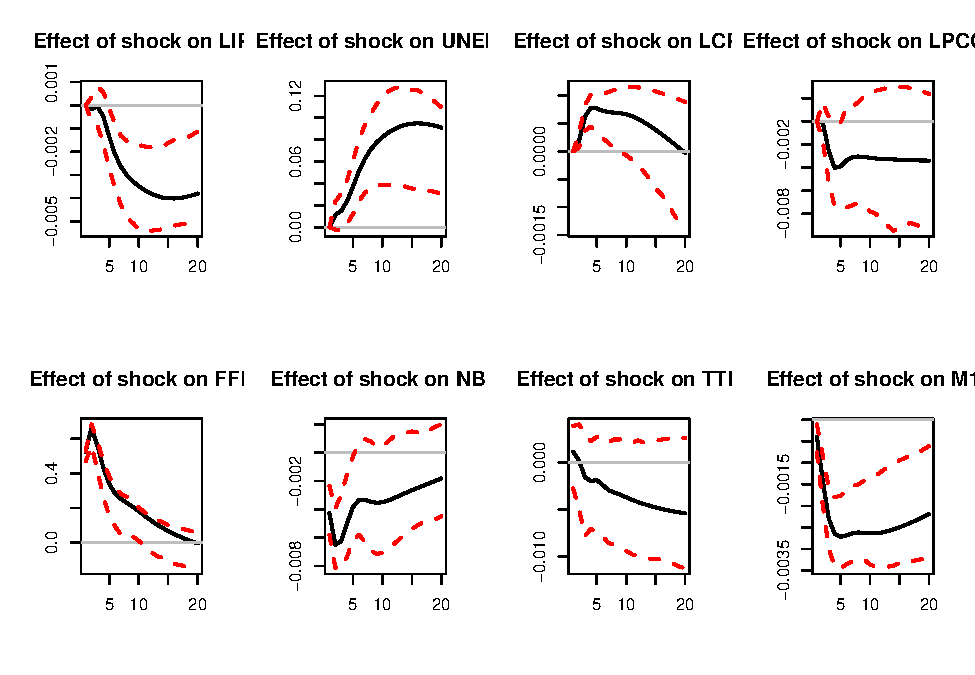
\includegraphics[width=0.95\linewidth]{IdentifStructShocks_files/figure-latex/CEE-1} \caption{Response to a monetary-policy shock. Identification approach of Christiano, Eichenbaum and Evans (1996). Confidence intervals are obtained by boostrapping the estimated VAR model (see inference section).}\label{fig:CEE}
\end{figure}

\section{Long-run restrictions}\label{LRrestr}

Let us now turn to \textbf{long-run restrictions}. Such a restriction concerns the long-run influence of a shock on an endogenous variable. Let us consider for instance a structural shock that is assumed to have no ``long-run influence'' on GDP. How to express this? The long-run change in GDP can be expressed as \(GDP_{t+h} - GDP_t\), with \(h\) large. Note further that:
\[
GDP_{t+h} - GDP_t = \Delta GDP_{t+h} +\Delta GDP_{t+h-1} + \dots + \Delta GDP_{t+1}.
\]
Hence, the fact that a given structural shock (\(\eta_{i,t}\), say) has no long-run influence on GDP means that
\[
\lim_{h\rightarrow\infty}\frac{\partial GDP_{t+h}}{\partial \eta_{i,t}} = \lim_{h\rightarrow\infty} \frac{\partial}{\partial \eta_{i,t}}\left(\sum_{k=1}^h \Delta  GDP_{t+k}\right)= 0.
\]

As shown in the following sections, this long-run effect can be formulated as a function of \(B\) and of the matrices \(\Phi_i\) when \(y_t\) (including \(\Delta GDP_t\)) follows a VAR process.

\subsection{The VAR(1) case}\label{the-var1-case}

Let us start with the VAR(1) case. We have:
\begin{eqnarray*}
y_{t} &=& c+\Phi y_{t-1}+\varepsilon_{t}\\
& = & c+\varepsilon_{t}+\Phi(c+\varepsilon_{t-1})+\ldots+\Phi^{k}(c+\varepsilon_{t-k})+\ldots \\
& = & \mu +\varepsilon_{t}+\Phi\varepsilon_{t-1}+\ldots+\Phi^{k}\varepsilon_{t-k}+\ldots \\
& = & \mu +B\eta_{t}+\Phi B\eta_{t-1}+\ldots+\Phi^{k}B\eta_{t-k}+\ldots,
\end{eqnarray*}
which is the Wold representation of \(y_t\).

The sequence of shocks \(\{\eta_t\}\) determines the sequence \(\{y_t\}\). What if \(\{\eta_t\}\) is replaced with \(\{\tilde{\eta}_t\}\), where \(\tilde{\eta}_t=\eta_t\) if \(t \ne s\) and \(\tilde{\eta}_s=\eta_s + \gamma\)? Assume \(\{\tilde{y}_t\}\) is the associated ``perturbated'' sequence. We have \(\tilde{y}_t = y_t\) if \(t<s\). For \(t \ge s\), the Wold decomposition of \(\{\tilde{y}_t\}\) implies:
\[
\tilde{y}_t = y_t + \Phi^{t-s} B \gamma.
\]
Therefore, the cumulative impact of \(\gamma\) on \(\tilde{y}_t\) will be (for \(t \ge s\)):
\begin{eqnarray}
(\tilde{y}_t - y_t) +  (\tilde{y}_{t-1} - y_{t-1}) + \dots +  (\tilde{y}_s - y_s) &=& \nonumber \\
(Id + \Phi + \Phi^2 + \dots + \Phi^{t-s}) B \gamma.&& \label{eq:cumul}
\end{eqnarray}

Consider a shock on \(\eta_{1,t}\), with a magnitude of \(1\). This shock corresponds to \(\gamma = [1,0,\dots,0]'\). Given Eq. \eqref{eq:cumul}, the long-run cumulative effect of this shock on the endogenous variables is given by:
\[
\underbrace{\underbrace{(Id+\Phi+\ldots+\Phi^{k}+\ldots)}_{=(Id - \Phi)^{-1}}B}_{=: \Theta}\left[\begin{array}{c}
1\\
0\\
\vdots\\
0\end{array}\right],
\]
which is the first column of the \(n \times n\) matrix \(\Theta := (Id - \Phi)^{-1}B\).

In this context, consider the following long-run restriction: \emph{``the \(j^{th}\) structural shock has no cumulative impact on the \(i^{th}\) endogenous variable''}. It is equivalent to
\[
\Theta_{ij}=0,
\]
where \(\Theta_{ij}\) is the element \((i,j)\) of \(\Theta\).

If \(n(n-1)/2\) restrictions of this type can be made, then \(B\) is identified. In particular, in the case case where \(\Theta\) is lower-triangular, the problem admits an analytical solution. Indeed, let \(J = (I - \Phi)^{-1}\) (assumed to be invertible). We want \(\Theta = JB\) to be lower triangular and \(\Omega = BB'\). Since \(B = J^{-1} \Theta\), we have
\[
\Omega = BB' = J^{-1} \Theta \Theta' (J^{-1})' \;\Rightarrow\; J\Omega J' = \Theta \Theta'.
\]
Since \(\Omega\) is positive definite and \(J\) is invertible, \(\Sigma = J\Omega J'\) is positive definite. Take the (unique, with positive diagonal) Cholesky factorization \(\Sigma = \Theta \Theta'\) with \(\Theta\) lower triangular. Then set \(B = J^{-1} \Theta\). This \(B\) satisfies \(\Omega = BB'\) and \((I - \Phi)^{-1}B = \Theta\) is lower triangular.

\subsection{\texorpdfstring{The VAR(\(p\)) case}{The VAR(p) case}}\label{the-varp-case}

Several of the developments made above are still valid in the VAR(\(p\)) case since a VAR(\(p\)) process can be rewritten as a VAR(1) process by augmenting the state vector. More specifically, stack the last \(p\) values of vector \(y_t\) in vector \(y_{t}^{*}=[y_t',\dots,y_{t-p+1}']'\); Eq. \eqref{eq:yVAR} can then be rewritten in its \textbf{companion form}:
\begin{equation}
y_{t}^{*} =
\underbrace{\left[\begin{array}{c}
c\\
0_{n \times 1}\\
\vdots\\
0_{n \times 1}\end{array}\right]}_{=c^*}+
\underbrace{\left[\begin{array}{cccc}
\Phi_{1} & \Phi_{2} & \cdots & \Phi_{p}\\
I & 0 & \cdots & 0\\
0 & \ddots & 0 & 0\\
0 & 0 & I & 0\end{array}\right]}_{=\Phi}
y_{t-1}^{*}+
\underbrace{\left[\begin{array}{c}
\varepsilon_{t}\\
0_{n \times 1}\\
\vdots\\
0_{n \times 1}\end{array}\right]}_{\varepsilon_t^*},\label{eq:ystarVAR}
\end{equation}
where matrices \(\Phi\) and \(\Omega^*:= \mathbb{V}ar(\varepsilon_t^*)\) are of dimension \(np \times np\). Matrix \(\Phi\) had been introduced in Eq. \eqref{eq:matrixPHI}, and
\[
\Omega^* := \mathbb{V}ar(\varepsilon_t^*)=
\left[\begin{array}{c}
B \\
0_{n \times n}  \\
\vdots \\
0_{n \times n}
\end{array}\right]\left[\begin{array}{cccc}
B & 0_{n \times n} & \dots & 0_{n \times n}
\end{array}\right]
= \left[\begin{array}{cccc}
\Omega & 0_{n \times n} & \dots & 0_{n \times n} \\
0_{n \times n} & 0_{n \times n} \\
\vdots &&\ddots\\
0_{n \times n} & \dots &&0_{n \times n}
\end{array}\right].
\]
In that context, the long-run effect on \(y_t^*+y_{t+1}^*+y_{t+2}^*+\dots\) of a change in \(\eta_t\) by \(\gamma\) (that happens on date \(t\)) is given by:
\[
\underbrace{(Id+\Phi+\ldots+\Phi^{k}+\ldots)}_{=(Id - \Phi)^{-1}}\left[\begin{array}{c}
B \\
0_{n \times n}  \\
\vdots \\
0_{n \times n}
\end{array}\right]\gamma.
\]
In particular, the cumulated effect of this shock on \(y_t\) (and not \(y_t^*\) anymore) is \(J B \gamma\), where \(J\) is the upper-left \(n \times n\) submatrix of \((I - \Phi)^{-1}\). Let us denote the matrix \(J B\) by \(\Theta\). With these notations, the long-run restriction: \emph{the \(j^{th}\) structural shock has no cumulative impact on the \(i^{th}\) endogenous variable} is equivalent to the fact that the component \((i,j)\) of \(\Theta\) is equal to zero.

If \(n(n-1)/2\) restrictions of this type can be made, then \(B\) is identified. In particular, in the case where \(\Theta\) is lower triangular, the problem admits an analytical solution. Using \(B = J^{-1} \Theta\), we get
\[
\Omega = B B' = J^{-1} \Theta \Theta' (J^{-1})' \;\Rightarrow\; J \Omega J' = \Theta \Theta'.
\]
Since \(\Omega\) is positive definite, \(\Sigma = J \Omega J'\) is positive definite. Take the (unique, with positive diagonal) Cholesky factorization \(\Sigma = \Theta \Theta'\) with \(\Theta\) lower triangular. Then set \(B = J^{-1} \Theta\). This \(B\) satisfies \(\Omega = B B'\) and \(J B = \Theta\) is lower triangular.

\subsection{Blanchard and Quah (1989)}\label{blanchard-and-quah-1989}

\citet{Blanchard_Quah_1989} have implemented such long-run restrictions in a small-scale VAR. Two variables are considered: GDP and unemployment. Consequently, the VAR is affected by two types of shocks. Specifically, authors want to identify \textbf{supply shocks} (that can have a permanent effect on output) and \textbf{demand shocks} (that cannot have a permanent effect on output).\footnote{The motivation of the authors regarding their long-run restrictions can be obtained from a traditional Keynesian view of fluctuations. The authors propose a variant of a model from \citet{Fischer_1977}.
}

\citet{Blanchard_Quah_1989}'s dataset is quarterly, spanning the period from 1950:2 to 1987:4. Their VAR features 8 lags. Here are the data they use:

\begin{Shaded}
\begin{Highlighting}[]
\FunctionTok{library}\NormalTok{(IdSS)}
\FunctionTok{data}\NormalTok{(BQ)}
\FunctionTok{par}\NormalTok{(}\AttributeTok{mfrow=}\FunctionTok{c}\NormalTok{(}\DecValTok{1}\NormalTok{,}\DecValTok{2}\NormalTok{))}
\FunctionTok{plot}\NormalTok{(BQ}\SpecialCharTok{$}\NormalTok{Date,BQ}\SpecialCharTok{$}\NormalTok{Dgdp,}\AttributeTok{type=}\StringTok{"l"}\NormalTok{,}\AttributeTok{main=}\StringTok{"GDP quarterly growth rate"}\NormalTok{,}
     \AttributeTok{xlab=}\StringTok{""}\NormalTok{,}\AttributeTok{ylab=}\StringTok{""}\NormalTok{,}\AttributeTok{lwd=}\DecValTok{2}\NormalTok{)}
\FunctionTok{plot}\NormalTok{(BQ}\SpecialCharTok{$}\NormalTok{Date,BQ}\SpecialCharTok{$}\NormalTok{unemp,}\AttributeTok{type=}\StringTok{"l"}\NormalTok{,}\AttributeTok{ylim=}\FunctionTok{c}\NormalTok{(}\SpecialCharTok{{-}}\DecValTok{3}\NormalTok{,}\DecValTok{6}\NormalTok{),}\AttributeTok{main=}\StringTok{"Unemployment rate (gap)"}\NormalTok{,}
     \AttributeTok{xlab=}\StringTok{""}\NormalTok{,}\AttributeTok{ylab=}\StringTok{""}\NormalTok{,}\AttributeTok{lwd=}\DecValTok{2}\NormalTok{)}
\end{Highlighting}
\end{Shaded}

\begin{figure}
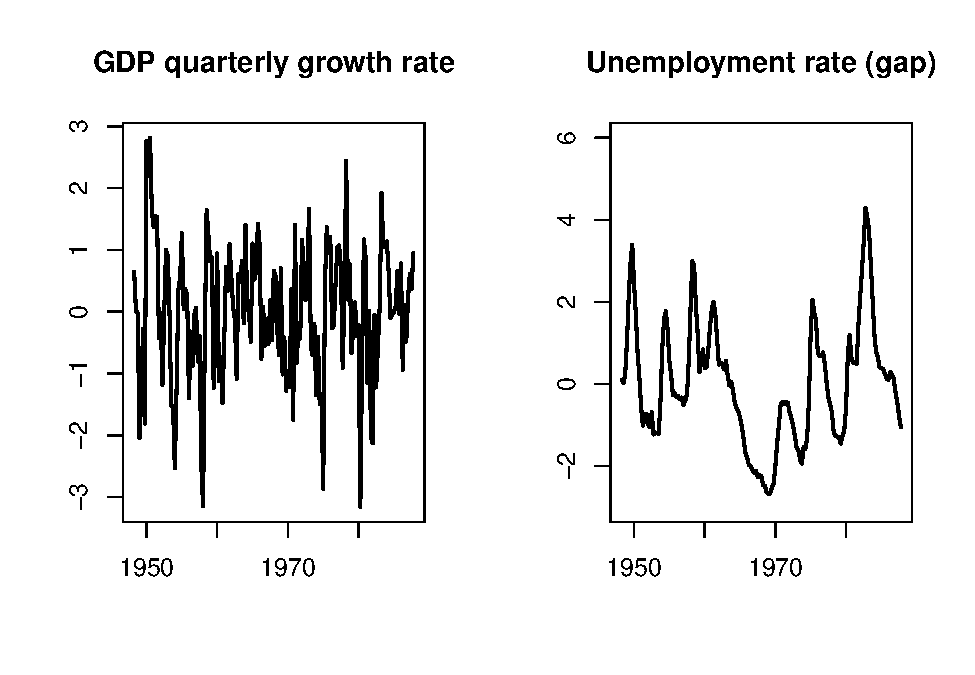
\includegraphics[width=0.95\linewidth]{IdentifStructShocks_files/figure-latex/BQ1-1} \caption{These data come from Blanchard and Quah (1989). GDP growth rates are calculated as the first differences of the logarithm of GDP.}\label{fig:BQ1}
\end{figure}

Estimate a reduced-form VAR(8) model:

\begin{Shaded}
\begin{Highlighting}[]
\FunctionTok{library}\NormalTok{(vars)}
\NormalTok{y }\OtherTok{\textless{}{-}}\NormalTok{ BQ[,}\DecValTok{2}\SpecialCharTok{:}\DecValTok{3}\NormalTok{]}
\NormalTok{n }\OtherTok{\textless{}{-}} \FunctionTok{dim}\NormalTok{(y)[}\DecValTok{2}\NormalTok{]}
\NormalTok{p }\OtherTok{\textless{}{-}} \DecValTok{8}
\NormalTok{est.VAR }\OtherTok{\textless{}{-}} \FunctionTok{VAR}\NormalTok{(y,}\AttributeTok{p=}\NormalTok{p)}
\NormalTok{Omega }\OtherTok{\textless{}{-}} \FunctionTok{var}\NormalTok{(}\FunctionTok{residuals}\NormalTok{(est.VAR))}
\end{Highlighting}
\end{Shaded}

Let us employ the approach described above:

\begin{Shaded}
\begin{Highlighting}[]
\NormalTok{Phi }\OtherTok{\textless{}{-}} \FunctionTok{Acoef}\NormalTok{(est.VAR)}
\NormalTok{PHI }\OtherTok{\textless{}{-}} \FunctionTok{make.PHI}\NormalTok{(Phi)}
\NormalTok{A }\OtherTok{\textless{}{-}} \FunctionTok{diag}\NormalTok{(n}\SpecialCharTok{*}\NormalTok{p) }\SpecialCharTok{{-}}\NormalTok{ PHI}
\NormalTok{J }\OtherTok{\textless{}{-}} \FunctionTok{solve}\NormalTok{(A)[}\DecValTok{1}\SpecialCharTok{:}\NormalTok{n,}\DecValTok{1}\SpecialCharTok{:}\NormalTok{n]}
\NormalTok{Sigma }\OtherTok{\textless{}{-}}\NormalTok{ J }\SpecialCharTok{\%*\%}\NormalTok{ Omega }\SpecialCharTok{\%*\%} \FunctionTok{t}\NormalTok{(J)}
\NormalTok{L }\OtherTok{\textless{}{-}} \FunctionTok{t}\NormalTok{(}\FunctionTok{chol}\NormalTok{(Sigma))}
\NormalTok{B }\OtherTok{\textless{}{-}} \FunctionTok{solve}\NormalTok{(J) }\SpecialCharTok{\%*\%}\NormalTok{ L}
\FunctionTok{print}\NormalTok{(B)}
\end{Highlighting}
\end{Shaded}

\begin{verbatim}
##           [,1]       [,2]
## [1,] 0.1541392 -0.8570365
## [2,] 0.1921245  0.2396346
\end{verbatim}

Alternatively, one may adopt a numerical approach by defining a loss function (\texttt{loss}) that equals zero when both conditions are satisfied: (a) \(BB' = \Omega\), and (b) the \((1,1)\) element of \(\Theta = (I - \Phi)^{-1}B\) is equal to zero.

\begin{Shaded}
\begin{Highlighting}[]
\CommentTok{\# Compute (Id {-} Phi)\^{}\{{-}1\}:}
\NormalTok{Phi }\OtherTok{\textless{}{-}} \FunctionTok{Acoef}\NormalTok{(est.VAR)}
\NormalTok{PHI }\OtherTok{\textless{}{-}} \FunctionTok{make.PHI}\NormalTok{(Phi)}
\NormalTok{sum.PHI.k }\OtherTok{\textless{}{-}} \FunctionTok{solve}\NormalTok{(}\FunctionTok{diag}\NormalTok{(}\FunctionTok{dim}\NormalTok{(PHI)[}\DecValTok{1}\NormalTok{]) }\SpecialCharTok{{-}}\NormalTok{ PHI)[}\DecValTok{1}\SpecialCharTok{:}\DecValTok{2}\NormalTok{,}\DecValTok{1}\SpecialCharTok{:}\DecValTok{2}\NormalTok{]}
\NormalTok{loss }\OtherTok{\textless{}{-}} \ControlFlowTok{function}\NormalTok{(param)\{}
\NormalTok{  B }\OtherTok{\textless{}{-}} \FunctionTok{matrix}\NormalTok{(param,}\DecValTok{2}\NormalTok{,}\DecValTok{2}\NormalTok{)}
\NormalTok{  X }\OtherTok{\textless{}{-}}\NormalTok{ Omega }\SpecialCharTok{{-}}\NormalTok{ B }\SpecialCharTok{\%*\%} \FunctionTok{t}\NormalTok{(B)}
\NormalTok{  Theta }\OtherTok{\textless{}{-}}\NormalTok{ sum.PHI.k[}\DecValTok{1}\SpecialCharTok{:}\DecValTok{2}\NormalTok{,}\DecValTok{1}\SpecialCharTok{:}\DecValTok{2}\NormalTok{] }\SpecialCharTok{\%*\%}\NormalTok{ B}
\NormalTok{  loss }\OtherTok{\textless{}{-}} \DecValTok{10000} \SpecialCharTok{*}\NormalTok{ ( X[}\DecValTok{1}\NormalTok{,}\DecValTok{1}\NormalTok{]}\SpecialCharTok{\^{}}\DecValTok{2} \SpecialCharTok{+}\NormalTok{ X[}\DecValTok{2}\NormalTok{,}\DecValTok{1}\NormalTok{]}\SpecialCharTok{\^{}}\DecValTok{2} \SpecialCharTok{+}\NormalTok{ X[}\DecValTok{2}\NormalTok{,}\DecValTok{2}\NormalTok{]}\SpecialCharTok{\^{}}\DecValTok{2} \SpecialCharTok{+}\NormalTok{ Theta[}\DecValTok{1}\NormalTok{,}\DecValTok{1}\NormalTok{]}\SpecialCharTok{\^{}}\DecValTok{2}\NormalTok{ )}
  \FunctionTok{return}\NormalTok{(loss)}
\NormalTok{\}}
\NormalTok{res.opt }\OtherTok{\textless{}{-}} \FunctionTok{optim}\NormalTok{(}\FunctionTok{c}\NormalTok{(}\DecValTok{1}\NormalTok{,}\DecValTok{0}\NormalTok{,}\DecValTok{0}\NormalTok{,}\DecValTok{1}\NormalTok{),loss,}\AttributeTok{method=}\StringTok{"BFGS"}\NormalTok{,}\AttributeTok{hessian=}\ConstantTok{FALSE}\NormalTok{)}
\FunctionTok{print}\NormalTok{(res.opt}\SpecialCharTok{$}\NormalTok{par)}
\end{Highlighting}
\end{Shaded}

\begin{verbatim}
## [1]  0.8570358 -0.2396345  0.1541395  0.1921221
\end{verbatim}

(Note: one can use that type of approach, based on a loss function, to mix short- and long-run restrictions.)

Figure \ref{fig:BQ4} displays the resulting IRFs. Note that, for GDP, we cumulate the GDP growth IRF, so as to have the response of the GDP in level.

\begin{Shaded}
\begin{Highlighting}[]
\NormalTok{B.hat }\OtherTok{\textless{}{-}} \FunctionTok{matrix}\NormalTok{(res.opt}\SpecialCharTok{$}\NormalTok{par,}\DecValTok{2}\NormalTok{,}\DecValTok{2}\NormalTok{)}
\FunctionTok{print}\NormalTok{(}\FunctionTok{cbind}\NormalTok{(Omega,B.hat }\SpecialCharTok{\%*\%} \FunctionTok{t}\NormalTok{(B.hat)))}
\end{Highlighting}
\end{Shaded}

\begin{verbatim}
##             Dgdp       unemp                       
## Dgdp   0.7582704 -0.17576173  0.7582694 -0.17576173
## unemp -0.1757617  0.09433658 -0.1757617  0.09433558
\end{verbatim}

\begin{Shaded}
\begin{Highlighting}[]
\NormalTok{nb.sim }\OtherTok{\textless{}{-}} \DecValTok{40}
\FunctionTok{par}\NormalTok{(}\AttributeTok{mfrow=}\FunctionTok{c}\NormalTok{(}\DecValTok{2}\NormalTok{,}\DecValTok{2}\NormalTok{));}\FunctionTok{par}\NormalTok{(}\AttributeTok{plt=}\FunctionTok{c}\NormalTok{(.}\DecValTok{15}\NormalTok{,.}\DecValTok{95}\NormalTok{,.}\DecValTok{15}\NormalTok{,.}\DecValTok{8}\NormalTok{))}
\NormalTok{Y }\OtherTok{\textless{}{-}} \FunctionTok{simul.VAR}\NormalTok{(}\AttributeTok{c=}\FunctionTok{matrix}\NormalTok{(}\DecValTok{0}\NormalTok{,}\DecValTok{2}\NormalTok{,}\DecValTok{1}\NormalTok{),Phi,B.hat,nb.sim,}\AttributeTok{y0.star=}\FunctionTok{rep}\NormalTok{(}\DecValTok{0}\NormalTok{,}\DecValTok{2}\SpecialCharTok{*}\DecValTok{8}\NormalTok{),}
               \AttributeTok{indic.IRF =} \DecValTok{1}\NormalTok{,}\AttributeTok{u.shock =} \FunctionTok{c}\NormalTok{(}\DecValTok{1}\NormalTok{,}\DecValTok{0}\NormalTok{))}
\FunctionTok{plot}\NormalTok{(}\FunctionTok{cumsum}\NormalTok{(Y[,}\DecValTok{1}\NormalTok{]),}\AttributeTok{type=}\StringTok{"l"}\NormalTok{,}\AttributeTok{lwd=}\DecValTok{2}\NormalTok{,}\AttributeTok{xlab=}\StringTok{""}\NormalTok{,}\AttributeTok{ylab=}\StringTok{""}\NormalTok{,}\AttributeTok{main=}\StringTok{"Demand shock on GDP"}\NormalTok{)}
\FunctionTok{plot}\NormalTok{(Y[,}\DecValTok{2}\NormalTok{],}\AttributeTok{type=}\StringTok{"l"}\NormalTok{,}\AttributeTok{lwd=}\DecValTok{2}\NormalTok{,}\AttributeTok{xlab=}\StringTok{""}\NormalTok{,}\AttributeTok{ylab=}\StringTok{""}\NormalTok{,}\AttributeTok{main=}\StringTok{"Demand shock on UNEMP"}\NormalTok{)}
\NormalTok{Y }\OtherTok{\textless{}{-}} \FunctionTok{simul.VAR}\NormalTok{(}\AttributeTok{c=}\FunctionTok{matrix}\NormalTok{(}\DecValTok{0}\NormalTok{,}\DecValTok{2}\NormalTok{,}\DecValTok{1}\NormalTok{),Phi,B.hat,nb.sim,}\AttributeTok{y0.star=}\FunctionTok{rep}\NormalTok{(}\DecValTok{0}\NormalTok{,}\DecValTok{2}\SpecialCharTok{*}\DecValTok{8}\NormalTok{),}
               \AttributeTok{indic.IRF =} \DecValTok{1}\NormalTok{,}\AttributeTok{u.shock =} \FunctionTok{c}\NormalTok{(}\DecValTok{0}\NormalTok{,}\DecValTok{1}\NormalTok{))}
\FunctionTok{plot}\NormalTok{(}\FunctionTok{cumsum}\NormalTok{(Y[,}\DecValTok{1}\NormalTok{]),}\AttributeTok{type=}\StringTok{"l"}\NormalTok{,}\AttributeTok{lwd=}\DecValTok{2}\NormalTok{,}\AttributeTok{xlab=}\StringTok{""}\NormalTok{,}\AttributeTok{ylab=}\StringTok{""}\NormalTok{,}\AttributeTok{main=}\StringTok{"Supply shock on GDP"}\NormalTok{)}
\FunctionTok{plot}\NormalTok{(Y[,}\DecValTok{2}\NormalTok{],}\AttributeTok{type=}\StringTok{"l"}\NormalTok{,}\AttributeTok{lwd=}\DecValTok{2}\NormalTok{,}\AttributeTok{xlab=}\StringTok{""}\NormalTok{,}\AttributeTok{ylab=}\StringTok{""}\NormalTok{,}\AttributeTok{main=}\StringTok{"Supply shock on UNEMP"}\NormalTok{)}
\end{Highlighting}
\end{Shaded}

\begin{figure}
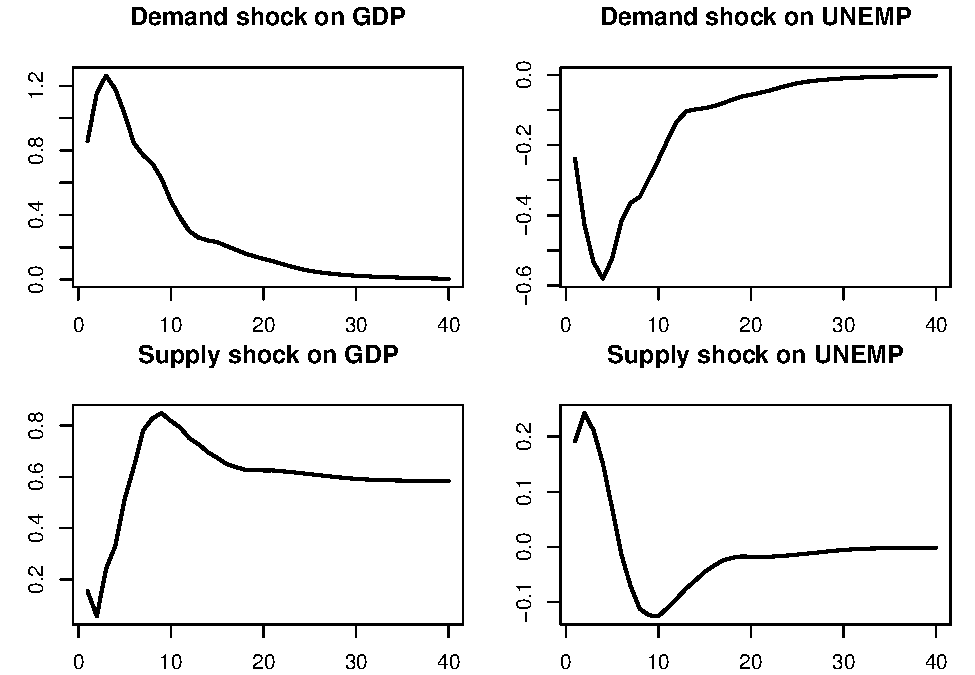
\includegraphics[width=0.95\linewidth]{IdentifStructShocks_files/figure-latex/BQ4-1} \caption{IRF of GDP and unemployment to demand and supply shocks.}\label{fig:BQ4}
\end{figure}

\section{Mixing short- and long-run restrictions}\label{Mixing}

We have seen above that the matrix \(B\) can be identified by imposing \(n(n-1)/2\) restrictions on the short-run or long-run impacts of the shocks. It is also possible to combine short-run and long-run restrictions, provided that their total number still equals \(n(n-1)/2\).

In practice, such hybrid identification schemes often need to be implemented numerically, as closed-form expressions are not always available. To illustrate, consider a three-variable model including the first difference of log GDP, inflation, and a short-term interest rate. We aim to identify three structural shocks. We assume the existence of a supply shock, which is the only shock with a long-run effect on GDP, and two demand shocks (this provides two restrictions). Among the latter, one is a monetary policy shock, identified by imposing that it has no contemporaneous impact on GDP.

The following code chunk implements this identification strategy using Canadian data:

\begin{Shaded}
\begin{Highlighting}[]
\FunctionTok{library}\NormalTok{(vars)   }\CommentTok{\# provides \textquotesingle{}VARselect\textquotesingle{} function}
\FunctionTok{library}\NormalTok{(IdSS)   }\CommentTok{\# dataset is included here}
\CommentTok{\# Make dataset: {-}{-}{-}{-}{-}{-}{-}{-}{-}{-}{-}{-}{-}{-}{-}{-}{-}{-}{-}{-}{-}{-}{-}{-}{-}{-}{-}{-}{-}{-}{-}{-}{-}{-}{-}{-}{-}{-}{-}{-}{-}{-}{-}{-}{-}{-}{-}{-}{-}{-}{-}{-}{-}{-}{-}{-}{-}{-}{-}{-}{-}{-}{-}{-}}
\NormalTok{ctry }\OtherTok{\textless{}{-}} \StringTok{"CAN"} \CommentTok{\# select country in the "international" dataset}
\NormalTok{data }\OtherTok{\textless{}{-}}\NormalTok{ international[,}\FunctionTok{c}\NormalTok{(}\StringTok{"date"}\NormalTok{,}
                         \FunctionTok{paste}\NormalTok{(}\StringTok{"GDP\_"}\NormalTok{,ctry,}\AttributeTok{sep=}\StringTok{""}\NormalTok{),}
                         \FunctionTok{paste}\NormalTok{(}\StringTok{"CPI\_"}\NormalTok{,ctry,}\AttributeTok{sep=}\StringTok{""}\NormalTok{),}
                         \FunctionTok{paste}\NormalTok{(}\StringTok{"STR\_"}\NormalTok{,ctry,}\AttributeTok{sep=}\StringTok{""}\NormalTok{))]}
\NormalTok{data }\OtherTok{\textless{}{-}}\NormalTok{ data[}\FunctionTok{complete.cases}\NormalTok{(data),] }\CommentTok{\# remove missing data}
\NormalTok{TT }\OtherTok{\textless{}{-}} \FunctionTok{dim}\NormalTok{(data)[}\DecValTok{1}\NormalTok{] }\CommentTok{\# sample length}
\NormalTok{data}\SpecialCharTok{$}\NormalTok{dy }\OtherTok{\textless{}{-}}\NormalTok{ data}\SpecialCharTok{$}\NormalTok{GDP\_}
\NormalTok{data}\SpecialCharTok{$}\NormalTok{pi }\OtherTok{\textless{}{-}}\NormalTok{ data}\SpecialCharTok{$}\NormalTok{CPI\_}
\NormalTok{data}\SpecialCharTok{$}\NormalTok{str }\OtherTok{\textless{}{-}}\NormalTok{ data}\SpecialCharTok{$}\NormalTok{STR\_}
\NormalTok{Y }\OtherTok{\textless{}{-}}\NormalTok{ data[}\FunctionTok{c}\NormalTok{(}\StringTok{"dy"}\NormalTok{,}\StringTok{"pi"}\NormalTok{,}\StringTok{"str"}\NormalTok{)]}
\NormalTok{n }\OtherTok{\textless{}{-}} \FunctionTok{dim}\NormalTok{(Y)[}\DecValTok{2}\NormalTok{]}
\CommentTok{\# VAR estimation: {-}{-}{-}{-}{-}{-}{-}{-}{-}{-}{-}{-}{-}{-}{-}{-}{-}{-}{-}{-}{-}{-}{-}{-}{-}{-}{-}{-}{-}{-}{-}{-}{-}{-}{-}{-}{-}{-}{-}{-}{-}{-}{-}{-}{-}{-}{-}{-}{-}{-}{-}{-}{-}{-}{-}{-}{-}{-}{-}{-}{-}{-}}
\NormalTok{p }\OtherTok{\textless{}{-}} \DecValTok{4}
\NormalTok{estVAR }\OtherTok{\textless{}{-}} \FunctionTok{VAR}\NormalTok{(Y, }\AttributeTok{p =}\NormalTok{ p) }\CommentTok{\# estimate the VAR model}
\NormalTok{Phi }\OtherTok{\textless{}{-}} \FunctionTok{Acoef}\NormalTok{(estVAR)}
\NormalTok{eps }\OtherTok{\textless{}{-}} \FunctionTok{residuals}\NormalTok{(estVAR)}
\NormalTok{Omega }\OtherTok{\textless{}{-}} \FunctionTok{var}\NormalTok{(eps) }\CommentTok{\# covariance matrix of OLS residuals}
\CommentTok{\# Indentify B using mixed approach: {-}{-}{-}{-}{-}{-}{-}{-}{-}{-}{-}{-}{-}{-}{-}{-}{-}{-}{-}{-}{-}{-}{-}{-}{-}{-}{-}{-}{-}{-}{-}{-}{-}{-}{-}{-}{-}{-}{-}{-}{-}{-}{-}{-}}
\CommentTok{\# Compute (Id {-} Phi)\^{}\{{-}1\}:}
\NormalTok{PHI }\OtherTok{\textless{}{-}} \FunctionTok{make.PHI}\NormalTok{(Phi)}
\NormalTok{sum.PHI.k }\OtherTok{\textless{}{-}} \FunctionTok{solve}\NormalTok{(}\FunctionTok{diag}\NormalTok{(}\FunctionTok{dim}\NormalTok{(PHI)[}\DecValTok{1}\NormalTok{]) }\SpecialCharTok{{-}}\NormalTok{ PHI)[}\DecValTok{1}\SpecialCharTok{:}\NormalTok{n,}\DecValTok{1}\SpecialCharTok{:}\NormalTok{n]}
\CommentTok{\# Define loss function:}
\NormalTok{loss }\OtherTok{\textless{}{-}} \ControlFlowTok{function}\NormalTok{(param)\{}
\NormalTok{  B }\OtherTok{\textless{}{-}} \FunctionTok{matrix}\NormalTok{(param,n,n)}
\NormalTok{  X }\OtherTok{\textless{}{-}}\NormalTok{ Omega }\SpecialCharTok{{-}}\NormalTok{ B }\SpecialCharTok{\%*\%} \FunctionTok{t}\NormalTok{(B)}
\NormalTok{  Theta }\OtherTok{\textless{}{-}}\NormalTok{ sum.PHI.k[}\DecValTok{1}\SpecialCharTok{:}\NormalTok{n,}\DecValTok{1}\SpecialCharTok{:}\NormalTok{n] }\SpecialCharTok{\%*\%}\NormalTok{ B}
\NormalTok{  loss }\OtherTok{\textless{}{-}} \DecValTok{100000} \SpecialCharTok{*}\NormalTok{ ( }\FunctionTok{sum}\NormalTok{(X}\SpecialCharTok{\^{}}\DecValTok{2}\NormalTok{) }\SpecialCharTok{+}\NormalTok{ Theta[}\DecValTok{1}\NormalTok{,}\DecValTok{2}\NormalTok{]}\SpecialCharTok{\^{}}\DecValTok{2} \SpecialCharTok{+}\NormalTok{ Theta[}\DecValTok{1}\NormalTok{,}\DecValTok{3}\NormalTok{]}\SpecialCharTok{\^{}}\DecValTok{2} \SpecialCharTok{+}\NormalTok{ B[}\DecValTok{1}\NormalTok{,}\DecValTok{3}\NormalTok{]}\SpecialCharTok{\^{}}\DecValTok{2}\NormalTok{)}
  \FunctionTok{return}\NormalTok{(loss)}
\NormalTok{\}}
\NormalTok{res.opt }\OtherTok{\textless{}{-}} \FunctionTok{optim}\NormalTok{(}\FunctionTok{c}\NormalTok{(}\FunctionTok{diag}\NormalTok{(n)),loss,}\AttributeTok{method=}\StringTok{"BFGS"}\NormalTok{,}\AttributeTok{hessian=}\ConstantTok{FALSE}\NormalTok{)}
\NormalTok{B }\OtherTok{\textless{}{-}} \FunctionTok{matrix}\NormalTok{(res.opt}\SpecialCharTok{$}\NormalTok{par,n,n)}
\CommentTok{\# Make IRFs: {-}{-}{-}{-}{-}{-}{-}{-}{-}{-}{-}{-}{-}{-}{-}{-}{-}{-}{-}{-}{-}{-}{-}{-}{-}{-}{-}{-}{-}{-}{-}{-}{-}{-}{-}{-}{-}{-}{-}{-}{-}{-}{-}{-}{-}{-}{-}{-}{-}{-}{-}{-}{-}{-}{-}{-}{-}{-}{-}{-}{-}{-}{-}{-}{-}{-}{-}}
\NormalTok{n }\OtherTok{\textless{}{-}} \FunctionTok{dim}\NormalTok{(Y)[}\DecValTok{2}\NormalTok{] }\CommentTok{\# number of endogenous variables}
\FunctionTok{par}\NormalTok{(}\AttributeTok{mfrow =} \FunctionTok{c}\NormalTok{(n, n))}
\FunctionTok{par}\NormalTok{(}\AttributeTok{plt =} \FunctionTok{c}\NormalTok{(.}\DecValTok{3}\NormalTok{, .}\DecValTok{95}\NormalTok{, .}\DecValTok{2}\NormalTok{, .}\DecValTok{75}\NormalTok{))}
\NormalTok{Model }\OtherTok{\textless{}{-}} \FunctionTok{list}\NormalTok{(}\AttributeTok{c =}\NormalTok{ c, }\AttributeTok{Phi =}\NormalTok{ Phi, }\AttributeTok{B =}\NormalTok{ B)}
\NormalTok{names.var }\OtherTok{\textless{}{-}} \FunctionTok{c}\NormalTok{(}\StringTok{"log(GDP)"}\NormalTok{, }\StringTok{"Inflation"}\NormalTok{, }\StringTok{"Interest rate"}\NormalTok{)}
\ControlFlowTok{for}\NormalTok{ (variable }\ControlFlowTok{in} \DecValTok{1}\SpecialCharTok{:}\NormalTok{n) \{}
  \ControlFlowTok{for}\NormalTok{ (shock }\ControlFlowTok{in} \DecValTok{1}\SpecialCharTok{:}\NormalTok{n) \{}
\NormalTok{    eta0 }\OtherTok{\textless{}{-}} \FunctionTok{rep}\NormalTok{(}\DecValTok{0}\NormalTok{, n)}
\NormalTok{    eta0[shock] }\OtherTok{\textless{}{-}} \DecValTok{1}
\NormalTok{    res.sim }\OtherTok{\textless{}{-}} \FunctionTok{simul.VAR}\NormalTok{(}\AttributeTok{c =} \ConstantTok{NaN}\NormalTok{, Phi, B, }\AttributeTok{nb.sim =} \DecValTok{60}\NormalTok{, }\AttributeTok{indic.IRF =} \DecValTok{1}\NormalTok{,}
                         \AttributeTok{u.shock =}\NormalTok{ eta0)}
    \ControlFlowTok{if}\NormalTok{(variable}\SpecialCharTok{==}\DecValTok{1}\NormalTok{)\{}\CommentTok{\# For GDP, show cumulated growth rates (i.e., log(GDP)):}
\NormalTok{      irf }\OtherTok{\textless{}{-}} \FunctionTok{cumsum}\NormalTok{(res.sim[, variable])}
\NormalTok{    \}}\ControlFlowTok{else}\NormalTok{\{}
\NormalTok{      irf }\OtherTok{\textless{}{-}}\NormalTok{ res.sim[, variable]}
\NormalTok{    \}}
    \FunctionTok{plot}\NormalTok{(irf, }\AttributeTok{type =} \StringTok{"l"}\NormalTok{, }\AttributeTok{lwd =} \DecValTok{2}\NormalTok{, }\AttributeTok{las =} \DecValTok{1}\NormalTok{,}
         \AttributeTok{xlab =} \StringTok{""}\NormalTok{, }\AttributeTok{ylab =} \FunctionTok{ifelse}\NormalTok{(shock}\SpecialCharTok{==}\DecValTok{1}\NormalTok{,}
                                  \FunctionTok{paste}\NormalTok{(}\StringTok{"Resp. of "}\NormalTok{,}
\NormalTok{                                              names.var[variable],}\StringTok{"..."}\NormalTok{,}\AttributeTok{sep=}\StringTok{""}\NormalTok{),}\StringTok{""}\NormalTok{),}
         \AttributeTok{main =} \FunctionTok{ifelse}\NormalTok{(variable}\SpecialCharTok{==}\DecValTok{1}\NormalTok{,}\FunctionTok{paste}\NormalTok{(}\StringTok{"... to shock η"}\NormalTok{, shock, }\AttributeTok{sep =} \StringTok{""}\NormalTok{),}\StringTok{""}\NormalTok{))\}\}}
\end{Highlighting}
\end{Shaded}

\pandocbounded{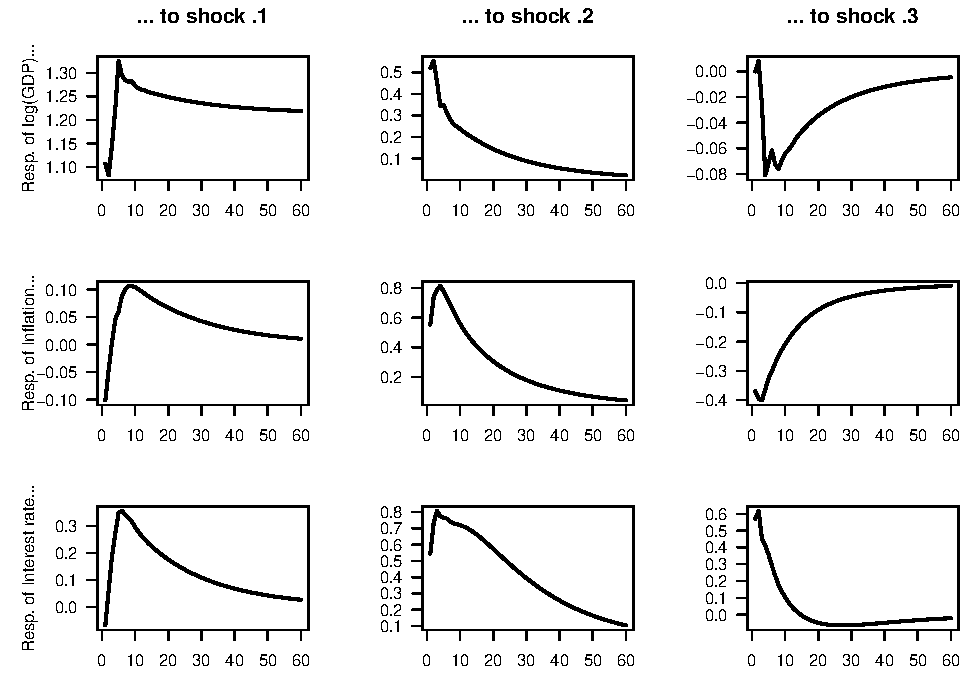
\includegraphics[keepaspectratio]{IdentifStructShocks_files/figure-latex/unnamed-chunk-11-1.pdf}}

\chapter{Inference}\label{Inference}

Consider the following SVAR model:
\[y_t = \Phi_1 y_{t-1} + \dots + \Phi_p y_{t-p} + \varepsilon_t\]
where \(\varepsilon_t\) is a white noise sequence. This vector rewrites \(\varepsilon_t=B\eta_t\) where \(\mathbb{V}ar(\eta_t)=I\), which implies \(\Omega_\varepsilon=BB'\).

The corresponding infinite MA representation (Eq. \eqref{eq:InfMA}, or Wold representation, is:
\[
y_t = \sum_{h=0}^\infty\Psi_h \eta_{t-h},
\]
where \(\Psi_0=B\) and for \(h=1,2,\dots\):
\[
\Psi_h = \sum_{j=1}^h\Psi_{h-j}\Phi_j,
\]
with \(\Phi_j=0\) for \(j>p\) (see Prop. \ref{prp:computPsi} for this recursive computation of the \(\Psi_j\)'s).

Inference on the VAR coefficients \(\{\Phi_j\}_{j=1,...,p}\) is straightforward (standard OLS inference). But inference is more complicated regarding IRFs. Indeed, as shown by the previous equation, the (infinite) MA coefficients \(\{\Psi_j\}_{j=1,...}\) are non-linear functions of the \(\{\Phi_j\}_{j=1,...,p}\) and of \(\Omega_\varepsilon\). An other issue pertain to small sample bias: typically, for persistent processes, auto-regressive parameters are known to be downward biased.

The main inference methods are the following:

\begin{itemize}
\tightlist
\item
  Monte Carlo method (\citet{Hamilton_1994}) (Section \ref{MonteCarlo});
\item
  Asymptotic normal approximation (\citet{Lutkepohl_1990}), or Delta method (Section \ref{Delta});
\item
  Bootstrap method (\citet{Kilian_1998}) (Sections \ref{Bootstrap1} and \ref{BootstrapAfter}).
\end{itemize}

\section{Monte Carlo method}\label{MonteCarlo}

We use Monte Carlo when we need to approximate the distribution of a variable whose distribution is unknown (here: the \(\Psi_j\)'s) but which is a function of another variable whose distribution is known (here, the \(\Phi_j\)'s).

For instance, suppose we know the distribution of a random variable \(X\), which takes values in \(\mathbb{R}\), with density function \(p\). Assume we want to compute the mean of \(\varphi(X)\). We have:
\[
\mathbb{E}(\varphi(X))=\int_{-\infty}^{+\infty}\varphi(x)p(x)dx
\]
Suppose that the above integral does not have a simple expression. We cannot compute \(\mathbb{E}(\varphi(X))\) but, by virtue of the law of large numbers, we can approximate it as follows:
\[
\mathbb{E}(\varphi(X))\approx\frac{1}{N}\sum_{i=1}^N\varphi(X^{(i)}),
\]
where \(\{X^{(i)}\}_{i=1,...,N}\) are \(N\) independent draws of \(X\). More generally, the distribution of \(\varphi(X)\) can be approximated by the empirical distribution of the \(\varphi(X^{(i)})\)'s. Typically, if 10'000 values of \(\varphi(X^{(i)})\) are drawn, the \(5^{th}\) percentile of the p.d.f. of \(\varphi(X)\) can be approximated by the \(500^{th}\) value of the 10'000 draws of \(\varphi(X^{(i)})\) (after arranging these values in ascending order).

As regards the computation of confidence intervals around IRFs, one has to think of \(\{\widehat{\Phi}_j\}_{j=1,...,p}\), and of \(\widehat{\Omega}\) as \(X\) and \(\{\widehat{\Psi}_j\}_{j=1,...}\) as \(\varphi(X)\). (Proposition \ref{prp:OLSVAR2} provides us with the asymptotic distribution of the ``\(X\).'')

To summarize, here are the steps one can implement to derive confidence intervals for the IRFs using the Monte-Carlo approach: For each iteration \(k\),

\begin{enumerate}
\def\labelenumi{\arabic{enumi}.}
\tightlist
\item
  Draw \(\{\widehat{\Phi}_j^{(k)}\}_{j=1,...,p}\) and \(\widehat{\Omega}^{(k)}\) from their asymptotic distribution (using Proposition \ref{prp:OLSVAR2}).
\item
  Compute the matrix \(B^{(k)}\) so that \(\widehat{\Omega}^{(k)}=B^{(k)}B^{(k)'}\), according to your identification strategy.
\item
  Compute the associated IRFs \(\{\widehat{\Psi}_j\}^{(k)}\).
\end{enumerate}

Perform \(N\) replications and report the median impulse response (and its confidence intervals).

The following code implements the Monte Carlo method.

\begin{Shaded}
\begin{Highlighting}[]
\FunctionTok{library}\NormalTok{(IdSS);}\FunctionTok{library}\NormalTok{(vars);}\FunctionTok{library}\NormalTok{(Matrix)}
\FunctionTok{data}\NormalTok{(}\StringTok{"USmonthly"}\NormalTok{)}
\NormalTok{First.date }\OtherTok{\textless{}{-}} \StringTok{"1965{-}01{-}01"}
\NormalTok{Last.date }\OtherTok{\textless{}{-}} \StringTok{"1995{-}06{-}01"}
\NormalTok{indic.first }\OtherTok{\textless{}{-}} \FunctionTok{which}\NormalTok{(USmonthly}\SpecialCharTok{$}\NormalTok{DATES}\SpecialCharTok{==}\NormalTok{First.date)}
\NormalTok{indic.last  }\OtherTok{\textless{}{-}} \FunctionTok{which}\NormalTok{(USmonthly}\SpecialCharTok{$}\NormalTok{DATES}\SpecialCharTok{==}\NormalTok{Last.date)}
\NormalTok{USmonthly   }\OtherTok{\textless{}{-}}\NormalTok{ USmonthly[indic.first}\SpecialCharTok{:}\NormalTok{indic.last,]}
\NormalTok{considered.variables}\OtherTok{\textless{}{-}}\FunctionTok{c}\NormalTok{(}\StringTok{"LIP"}\NormalTok{,}\StringTok{"UNEMP"}\NormalTok{,}\StringTok{"LCPI"}\NormalTok{,}\StringTok{"LPCOM"}\NormalTok{,}\StringTok{"FFR"}\NormalTok{,}\StringTok{"NBR"}\NormalTok{,}\StringTok{"TTR"}\NormalTok{,}\StringTok{"M1"}\NormalTok{)}
\NormalTok{y }\OtherTok{\textless{}{-}} \FunctionTok{as.matrix}\NormalTok{(USmonthly[considered.variables])}
\CommentTok{\# ===================================}
\CommentTok{\# CEE with Monte Carlo}
\CommentTok{\# ===================================}
\NormalTok{res.svar.ordering }\OtherTok{\textless{}{-}}
  \FunctionTok{svar.ordering.2}\NormalTok{(y,}\AttributeTok{p=}\DecValTok{3}\NormalTok{,}
                  \AttributeTok{posit.of.shock =} \DecValTok{5}\NormalTok{,}
                  \AttributeTok{nb.periods.IRF =} \DecValTok{20}\NormalTok{,}
                  \AttributeTok{inference =} \DecValTok{3}\NormalTok{,}\CommentTok{\# 0 {-}\textgreater{} no inference, 1 {-}\textgreater{} parametric bootst.,}
                  \CommentTok{\# 2 \textless{}{-} non{-}parametric bootstrap, 3 \textless{}{-} Monte Carlo,}
                  \CommentTok{\# 4 \textless{}{-} bootstrap{-}after{-}bootstrap}
                  \AttributeTok{nb.draws =} \DecValTok{200}\NormalTok{,}
                  \AttributeTok{confidence.interval =} \FloatTok{0.90}\NormalTok{, }\CommentTok{\# expressed in pp.}
                  \AttributeTok{indic.plot =} \DecValTok{1} \CommentTok{\# Plots are displayed if = 1.}
\NormalTok{  )}
\end{Highlighting}
\end{Shaded}

\begin{figure}
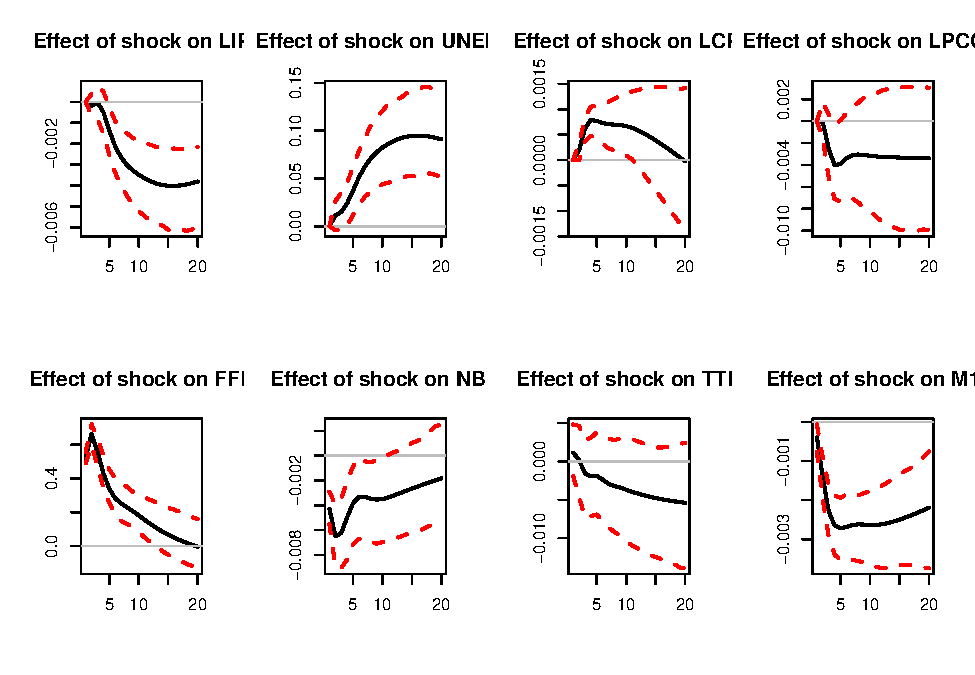
\includegraphics[width=0.95\linewidth]{IdentifStructShocks_files/figure-latex/inference1-1} \caption{IRF associated with a monetary policy shock; Monte Carlo method.}\label{fig:inference1}
\end{figure}

\begin{Shaded}
\begin{Highlighting}[]
\NormalTok{IRFs.ordering }\OtherTok{\textless{}{-}}\NormalTok{ res.svar.ordering}\SpecialCharTok{$}\NormalTok{IRFs}
\NormalTok{median.IRFs.ordering }\OtherTok{\textless{}{-}}\NormalTok{ res.svar.ordering}\SpecialCharTok{$}\NormalTok{all.CI.median}
\NormalTok{simulated.IRFs.ordering }\OtherTok{\textless{}{-}}\NormalTok{ res.svar.ordering}\SpecialCharTok{$}\NormalTok{simulated.IRFs}
\end{Highlighting}
\end{Shaded}

Below we plot the estimated IRFs to a mom\^{}netary policy shock, together with a sample of 50 IRFs simulated with the Monte Carlo method, and the median of all simulated IRFs.

\begin{Shaded}
\begin{Highlighting}[]
\FunctionTok{par}\NormalTok{(}\AttributeTok{mfrow=}\FunctionTok{c}\NormalTok{(}\DecValTok{1}\NormalTok{,}\DecValTok{1}\NormalTok{))}
\FunctionTok{plot}\NormalTok{(IRFs.ordering[,}\DecValTok{5}\NormalTok{],}\AttributeTok{type=}\StringTok{"l"}\NormalTok{)}
\ControlFlowTok{for}\NormalTok{(i }\ControlFlowTok{in} \DecValTok{1}\SpecialCharTok{:}\DecValTok{50}\NormalTok{)\{}
  \FunctionTok{lines}\NormalTok{(simulated.IRFs.ordering[,}\DecValTok{5}\NormalTok{,i],}\AttributeTok{col=}\StringTok{"red"}\NormalTok{,}\AttributeTok{type=}\StringTok{"l"}\NormalTok{)}
\NormalTok{\}}
\FunctionTok{lines}\NormalTok{(IRFs.ordering[,}\DecValTok{5}\NormalTok{],}\AttributeTok{col=}\StringTok{"black"}\NormalTok{,}\AttributeTok{type=}\StringTok{"l"}\NormalTok{)}
\FunctionTok{lines}\NormalTok{(median.IRFs.ordering[,}\DecValTok{5}\NormalTok{],}\AttributeTok{col=}\StringTok{"blue"}\NormalTok{,}\AttributeTok{type=}\StringTok{"l"}\NormalTok{)}
\end{Highlighting}
\end{Shaded}

\begin{figure}
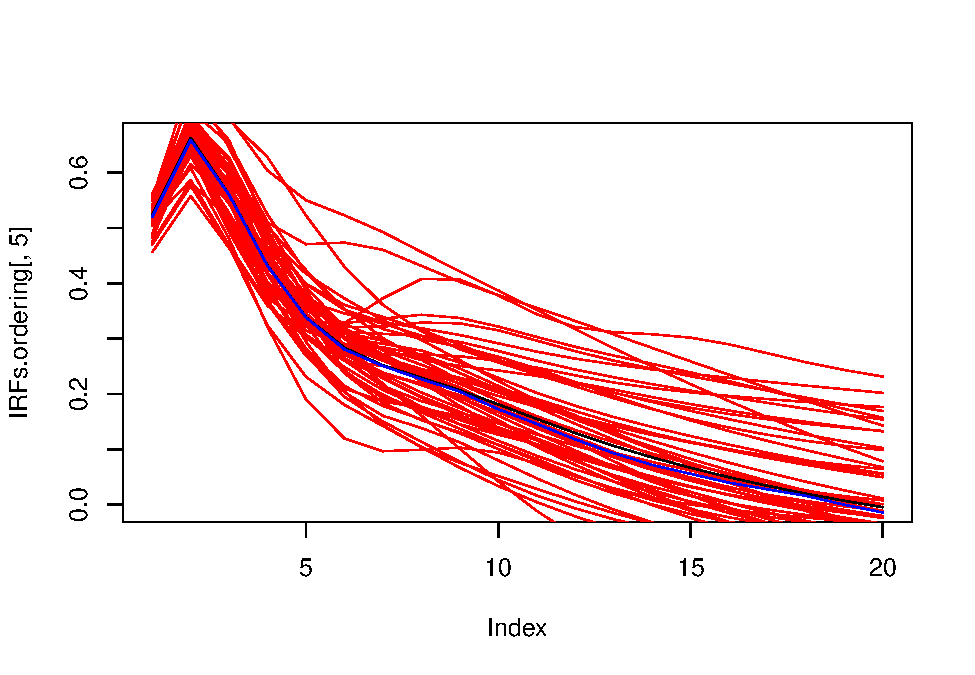
\includegraphics[width=0.95\linewidth]{IdentifStructShocks_files/figure-latex/inference1bis-1} \caption{Estimated IRF associated with a monetary policy shock (black line) with simulated IRFs (red lines) and median IRF (blue line); Monte Carlo method.}\label{fig:inference1bis}
\end{figure}

\section{Delta method}\label{Delta}

Suppose \(\beta\) is a vector of parameters and \(\hat\beta\) is an estimator such that
\[
\sqrt{T}\,(\hat\beta-\beta)\overset{d}{\longrightarrow}\mathcal{N}(0,\Sigma_\beta),
\]
where \(\overset{d}{\longrightarrow}\) denotes convergence in distribution, \(\mathcal{N}(0,\Sigma_\beta)\) denotes a multivariate normal distribution with mean vector \(0\) and covariance matrix \(\Sigma_\beta\), and \(T\) is the sample size.

Let \(\varphi(\beta) = (\varphi_1(\beta),\dots,\varphi_m(\beta))'\) be a continuously differentiable function with values in \(\mathbb{R}^m\), and assume that \(\partial \varphi_i/\partial \beta'\) is nonzero at \(\beta\) for \(i = 1,\dots,m\). Then, if \(\varphi\) is not too nonlinear in a neighborhood of \(\beta\), we approximately have
\[
\sqrt{T}\,(\varphi(\hat\beta)-\varphi(\beta))
\overset{d}{\approx}
\mathcal{N}\!\left(
0,\;
\frac{\partial \varphi}{\partial \beta'}
\Sigma_\beta
\frac{\partial \varphi'}{\partial \beta}
\right),
\]
where \(\frac{\partial \varphi}{\partial \beta'}\) denotes the Jacobian of \(\varphi\) with respect to \(\beta'\).

Using this property, \citet{Lutkepohl_1990} provides the asymptotic distributions of the \(\Psi_j\)'s.

A limit of the last two approaches (Monte Carlo and the Delta method) is that they rely on asymptotic results and the normality assumption. Boostrapping approaches are more robust in small-sample and non-normal situations.

\section{Bootstrap}\label{Bootstrap1}

IRFs' confidence intervals are intervals where 90\% (or 95\%, 75\%, \ldots) of the IRFs would lie, if we were to repeat the estimation a large number of times in similar conditions (\(T\) observations). We obviously cannot do this, because we have only one sample: \(\{y_t\}_{t=1,..,T}\). But we can try to \emph{construct} such samples.

Bootstrapping consists in:

\begin{itemize}
\tightlist
\item
  re-sampling \(N\) times, i.e., constructing \(N\) samples of \(T\) observations, using the estimated
  VAR coefficients and
\end{itemize}

\begin{enumerate}
\def\labelenumi{\alph{enumi}.}
\tightlist
\item
  a sample of residuals from the distribution \(\mathcal{N}(0,BB')\) (\textbf{parametric approach}), or
\item
  a sample of residuals drawn randomly from the set of the actual estimated residuals \(\{\hat\varepsilon_t\}_{t=1,..,T}\). (\textbf{non-parametric approach}).
\end{enumerate}

\begin{itemize}
\tightlist
\item
  re-estimating the SVAR \(N\) times.
\end{itemize}

Here is the algorithm for the non-parametric approach:

\begin{enumerate}
\def\labelenumi{\arabic{enumi}.}
\tightlist
\item
  Construct a sample
  \[
  y_t^{(k)}=\widehat{\Phi}_1 y_{t-1}^{(k)} + \dots + \widehat{\Phi}_p y_{t-p}^{(k)} + \hat\varepsilon_t^{(k)},
  \]
  with \(\hat\varepsilon_{t}^{(k)}=\hat\varepsilon_{s_t^{(k)}}\), where \(\{s_1^{(k)},..,s_T^{(k)}\}\) is a random set from \(\{1,..,T\}^T\). (Note: in the parametric approach, we would draw \(\hat\varepsilon_{t}^{(k)}\) from the \(\mathcal{N}(0,BB')\) distribution)
\item
  Re-estimate the SVAR and compute the IRFs \(\{\widehat{\Psi}_j\}^{(k)}\).
\end{enumerate}

Perform \(N\) replications and report the median impulse response (and its confidence intervals).

The following code implements the bootstrap method.

\begin{Shaded}
\begin{Highlighting}[]
\FunctionTok{library}\NormalTok{(IdSS);}\FunctionTok{library}\NormalTok{(vars);}\FunctionTok{library}\NormalTok{(Matrix)}
\FunctionTok{data}\NormalTok{(}\StringTok{"USmonthly"}\NormalTok{)}
\NormalTok{First.date }\OtherTok{\textless{}{-}} \StringTok{"1965{-}01{-}01"}
\NormalTok{Last.date }\OtherTok{\textless{}{-}} \StringTok{"1995{-}06{-}01"}
\NormalTok{indic.first }\OtherTok{\textless{}{-}} \FunctionTok{which}\NormalTok{(USmonthly}\SpecialCharTok{$}\NormalTok{DATES}\SpecialCharTok{==}\NormalTok{First.date)}
\NormalTok{indic.last  }\OtherTok{\textless{}{-}} \FunctionTok{which}\NormalTok{(USmonthly}\SpecialCharTok{$}\NormalTok{DATES}\SpecialCharTok{==}\NormalTok{Last.date)}
\NormalTok{USmonthly   }\OtherTok{\textless{}{-}}\NormalTok{ USmonthly[indic.first}\SpecialCharTok{:}\NormalTok{indic.last,]}
\NormalTok{considered.variables}\OtherTok{\textless{}{-}}\FunctionTok{c}\NormalTok{(}\StringTok{"LIP"}\NormalTok{,}\StringTok{"UNEMP"}\NormalTok{,}\StringTok{"LCPI"}\NormalTok{,}\StringTok{"LPCOM"}\NormalTok{,}\StringTok{"FFR"}\NormalTok{,}\StringTok{"NBR"}\NormalTok{,}\StringTok{"TTR"}\NormalTok{,}\StringTok{"M1"}\NormalTok{)}
\NormalTok{y }\OtherTok{\textless{}{-}} \FunctionTok{as.matrix}\NormalTok{(USmonthly[considered.variables])}
\CommentTok{\# ===================================}
\CommentTok{\# CEE with bootstrap}
\CommentTok{\# ===================================}
\NormalTok{res.svar.ordering }\OtherTok{\textless{}{-}}
  \FunctionTok{svar.ordering.2}\NormalTok{(y,}\AttributeTok{p=}\DecValTok{3}\NormalTok{,}
                  \AttributeTok{posit.of.shock =} \DecValTok{5}\NormalTok{,}
                  \AttributeTok{nb.periods.IRF =} \DecValTok{20}\NormalTok{,}
                  \AttributeTok{inference =} \DecValTok{2}\NormalTok{,}\CommentTok{\# 0 {-}\textgreater{} no inference, 1 {-}\textgreater{} parametric bootstr.,}
                  \CommentTok{\# 2 \textless{}{-} non{-}parametric bootstrap, 3 \textless{}{-} monte carlo,}
                  \CommentTok{\# 4 \textless{}{-} bootstrap{-}after{-}bootstrap}
                  \AttributeTok{nb.draws =} \DecValTok{200}\NormalTok{,}
                  \AttributeTok{confidence.interval =} \FloatTok{0.90}\NormalTok{, }\CommentTok{\# expressed in pp.}
                  \AttributeTok{indic.plot =} \DecValTok{1} \CommentTok{\# Plots are displayed if = 1.}
\NormalTok{  )}
\end{Highlighting}
\end{Shaded}

\begin{figure}
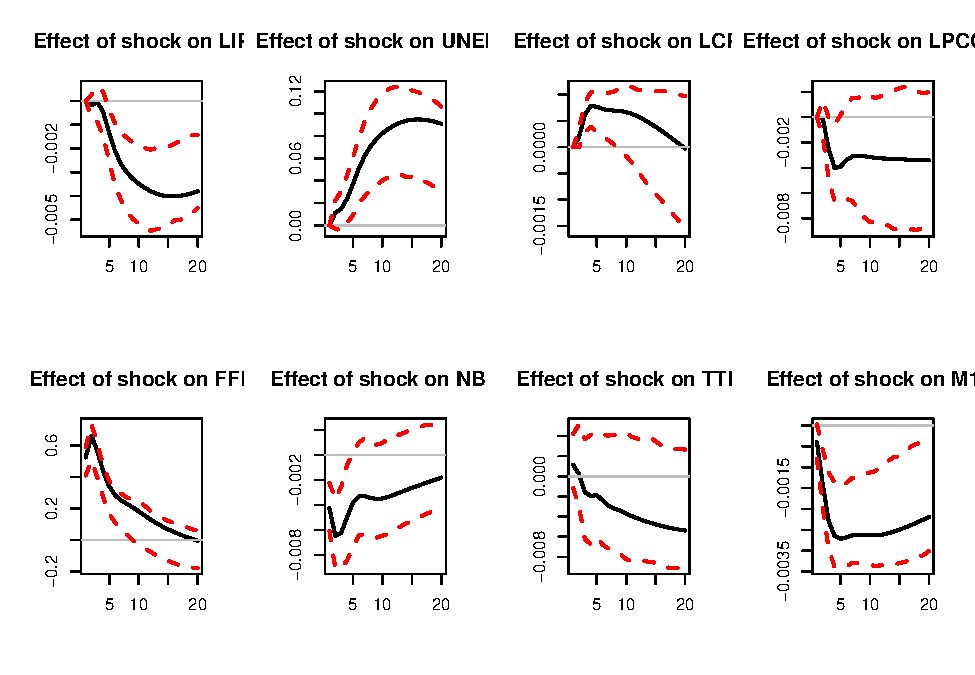
\includegraphics[width=0.95\linewidth]{IdentifStructShocks_files/figure-latex/inference2-1} \caption{IRF associated with a monetary policy shock; bootstrap method.}\label{fig:inference2}
\end{figure}

\begin{Shaded}
\begin{Highlighting}[]
\NormalTok{IRFs.ordering.bootstrap }\OtherTok{\textless{}{-}}\NormalTok{ res.svar.ordering}\SpecialCharTok{$}\NormalTok{IRFs}
\NormalTok{median.IRFs.ordering.bootstrap }\OtherTok{\textless{}{-}}\NormalTok{ res.svar.ordering}\SpecialCharTok{$}\NormalTok{all.CI.median}
\NormalTok{simulated.IRFs.ordering.bootstrap }\OtherTok{\textless{}{-}}\NormalTok{ res.svar.ordering}\SpecialCharTok{$}\NormalTok{simulated.IRFs}
\end{Highlighting}
\end{Shaded}

\section{Bootstrap-after-bootstrap}\label{BootstrapAfter}

The previous simple bootstrapping procedure deals with non-normality and small sample distribution, since we use the actual residuals. However, it does not deal with the \emph{small sample bias}, stemming, in particular, from small-sample bias associated with OLS coefficient estimates \(\{\widehat{\Phi}_j\}_{j=1,..,p}\).

The code below illustrates the small sample bias.

\begin{Shaded}
\begin{Highlighting}[]
\CommentTok{\# Distribution of coefficients stemming from non{-}parametric bootstrap}
\NormalTok{n }\OtherTok{\textless{}{-}} \FunctionTok{length}\NormalTok{(considered.variables)}
\NormalTok{h }\OtherTok{\textless{}{-}} \DecValTok{5}
\FunctionTok{par}\NormalTok{(}\AttributeTok{mfrow=}\FunctionTok{c}\NormalTok{(}\DecValTok{2}\NormalTok{,}\FunctionTok{ifelse}\NormalTok{(}\FunctionTok{round}\NormalTok{(n}\SpecialCharTok{/}\DecValTok{2}\NormalTok{)}\SpecialCharTok{==}\NormalTok{n}\SpecialCharTok{/}\DecValTok{2}\NormalTok{,n}\SpecialCharTok{/}\DecValTok{2}\NormalTok{,(n}\SpecialCharTok{+}\DecValTok{1}\NormalTok{)}\SpecialCharTok{/}\DecValTok{2}\NormalTok{)))}
\ControlFlowTok{for}\NormalTok{ (i }\ControlFlowTok{in} \DecValTok{1}\SpecialCharTok{:}\NormalTok{n)\{}
  \FunctionTok{hist}\NormalTok{(simulated.IRFs.ordering.bootstrap[h,i,],}\AttributeTok{xlab=}\StringTok{""}\NormalTok{,}\AttributeTok{ylab=}\StringTok{""}\NormalTok{,}
       \AttributeTok{main=}\FunctionTok{paste}\NormalTok{(}\StringTok{"Effect at h = "}\NormalTok{,h,}\StringTok{" on "}\NormalTok{,}
\NormalTok{                  considered.variables[i],}\AttributeTok{sep=}\StringTok{""}\NormalTok{),}\AttributeTok{cex.main=}\NormalTok{.}\DecValTok{9}\NormalTok{)}
  \FunctionTok{lines}\NormalTok{(}\FunctionTok{array}\NormalTok{(}\FunctionTok{c}\NormalTok{(IRFs.ordering.bootstrap[h,i],}
\NormalTok{                IRFs.ordering.bootstrap[h,i],}\DecValTok{0}\NormalTok{,}\DecValTok{100}\NormalTok{),}\FunctionTok{c}\NormalTok{(}\DecValTok{2}\NormalTok{,}\DecValTok{2}\NormalTok{)),}\AttributeTok{col=}\StringTok{"red"}\NormalTok{)}
  \FunctionTok{lines}\NormalTok{(}\FunctionTok{array}\NormalTok{(}\FunctionTok{c}\NormalTok{(median.IRFs.ordering.bootstrap[h,i],}
\NormalTok{                median.IRFs.ordering.bootstrap[h,i],}\DecValTok{0}\NormalTok{,}\DecValTok{100}\NormalTok{),}\FunctionTok{c}\NormalTok{(}\DecValTok{2}\NormalTok{,}\DecValTok{2}\NormalTok{)),}\AttributeTok{col=}\StringTok{"blue"}\NormalTok{)}
  \FunctionTok{text}\NormalTok{(IRFs.ordering.bootstrap[h,i],}\DecValTok{25}\NormalTok{,}\AttributeTok{label=}\StringTok{"Estimated coef."}\NormalTok{,}\AttributeTok{col=}\StringTok{"red"}\NormalTok{)}
\NormalTok{\}}
\end{Highlighting}
\end{Shaded}

\begin{figure}
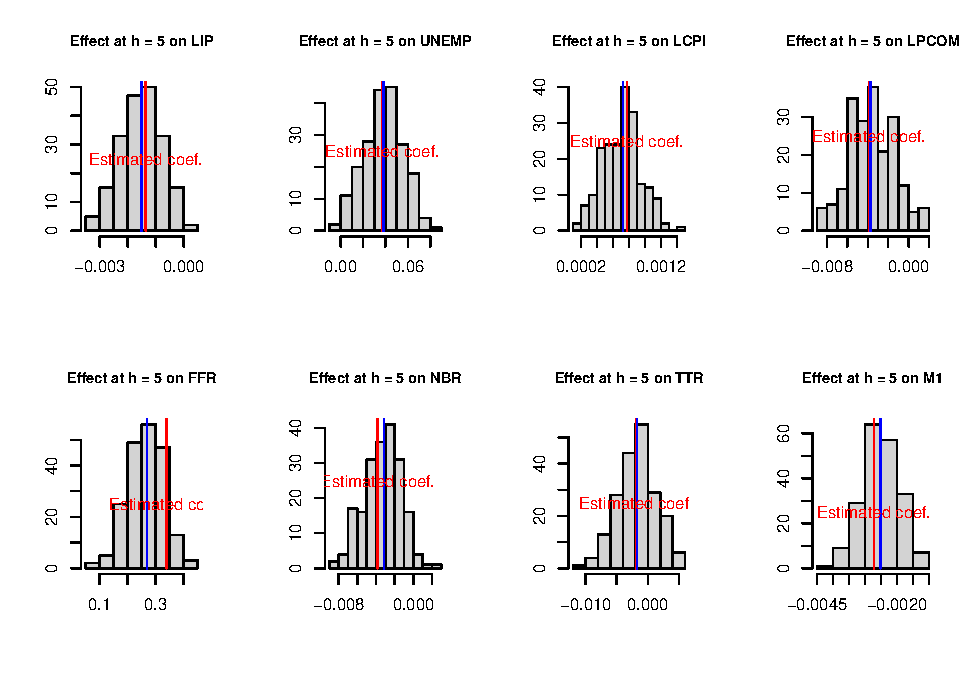
\includegraphics[width=0.95\linewidth]{IdentifStructShocks_files/figure-latex/inference3-1} \caption{Estimated and bootstrapped coefficients.}\label{fig:inference3}
\end{figure}

The distribution of the bootstrapped coefficients is not centered around the estimated coefficients.

In the following code, we perform the VAR estimation and bootstrap inference after generating artificial data. We can then compare the IRFs and confidence intervals to the ``true'\,' parameters used to generate the data.

\begin{Shaded}
\begin{Highlighting}[]
\CommentTok{\# Simulate a small sample}
\NormalTok{est.VAR }\OtherTok{\textless{}{-}} \FunctionTok{VAR}\NormalTok{(y,}\AttributeTok{p=}\DecValTok{3}\NormalTok{)}
\NormalTok{Phi     }\OtherTok{\textless{}{-}} \FunctionTok{Acoef}\NormalTok{(est.VAR)}
\NormalTok{cst     }\OtherTok{\textless{}{-}} \FunctionTok{Bcoef}\NormalTok{(est.VAR)[,}\DecValTok{3}\SpecialCharTok{*}\NormalTok{n}\SpecialCharTok{+}\DecValTok{1}\NormalTok{]}
\NormalTok{resids  }\OtherTok{\textless{}{-}} \FunctionTok{residuals}\NormalTok{(est.VAR)}
\NormalTok{Omega   }\OtherTok{\textless{}{-}} \FunctionTok{var}\NormalTok{(resids)}
\NormalTok{B.hat   }\OtherTok{\textless{}{-}} \FunctionTok{t}\NormalTok{(}\FunctionTok{chol}\NormalTok{(Omega))}
\NormalTok{y0.star }\OtherTok{\textless{}{-}} \ConstantTok{NULL}
\ControlFlowTok{for}\NormalTok{(k }\ControlFlowTok{in} \DecValTok{3}\SpecialCharTok{:}\DecValTok{1}\NormalTok{)\{}
\NormalTok{  y0.star }\OtherTok{\textless{}{-}} \FunctionTok{c}\NormalTok{(y0.star,y[k,])}
\NormalTok{\}}
\NormalTok{small.sample }\OtherTok{\textless{}{-}} \FunctionTok{simul.VAR}\NormalTok{(}\AttributeTok{c=}\FunctionTok{rep}\NormalTok{(}\DecValTok{0}\NormalTok{,}\FunctionTok{dim}\NormalTok{(y)[}\DecValTok{2}\NormalTok{]),}
\NormalTok{                          Phi,}
\NormalTok{                          B.hat,}
                          \AttributeTok{nb.sim =} \DecValTok{100}\NormalTok{,}
\NormalTok{                          y0.star,}
                          \AttributeTok{indic.IRF =} \DecValTok{0}\NormalTok{)}
\FunctionTok{colnames}\NormalTok{(small.sample)  }\OtherTok{\textless{}{-}}\NormalTok{ considered.variables}
\CommentTok{\# Estimate the VAR with the small sample}
\NormalTok{res.svar.small.sample }\OtherTok{\textless{}{-}}
  \FunctionTok{svar.ordering.2}\NormalTok{(small.sample,}\AttributeTok{p=}\DecValTok{3}\NormalTok{,}
                  \AttributeTok{posit.of.shock =} \DecValTok{5}\NormalTok{,}
                  \AttributeTok{nb.periods.IRF =} \DecValTok{20}\NormalTok{,}
                  \AttributeTok{inference =} \DecValTok{2}\NormalTok{,}\CommentTok{\# 0 {-}\textgreater{} no inference, 1 {-}\textgreater{} parametric bootstr.,}
                  \CommentTok{\# 2 \textless{}{-} non{-}parametric bootstrap, 3 \textless{}{-} monte carlo}
                  \AttributeTok{nb.draws =} \DecValTok{200}\NormalTok{,}
                  \AttributeTok{confidence.interval =} \FloatTok{0.90}\NormalTok{, }\CommentTok{\# expressed in pp.}
                  \AttributeTok{indic.plot =} \DecValTok{1} \CommentTok{\# Plots are displayed if = 1.}
\NormalTok{  )}
\end{Highlighting}
\end{Shaded}

\begin{figure}
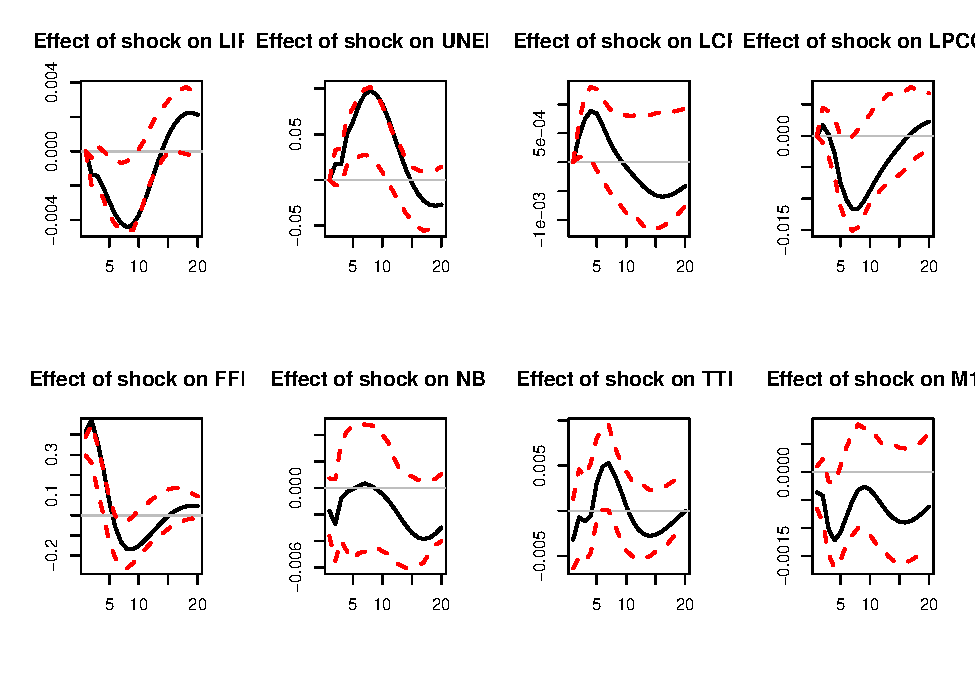
\includegraphics[width=0.95\linewidth]{IdentifStructShocks_files/figure-latex/inference4-1} \caption{Simulated IRF associated with a monetary policy shock.}\label{fig:inference4}
\end{figure}

\begin{Shaded}
\begin{Highlighting}[]
\NormalTok{IRFs.small.sample }\OtherTok{\textless{}{-}}\NormalTok{ res.svar.small.sample}\SpecialCharTok{$}\NormalTok{IRFs}
\NormalTok{median.IRFs.small.sample }\OtherTok{\textless{}{-}}\NormalTok{ res.svar.small.sample}\SpecialCharTok{$}\NormalTok{all.CI.median}
\NormalTok{simulated.IRFs.small.sample }\OtherTok{\textless{}{-}}\NormalTok{ res.svar.small.sample}\SpecialCharTok{$}\NormalTok{simulated.IRFs}
\end{Highlighting}
\end{Shaded}

\begin{Shaded}
\begin{Highlighting}[]
\CommentTok{\# True IRFs}
\NormalTok{res.svar.ordering }\OtherTok{\textless{}{-}}
  \FunctionTok{svar.ordering.2}\NormalTok{(y,}\AttributeTok{p=}\DecValTok{3}\NormalTok{,}
                  \AttributeTok{posit.of.shock =} \DecValTok{5}\NormalTok{,}
                  \AttributeTok{nb.periods.IRF =} \DecValTok{20}\NormalTok{,}
                  \AttributeTok{inference =} \DecValTok{0}\NormalTok{,}\CommentTok{\# 0 {-}\textgreater{} no inference, 1 {-}\textgreater{} parametric bootstr.,}
                  \CommentTok{\# 2 \textless{}{-} non{-}parametric bootstrap, 3 \textless{}{-} monte carlo,}
                  \CommentTok{\# 4 \textless{}{-} bootstrap{-}after{-}bootstrap}
                  \AttributeTok{indic.plot =} \DecValTok{0} \CommentTok{\# Plots are displayed if = 1.}
\NormalTok{  )}
\NormalTok{IRFs.ordering.true }\OtherTok{\textless{}{-}}\NormalTok{ res.svar.ordering}\SpecialCharTok{$}\NormalTok{IRFs}

\CommentTok{\# Distribution of coefficients resulting from the small sample VAR}
\NormalTok{h }\OtherTok{\textless{}{-}} \DecValTok{5}
\FunctionTok{par}\NormalTok{(}\AttributeTok{mfrow=}\FunctionTok{c}\NormalTok{(}\DecValTok{2}\NormalTok{,}\FunctionTok{ifelse}\NormalTok{(}\FunctionTok{round}\NormalTok{(n}\SpecialCharTok{/}\DecValTok{2}\NormalTok{)}\SpecialCharTok{==}\NormalTok{n}\SpecialCharTok{/}\DecValTok{2}\NormalTok{,n}\SpecialCharTok{/}\DecValTok{2}\NormalTok{,(n}\SpecialCharTok{+}\DecValTok{1}\NormalTok{)}\SpecialCharTok{/}\DecValTok{2}\NormalTok{)))}
\ControlFlowTok{for}\NormalTok{ (i }\ControlFlowTok{in} \DecValTok{1}\SpecialCharTok{:}\NormalTok{n)\{}
  \FunctionTok{hist}\NormalTok{(simulated.IRFs.small.sample[h,i,],}\AttributeTok{xlab=}\StringTok{""}\NormalTok{,}\AttributeTok{ylab=}\StringTok{""}\NormalTok{,}
       \AttributeTok{main=}\FunctionTok{paste}\NormalTok{(}\StringTok{"Effect at h = "}\NormalTok{,h,}\StringTok{" on "}\NormalTok{,}
\NormalTok{                  considered.variables[i],}\AttributeTok{sep=}\StringTok{""}\NormalTok{),}\AttributeTok{cex.main=}\NormalTok{.}\DecValTok{9}\NormalTok{)}
  \FunctionTok{lines}\NormalTok{(}\FunctionTok{array}\NormalTok{(}\FunctionTok{c}\NormalTok{(IRFs.small.sample[h,i],}
\NormalTok{                IRFs.small.sample[h,i],}\DecValTok{0}\NormalTok{,}\DecValTok{100}\NormalTok{),}\FunctionTok{c}\NormalTok{(}\DecValTok{2}\NormalTok{,}\DecValTok{2}\NormalTok{)),}\AttributeTok{col=}\StringTok{"red"}\NormalTok{)}
  \FunctionTok{lines}\NormalTok{(}\FunctionTok{array}\NormalTok{(}\FunctionTok{c}\NormalTok{(median.IRFs.small.sample[h,i],}
\NormalTok{                median.IRFs.small.sample[h,i],}\DecValTok{0}\NormalTok{,}\DecValTok{100}\NormalTok{),}\FunctionTok{c}\NormalTok{(}\DecValTok{2}\NormalTok{,}\DecValTok{2}\NormalTok{)),}\AttributeTok{col=}\StringTok{"blue"}\NormalTok{)}
  \FunctionTok{lines}\NormalTok{(}\FunctionTok{array}\NormalTok{(}\FunctionTok{c}\NormalTok{(IRFs.ordering.true[h,i],}
\NormalTok{                IRFs.ordering.true[h,i],}\DecValTok{0}\NormalTok{,}\DecValTok{100}\NormalTok{),}\FunctionTok{c}\NormalTok{(}\DecValTok{2}\NormalTok{,}\DecValTok{2}\NormalTok{)),}\AttributeTok{col=}\StringTok{"black"}\NormalTok{)}
  \FunctionTok{text}\NormalTok{(IRFs.small.sample[h,i],}\DecValTok{25}\NormalTok{,}\AttributeTok{label=}\StringTok{"Estimated coef."}\NormalTok{,}\AttributeTok{col=}\StringTok{"red"}\NormalTok{)}
  \FunctionTok{text}\NormalTok{(IRFs.ordering.true[h,i],}\DecValTok{30}\NormalTok{,}\AttributeTok{label=}\StringTok{"True coef."}\NormalTok{,}\AttributeTok{col=}\StringTok{"black"}\NormalTok{)}
\NormalTok{\}}
\end{Highlighting}
\end{Shaded}

\begin{figure}
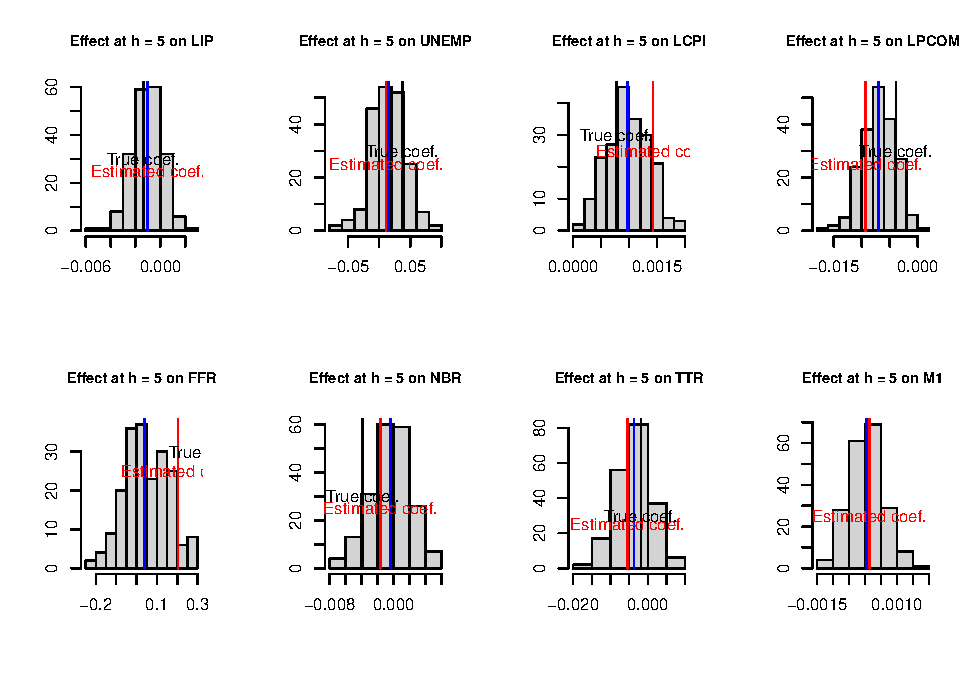
\includegraphics[width=0.95\linewidth]{IdentifStructShocks_files/figure-latex/inference5-1} \caption{IRF associated with a monetary policy shock; sign-restriction approach.}\label{fig:inference5}
\end{figure}

The main idea of the bootstrap-after-bootstrap of \citet{Kilian_1998} is to run two consecutive boostraps: the objective of the first is to compute the bias, which can further be used to correct the initial estimates of the \(\Phi_i\)'s. Further, these corrected estimates are used ---in the second boostrap--- to compute a set of IRFs (as in the standard boostrap).

More formally, the algorithm is as follows:

\begin{enumerate}
\def\labelenumi{\arabic{enumi}.}
\tightlist
\item
  Estimate the SVAR coefficients \(\{\widehat{\Phi}_j\}_{j=1,..,p}\) and \(\widehat{\Omega}\)
\item
  \textbf{First bootstrap.} For each iteration \(k\):
\end{enumerate}

\begin{enumerate}
\def\labelenumi{\alph{enumi}.}
\tightlist
\item
  Construct a sample
  \[
  y_t^{(k)}=\widehat{\Phi}_1 y_{t-1}^{(k)} + \dots + \widehat{\Phi}_p y_{t-p}^{(k)} + \hat\varepsilon_t^{(k)},
  \]
  with \(\hat\varepsilon_{t}^{(k)}=\hat\varepsilon_{s_t^{(k)}}\), where \(\{s_1^{(k)},..,s_T^{(k)}\}\) is a random set from \(\{1,..,T\}^T\).
\item
  Re-estimate the VAR and compute the coefficients \(\{\widehat{\Phi}_j\}_{j=1,..,p}^{(k)}\).
\end{enumerate}

\begin{enumerate}
\def\labelenumi{\arabic{enumi}.}
\setcounter{enumi}{2}
\tightlist
\item
  Perform \(N\) replications and compute the median coefficients \(\{\widehat{\Phi}_j\}_{j=1,..,p}^*\).
\item
  Approximate the bias terms by \(\widehat{\Theta}_j=\widehat{\Phi}_j^*-\widehat{\Phi}_j\).
\item
  Construct the bias-corrected terms \(\widetilde{\Phi}_j=\widehat{\Phi}_j-\widehat{\Theta}_j\).
\item
  \textbf{Second bootstrap.} For each iteration \(k\):
\end{enumerate}

\begin{enumerate}
\def\labelenumi{\alph{enumi}.}
\tightlist
\item
  Construct a sample now from
  \[
  y_t^{(k)}=\widetilde{\Phi}_1 y_{t-1}^{(k)} + \dots + \widetilde{\Phi}_p y_{t-p}^{(k)} + \hat\varepsilon_t^{(k)}.
  \]
\item
  Re-estimate the VAR and compute the coefficients \(\{\widehat{\Phi}^*_j\}_{j=1,..,p}^{(k)}\).
\item
  Construct the bias-corrected estimates \(\widetilde{\Phi}_j^{*(k)}=\widehat{\Phi}_j^{*(k)}-\widehat{\Theta}_j\).
\item
  Compute the associated IRFs \(\{\widetilde{\Psi}_j^{*(k)}\}_{j\ge 1}\).
\end{enumerate}

\begin{enumerate}
\def\labelenumi{\arabic{enumi}.}
\setcounter{enumi}{6}
\tightlist
\item
  Perform \(N\) replications and compute the median and the confidence interval of the set of IRFs.
\end{enumerate}

It should be noted that correcting for the bias can generate non-stationary results (\(\tilde \Phi\) with eigenvalue with modulus \(>1\)). Solution (\citet{Kilian_1998}):

In step 5, check if the largest eigenvalue of \(\tilde\Phi\) is of modulus \textless1.
If not, shrink the bias: for all \(j\)s, set \(\widehat{\Theta}_j^{(i+1)}=\delta_{i+1}\widehat{\Theta}_j^{(i)}\), with \(\delta_{i+1}=\delta_i-0.01\), starting with \(\delta_1=1\) and \(\widehat{\Theta}_j^{(1)} =\widehat{\Theta}_j\), and compute \(\widetilde{\Phi}_j^{(i+1)}=\widehat{\Phi}_j-\widehat{\Theta}_j^{(i+1)}\) until the largest eigenvalue of \(\tilde\Phi^{(i+1)}\) has modulus \textless1.

The following code implements the bootstrap-after-bootrap method.

\begin{Shaded}
\begin{Highlighting}[]
\FunctionTok{library}\NormalTok{(IdSS);}\FunctionTok{library}\NormalTok{(vars);}\FunctionTok{library}\NormalTok{(Matrix)}
\FunctionTok{data}\NormalTok{(}\StringTok{"USmonthly"}\NormalTok{)}
\NormalTok{First.date }\OtherTok{\textless{}{-}} \StringTok{"1965{-}01{-}01"}
\NormalTok{Last.date }\OtherTok{\textless{}{-}} \StringTok{"1995{-}06{-}01"}
\NormalTok{indic.first }\OtherTok{\textless{}{-}} \FunctionTok{which}\NormalTok{(USmonthly}\SpecialCharTok{$}\NormalTok{DATES}\SpecialCharTok{==}\NormalTok{First.date)}
\NormalTok{indic.last  }\OtherTok{\textless{}{-}} \FunctionTok{which}\NormalTok{(USmonthly}\SpecialCharTok{$}\NormalTok{DATES}\SpecialCharTok{==}\NormalTok{Last.date)}
\NormalTok{USmonthly   }\OtherTok{\textless{}{-}}\NormalTok{ USmonthly[indic.first}\SpecialCharTok{:}\NormalTok{indic.last,]}
\NormalTok{considered.variables}\OtherTok{\textless{}{-}}\FunctionTok{c}\NormalTok{(}\StringTok{"LIP"}\NormalTok{,}\StringTok{"UNEMP"}\NormalTok{,}\StringTok{"LCPI"}\NormalTok{,}\StringTok{"LPCOM"}\NormalTok{,}\StringTok{"FFR"}\NormalTok{,}\StringTok{"NBR"}\NormalTok{,}\StringTok{"TTR"}\NormalTok{,}\StringTok{"M1"}\NormalTok{)}
\NormalTok{y }\OtherTok{\textless{}{-}} \FunctionTok{as.matrix}\NormalTok{(USmonthly[considered.variables])}
\CommentTok{\# ===================================}
\CommentTok{\# CEE with bootstrap{-}after{-}bootstrap}
\CommentTok{\# ===================================}
\NormalTok{res.svar.ordering }\OtherTok{\textless{}{-}}
  \FunctionTok{svar.ordering.2}\NormalTok{(y,}\AttributeTok{p=}\DecValTok{3}\NormalTok{,}
                  \AttributeTok{posit.of.shock =} \DecValTok{5}\NormalTok{,}
                  \AttributeTok{nb.periods.IRF =} \DecValTok{20}\NormalTok{,}
                  \AttributeTok{inference =} \DecValTok{4}\NormalTok{,}\CommentTok{\# 0 {-}\textgreater{} no inference, 1 {-}\textgreater{} parametric bootstr.,}
                  \CommentTok{\# 2 \textless{}{-} non{-}parametric bootstrap, 3 \textless{}{-} monte carlo,}
                  \CommentTok{\# 4 \textless{}{-} bootstrap{-}after{-}bootstrap}
                  \AttributeTok{nb.draws =} \DecValTok{200}\NormalTok{,}
                  \AttributeTok{confidence.interval =} \FloatTok{0.90}\NormalTok{, }\CommentTok{\# expressed in pp.}
                  \AttributeTok{indic.plot =} \DecValTok{1} \CommentTok{\# Plots are displayed if = 1.}
\NormalTok{  )}
\end{Highlighting}
\end{Shaded}

\begin{figure}
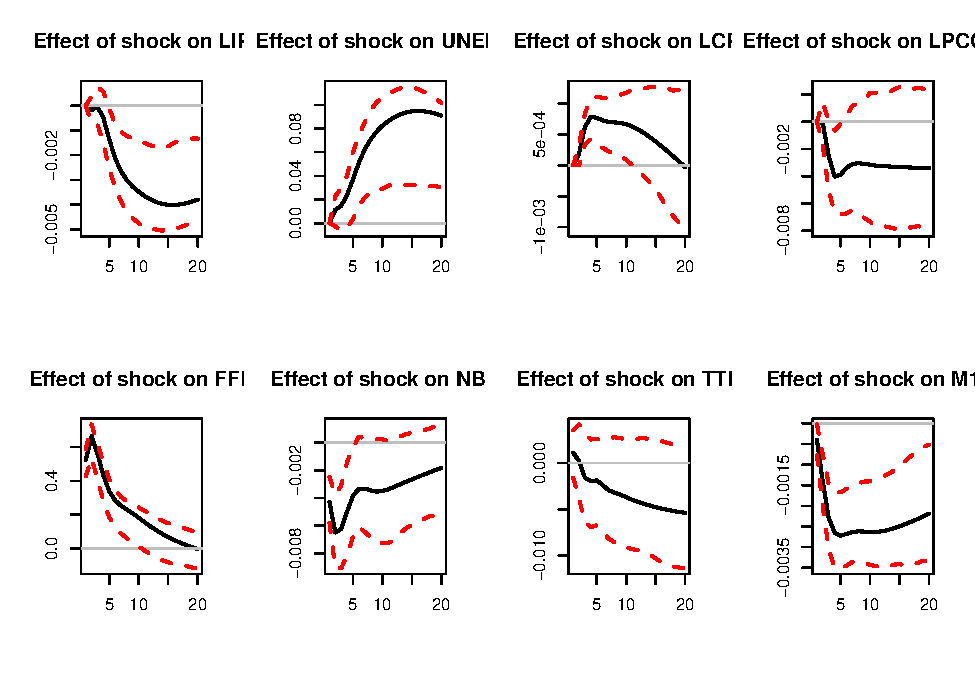
\includegraphics[width=0.95\linewidth]{IdentifStructShocks_files/figure-latex/inference6-1} \caption{IRF associated with a monetary policy shock; sign-restriction approach.}\label{fig:inference6}
\end{figure}

\begin{Shaded}
\begin{Highlighting}[]
\NormalTok{IRFs.ordering }\OtherTok{\textless{}{-}}\NormalTok{ res.svar.ordering}\SpecialCharTok{$}\NormalTok{IRFs}
\NormalTok{median.IRFs.ordering }\OtherTok{\textless{}{-}}\NormalTok{ res.svar.ordering}\SpecialCharTok{$}\NormalTok{all.CI.median}
\NormalTok{simulated.IRFs.ordering }\OtherTok{\textless{}{-}}\NormalTok{ res.svar.ordering}\SpecialCharTok{$}\NormalTok{simulated.IRFs}
\end{Highlighting}
\end{Shaded}

As an alternative, function \texttt{VAR.Boot} of package \texttt{VAR.etp} (\citet{VARetp}) can be used to operate the bias-correction approach of \citet{Kilian_1998}:

\begin{Shaded}
\begin{Highlighting}[]
\FunctionTok{library}\NormalTok{(VAR.etp)}
\FunctionTok{library}\NormalTok{(vars) }\CommentTok{\#standard VAR models}
\FunctionTok{data}\NormalTok{(dat) }\CommentTok{\# part of VAR.etp package}
\NormalTok{corrected }\OtherTok{\textless{}{-}} \FunctionTok{VAR.Boot}\NormalTok{(dat,}\AttributeTok{p=}\DecValTok{2}\NormalTok{,}\AttributeTok{nb=}\DecValTok{200}\NormalTok{,}\AttributeTok{type=}\StringTok{"const"}\NormalTok{)}
\NormalTok{noncorrec }\OtherTok{\textless{}{-}} \FunctionTok{VAR}\NormalTok{(dat,}\AttributeTok{p=}\DecValTok{2}\NormalTok{)}
\FunctionTok{rbind}\NormalTok{(corrected}\SpecialCharTok{$}\NormalTok{coef[}\DecValTok{1}\NormalTok{,],}
\NormalTok{      (corrected}\SpecialCharTok{$}\NormalTok{coef}\SpecialCharTok{+}\NormalTok{corrected}\SpecialCharTok{$}\NormalTok{Bias)[}\DecValTok{1}\NormalTok{,],}
\NormalTok{      noncorrec}\SpecialCharTok{$}\NormalTok{varresult}\SpecialCharTok{$}\NormalTok{inv}\SpecialCharTok{$}\NormalTok{coefficients)}
\end{Highlighting}
\end{Shaded}

\begin{verbatim}
##         inv(-1)   inc(-1)  con(-1)    inv(-2)   inc(-2)   con(-2)       const
## [1,] -0.3132857 0.1314415 1.050329 -0.1414933 0.1280539 0.8938500 -0.01847158
## [2,] -0.3196310 0.1459888 0.961219 -0.1605511 0.1146050 0.9343938 -0.01672199
## [3,] -0.3196310 0.1459888 0.961219 -0.1605511 0.1146050 0.9343938 -0.01672199
\end{verbatim}

\chapter{Sign restrictions}\label{Signs}

To identifiy the structural shocks, we need to find a matrix \(B\) that satisfies \(\Omega = BB'\) (with \(\Omega = \mathbb{V}ar(\varepsilon_t)\)) and other restrictions. Indeed, as explained above, \(\Omega = BB'\) is not sufficient to identify \(B\) since, if we take any orthogonal matrix \(Q\) (see Def. \ref{def:orthogonal}), then \(\mathcal{P}=BQ\) also satisfies \(\Omega = \mathcal{P}\mathcal{P}'\).

\begin{definition}[Orthogonal matrix]
\protect\hypertarget{def:orthogonal}{}\label{def:orthogonal}An orthogonal matrix \(Q\) is a matrix such that \(QQ' = I,\) i.e., all columns (rows) of \(Q\) are are
orthogonal and unit vectors:
\[q_i'q_j=0\text{ if }i\neq j\text{ and }q_i'q_j=1\text{ if }i= j,\]
where \(q_i\) is the \(i^{th}\) column of \(Q\).
\end{definition}

\section{The approach}\label{the-approach}

The idea behind the sign-restriction approach is to ``draw'' random matrices \(\mathcal{P}\) that satisfy \(\Omega = \mathcal{P}\mathcal{P}'\), and then to constitute a set of admissible matrices, keeping in this set only the simulated \(\mathcal{P}\) matrices that satisfy some predefined sign-based restriction. An example of restriction is ``\emph{after one year, a contractionary monetary-policy shocks has a negative impact on inflation}''.

As suggested above, if \(B\) is any matrix that satisfies \(\Omega = BB'\) (for instance, \(B\) can be based on the Cholesky decomposition of \(\Omega\)), then we also have \(\Omega = \mathcal{P}\mathcal{P}'\) as soon as \(\mathcal{P}=BQ\), where \(Q\) is an orthogonal matrix. Therefore, to draw \(\mathcal{P}\) matrices, it suffices to draw in the set of orthogonal matrices.

To fix ideas, consider dimension 2. In that case, the orthogonal matrices are rotation matrices, and the set of orthogonal matrices can be parameterized by the angle \(x\), with:
\[
Q_x=\begin{pmatrix}\cos(x)&\cos\left(x+\frac{\pi}{2}\right)\\
\sin(x)&\sin\left(x+\frac{\pi}{2}\right)\end{pmatrix}=\begin{pmatrix}\cos(x)&-\sin(x)\\
\sin(x)&\cos(x)\end{pmatrix}.
\]
(This is an angle-\(x\) counter-clockwise rotation.) Hence, in that case, by drawing \(x\) randomly from \([0,2\pi]\), we draw randomly from the set of \(2\times2\) rotation matrices. For high-dimensional VAR, we lose this simple geometrical representation, though. It is not always possible to parametrize a rotation matrix (high-dimensional VARs).

How to proceed, then? \citet{Arias_et_al_2018} provide a procedure. Their approach is based on the so-called \(QR\) decomposition: any square matrix \(X\) may be decomposed as \(X=QR\) where \(Q\) is an orthogonal matrix and \(R\) is an upper diagonal matrix. With this in mind, they propose a two-step approach:

\begin{enumerate}
\def\labelenumi{\roman{enumi}.}
\tightlist
\item
  Draw a random matrix \(X\) by drawing each element from independent standard normal distribution.
\item
  Let \(X = QR\) be the \(QR\) decomposition of \(X\) with the diagonal of \(R\) normalized to be
  positive. The random matrix \(Q\) is orthogonal and is a draw from the uniform distribution over the set of orthogonal matrices.
\end{enumerate}

Equipped with this procedure, the sign-restriction is based on the following algorithm:

\begin{enumerate}
\def\labelenumi{\arabic{enumi}.}
\tightlist
\item
  Draw a random orthogonal matrix \(Q\) (using step i. and ii. described above).
\item
  Compute \(B = PQ\) where \(P\) is the Cholesky decomposition of the reduced form residuals \(\Omega_{\varepsilon}\).
\item
  Compute the impulse response associated with \(B\) \(y_{t,t+k}=\Phi^kB\) or the cumulated response \(\bar y_{t,t+k}=\sum_{j=0}^{k}\Phi^jB\).
\item
  Are the sign restrictions satisfied?
\end{enumerate}

\begin{enumerate}
\def\labelenumi{\alph{enumi}.}
\tightlist
\item
  \textbf{Yes}. Store the impulse response in the set of admissible response.
\item
  \textbf{No}. Discard the impulse response.
\end{enumerate}

\begin{enumerate}
\def\labelenumi{\arabic{enumi}.}
\setcounter{enumi}{4}
\tightlist
\item
  Perform \(N\) replications and report the median impulse response (and its ``confidence'' intervals).
\end{enumerate}

Note: to take into account the uncertainty in \(B\) and \(\Phi\), you can draw \(B\) and \(\Phi\) in Steps 2 and 3 using an inference method (see Section \ref{Inference}).

The sign-restriction approach method has the advantage of being relatively agnostic. Moreover, it is fairly flexible, as one can impose sign restrictions on any variable, at any horizon.

\section{An example}\label{an-example}

A prominent example is \citet{Uhlig_2005}. Using US monthly data from 1965.I to 2003.XII, he employs sign restrictions to estimate the effect of monetary policy shocks.

According to conventional wisdom, monetary contractions should:\footnote{Standard identification schemes often fail to achieve these 4 points. Two puzzles regularly arise: \emph{liquidity puzzle}: when identifying monetary policy shocks as surprise increases in the stock of money, interest rates tend to go up, not down; \emph{price puzzle}: after a contractionary monetary policy shock, even with interest rates going up and money supply going down, inflation goes up rather than down.}

\begin{itemize}
\tightlist
\item
  Raise the federal funds rate,
\item
  Lower prices,
\item
  Decrease non-borrowed reserves,
\item
  Reduce real output.
\end{itemize}

The restrictions considered by \citet{Uhlig_2005} are as follows: an expansionary monetary policy shock leads to:

\begin{itemize}
\tightlist
\item
  Increases in prices
\item
  Increase in nonborrowed reserves
\item
  Decreases in the federal funds rate
\end{itemize}

What about output? Since is the response of interest, we leave it un-restricted.

\begin{Shaded}
\begin{Highlighting}[]
\FunctionTok{library}\NormalTok{(IdSS);}\FunctionTok{library}\NormalTok{(vars);}\FunctionTok{library}\NormalTok{(Matrix)}
\FunctionTok{data}\NormalTok{(}\StringTok{"USmonthly"}\NormalTok{)}
\NormalTok{First.date }\OtherTok{\textless{}{-}} \StringTok{"1965{-}01{-}01"}
\NormalTok{Last.date }\OtherTok{\textless{}{-}} \StringTok{"1995{-}06{-}01"}
\NormalTok{indic.first }\OtherTok{\textless{}{-}} \FunctionTok{which}\NormalTok{(USmonthly}\SpecialCharTok{$}\NormalTok{DATES}\SpecialCharTok{==}\NormalTok{First.date)}
\NormalTok{indic.last  }\OtherTok{\textless{}{-}} \FunctionTok{which}\NormalTok{(USmonthly}\SpecialCharTok{$}\NormalTok{DATES}\SpecialCharTok{==}\NormalTok{Last.date)}
\NormalTok{USmonthly   }\OtherTok{\textless{}{-}}\NormalTok{ USmonthly[indic.first}\SpecialCharTok{:}\NormalTok{indic.last,]}
\NormalTok{considered.variables}\OtherTok{\textless{}{-}}\FunctionTok{c}\NormalTok{(}\StringTok{"LIP"}\NormalTok{,}\StringTok{"UNEMP"}\NormalTok{,}\StringTok{"LCPI"}\NormalTok{,}\StringTok{"LPCOM"}\NormalTok{,}\StringTok{"FFR"}\NormalTok{,}\StringTok{"NBR"}\NormalTok{,}\StringTok{"TTR"}\NormalTok{,}\StringTok{"M1"}\NormalTok{)}
\NormalTok{n }\OtherTok{\textless{}{-}} \FunctionTok{length}\NormalTok{(considered.variables)}
\NormalTok{y }\OtherTok{\textless{}{-}} \FunctionTok{as.matrix}\NormalTok{(USmonthly[considered.variables])}
\NormalTok{sign.restrictions }\OtherTok{\textless{}{-}} \FunctionTok{list}\NormalTok{()}
\NormalTok{horizon }\OtherTok{\textless{}{-}} \FunctionTok{list}\NormalTok{()}
\CommentTok{\#Define sign restrictions and horizon for restrictions}
\ControlFlowTok{for}\NormalTok{(i }\ControlFlowTok{in} \DecValTok{1}\SpecialCharTok{:}\NormalTok{n)\{}
\NormalTok{  sign.restrictions[[i]] }\OtherTok{\textless{}{-}} \FunctionTok{matrix}\NormalTok{(}\DecValTok{0}\NormalTok{,n,n)}
\NormalTok{  horizon[[i]] }\OtherTok{\textless{}{-}} \DecValTok{1}
\NormalTok{\}}
\CommentTok{\# Sign restrictions on shock 1 (monetary shock)}
\NormalTok{sign.restrictions[[}\DecValTok{1}\NormalTok{]][}\DecValTok{1}\NormalTok{,}\DecValTok{3}\NormalTok{] }\OtherTok{\textless{}{-}} \DecValTok{1}  \CommentTok{\# positive impact on price level}
\NormalTok{sign.restrictions[[}\DecValTok{1}\NormalTok{]][}\DecValTok{2}\NormalTok{,}\DecValTok{5}\NormalTok{] }\OtherTok{\textless{}{-}} \SpecialCharTok{{-}}\DecValTok{1} \CommentTok{\# negative impact on interest rate}
\NormalTok{sign.restrictions[[}\DecValTok{1}\NormalTok{]][}\DecValTok{3}\NormalTok{,}\DecValTok{6}\NormalTok{] }\OtherTok{\textless{}{-}} \DecValTok{1} \CommentTok{\# positive impact on non{-}borrowed reserves}
\NormalTok{horizon[[}\DecValTok{1}\NormalTok{]] }\OtherTok{\textless{}{-}} \DecValTok{1}\SpecialCharTok{:}\DecValTok{5} \CommentTok{\# from horizon 1 to 5}
\NormalTok{res.svar.signs }\OtherTok{\textless{}{-}} 
  \FunctionTok{svar.signs}\NormalTok{(y,}\AttributeTok{p=}\DecValTok{3}\NormalTok{,}
             \AttributeTok{nb.shocks =} \DecValTok{1}\NormalTok{, }\CommentTok{\#number of identified shocks}
             \AttributeTok{nb.periods.IRF =} \DecValTok{20}\NormalTok{,}
             \AttributeTok{bootstrap.replications =} \DecValTok{1}\NormalTok{, }\CommentTok{\# = 1 if no bootstrap, = N if bootstrap}
             \AttributeTok{confidence.interval =} \FloatTok{0.90}\NormalTok{, }\CommentTok{\# expressed in pp.}
             \AttributeTok{indic.plot =} \DecValTok{1}\NormalTok{, }\CommentTok{\# Plots are displayed if = 1.}
             \AttributeTok{nb.draws =} \DecValTok{10000}\NormalTok{, }\CommentTok{\# number of draws}
\NormalTok{             sign.restrictions,}
\NormalTok{             horizon,}
             \AttributeTok{recursive =}\DecValTok{1} \CommentTok{\#  =0 \textless{}{-} draw Q directly, =1 \textless{}{-} draw q recursively}
\NormalTok{  )}
\end{Highlighting}
\end{Shaded}

\begin{figure}
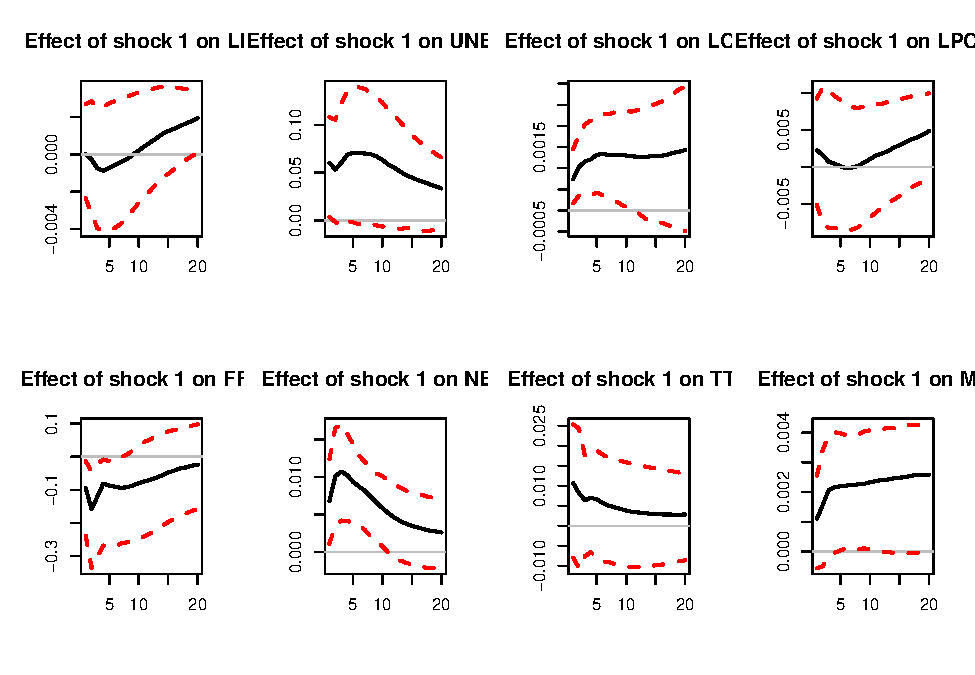
\includegraphics[width=0.95\linewidth]{IdentifStructShocks_files/figure-latex/signrestr1-1} \caption{IRF associated with a monetary policy shock; sign-restriction approach.}\label{fig:signrestr1}
\end{figure}

\begin{Shaded}
\begin{Highlighting}[]
\CommentTok{\# Output}
\NormalTok{IRFs.signs }\OtherTok{\textless{}{-}}\NormalTok{ res.svar.signs}\SpecialCharTok{$}\NormalTok{IRFs.signs }\CommentTok{\# all the simulated IRFs}
\NormalTok{nb.rotations }\OtherTok{\textless{}{-}}\NormalTok{ res.svar.signs}\SpecialCharTok{$}\NormalTok{xx }\CommentTok{\# total number of rotations}
\NormalTok{all.CI.median }\OtherTok{\textless{}{-}}\NormalTok{ res.svar.signs}\SpecialCharTok{$}\NormalTok{all.CI.median }\CommentTok{\# median IRFs for the selected shocks}
\NormalTok{all.CI.lower.bounds }\OtherTok{\textless{}{-}}\NormalTok{ res.svar.signs}\SpecialCharTok{$}\NormalTok{all.CI.lower.bounds }\CommentTok{\# lower{-}bound IRFs for the selected shocks}
\NormalTok{all.CI.upper.bounds }\OtherTok{\textless{}{-}}\NormalTok{ res.svar.signs}\SpecialCharTok{$}\NormalTok{all.CI.upper.bounds }\CommentTok{\# upper{-}bound IRFs for the selected shocks}
\end{Highlighting}
\end{Shaded}

It has to be stressed that the sign restriction approach does not lead to a unique IRF, but to a set of admissible IRFs. Accordingly, we say that this approach is set-identified, not point-identified.

\section{The penalty-function approach (PFA)}\label{the-penalty-function-approach-pfa}

An alternative approach is the so-called \textbf{penalty-function approach} (PFA, \citet{Uhlig_2005}, present in \citet{Danne_2015}'s package). This approach relies on a \emph{penalty function}:
\[
f(x)=
\begin{cases}
x, & \text{if } x \le 0,\\[6pt]
100x, & \text{if } x > 0.
\end{cases}
\]

which penalizes positive responses and rewards negative responses.

Let \(\psi_k^j(q)\) be the impulse response of variable \(j\). The \(\psi_k^j(q)\)'s are the elements of \(\psi_k(q)=\Psi_kq\).

Let \(\sigma_j\) be the standard deviation of variable \(j\). Let \(\iota_{j,k}=1\) if we restrict the response of variable \(j\) at the \(k^th\) horizon to be negative, \(\iota_{j,k}=-1\) if we restrict it to be positive, and \(\iota_{j,k}=0\) if there is no restriction. The total penalty is given by \[
\mathbf{P}(q)=\sum_{j=1}^m\sum_{k=0}^Kf\left(\iota_{j,k}\frac{\psi_k^j(q)}{\sigma_j}\right).
\]

We are looking for a solution to
\[\begin{array}{ll}
&\min_q \mathbf{P}(q)\\
\text{s.t. }&q'q=1.\end{array}\]

The problem is solved numerically.

\section{Narrative sign restrictions}\label{NarrativeSign}

A related approach, introduced by \citet{AntolinDiaz_RubioRamirez_2018}, consists in imposing that, on some specific dates (based on narrative evidence), the signs of some shocks are positive (or negative).\footnote{See also Section \ref{NarrativeHistDecomp}.} For instance, \citet{AntolinDiaz_RubioRamirez_2018} argue that one should rule out structural parameters that disagree with the view that ``a negative oil supply shock occurred at the outbreak of the Gulf War in August 1990.''

Suppose we want to impose the restriction that, at dates \(\{t_1,\dots,t_J\}\), the signs of the \(j^{th}\) shock are all positive. Then, the narrative sign restrictions are simply imposed by:
\[
\hat{\eta}_{j,t}(B) = e_j'\hat\eta_{t}(B) > 0,
\]
where \(\hat\eta_{t}(B)\) is the vector of structural shock associated with a given matrix \(B\) (and where \(e_j\) is the \(j^{th}\) column of the \(n \times n\) identity matrix).

\chapter{Combining sign and zero restrictions}\label{SignsZeros}

Sometimes we need to combine different types of restrictions. For instance:

\begin{itemize}
\tightlist
\item
  One shock satisfies both zero and sign restrictions.
\item
  Some shocks can be identified with zero restrictions (SR or LR), others with sign restrictions.
\item
  Some shocks satisfy the same zero restrictions (e.g.~no LR effect on output) but can be distinguished from each other through sign restrictions.
\end{itemize}

In such instances, we must make independent draws from the set of all structural parameters satisfying the zero restrictions. How to do that? \citet{Arias_et_al_2018} propose to impose the zero restrictions on \(B\), and then check signs. Remember, \(\mathcal{P}=BQ\) is a candidate impact IRF. For each structural shock \(j\), define the \(m\)-column matrices \(Z_j\) (zero restrictions) and \(S_j\) (sign restrictions). Each row of \(Z_j\) (resp. \(S_j\)) defines a zero (resp. sign) restriction. \(Z_j\) has \(m-j\) rows at most (i.e., \(m-j\) zero restriction at most).

\begin{example}
\protect\hypertarget{exm:exMixSignSR}{}\label{exm:exMixSignSR}In a 4-variable VAR, we want to impose that the first structural shock has no effect on variable 1, affects positively variable 2 and negatively variable 3 on impact:
\[Z_1 = \begin{pmatrix}1 & 0 & 0 & 0\end{pmatrix}, \]
\[S_1 = \begin{pmatrix}0 & 1 & 0 & 0\\
0 & 0 & -1 & 0\end{pmatrix}. \]

For both zero and sign restrictions to be satisfied, we must have
\[
Z_jb_j=0 \quad \mbox{and} \quad S_jb_j>0,
\]
where \(b_j\) is the \(j^{th}\) column of \(B\), i.e.~the impact effect of the \(j^{th}\) structural shock.
\end{example}

The algorithm is as follows:

\begin{enumerate}
\def\labelenumi{\arabic{enumi}.}
\tightlist
\item
  For \(1\le j\le m\), draw \(u_j\in \mathbb{R}^{m+1-j-z_j}\) from a standard normal distribution (\(z_j\) is the number of zero restrictions imposed on the \(j^{th}\) shock) and set \(w_j = u_j/||u_j||\).
\item
  Define \(Q= \begin{pmatrix}q_1&...&q_m\end{pmatrix}\) recursively by \(q_j = K_jw_j\) for any matrix \(K_j\) whose columns form an orthogonal basis for the null space of the matrix \[M_j =
  \begin{pmatrix} q_1&...&q_{j-1}&\color{blue}{(Z_jP)'}\end{pmatrix}'.\] (Vector \(q_j\) will then be orthogonal to \(\begin{pmatrix} q_1&...&q_{j-1}\end{pmatrix}\) and satisfy the zero restriction.)
\item
  Set \(B=PQ\).
\item
  Check sign restrictions (\(S_jb_j>0\) for all \(j\)?).
\end{enumerate}

Perform \(N\) replications and report the median impulse response (and its confidence intervals).

Function \texttt{svar.signs} can run this algorithm. It is called as follows:\footnote{Note that outputs are not reported here; just copy-paste in Rstudio to get the 6 sets of IRFs.}

\begin{Shaded}
\begin{Highlighting}[]
\FunctionTok{library}\NormalTok{(IdSS);}\FunctionTok{library}\NormalTok{(vars);}\FunctionTok{library}\NormalTok{(Matrix)}
\FunctionTok{data}\NormalTok{(}\StringTok{"USmonthly"}\NormalTok{)}
\NormalTok{First.date }\OtherTok{\textless{}{-}} \StringTok{"1965{-}01{-}01"}
\NormalTok{Last.date }\OtherTok{\textless{}{-}} \StringTok{"1995{-}06{-}01"}
\NormalTok{indic.first }\OtherTok{\textless{}{-}} \FunctionTok{which}\NormalTok{(USmonthly}\SpecialCharTok{$}\NormalTok{DATES}\SpecialCharTok{==}\NormalTok{First.date)}
\NormalTok{indic.last  }\OtherTok{\textless{}{-}} \FunctionTok{which}\NormalTok{(USmonthly}\SpecialCharTok{$}\NormalTok{DATES}\SpecialCharTok{==}\NormalTok{Last.date)}
\NormalTok{USmonthly   }\OtherTok{\textless{}{-}}\NormalTok{ USmonthly[indic.first}\SpecialCharTok{:}\NormalTok{indic.last,]}
\NormalTok{considered.variables}\OtherTok{\textless{}{-}}\FunctionTok{c}\NormalTok{(}\StringTok{"LIP"}\NormalTok{,}\StringTok{"UNEMP"}\NormalTok{,}\StringTok{"LCPI"}\NormalTok{,}\StringTok{"LPCOM"}\NormalTok{,}\StringTok{"FFR"}\NormalTok{,}\StringTok{"NBR"}\NormalTok{,}\StringTok{"TTR"}\NormalTok{,}\StringTok{"M1"}\NormalTok{)}
\NormalTok{n }\OtherTok{\textless{}{-}} \FunctionTok{length}\NormalTok{(considered.variables)}
\NormalTok{y }\OtherTok{\textless{}{-}} \FunctionTok{as.matrix}\NormalTok{(USmonthly[considered.variables])}
\NormalTok{sign.restrictions }\OtherTok{\textless{}{-}} \FunctionTok{list}\NormalTok{()}
\NormalTok{SR.restrictions }\OtherTok{\textless{}{-}} \FunctionTok{list}\NormalTok{()}
\NormalTok{horizon }\OtherTok{\textless{}{-}} \FunctionTok{list}\NormalTok{()}

\CommentTok{\#Define sign restrictions and horizon for restrictions}
\ControlFlowTok{for}\NormalTok{(i }\ControlFlowTok{in} \DecValTok{1}\SpecialCharTok{:}\NormalTok{n)\{}
\NormalTok{  sign.restrictions[[i]] }\OtherTok{\textless{}{-}} \FunctionTok{matrix}\NormalTok{(}\DecValTok{0}\NormalTok{,n,n)}
\NormalTok{  horizon[[i]] }\OtherTok{\textless{}{-}} \DecValTok{1}
\NormalTok{\}}
\CommentTok{\# 2 shocks on the demand for reserves}
\NormalTok{sign.restrictions[[}\DecValTok{1}\NormalTok{]][}\DecValTok{1}\NormalTok{,}\DecValTok{6}\NormalTok{] }\OtherTok{\textless{}{-}} \DecValTok{1} 
\NormalTok{sign.restrictions[[}\DecValTok{2}\NormalTok{]][}\DecValTok{1}\NormalTok{,}\DecValTok{7}\NormalTok{] }\OtherTok{\textless{}{-}} \DecValTok{1}
\CommentTok{\# 3 shocks that drive an endogenous response of the interest rate}
\NormalTok{sign.restrictions[[}\DecValTok{3}\NormalTok{]][}\DecValTok{1}\NormalTok{,}\DecValTok{1}\NormalTok{] }\OtherTok{\textless{}{-}} \DecValTok{1}
\NormalTok{sign.restrictions[[}\DecValTok{3}\NormalTok{]][}\DecValTok{2}\NormalTok{,}\DecValTok{5}\NormalTok{] }\OtherTok{\textless{}{-}} \DecValTok{1}
\NormalTok{sign.restrictions[[}\DecValTok{4}\NormalTok{]][}\DecValTok{1}\NormalTok{,}\DecValTok{2}\NormalTok{] }\OtherTok{\textless{}{-}} \SpecialCharTok{{-}}\DecValTok{1}
\NormalTok{sign.restrictions[[}\DecValTok{4}\NormalTok{]][}\DecValTok{2}\NormalTok{,}\DecValTok{5}\NormalTok{] }\OtherTok{\textless{}{-}} \DecValTok{1}
\NormalTok{sign.restrictions[[}\DecValTok{5}\NormalTok{]][}\DecValTok{1}\NormalTok{,}\DecValTok{3}\NormalTok{] }\OtherTok{\textless{}{-}} \DecValTok{1}
\NormalTok{sign.restrictions[[}\DecValTok{5}\NormalTok{]][}\DecValTok{2}\NormalTok{,}\DecValTok{5}\NormalTok{] }\OtherTok{\textless{}{-}} \DecValTok{1}
\CommentTok{\# monetary policy shock}
\NormalTok{sign.restrictions[[}\DecValTok{6}\NormalTok{]][}\DecValTok{1}\NormalTok{,}\DecValTok{5}\NormalTok{] }\OtherTok{\textless{}{-}} \SpecialCharTok{{-}}\DecValTok{1}
\NormalTok{sign.restrictions[[}\DecValTok{6}\NormalTok{]][}\DecValTok{2}\NormalTok{,}\DecValTok{3}\NormalTok{] }\OtherTok{\textless{}{-}} \DecValTok{1}
\NormalTok{sign.restrictions[[}\DecValTok{6}\NormalTok{]][}\DecValTok{3}\NormalTok{,}\DecValTok{6}\NormalTok{] }\OtherTok{\textless{}{-}} \DecValTok{1}
\CommentTok{\# horizon for sign restrictions on monetary policy shock}
\NormalTok{horizon[[}\DecValTok{6}\NormalTok{]] }\OtherTok{\textless{}{-}} \DecValTok{1}\SpecialCharTok{:}\DecValTok{5}

\CommentTok{\#Define zero restrictions}
\CommentTok{\# 2 shocks on the demand for reserves}
\NormalTok{SR.restrictions[[}\DecValTok{1}\NormalTok{]] }\OtherTok{\textless{}{-}} \FunctionTok{array}\NormalTok{(}\DecValTok{0}\NormalTok{,}\FunctionTok{c}\NormalTok{(}\DecValTok{1}\NormalTok{,n))}
\NormalTok{SR.restrictions[[}\DecValTok{1}\NormalTok{]][}\DecValTok{1}\NormalTok{,}\DecValTok{5}\NormalTok{] }\OtherTok{\textless{}{-}} \DecValTok{1} \CommentTok{\# no impact on the interest rate}
\NormalTok{SR.restrictions[[}\DecValTok{2}\NormalTok{]] }\OtherTok{\textless{}{-}} \FunctionTok{array}\NormalTok{(}\DecValTok{0}\NormalTok{,}\FunctionTok{c}\NormalTok{(}\DecValTok{1}\NormalTok{,n))}
\NormalTok{SR.restrictions[[}\DecValTok{2}\NormalTok{]][}\DecValTok{1}\NormalTok{,}\DecValTok{5}\NormalTok{] }\OtherTok{\textless{}{-}} \DecValTok{1} \CommentTok{\# no impact on the interest rate}
\ControlFlowTok{for}\NormalTok{(i }\ControlFlowTok{in} \DecValTok{3}\SpecialCharTok{:}\NormalTok{n)\{}
\NormalTok{  SR.restrictions[[i]] }\OtherTok{\textless{}{-}} \FunctionTok{array}\NormalTok{(}\DecValTok{0}\NormalTok{,}\FunctionTok{c}\NormalTok{(}\DecValTok{0}\NormalTok{,n))}
\NormalTok{\}}

\NormalTok{res.svar.signs.zeros }\OtherTok{\textless{}{-}} \FunctionTok{svar.signs}\NormalTok{(y,}\AttributeTok{p=}\DecValTok{3}\NormalTok{,}
                                  \AttributeTok{nb.shocks =} \DecValTok{6}\NormalTok{, }\CommentTok{\#number of identified shocks}
                                  \AttributeTok{nb.periods.IRF =} \DecValTok{20}\NormalTok{,}
                                  \AttributeTok{bootstrap.replications =} \DecValTok{100}\NormalTok{, }\CommentTok{\# = 1 if no bootstrap, = N if bootstrap}
                                  \AttributeTok{confidence.interval =} \FloatTok{0.90}\NormalTok{, }\CommentTok{\# expressed in pp.}
                                  \AttributeTok{indic.plot =} \DecValTok{1}\NormalTok{, }\CommentTok{\# Plots are displayed if = 1.}
                                  \AttributeTok{nb.draws =} \DecValTok{10000}\NormalTok{, }\CommentTok{\# number of draws}
\NormalTok{                                  sign.restrictions,}
\NormalTok{                                  horizon,}
                                  \AttributeTok{recursive =}\DecValTok{0}\NormalTok{,}
\NormalTok{                                  SR.restrictions}
\NormalTok{)}
\end{Highlighting}
\end{Shaded}

\begin{figure}
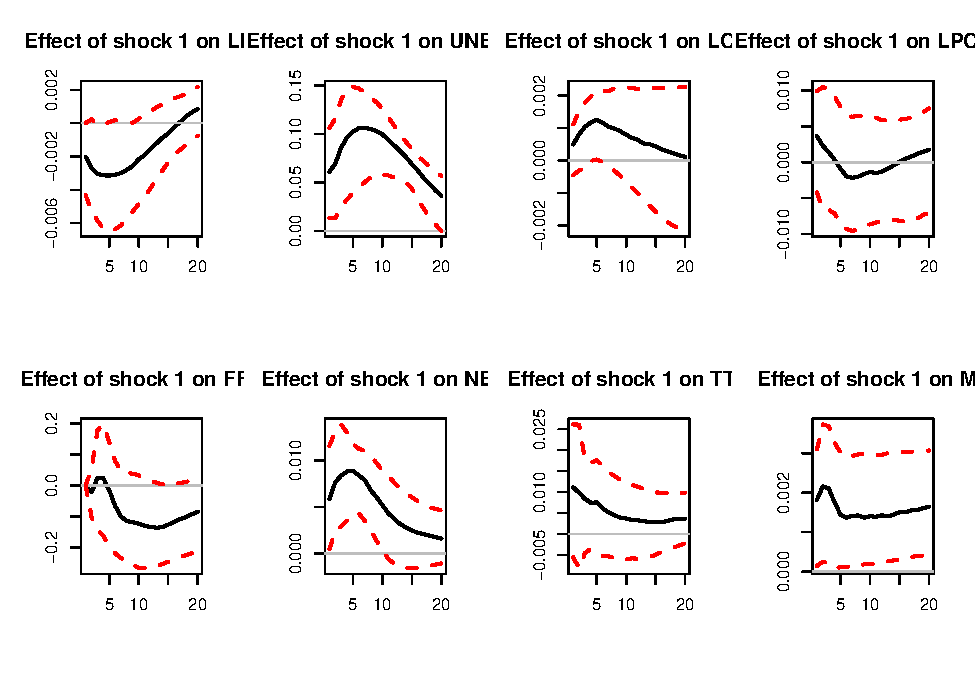
\includegraphics[width=0.95\linewidth]{IdentifStructShocks_files/figure-latex/signrestr2-1} \caption{IRFs; sign-restriction approach.}\label{fig:signrestr2-1}
\end{figure}
\begin{figure}
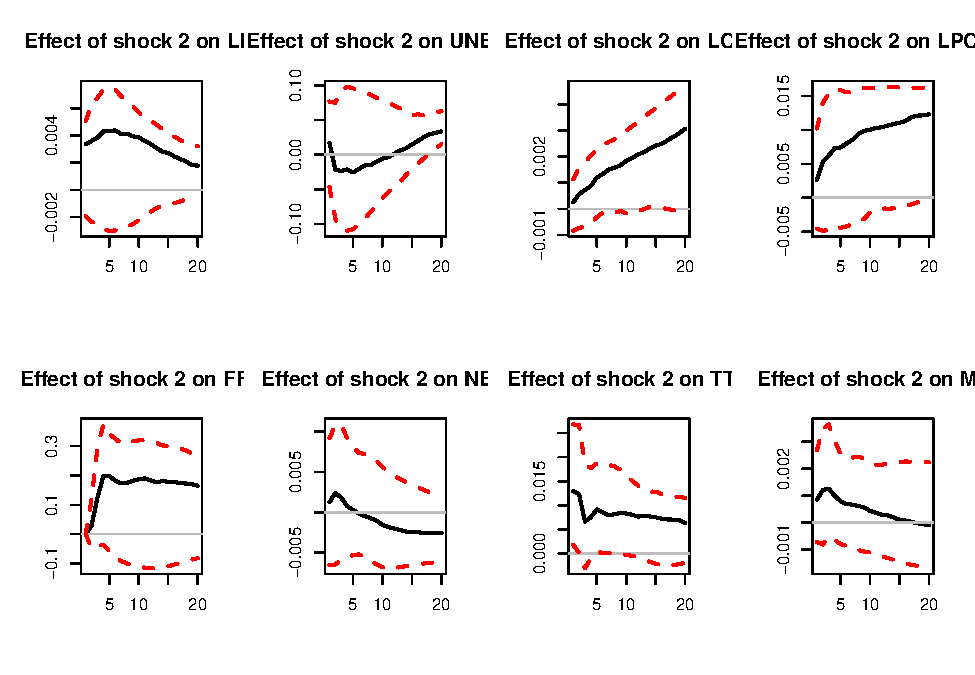
\includegraphics[width=0.95\linewidth]{IdentifStructShocks_files/figure-latex/signrestr2-2} \caption{IRFs; sign-restriction approach.}\label{fig:signrestr2-2}
\end{figure}
\begin{figure}
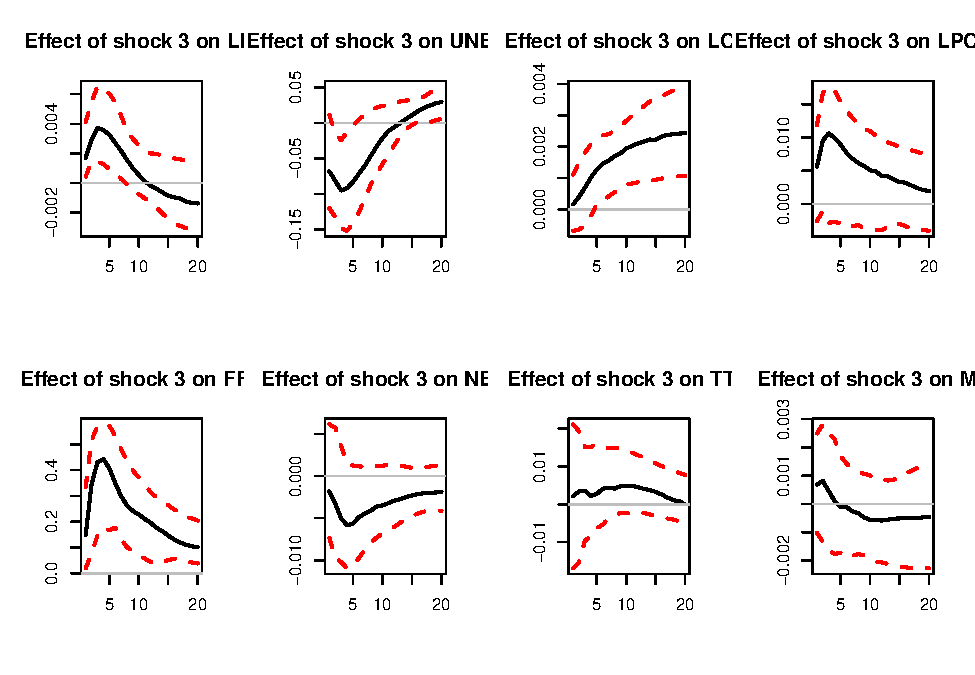
\includegraphics[width=0.95\linewidth]{IdentifStructShocks_files/figure-latex/signrestr2-3} \caption{IRFs; sign-restriction approach.}\label{fig:signrestr2-3}
\end{figure}
\begin{figure}
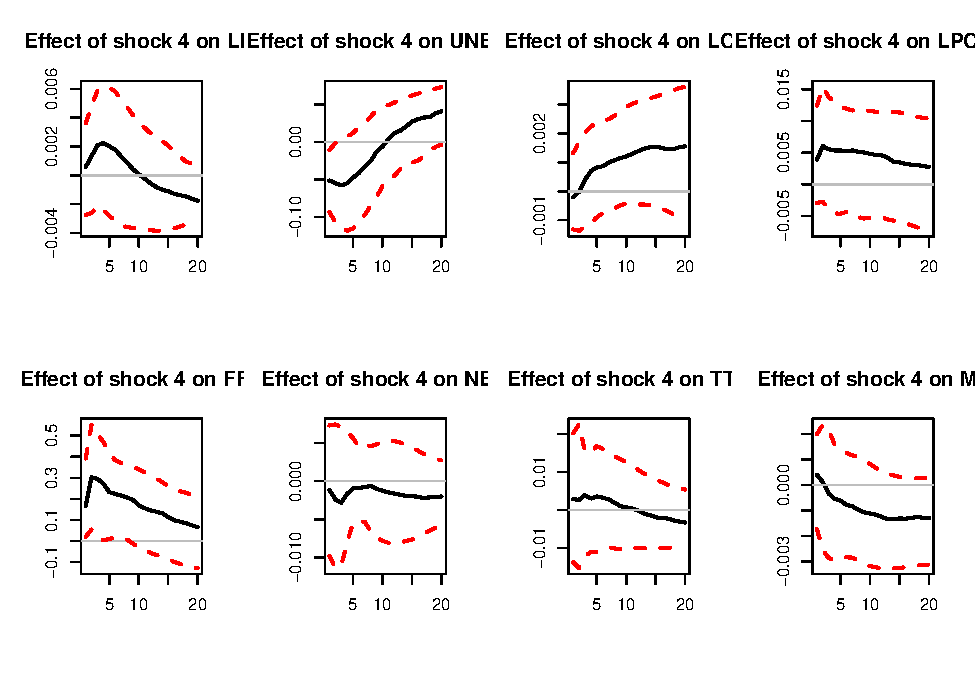
\includegraphics[width=0.95\linewidth]{IdentifStructShocks_files/figure-latex/signrestr2-4} \caption{IRFs; sign-restriction approach.}\label{fig:signrestr2-4}
\end{figure}
\begin{figure}
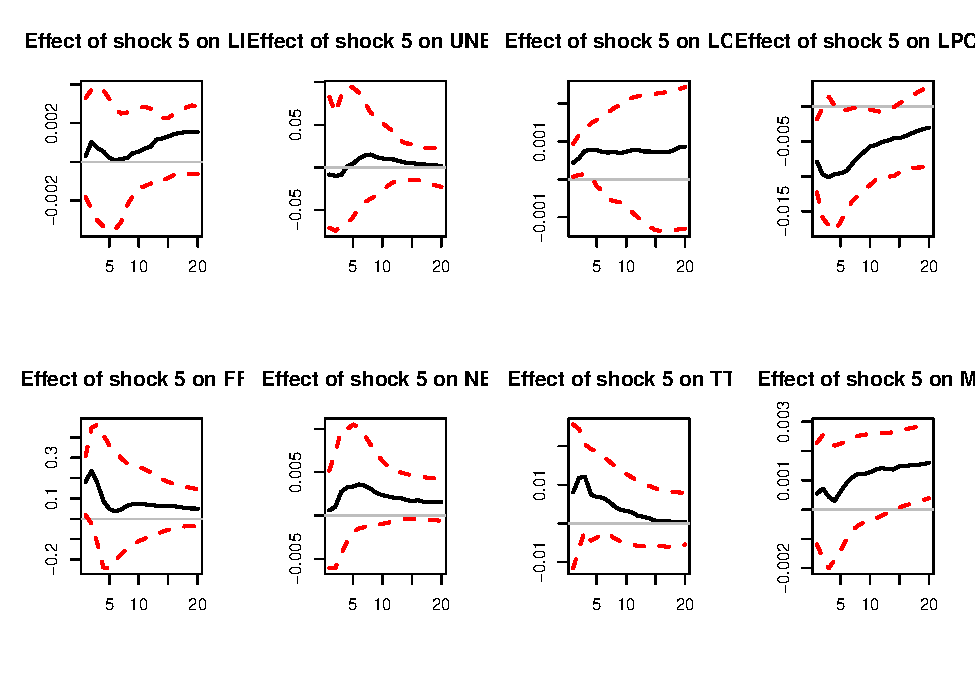
\includegraphics[width=0.95\linewidth]{IdentifStructShocks_files/figure-latex/signrestr2-5} \caption{IRFs; sign-restriction approach.}\label{fig:signrestr2-5}
\end{figure}
\begin{figure}
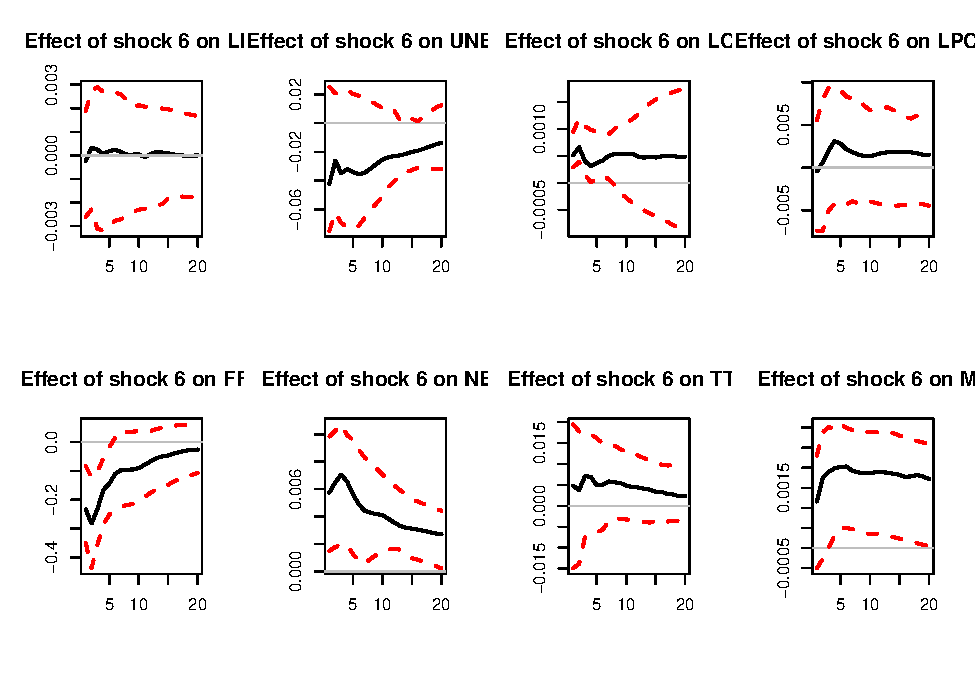
\includegraphics[width=0.95\linewidth]{IdentifStructShocks_files/figure-latex/signrestr2-6} \caption{IRFs; sign-restriction approach.}\label{fig:signrestr2-6}
\end{figure}

\begin{Shaded}
\begin{Highlighting}[]
\CommentTok{\# Output}
\NormalTok{IRFs.signs }\OtherTok{\textless{}{-}}\NormalTok{ res.svar.signs.zeros}\SpecialCharTok{$}\NormalTok{IRFs.signs }\CommentTok{\# all the simulated IRFs}
\NormalTok{nb.rotations }\OtherTok{\textless{}{-}}\NormalTok{ res.svar.signs.zeros}\SpecialCharTok{$}\NormalTok{xx }\CommentTok{\# total number of rotations}
\NormalTok{all.CI.median }\OtherTok{\textless{}{-}}\NormalTok{ res.svar.signs.zeros}\SpecialCharTok{$}\NormalTok{all.CI.median }\CommentTok{\# median IRFs for the selected shocks}
\NormalTok{all.CI.lower.bounds }\OtherTok{\textless{}{-}}\NormalTok{ res.svar.signs.zeros}\SpecialCharTok{$}\NormalTok{all.CI.lower.bounds }\CommentTok{\# lower{-}bound IRFs for the selected shocks}
\NormalTok{all.CI.upper.bounds }\OtherTok{\textless{}{-}}\NormalTok{ res.svar.signs.zeros}\SpecialCharTok{$}\NormalTok{all.CI.upper.bounds }\CommentTok{\# upper{-}bound IRFs for the selected shocks}
\end{Highlighting}
\end{Shaded}

\chapter{Forecast error variance maximization}\label{forecast-error-variance-maximization}

\section{The main (unconditional) approach}\label{the-main-unconditional-approach}

The approach presented in this section exploits the derivations of \citet{Uhlig_2004}.

Consider a process \(\{y_t\}\) that admits the infinite MA representation of Eq. \eqref{eq:InfMA}. Let \(Q\) be an orthogonal matrix, an alternative decomposition of \(y_t\) is:
\begin{eqnarray}
y_t&=&\sum_{h=0}^{+\infty}\Psi_h\underbrace{\eta_{t-h}}_{Q\tilde \eta_{t-h}} = \sum_{h=0}^{+\infty}\underbrace{\Psi_hQ}_{\tilde\Psi_h}\tilde
\eta_{t-h} = \sum_{h=0}^{+\infty}\tilde\Psi_h\tilde \eta_{t-h},
\end{eqnarray}
where \(\tilde \eta_{t-h}=Q'\eta_{t-h}\) are the white-noise shocks associated with the new MA representation, \(Q\) being an orthgonal matrix. (They also satisfy \(\mathbb{V}ar(\tilde\eta_t)=Id\).)

The \(h\)-step ahead prediction error of \(y_{t+h}\), given all the data up to, and including, \(t-1\) is given by
\[
e_{t+h}(h)=y_{t+h}-\mathbb{E}_{t-1}(y_{t+h})=\sum_{j=0}^h\tilde \Psi_h\tilde \eta_{t+h-j}.
\]

The variance-covariance matrix of \(e_{t+h}(h)\) is
\[
\Omega^{(h)}=\sum_{j=0}^h\tilde \Psi_j\tilde \Psi_j'=\sum_{j=0}^h \Psi_j \Psi_j'.
\]

We can decompose \(\Omega^{(h)}\) into the contribution of each shock \(l\) (\(l^{th}\) component of \(\tilde{\eta}_t\)):
\[
\Omega^{(h)}=\sum_{l=1}^n\Omega_l^{(h)}(Q)
\]
with
\[
\Omega_l^{(h)}(Q) =\sum_{j=0}^h(\Psi_jq_l)(\Psi_jq_l)',
\]
where \(q_l\) is the \(l^{th}\) column of \(Q\).

This decomposition can be used with the objective of finding the \textbf{impulse vector} \(b\) that is s.t. that it explains as much as possible of the sum of the \(h\)-step ahead prediction error variance of some variable \(i\), say, for prediction horizons \(h \in [\underline{h} , \overline{h}]\).

Formally, the task is to explain as much as possible of the variance
\[
\sigma^2(\underline{h},\overline{h},q_1)=\sum_{h=\underline{h}}^{\overline{h}} \sum_{j=0}^h\left[(\Psi_jq_1)(\Psi_jq_1)'\right]_{i,i}
\]
with a single impulse vector \(q_1\).

Denote by \(E_{ii}\) the matrix that is filled with zeros, except for its (\(i,i\)) entry, set to 1. We have:
\begin{eqnarray*}
\sigma^2(\underline{h},\overline{h},q_1)&=&\sum_{h=\underline{h}}^{\overline{h}} \sum_{j=0}^h\left[(\Psi_jq_1)(\Psi_jq_1)'\right]_{i,i}=\sum_{h=\underline{h}}^{\overline{h}} \sum_{j=0}^h Tr\left[E_{ii}(\Psi_jq_1)(\Psi_jq_1)'\right]\\
&=&\sum_{h=\underline{h}}^{\overline{h}} \sum_{j=0}^h Tr\left[q_1'\Psi_j'E_{ii}\Psi_j q_1\right]\\
&=& q_1'Sq_1,
\end{eqnarray*}
where
\begin{eqnarray*}
\begin{array}{lll}S&=&\sum_{h=\underline{h}}^{\overline{h}}\sum_{j=0}^{h}\Psi_j'E_{ii}\Psi_j\\
&=&\sum_{j=0}^{\overline{h}}(\overline{h}+1-max(\underline{h},j))\Psi_j'E_{ii}\Psi_j\\
&=&\sum_{j=0}^{\overline{h}}(\overline{h}+1-max(\underline{h},j))\Psi_{j,i}'\Psi_{j,i}\\
\end{array}
\end{eqnarray*}
where \(\Psi_{j,i}\) denotes row \(i\) of \(\Psi_{j}\), i.e., the response of variable \(i\) at horizon \(j\) (when \(Q=Id\)).

The maximization problem subject to the side constraint \(q_1'q_1=1\) can be written as a Lagrangian: \[
L=q_1'Sq_1-\lambda(q_1'q_1-1),
\]
with the first-order condition \(Sq_1=\lambda q_1\) (the side constraint is \(q_1'q_1=1\)). From this equation, we see that the solution \(q_1\) is an eigenvector of \(S\), the one associated with eigenvalue \(\lambda\). We also see that \(\sigma^2(\underline{h},\overline{h},q_1)=\lambda\). Thus, to maximize this variance, we need to find the eigenvector of \(S\) that is associated with the maximal eigenvalue \(\lambda\). That defines the first principal component (see Section \ref{PCAapp}). That is, if \(S\) admits the following spectral decomposition:
\[
S = \mathcal{P}D\mathcal{P}',
\]
where \(D\) is diagonal matrix whose entries are the (ordered) eigenvalues: \(\lambda_1 \ge \lambda_2 \ge \dots \ge \lambda_n \ge 0\), then \(\sigma^2(\underline{h},\overline{h},q_1)\) is maximized for \(q_1 = p_1\), where \(p_1\) is the first column of \(\mathcal{P}\).

The following code identifies a ``main GDP shock'\,' using Uhlig's method.

\begin{Shaded}
\begin{Highlighting}[]
\FunctionTok{library}\NormalTok{(IdSS)}
\FunctionTok{library}\NormalTok{(readxl)}
\FunctionTok{library}\NormalTok{(vars)}
\FunctionTok{library}\NormalTok{(Matrix)}
\CommentTok{\# Declare data:}
\NormalTok{TFP   }\OtherTok{\textless{}{-}}\NormalTok{ levpan}\SpecialCharTok{$}\NormalTok{tfp\_lev}
\NormalTok{GDP   }\OtherTok{\textless{}{-}}\NormalTok{ levpan}\SpecialCharTok{$}\NormalTok{lngdpcap}
\NormalTok{E12   }\OtherTok{\textless{}{-}}\NormalTok{ levpan}\SpecialCharTok{$}\NormalTok{e12m}
\NormalTok{CONS  }\OtherTok{\textless{}{-}}\NormalTok{ levpan}\SpecialCharTok{$}\NormalTok{lnconcap}
\NormalTok{HOURS }\OtherTok{\textless{}{-}}\NormalTok{ levpan}\SpecialCharTok{$}\NormalTok{lnhrscap}
\NormalTok{y }\OtherTok{\textless{}{-}} \FunctionTok{cbind}\NormalTok{(TFP,GDP,E12,CONS,HOURS)}
\NormalTok{names.of.variables }\OtherTok{\textless{}{-}} \FunctionTok{c}\NormalTok{(}\StringTok{"TFP"}\NormalTok{,}\StringTok{"GDP"}\NormalTok{,}\StringTok{"E12"}\NormalTok{,}\StringTok{"Consumption"}\NormalTok{,}\StringTok{"Hours"}\NormalTok{)}
\FunctionTok{colnames}\NormalTok{(y)  }\OtherTok{\textless{}{-}}\NormalTok{ names.of.variables}
\NormalTok{names.of.shocks }\OtherTok{\textless{}{-}} \FunctionTok{c}\NormalTok{(}\StringTok{"Main GDP shock"}\NormalTok{)}
\CommentTok{\#define horizons for FEVM}
\NormalTok{H1 }\OtherTok{\textless{}{-}} \DecValTok{1}
\NormalTok{H2 }\OtherTok{\textless{}{-}} \DecValTok{20}
\NormalTok{variable }\OtherTok{\textless{}{-}} \DecValTok{2} \CommentTok{\# variables for which we want to maximize FEVD}
\NormalTok{norm }\OtherTok{\textless{}{-}} \DecValTok{15} \CommentTok{\# horizon at which the impact of the shock}
\CommentTok{\# is normalized to be positive}
\NormalTok{res.svar.fevmax }\OtherTok{\textless{}{-}} \FunctionTok{svar.fevmax}\NormalTok{(y,}\AttributeTok{p=}\DecValTok{2}\NormalTok{,}
                               \AttributeTok{nb.shocks=}\DecValTok{1}\NormalTok{,}
\NormalTok{                               names.of.shocks,}
\NormalTok{                               H1,}
\NormalTok{                               H2,}
\NormalTok{                               variable,}
\NormalTok{                               norm,}
                               \AttributeTok{nb.periods.IRF =} \DecValTok{20}\NormalTok{,}
                               \AttributeTok{bootstrap.replications =} \DecValTok{100}\NormalTok{, }\CommentTok{\# This is used in}
                               \CommentTok{\#the parametric bootstrap only}
                               \AttributeTok{confidence.interval =} \FloatTok{0.90}\NormalTok{, }\CommentTok{\# expressed in pp.}
                               \AttributeTok{indic.plot =} \DecValTok{1} \CommentTok{\# Plots are displayed if = 1.}
\NormalTok{)}
\CommentTok{\# Compute variance decomposition:}
\NormalTok{Variance.decomp }\OtherTok{\textless{}{-}} \FunctionTok{variance.decomp}\NormalTok{(res.svar.fevmax}\SpecialCharTok{$}\NormalTok{simulated.IRFs)}
\NormalTok{vardecomp }\OtherTok{\textless{}{-}}\NormalTok{ Variance.decomp}\SpecialCharTok{$}\NormalTok{vardecomp}
\FunctionTok{mean}\NormalTok{(vardecomp[}\DecValTok{2}\NormalTok{,}\DecValTok{2}\NormalTok{,}\DecValTok{20}\NormalTok{,,}\DecValTok{1}\NormalTok{]) }\CommentTok{\# mean contribution (across all simulated IRFs)}
\end{Highlighting}
\end{Shaded}

\begin{verbatim}
## [1] 0.8176371
\end{verbatim}

\begin{Shaded}
\begin{Highlighting}[]
\CommentTok{\# of 1st shock to variance of second variable, horizon 20.}
\FunctionTok{mean}\NormalTok{(vardecomp[}\DecValTok{1}\NormalTok{,}\DecValTok{2}\NormalTok{,}\DecValTok{10}\NormalTok{,,}\DecValTok{1}\NormalTok{]) }\CommentTok{\# mean contribution of 1st shock }
\end{Highlighting}
\end{Shaded}

\begin{verbatim}
## [1] 1.062465
\end{verbatim}

\begin{Shaded}
\begin{Highlighting}[]
\CommentTok{\# to covariance between 1st and 2nd variable, horizon 10.}
\end{Highlighting}
\end{Shaded}

\begin{figure}
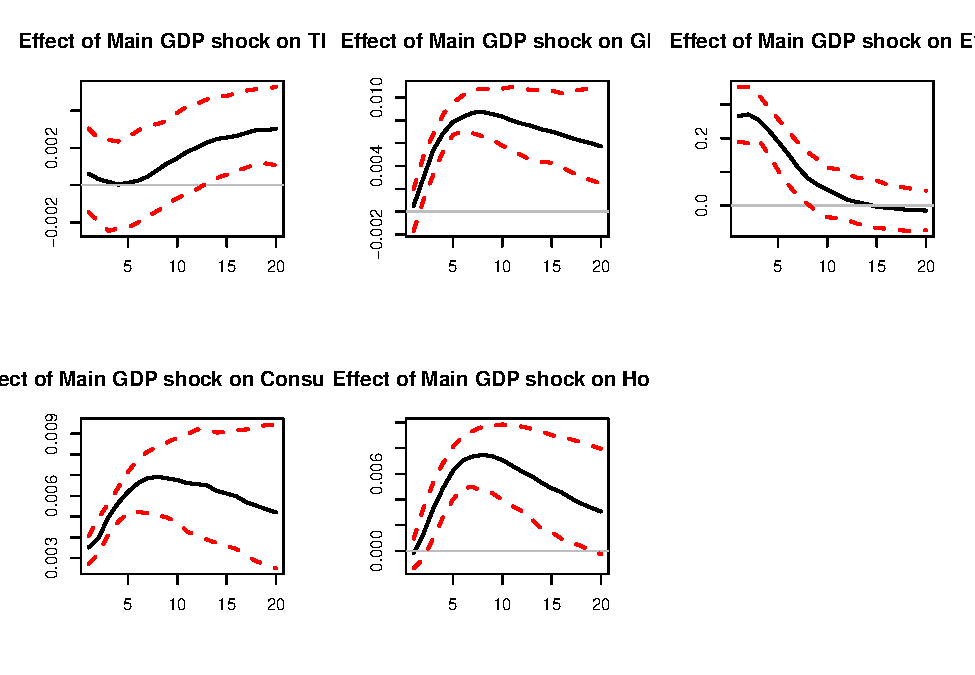
\includegraphics[width=0.95\linewidth]{IdentifStructShocks_files/figure-latex/uhlig-1} \caption{Main GDP shock.}\label{fig:uhlig}
\end{figure}

The ``main GDP shock'\,' explains 82\% of the variance of GDP at horizon 20.

\citet{BARSKY2011273} exploit this approach to identify a ``TFP news shock'', that they define as the shock (a) that is orthogonal to the innovation in current utilization-adjusted TFP and (b) that best explains variation in future TFP. \citet{Levchenko_Pandalai-Nayar_2018} add a ``sentiment shock'' that they define as the shock (a) that is orthogonal to both the innovation in current utilization-adjusted TFP and to the TFP news shock, and (b) that best explains variation in consumer sentiment. The following code replicates \citet{Levchenko_Pandalai-Nayar_2018}. They use a mix of zero and FEVD to identify TFP surprises, TFP news, and sentiment shocks. We adopt a different approach by using FEVD to capture zero restrictions.

\begin{Shaded}
\begin{Highlighting}[]
\NormalTok{names.of.shocks }\OtherTok{\textless{}{-}} \FunctionTok{c}\NormalTok{(}\StringTok{"TFP surprise"}\NormalTok{,}\StringTok{"TFP news"}\NormalTok{,}\StringTok{"Sentiment"}\NormalTok{)}
\CommentTok{\#define horizons for FEVM}
\NormalTok{H1 }\OtherTok{\textless{}{-}} \FunctionTok{array}\NormalTok{(}\DecValTok{0}\NormalTok{,}\FunctionTok{c}\NormalTok{(}\DecValTok{1}\NormalTok{,}\DecValTok{3}\NormalTok{))}
\NormalTok{H2 }\OtherTok{\textless{}{-}} \FunctionTok{array}\NormalTok{(}\DecValTok{0}\NormalTok{,}\FunctionTok{c}\NormalTok{(}\DecValTok{1}\NormalTok{,}\DecValTok{3}\NormalTok{))}
\NormalTok{H1[}\DecValTok{1}\NormalTok{,}\DecValTok{1}\NormalTok{] }\OtherTok{\textless{}{-}} \DecValTok{1}
\NormalTok{H1[}\DecValTok{1}\NormalTok{,}\DecValTok{2}\NormalTok{] }\OtherTok{\textless{}{-}} \DecValTok{1}
\NormalTok{H1[}\DecValTok{1}\NormalTok{,}\DecValTok{3}\NormalTok{] }\OtherTok{\textless{}{-}} \DecValTok{1}
\NormalTok{H2[}\DecValTok{1}\NormalTok{,}\DecValTok{1}\NormalTok{] }\OtherTok{\textless{}{-}} \DecValTok{1}
\NormalTok{H2[}\DecValTok{1}\NormalTok{,}\DecValTok{2}\NormalTok{] }\OtherTok{\textless{}{-}} \DecValTok{40}
\NormalTok{H2[}\DecValTok{1}\NormalTok{,}\DecValTok{3}\NormalTok{] }\OtherTok{\textless{}{-}} \DecValTok{2}
\NormalTok{variable }\OtherTok{\textless{}{-}} \FunctionTok{c}\NormalTok{(}\DecValTok{1}\NormalTok{,}\DecValTok{1}\NormalTok{,}\DecValTok{3}\NormalTok{) }\CommentTok{\# variables for which we want to maximize FEVD}
\NormalTok{norm }\OtherTok{\textless{}{-}} \FunctionTok{c}\NormalTok{(}\DecValTok{1}\NormalTok{,}\DecValTok{20}\NormalTok{,}\DecValTok{2}\NormalTok{) }\CommentTok{\# horizon at which the impact of the}
\CommentTok{\# shock is normalized to be positive}
\NormalTok{res.svar.fevmax }\OtherTok{\textless{}{-}}
  \FunctionTok{svar.fevmax}\NormalTok{(y,}\AttributeTok{p=}\DecValTok{2}\NormalTok{,}
              \AttributeTok{nb.shocks=}\DecValTok{3}\NormalTok{,}
\NormalTok{              names.of.shocks,}
\NormalTok{              H1,}
\NormalTok{              H2,}
\NormalTok{              variable,}
\NormalTok{              norm,}
              \AttributeTok{nb.periods.IRF =} \DecValTok{40}\NormalTok{,}
              \AttributeTok{bootstrap.replications =} \DecValTok{100}\NormalTok{, }\CommentTok{\# This is used in the}
              \CommentTok{\#parametric bootstrap only}
              \AttributeTok{confidence.interval =} \FloatTok{0.90}\NormalTok{, }\CommentTok{\# expressed in pp.}
              \AttributeTok{indic.plot =} \DecValTok{1} \CommentTok{\# Plots are displayed if = 1.}
\NormalTok{  )}
\end{Highlighting}
\end{Shaded}

\begin{figure}
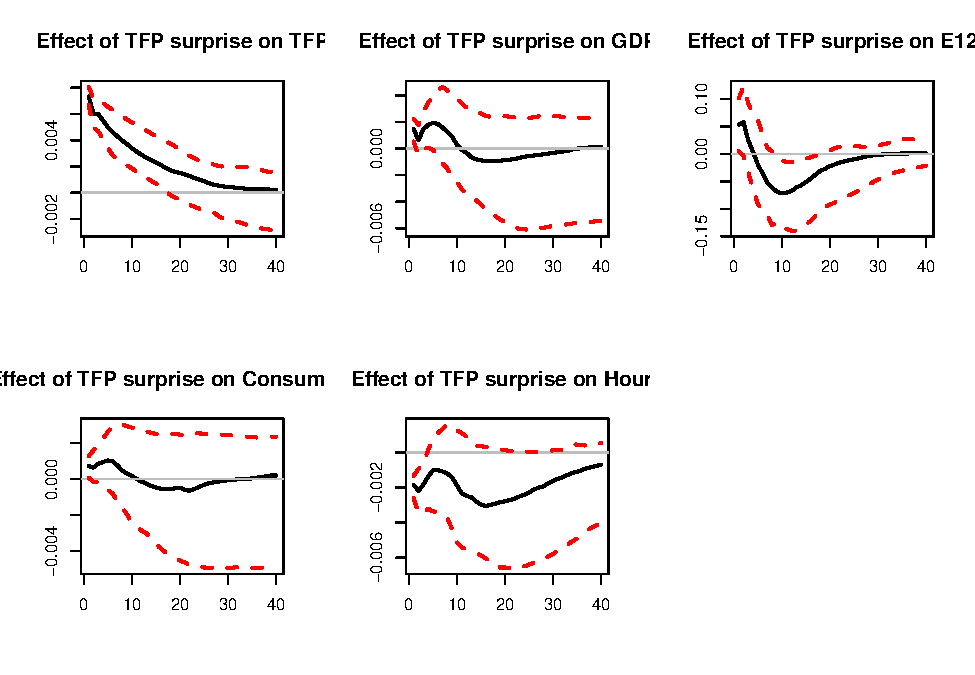
\includegraphics[width=0.95\linewidth]{IdentifStructShocks_files/figure-latex/levchenko-1} \caption{Replication of Levchenko and Pandalai-Nayar (2020). FEVD and zero restrictions.}\label{fig:levchenko-1}
\end{figure}
\begin{figure}
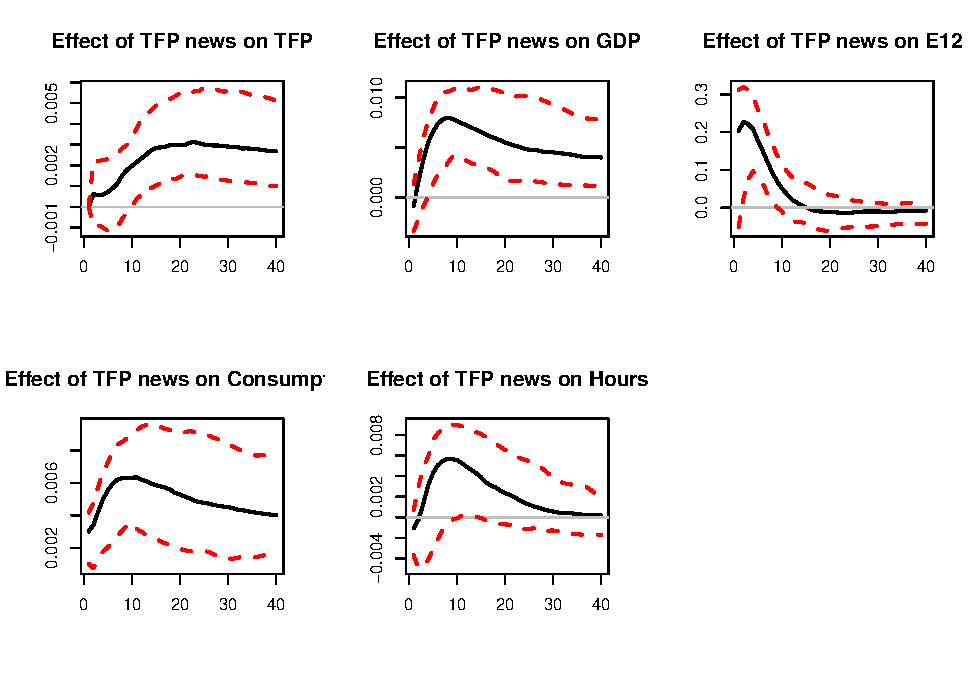
\includegraphics[width=0.95\linewidth]{IdentifStructShocks_files/figure-latex/levchenko-2} \caption{Replication of Levchenko and Pandalai-Nayar (2020). FEVD and zero restrictions.}\label{fig:levchenko-2}
\end{figure}

\begin{Shaded}
\begin{Highlighting}[]
\NormalTok{Variance.decomp }\OtherTok{\textless{}{-}} \FunctionTok{variance.decomp}\NormalTok{(res.svar.fevmax}\SpecialCharTok{$}\NormalTok{simulated.IRFs)}
\NormalTok{vardecomp }\OtherTok{\textless{}{-}}\NormalTok{ Variance.decomp}\SpecialCharTok{$}\NormalTok{vardecomp}
\FunctionTok{mean}\NormalTok{(vardecomp[}\DecValTok{2}\NormalTok{,}\DecValTok{2}\NormalTok{,}\DecValTok{40}\NormalTok{,,}\DecValTok{3}\NormalTok{])}\CommentTok{\# mean contribution (across all simulated IRFs)}
\end{Highlighting}
\end{Shaded}

\begin{verbatim}
## [1] 0.1115537
\end{verbatim}

\begin{Shaded}
\begin{Highlighting}[]
\CommentTok{\# of 3rd shock to variance of second variable, horizon 40.}
\end{Highlighting}
\end{Shaded}

\begin{figure}
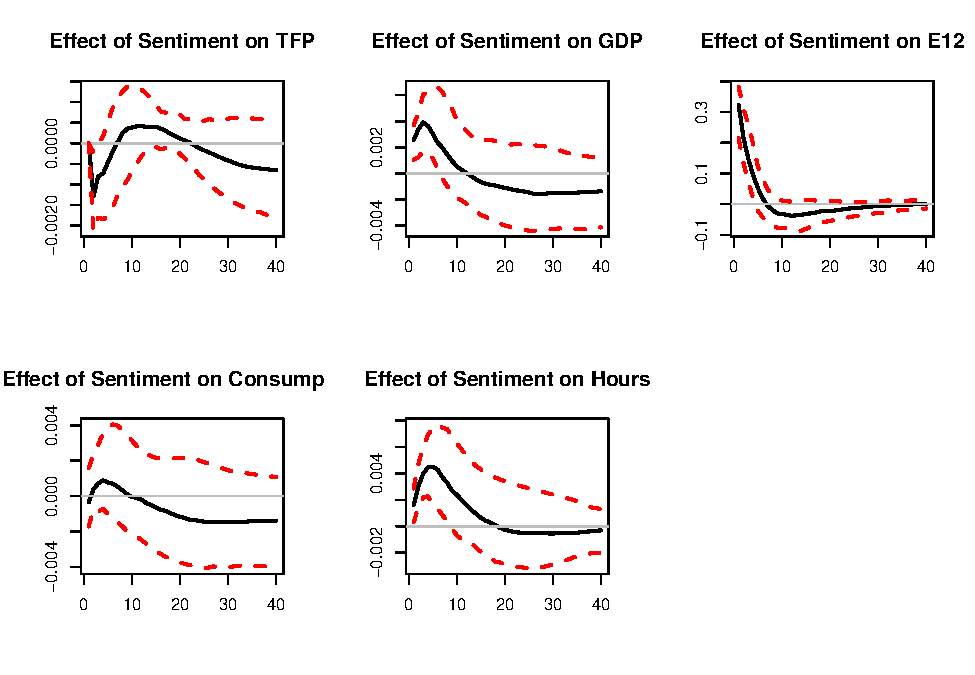
\includegraphics[width=0.95\linewidth]{IdentifStructShocks_files/figure-latex/levchenko-3} \caption{Replication of Levchenko and Pandalai-Nayar (2020). FEVD and zero restrictions.}\label{fig:levchenko-3}
\end{figure}

Sentiment shocks explain 11\% of the variance of GDP, against 75\% for TFP shocks (including 64\% for TFP news shocks).

\section{Restrictions based on narrative historical decomposition}\label{NarrativeHistDecomp}

A related approach, introduced by \citet{AntolinDiaz_RubioRamirez_2018}, consists in imposing that, on some specific dates (based on narrative information), a particular shock was the most important contributor to the unexpected movement of some variable during a particular period.\footnote{See also Section \ref{NarrativeSign}.} This can be formalized in two different ways (respectively called Type A and Type B by \citet{AntolinDiaz_RubioRamirez_2018}):

\begin{itemize}
\tightlist
\item
  Type A: A given shock is the most important (least important) driver of the unexpected change in a variable during some periods. For these periods, the absolute value of its contribution to the unexpected change in a variable is larger (smaller) than the absolute value of the contribution of any other structural shock.
\item
  Type B: A given shock is the overwhelming (negligible) driver of the unexpected change in a given variable during the period. For these periods, the absolute value of its contribution to the unexpected change in a variable is larger (smaller) than the sum of the absolute value of the contributions of all other structural shocks.
\end{itemize}

\chapter{Identification based on non-normality of the shocks}\label{NonGaussian}

\section{Intuition}\label{intuition}

In this section, we show that the non-identification of the structural shocks (\(\eta_t\)) is specific to the Gaussian case. We propose consistent estimation approaches for SVAR in the context of non-Gaussian shocks.

We have seen in what precedes that we cannot identify \(B\) based on first and second moments only. Since a Gaussian distribution is perfectly determined by the first two moments, it comes that one cannot achieve identification when the structural shocks are Gaussian. That is, even if we observe an infinite number of i.i.d. \(B \eta_t\), we cannot recover \(B\) is the \(\eta_t\)'s are Gaussian.

Indeed, if \(\eta_t \sim \mathcal{N}(0,Id)\), then the distribution of \(\varepsilon_t \equiv B \eta_t\) is \(\mathcal{N}(0,BB')\). Hence \(\Omega = B B'\) is observed (in the population), but for any orthogonal matrix \(Q\) (i.e.~\(QQ'=Id\)), we also have \(BQ \eta_t \sim \mathcal{N}(0,\Omega)\).

To illustrate, consider the following bivariate Gaussian situations, with \(\Theta_1=0\)):

\(\left[\begin{array}{c}\eta_{1,t}\\ \eta_{2,t}\end{array}\right]\sim \mathcal{N}(0,Id)\), with
\(B = \left[\begin{array}{cc}
1 & 2 \\
-1 & 1
\end{array}\right]\) and
\(Q = \left[\begin{array}{cc}
\cos(\pi/3) & -\sin(\pi/3) \\
\sin(\pi/3) & \cos(\pi/3)
\end{array}\right]\) (rotation).

Figure \ref{fig:preMadeFigureICA} shows that the distributions of \(B \eta_t\) and of \(BQ\eta_t\) are identical. However, the impulse response functions associated with one of the other impulse matrix (\(B\) or \(BQ\)) are different. This is illustrated by Figure \ref{fig:preMadeFigureICA2}, that shows the IRFs associated with two identical models (defined by Eq. \eqref{eq:VARMA111}), the only difference being the impulse matrix (\(B\) or \(BQ\)).

\begin{figure}
\includegraphics[width=0.95\linewidth]{images/Figure_A} \caption{This figure compares the distributions of two Gaussian bivariate vectors, $B \eta_t$ and $BQ\eta_t$, where $\eta_{t} \sim \mathcal{N}(0,Id)$ (therefore $\eta_{1,t}$ and $\eta_{2,t}$ are independent), and $Q$  is an orthogonal matrix.}\label{fig:preMadeFigureICA}
\end{figure}

\begin{figure}
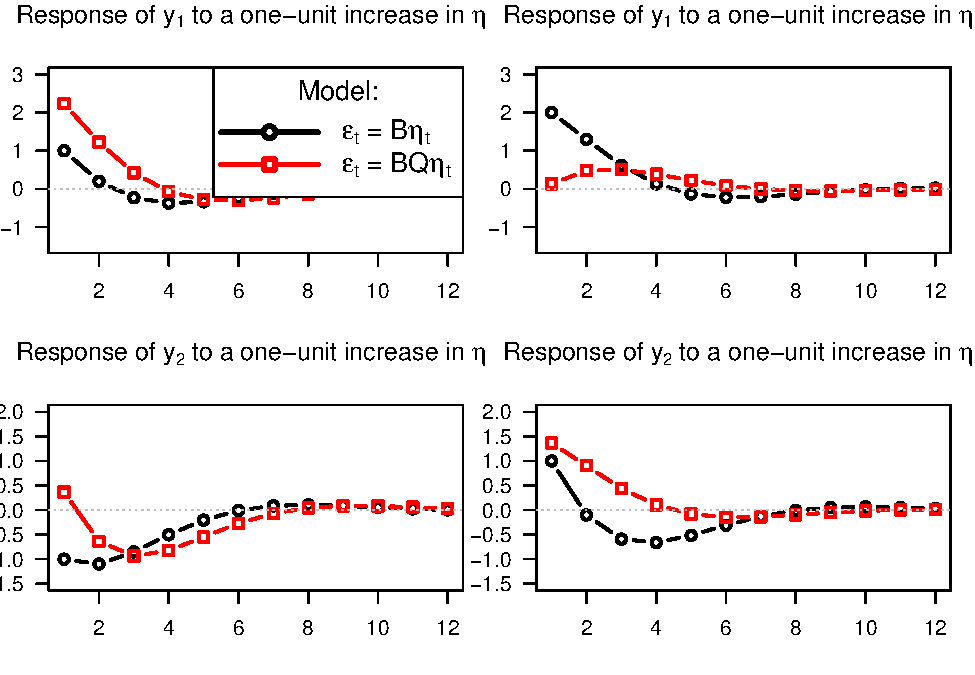
\includegraphics[width=0.95\linewidth]{IdentifStructShocks_files/figure-latex/preMadeFigureICA2-1} \caption{This figure shows that the impulse response functions associated with an impulse matrix equal to $B$ (black line) or $BQ$ (red line) are different (even if $BB'=BQ(BQ)'$).}\label{fig:preMadeFigureICA2}
\end{figure}

Hence, in the Gaussian case, external restrictions (economic hypotheses) are needed to identify \(B\) (see previous sections). But such restrictions may not be necessary if the structural shocks are not Gaussian. That is, the identification problem is very specific to normally-distributed \(\eta_t\)'s (\citet{Rigobon_2003}, \citet{NORMANDIN20041217}, \citet{Lanne_Lutkepohl_2008}).

To better see why this can be the case, consider again a bivariate vector of independent structural shocks (\(\eta_{1,t}\) and \(\eta_{2,t}\)) but, now, assume that one of them is not Gaussian any more. Specifically, assume that \(\eta_{2,t}\) is drawn from a Student distribution with 5 degrees of freedom:
\(\eta_{1,t} \sim \mathcal{N}(0,1)\), \(\eta_{2,t} \sim t(5)\),
\(B = \left[\begin{array}{cc}
1 & 2 \\
-1 & 1
\end{array}\right]\) and
\(Q = \left[\begin{array}{cc}
\cos(\pi/3) & -\sin(\pi/3) \\
\sin(\pi/3) & \cos(\pi/3)
\end{array}\right]\).

Figure \ref{fig:preMadeFigureICAGaussianStudent} shows that, in this case, \(B \eta_t\) and \(BQ\eta_t\) do not have the same distribution any more (in spite of the fact that, in both cases, we have \(\mathbb{V}ar(\varepsilon_t)=BB'\)). This opens the door to the identification of the impulse matrix (\(BQ\)) in the non-Gaussian case.

\begin{figure}
\includegraphics[width=0.95\linewidth]{images/Figure_C} \caption{This figure compares the distributions of two Gaussian bivariate vectors, $B \eta_t$ and $BQ\eta_t$, where $\eta_t{1,t} \sim \mathcal{N}(0,1)$, $\eta_t{2,t} \sim t(5)$, and $Q$  is an orthogonal matrix.}\label{fig:preMadeFigureICAGaussianStudent}
\end{figure}

\section{Independent Component Analysis (ICA)}\label{independent-component-analysis-ica}

The exercise that consists in identifying non-Gaussian independent shocks out of linear combinations of these shocks is a well-known problem of the signal-processing literature, called \textbf{independent component analysis (ICA)}. Let us denote by \(C\) the matrix that is such that \(C = \Omega^{-1/2}B\), where \(\Omega^{1/2}\) results from the Cholesky decomposition of \(\Omega = BB'\) (implying, \(\Omega^{1/2}{\Omega^{1/2}}'=\Omega\)). It is easy to check that \(C\) is an orthogonal matrix (and we have \(B = \Omega^{1/2}C\)).

The classical ICA problem is as follows: Find \(C\) such that \(\varepsilon_t = C \eta_t\) (or \(\eta_t = C'\varepsilon_t\)) given that:\footnote{The \(\varepsilon_t\)'s that we consider here are \emph{standardized} VAR residuals, obtained by pre-multiplying the actual VAR residuals by \(\Omega^{-1/2}\).}

\begin{enumerate}
\def\labelenumi{\roman{enumi}.}
\tightlist
\item
  We observe the \(\varepsilon_t\)'s,
\item
  The components of \(\eta_t\) are independent,
\item
  \(CC'=Id\) (i.e., \(C\) is orthogonal).
\end{enumerate}

Figure \ref{fig:ThreePlots} represents again some bivariate distributions. The black (red) lines correspond to the distributions of \(\eta_t\) (\(C\eta_t\)). It is important to note that the two components of vector \(C \eta_t\) are not independent (contrary to those of \(\eta_t\)).

\begin{figure}

\includegraphics[width=0.95\linewidth]{images/Figure_E} \hfill{}

\caption{The three plots represent the bivariate distributions of $\eta_t$ (black) and of $C\eta_t$ (red), where the two components of $\eta_t$ are independent, of unit variance, and $C$ is orthogonal. Hence, for each of the three plots, $\mathbb{V}ar(C\eta_t)=Id$.}\label{fig:ThreePlots}
\end{figure}

In all cases, we have \(\mathbb{V}ar(\varepsilon_t)=\mathbb{V}ar(\eta_t)=Id\). But the two components of \(\varepsilon_t\) are not independent. For instance, in the last two cases, we have \(\mathbb{E}(\varepsilon_{2,t}|\varepsilon_{1,t}>4)<0\) (whereas \(\mathbb{E}(\eta_{2,t}|\eta_{1,t}>4)=0\)). The objective of ICA is to rotate \(\varepsilon_t\) to retrieve independent components (\(\eta_t\)).

\begin{hypothesis}
\protect\hypertarget{hyp:NonGauss}{}\label{hyp:NonGauss}

Process \(\eta_t\) satisfies:

\begin{enumerate}
\def\labelenumi{\roman{enumi}.}
\tightlist
\item
  The \(\eta_t\)'s are i.i.d. (across time) with \(\mathbb{E}(\eta_t) = 0\) and \(\mathbb{V}ar(\eta_t) = Id.\)
\item
  The components \(\eta_{1,t}, \ldots, \eta_{n,t}\) are mutually independent.
  iii We have
  \[
  \varepsilon_t = C_0 \eta_t,
  \]
  with \(\mathbb{V}ar(\varepsilon_t) = Id\) (i.e., \(C_0\) is orthogonal).
\end{enumerate}

\end{hypothesis}

\begin{theorem}[Eriksson, Koivunen (2004)]
\protect\hypertarget{thm:EK2004}{}\label{thm:EK2004}If Hypothesis \ref{hyp:NonGauss} is satisfied and if at most one of the components of \(\eta\) is Gaussian, then matrix \(C_0\) is identifiable up to the post multiplication by \(DP\), where \(P\) is a permutation matrix and \(D\) is a diagonal matrix whose diagonal entries are 1 or \(-1\).\}
\end{theorem}

\section{Pseudo-Maximum Likelihood (PML) approach}\label{pseudo-maximum-likelihood-pml-approach}

Hence, non-normal structural shocks are identifiable. But how to estimate them based on observations of the \(\varepsilon_t\)'s? \citet{Gourieroux_Monfort_Renne_2017} have proposed a \textbf{Pseudo-Maximum Likelihood (PML)} approach. This approach consists in maximizing a so-called \textbf{pseudo log-likelihood function}, based on a set of p.d.f. \(g_i (\eta_i), i=1,\ldots,n\) (that may be different from the true p.d.f. of the \(\eta_{i,t}\)'s):
\begin{equation}
\log \mathcal{L}_T (C) = \sum^T_{t=1} \sum^n_{i=1} \log g_i (c'_i \varepsilon_t),\label{eq:pseudolog}
\end{equation}
where \(c_i\) is the \(i^{th}\) column of matrix \(C\) (or \(c'_i\) is the \(i^{th}\) row of \(C^{-1}\) since \(C^{-1}=C'\)).

The log-likelihood function \eqref{eq:pseudolog} is computed as if the errors \(\eta_{i,t}\) had the pdf \(g_i (\eta_i)\). The PML estimator of matrix \(C\) maximizes the pseudo log-likelihood function:
\begin{equation}
\widehat{C_T} = \arg \max_C \sum^T_{t=1} \sum^n_{i=1} \log g_i (c'_i \varepsilon_t),\label{eq:optimprob}
\end{equation}

\centerline{$s.t. \;C'C = Id.$}

The restrictions \(C'C = Id\) can be eliminated by parameterizing \(C\) in such a way that, whatever the considered parameters, \(C\) is orthogonal.\footnote{\citet{Jarocinski_2021} develops a ML approach that does not necessitates to parameterize the space of orthogonal matrices as he does not proceed under the assumption that \(C'C\) is orthogonal.} \citet{Gourieroux_Monfort_Renne_2017} propose to use, for that, the Cayley's representation: any orthogonal matrix with no eigenvalue equal to \(-1\) can be written as
\begin{equation}
C(A) = (Id+A) (Id-A)^{-1},
\end{equation}
where \(A\) is a skew symmetric (or antisymmetric) matrix, such that \(A'=-A\). There is a one-to-one relationship with \(A\), since:
\begin{equation}
A = (C(A)+Id)^{-1} (C(A)-Id).
\end{equation}

Hence, the PML estimator of matrix \(C\) is obtained as \(\widehat{C_T} = C(\hat{A}_T),\) where:
\begin{equation}
\hat{A}_T = \arg \max_{a_{i,j}, i>j} \sum^T_{t=1} \sum^n_{i=1} \log g_i [c_i (A)' \varepsilon_t].\label{eq:optimprob2}
\end{equation}

Under assumptions on the \(g_i\) functions (excluding the Gaussian distributions), \citet{Gourieroux_Monfort_Renne_2017} derive the asymptotic properties of the PML estimator. Specifically, the PML estimator \(\widehat{C_T}\) of \(C_0\) is consistent (in \(\mathcal{P}_0\), the set of matrices obtained by permutation and sign change of the columns of \(C_0\)) and asymptotically normal, with speed of convergence \(1/\sqrt{T}\).

The asymptotic variance-covariance matrix of \(vec \sqrt{T} (\widehat{C_T} - C_0)\) is \(A^{-1} \left[\begin{array}{cc} \Gamma & 0 \\ 0 & 0 \end{array} \right] (A')^{-1}\), where matrices \(A\) and \(\Gamma\) are detailed in \citet{Gourieroux_Monfort_Renne_2017}.

Note that the potential misspecification of pseudo-distributions \(g_i\) has no effect on the consistency of these specific PML estimators.

Table \ref{tab:distriICA} reports usual p.d.f. and their derivatives. (The latter are needed to compute the asymptotic variance-covariance matrix of \(vec \sqrt{T} (\widehat{C_T} - C_0)\).)

\begin{longtable}[]{@{}
  >{\raggedright\arraybackslash}p{(\linewidth - 6\tabcolsep) * \real{0.0851}}
  >{\raggedright\arraybackslash}p{(\linewidth - 6\tabcolsep) * \real{0.3106}}
  >{\raggedright\arraybackslash}p{(\linewidth - 6\tabcolsep) * \real{0.2511}}
  >{\raggedright\arraybackslash}p{(\linewidth - 6\tabcolsep) * \real{0.3532}}@{}}
\caption{\label{tab:distriICA} This table reports usual p.d.f. and their derivatives.}\tabularnewline
\toprule\noalign{}
\begin{minipage}[b]{\linewidth}\raggedright
\end{minipage} & \begin{minipage}[b]{\linewidth}\raggedright
\(\log g(x)\)
\end{minipage} & \begin{minipage}[b]{\linewidth}\raggedright
\(\dfrac{d \log g(x)}{d x}\)
\end{minipage} & \begin{minipage}[b]{\linewidth}\raggedright
\(\dfrac{d^2 \log g(x)}{d x^2}\)
\end{minipage} \\
\midrule\noalign{}
\endfirsthead
\toprule\noalign{}
\begin{minipage}[b]{\linewidth}\raggedright
\end{minipage} & \begin{minipage}[b]{\linewidth}\raggedright
\(\log g(x)\)
\end{minipage} & \begin{minipage}[b]{\linewidth}\raggedright
\(\dfrac{d \log g(x)}{d x}\)
\end{minipage} & \begin{minipage}[b]{\linewidth}\raggedright
\(\dfrac{d^2 \log g(x)}{d x^2}\)
\end{minipage} \\
\midrule\noalign{}
\endhead
\bottomrule\noalign{}
\endlastfoot
Gaussian & \(cst - x^2/2\) & \(-x\) & \(-1\) \\
Student \(t(\nu>4)\) & \(-\dfrac{1-\nu}{2}\log\left( 1 +\dfrac{x^2}{\nu-2} \right)\) & \(-\dfrac{x(1+\nu)}{\nu - 2 + x^2}\) & \(- (1+\nu)  \dfrac{\nu - 2 - x^2}{\nu - 2 + x^2}\) \\
Hyperbolic secant & \(cst - \log\left( \cosh\left\{\dfrac{\pi}{2}x\right\} \right)\) & \(-\dfrac{\pi}{2}   anh\left(\dfrac{\pi}{2}x\right)\) & \(-\left(\dfrac{\pi}{2}\dfrac{1}{\cosh\left(\dfrac{\pi}{2}x\right)}\right)^2\) \\
Subgaussian & \(cst + \pi x^2 + \log \left(\cosh\left\{\dfrac{\pi}{2}x\right\}\right)\) & \(2\pi x+\dfrac{\pi}{2}\tanh\left(x \dfrac{\pi}{2}\right)\) & \(2\pi +\left(\dfrac{\pi}{2}\dfrac{1}{\cosh\left(\dfrac{\pi}{2}x\right)}\right)^2\) \\
\end{longtable}

\begin{example}[Non-Gaussian monetary-policy shocks]
\protect\hypertarget{exm:GMR2017}{}\label{exm:GMR2017}We apply the PML-ICA approach on U.S. data coerving the period 1959:IV to 2015:I at the quarterly frequency (\(T=224\)). We consider three dependent variables: inflation (\(\pi_t\)), economic activity (\(z_t\), the output gap) and the nominal short-term interest rate (\(r_t\)). Changes in the log of oil prices are added as an exogenous variable (\(x_t\)).

\begin{Shaded}
\begin{Highlighting}[]
\FunctionTok{library}\NormalTok{(IdSS)}
\NormalTok{First.date }\OtherTok{\textless{}{-}} \StringTok{"1959{-}04{-}01"}
\NormalTok{Last.date  }\OtherTok{\textless{}{-}} \StringTok{"2015{-}01{-}01"}
\NormalTok{data }\OtherTok{\textless{}{-}}\NormalTok{ US3var}
\NormalTok{data }\OtherTok{\textless{}{-}}\NormalTok{ data[(data}\SpecialCharTok{$}\NormalTok{Date}\SpecialCharTok{\textgreater{}=}\NormalTok{First.date)}\SpecialCharTok{\&}\NormalTok{(data}\SpecialCharTok{$}\NormalTok{Date}\SpecialCharTok{\textless{}=}\NormalTok{Last.date),]}
\NormalTok{Y }\OtherTok{\textless{}{-}} \FunctionTok{as.matrix}\NormalTok{(data[}\FunctionTok{c}\NormalTok{(}\StringTok{"infl"}\NormalTok{,}\StringTok{"y.gdp.gap"}\NormalTok{,}\StringTok{"r"}\NormalTok{)])}
\NormalTok{names.var }\OtherTok{\textless{}{-}} \FunctionTok{c}\NormalTok{(}\StringTok{"inflation"}\NormalTok{,}\StringTok{"real activity"}\NormalTok{,}\StringTok{"short{-}term rate"}\NormalTok{)}
\NormalTok{T }\OtherTok{\textless{}{-}} \FunctionTok{dim}\NormalTok{(Y)[}\DecValTok{1}\NormalTok{]}
\NormalTok{n }\OtherTok{\textless{}{-}} \FunctionTok{dim}\NormalTok{(Y)[}\DecValTok{2}\NormalTok{]}
\end{Highlighting}
\end{Shaded}

Let us denote by \(W_t\) the set of information made of the past values of \(y_t= [\pi_t,z_t,r_t]\), that is \(\{y_{t-1},y_{t-2},\dots\}\), and of exogenous variables \(\{x_{t},x_{t-1},\dots\}\). The reduced-form VAR model reads:
\[
y_t  = \underbrace{\mu + \sum_{i=1}^{p} \Phi_i y_{t-i} + \Theta x_t}_{a(W_t;\theta)} + u_t
\]
where the \(u_t\)'s are assumed to be serially independent, with zero mean and variance-covariance matrix \(\Omega\).

Matrices \(\mu\), \(\Phi_i\), \(\Theta\) and \(\Omega\) are consistently estimated by OLS. Jarque-Bera tests support the hypothesis of non-normality for all residuals.

\begin{Shaded}
\begin{Highlighting}[]
\NormalTok{nb.lags }\OtherTok{\textless{}{-}} \DecValTok{6} \CommentTok{\# number of lags used in the VAR model}
\NormalTok{X }\OtherTok{\textless{}{-}} \ConstantTok{NULL}
\ControlFlowTok{for}\NormalTok{(i }\ControlFlowTok{in} \DecValTok{1}\SpecialCharTok{:}\NormalTok{nb.lags)\{}
\NormalTok{  lagged.Y }\OtherTok{\textless{}{-}} \FunctionTok{rbind}\NormalTok{(}\FunctionTok{matrix}\NormalTok{(}\ConstantTok{NaN}\NormalTok{,i,n),Y[}\DecValTok{1}\SpecialCharTok{:}\NormalTok{(T}\SpecialCharTok{{-}}\NormalTok{i),])}
\NormalTok{  X }\OtherTok{\textless{}{-}} \FunctionTok{cbind}\NormalTok{(X,lagged.Y)\}}
\NormalTok{X }\OtherTok{\textless{}{-}} \FunctionTok{cbind}\NormalTok{(X,data}\SpecialCharTok{$}\NormalTok{commo) }\CommentTok{\# add exogenous variables}
\NormalTok{Phi }\OtherTok{\textless{}{-}} \FunctionTok{matrix}\NormalTok{(}\DecValTok{0}\NormalTok{,n,n}\SpecialCharTok{*}\NormalTok{nb.lags);mu }\OtherTok{\textless{}{-}} \FunctionTok{rep}\NormalTok{(}\DecValTok{0}\NormalTok{,n)}
\NormalTok{effect.commo }\OtherTok{\textless{}{-}} \FunctionTok{rep}\NormalTok{(}\DecValTok{0}\NormalTok{,n)}
\NormalTok{U }\OtherTok{\textless{}{-}} \ConstantTok{NULL} \CommentTok{\# Eta is the matrix of OLS residuals}
\ControlFlowTok{for}\NormalTok{(i }\ControlFlowTok{in} \DecValTok{1}\SpecialCharTok{:}\NormalTok{n)\{}
\NormalTok{  eq }\OtherTok{\textless{}{-}} \FunctionTok{lm}\NormalTok{(Y[,i] }\SpecialCharTok{\textasciitilde{}}\NormalTok{ X)}
\NormalTok{  Phi[i,] }\OtherTok{\textless{}{-}}\NormalTok{ eq}\SpecialCharTok{$}\NormalTok{coef[}\DecValTok{2}\SpecialCharTok{:}\NormalTok{(}\FunctionTok{dim}\NormalTok{(Phi)[}\DecValTok{2}\NormalTok{]}\SpecialCharTok{+}\DecValTok{1}\NormalTok{)]}
\NormalTok{  mu[i] }\OtherTok{\textless{}{-}}\NormalTok{ eq}\SpecialCharTok{$}\NormalTok{coef[}\DecValTok{1}\NormalTok{]}
\NormalTok{  U }\OtherTok{\textless{}{-}} \FunctionTok{cbind}\NormalTok{(U,eq}\SpecialCharTok{$}\NormalTok{residuals)}
\NormalTok{  effect.commo[i] }\OtherTok{\textless{}{-}}\NormalTok{ eq}\SpecialCharTok{$}\NormalTok{coef[}\FunctionTok{length}\NormalTok{(eq}\SpecialCharTok{$}\NormalTok{coef)]}
\NormalTok{\}}
\NormalTok{Omega }\OtherTok{\textless{}{-}} \FunctionTok{var}\NormalTok{(U) }\CommentTok{\# Covariance matrix of the OLS residuals.}
\NormalTok{Omeg12 }\OtherTok{\textless{}{-}} \FunctionTok{t}\NormalTok{(}\FunctionTok{chol}\NormalTok{(Omega)) }\CommentTok{\# Cholesky matrix associated with Omega (lower triang.)}
\NormalTok{Eps }\OtherTok{\textless{}{-}}\NormalTok{ U }\SpecialCharTok{\%*\%} \FunctionTok{t}\NormalTok{(}\FunctionTok{solve}\NormalTok{(Omeg12)) }\CommentTok{\# Recover associated structural shocks}
\end{Highlighting}
\end{Shaded}

We want to estimate the orthogonal matrix \(C\) such that \(u_t=\Omega^{1/2}C \eta_t\), where

\begin{itemize}
\tightlist
\item
  \(\Omega^{1/2}\) results from the Cholesky decomposition of \(\Omega\) and
\item
  the components of \(\eta_t\) are independent, zero-mean with unit variance.
\end{itemize}

The PML approach is applied on standardized VAR residuals given by:
\[
\hat\varepsilon_t = \hat\Omega^{-1/2}_T\underbrace{[y_t - a(W_t;\hat\theta_T)]}_{\mbox{VAR residuals}}.
\]
By construction of \(\hat\Omega^{-1/2}_T\), it comes that the covariance matrix of these residuals is \(Id\).

The pseudo density functions are distinct and asymmetric mixtures of Gaussian distributions.

\begin{Shaded}
\begin{Highlighting}[]
\NormalTok{distri }\OtherTok{\textless{}{-}} \FunctionTok{list}\NormalTok{(}
  \AttributeTok{type=}\FunctionTok{c}\NormalTok{(}\StringTok{"mixt.gaussian"}\NormalTok{,}\StringTok{"mixt.gaussian"}\NormalTok{,}\StringTok{"mixt.gaussian"}\NormalTok{),}
  \AttributeTok{df=}\FunctionTok{c}\NormalTok{(}\ConstantTok{NaN}\NormalTok{,}\ConstantTok{NaN}\NormalTok{,}\ConstantTok{NaN}\NormalTok{),}
  \AttributeTok{p=}\FunctionTok{c}\NormalTok{(}\FloatTok{0.5}\NormalTok{,.}\DecValTok{5}\NormalTok{,.}\DecValTok{5}\NormalTok{),}\AttributeTok{mu=}\FunctionTok{c}\NormalTok{(.}\DecValTok{1}\NormalTok{,.}\DecValTok{1}\NormalTok{,.}\DecValTok{1}\NormalTok{),}\AttributeTok{sigma=}\FunctionTok{c}\NormalTok{(.}\DecValTok{5}\NormalTok{,.}\DecValTok{7}\NormalTok{,}\FloatTok{1.3}\NormalTok{))}
\NormalTok{AA}\FloatTok{.0} \OtherTok{\textless{}{-}} \FunctionTok{c}\NormalTok{(}\DecValTok{0}\NormalTok{,}\DecValTok{0}\NormalTok{,}\DecValTok{0}\NormalTok{)}
\NormalTok{res.optim }\OtherTok{\textless{}{-}} \FunctionTok{optim}\NormalTok{(AA}\FloatTok{.0}\NormalTok{,func.}\FloatTok{2.}\NormalTok{minimize,}
                   \AttributeTok{Y =}\NormalTok{ Eps, }\AttributeTok{distri =}\NormalTok{ distri,}
                   \AttributeTok{gr =}\NormalTok{ d.func.}\FloatTok{2.}\NormalTok{minimize,}
                   \AttributeTok{method=}\StringTok{"Nelder{-}Mead"}\NormalTok{,}
                   \AttributeTok{control=}\FunctionTok{list}\NormalTok{(}\AttributeTok{trace=}\ConstantTok{FALSE}\NormalTok{,}\AttributeTok{maxit=}\DecValTok{1000}\NormalTok{))}
\NormalTok{AA}\FloatTok{.0} \OtherTok{\textless{}{-}}\NormalTok{ res.optim}\SpecialCharTok{$}\NormalTok{par}
\NormalTok{res.optim }\OtherTok{\textless{}{-}} \FunctionTok{optim}\NormalTok{(AA}\FloatTok{.0}\NormalTok{,func.}\FloatTok{2.}\NormalTok{minimize,d.func.}\FloatTok{2.}\NormalTok{minimize,}
                   \AttributeTok{Y =}\NormalTok{ Eps, }\AttributeTok{distri =}\NormalTok{ distri,}
                   \AttributeTok{method=}\StringTok{"BFGS"}\NormalTok{,}
                   \AttributeTok{control=}\FunctionTok{list}\NormalTok{(}\AttributeTok{trace=}\ConstantTok{FALSE}\NormalTok{))}
\NormalTok{AA.est }\OtherTok{\textless{}{-}}\NormalTok{ res.optim}\SpecialCharTok{$}\NormalTok{par}
\NormalTok{n }\OtherTok{\textless{}{-}} \FunctionTok{ncol}\NormalTok{(Y)}
\NormalTok{M }\OtherTok{\textless{}{-}} \FunctionTok{make.M}\NormalTok{(n)}
\NormalTok{A.est }\OtherTok{\textless{}{-}} \FunctionTok{matrix}\NormalTok{(M }\SpecialCharTok{\%*\%}\NormalTok{ AA.est,n,n)}
\NormalTok{C.PML }\OtherTok{\textless{}{-}}\NormalTok{ (}\FunctionTok{diag}\NormalTok{(n) }\SpecialCharTok{+}\NormalTok{ A.est) }\SpecialCharTok{\%*\%} \FunctionTok{solve}\NormalTok{(}\FunctionTok{diag}\NormalTok{(n) }\SpecialCharTok{{-}}\NormalTok{ A.est)}
\NormalTok{eta.PML }\OtherTok{\textless{}{-}}\NormalTok{ Eps }\SpecialCharTok{\%*\%}\NormalTok{ C.PML }\CommentTok{\# eta.PML are the ICA{-}estimated structural shocks}

\CommentTok{\# Compute asymptotic covariance matrix of C.PML:}
\NormalTok{V }\OtherTok{\textless{}{-}} \FunctionTok{make.Asympt.Cov.delta}\NormalTok{(eta.PML,distri,C.PML)}
\NormalTok{param }\OtherTok{\textless{}{-}} \FunctionTok{c}\NormalTok{(C.PML)}
\NormalTok{st.dev }\OtherTok{\textless{}{-}} \FunctionTok{sqrt}\NormalTok{(}\FunctionTok{diag}\NormalTok{(V))}
\NormalTok{t.stat }\OtherTok{\textless{}{-}} \FunctionTok{c}\NormalTok{(C.PML)}\SpecialCharTok{/}\FunctionTok{sqrt}\NormalTok{(}\FunctionTok{diag}\NormalTok{(V))}
\FunctionTok{cbind}\NormalTok{(param,st.dev,t.stat) }\CommentTok{\# print results of PML estimation}
\end{Highlighting}
\end{Shaded}

\begin{verbatim}
##             param      st.dev      t.stat
##  [1,]  0.94417705 0.040848382  23.1141845
##  [2,] -0.32711569 0.118802653  -2.7534376
##  [3,]  0.03905164 0.074172945   0.5264944
##  [4,]  0.32070293 0.119270893   2.6888616
##  [5,]  0.93977707 0.041629110  22.5749976
##  [6,]  0.11818924 0.060821400   1.9432179
##  [7,] -0.07536139 0.071980455  -1.0469702
##  [8,] -0.09906759 0.062185577  -1.5930959
##  [9,]  0.99222290 0.007785691 127.4418551
\end{verbatim}

(Note: it is always useful to combine two optimization algorithms, such as \texttt{Nelder-Mead} and \texttt{BFGS}.)

We would obtain close results by neglecting commodity prices. In that case, one can simply use the function \texttt{estim.SVAR.ICA} of the \texttt{IdSS} package. Let us compare the \(C\) matrix obtained in the two cases (with or without commodity prices):

\begin{Shaded}
\begin{Highlighting}[]
\NormalTok{ICA.res.no.commo }\OtherTok{\textless{}{-}} \FunctionTok{estim.SVAR.ICA}\NormalTok{(Y,}\AttributeTok{distri =}\NormalTok{ distri,}\AttributeTok{p=}\DecValTok{6}\NormalTok{)}
\FunctionTok{round}\NormalTok{(}\FunctionTok{cbind}\NormalTok{(ICA.res.no.commo}\SpecialCharTok{$}\NormalTok{C.PML,}\ConstantTok{NaN}\NormalTok{,C.PML),}\DecValTok{3}\NormalTok{)}
\end{Highlighting}
\end{Shaded}

\begin{verbatim}
##        [,1]  [,2]   [,3] [,4]   [,5]  [,6]   [,7]
## [1,]  0.956 0.287 -0.059  NaN  0.944 0.321 -0.075
## [2,] -0.292 0.950 -0.108  NaN -0.327 0.940 -0.099
## [3,]  0.025 0.121  0.992  NaN  0.039 0.118  0.992
\end{verbatim}

Once \(C\) has been estimated, it remains to label the resulting structural shocks (components of \(\eta_{t}\)). Postulated shocks are monetary-policy, supply, and demand shocks. This labelling can be based on the following considerations:

\begin{itemize}
\tightlist
\item
  Contractionary \textbf{monetary-policy shocks} have a negative impact on real activity and on inflation.
\item
  \textbf{Supply shock} have influences of opposite signs on economic activity and on inflation.
\item
  \textbf{Demand shock} have influences of same signs on economic activity and on inflation.
\end{itemize}

Let us compute the IRFs associated with the three structural shocks. (For the sake of comparison, the first line of plots shows the IRFs to a monetary-policy shock obtained from a Cholesky-based approach where the short-term rate is ordered last.)

\begin{Shaded}
\begin{Highlighting}[]
\NormalTok{IRF.Chol }\OtherTok{\textless{}{-}} \FunctionTok{array}\NormalTok{(}\ConstantTok{NaN}\NormalTok{,}\FunctionTok{c}\NormalTok{(n,}\DecValTok{41}\NormalTok{,n))}
\NormalTok{IRF.ICA  }\OtherTok{\textless{}{-}} \FunctionTok{array}\NormalTok{(}\ConstantTok{NaN}\NormalTok{,}\FunctionTok{c}\NormalTok{(n,}\DecValTok{41}\NormalTok{,n))}
\NormalTok{PHI }\OtherTok{\textless{}{-}} \FunctionTok{list}\NormalTok{();}\ControlFlowTok{for}\NormalTok{(i }\ControlFlowTok{in} \DecValTok{1}\SpecialCharTok{:}\NormalTok{nb.lags)\{PHI[[i]]}\OtherTok{\textless{}{-}}\FunctionTok{array}\NormalTok{(Phi,}\FunctionTok{c}\NormalTok{(}\DecValTok{3}\NormalTok{,}\DecValTok{3}\NormalTok{,nb.lags))[,,i]\}}
\ControlFlowTok{for}\NormalTok{(jjjj }\ControlFlowTok{in} \DecValTok{1}\SpecialCharTok{:}\NormalTok{n)\{}
\NormalTok{  u.shock }\OtherTok{\textless{}{-}} \FunctionTok{rep}\NormalTok{(}\DecValTok{0}\NormalTok{,n)}
\NormalTok{  u.shock[jjjj] }\OtherTok{\textless{}{-}} \DecValTok{1}
\NormalTok{  IRF.Chol[,,jjjj] }\OtherTok{\textless{}{-}} 
    \FunctionTok{t}\NormalTok{(}\FunctionTok{simul.VAR}\NormalTok{(}\AttributeTok{c=}\FunctionTok{rep}\NormalTok{(}\DecValTok{0}\NormalTok{,}\DecValTok{3}\NormalTok{),}\AttributeTok{Phi=}\NormalTok{PHI,}\AttributeTok{B=}\NormalTok{Omeg12,}\AttributeTok{nb.sim=}\DecValTok{41}\NormalTok{,}
                \AttributeTok{y0.star=}\FunctionTok{rep}\NormalTok{(}\DecValTok{0}\NormalTok{,}\DecValTok{3}\SpecialCharTok{*}\NormalTok{nb.lags),}\AttributeTok{indic.IRF =} \DecValTok{1}\NormalTok{,}\AttributeTok{u.shock =}\NormalTok{ u.shock))}
\NormalTok{  IRF.ICA[,,jjjj]  }\OtherTok{\textless{}{-}} 
    \FunctionTok{t}\NormalTok{(}\FunctionTok{simul.VAR}\NormalTok{(}\AttributeTok{c=}\FunctionTok{rep}\NormalTok{(}\DecValTok{0}\NormalTok{,}\DecValTok{3}\NormalTok{),}\AttributeTok{Phi=}\NormalTok{PHI,}\AttributeTok{B=}\NormalTok{Omeg12}\SpecialCharTok{\%*\%}\NormalTok{C.PML,}\AttributeTok{nb.sim=}\DecValTok{41}\NormalTok{,}
                \AttributeTok{y0.star=}\FunctionTok{rep}\NormalTok{(}\DecValTok{0}\NormalTok{,}\DecValTok{3}\SpecialCharTok{*}\NormalTok{nb.lags),}\AttributeTok{indic.IRF =} \DecValTok{1}\NormalTok{,}\AttributeTok{u.shock =}\NormalTok{ u.shock))}
\NormalTok{\}}
\end{Highlighting}
\end{Shaded}

\begin{figure}
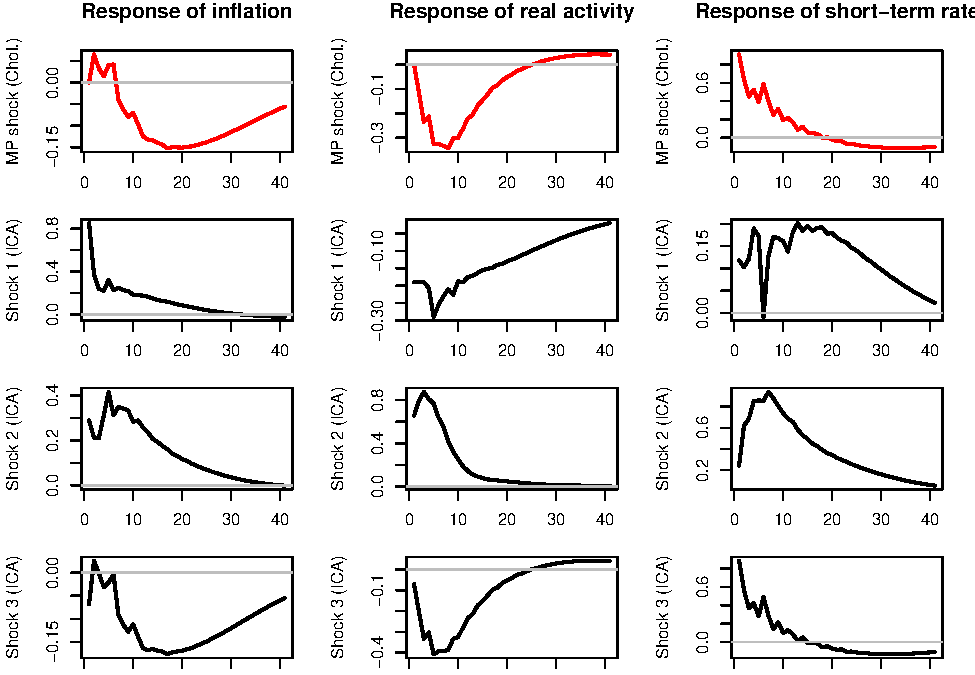
\includegraphics[width=0.95\linewidth]{IdentifStructShocks_files/figure-latex/ICAFigIRF-1} \caption{The first row of plots shows the responses of the three endogenous variables to the monetary policy shock in the context of a Cholesky-idendtified SVAR (ordering: inflation, output gap, interest rate). The next three rows of plots show the repsonses of the endogenous variables to the three structural shocks identified by ICA. The last one (Shock 3) is close to the Cholesky-identified monetary policy shock.}\label{fig:ICAFigIRF}
\end{figure}

According to Figure \ref{fig:ICAFigIRF}, Shock 1 is a supply shock, Shock 2 is a demand shock, and Shock 3 is a monetary-policy shock. Note that Shock 3 is close to the one resulting from the Cholesky approach.
\end{example}

\section{Relation with the Heteroskedasticity Identification}\label{relation-with-the-heteroskedasticity-identification}

In some cases, where the \(\varepsilon_t\)'s are heteroskedastic, the \(B\) matrix can be identified (\citet{Rigobon_2003}, \citet{LANNE2010121}).

Consider the case where we still have \(\varepsilon_t = B \eta_t\) but where \(\eta_t\)'s variance conditionally depends on a regime \(s_t \in \{1,\dots,M\}\). That is:
\[
\mathbb{V}ar(\eta_{k,t}|s_t) = \lambda_{s_t,k} \quad \mbox{for } k \in \{1,\dots,n\}
\]

Denoting by \(\Lambda_i\) the diagonal matrix whose diagonal entries are the \(\lambda_{i,k}\)'s, it comes that:
\[
\mathbb{V}ar(\eta_{t}|s_t) = \Lambda_{s_t},\quad \mbox{and}\quad \mathbb{V}ar(\varepsilon_{t}|s_t) = B\Lambda_{s_t}B'.
\]

Without loss of generality, it can be assumed that \(\Lambda_1=Id\).

In this context, \(B\) is identified, apart from sign reversal of its columns if for all \(k \ne j \in \{1,\dots,n\}\), there is a regime \(i\) s.t. \(\lambda_{i,k} \ne \lambda_{i,j}\). (Prop.1 in \citet{LANNE2010121}).

Bivariate regime case (\(M=2\)): \(B\) identified if the \(\lambda_{2,k}\)'s are all different. That is, identification is ensured if ``there is sufficient heterogeneity in the volatility changes'' (\citet{LUTKEPOHL20172}).

If the regimes \(s_t\) are exogenous and serially independent, then this situation is consistent with the ``non-Gaussian'' situation described above.

\chapter{Local projection methods}\label{Projections}

\section{Overview of the approach}\label{overview-of-the-approach}

Consider the infinite MA representation of \(y_t\) (Eq. \eqref{eq:InfMA}):
\[
y_t = \mu + \sum_{h=0}^\infty \Psi_{h} \eta_{t-h}.
\]
As seen in Section \ref{IRFSVARMA}, the entries \((i,j)\) of the sequence of the \(\Psi_h\) matrices define the IRF of \(\eta_{j,t}\) on \(y_{i,t}\).

Assume that you observe \(\eta_{j,t}\), then a consistent estimate of \(\Psi_{i,j,h}\) is simply obtained by the OLS regression of \(y_{i,t+h}\) on \(\eta_{j,t}\):\footnote{Because the residuals \(u_{i,j,t+h}\) are autocorrelated (for \(h>0\)), estimates of the covariance of the OLS estimators of the \(\Psi_{i,j,h}\) would then have to be based on robust estimators (e.g. \citet{Newey_West_1987}).}
\begin{equation}
y_{i,t+h} = \mu_i + \Psi_{i,j,h}\eta_{j,t} + u_{i,j,t+h}.\label{eq:OLS1}
\end{equation}
Running that kind of regression (using instruments for \(\eta_{j,t}\)) is the core idea of the \textbf{local projection (LP) approach} proposed by \citet{Jorda_2005}.

Now, how to proceed in the (usual) case where \(\eta_{j,t}\) is not observed? We consider two situations. While the second requires some instruments, the first approach does not. This first approach (Section \ref{LPIVww}) is the original \citet{Jorda_2005}'s approach.

\section{Situation A: Without IV}\label{LPIVww}

Assume that the structural shock of interest (\(\eta_{1,t}\), say) can be consistently obtained as the residual of a regression of a variable \(x_t\) on a set of control variables \(w_t\) independent from \(\eta_{1,t}\):
\begin{equation}
\eta_{1,t} = x_t - \mathbb{E}(x_t|w_t),\label{eq:xetaw}
\end{equation}
where \(\mathbb{E}(x_t|w_t)\) is affine in \(w_t\) and where \(w_t\) is an affine transformation of \(\eta_{2:n,t}\) and of past shocks \(\eta_{t-1},\eta_{t-2},\dots\).

Eq. \eqref{eq:xetaw} implies that, conditional on \(w_t\), the additional knowledge of \(x_t\) is useful only when it comes to forecast something that depends on \(\eta_{1,t}\). Hence, given that \(u_{i,1,t+h}\) (see Eq. \eqref{eq:OLS1}) is independent from \(\eta_{1,t}\) (it depends on \(\eta_{t+h},\dots,\eta_{t+1},\color{blue}{\eta_{2:n,t}},\eta_{t-1},\eta_{t-2},\dots\)), it comes that
\begin{equation}
\mathbb{E}(u_{i,1,t+h}|x_t,w_t)= \mathbb{E}(u_{i,1,t+h}|w_t).\label{eq:uuuIV}
\end{equation}
This is the \emph{conditional mean independence} case.

Using \eqref{eq:xetaw}, one can rewrite Eq. \eqref{eq:OLS1} as follows:
\begin{eqnarray*}
y_{i,t+h} &=& \mu_i + \Psi_{i,1,h}\eta_{1,t} + u_{i,1,t+h}\\
&=&  \mu_i + \Psi_{i,1,h}x_t  \color{blue}{-\Psi_{i,1,h}\mathbb{E}(x_t|w_t) + u_{i,1,t+h}},
\end{eqnarray*}

Given Eq. \eqref{eq:uuuIV}, it comes that, conditional on \(x_t\) and \(w_t\), the expectation of the blue term is a function of \(w_t\). Assuming this expectation is linear, standard results in the conditional mean independence case imply that the OLS estimator in the regression of \(y_{i,t+h}\) on \(x_t\), controlling for \(w_t\), provides a consistent estimate of \(\Psi_{i,1,h}\):
\begin{equation}
y_{i,t+h} = \alpha_i + \Psi_{i,1,h}x_t + \beta'w_t + v_{i,t+h}.
\end{equation}

This is for instance consistent with the case where \([\Delta GDP_t, \pi_t,i_t]'\) follows a VAR(1) and the monetary-policy shock does not contemporaneously affect \(\Delta GDP_t\) and \(\pi_t\). The IRFs can then be estimated by LP, taking \(x_t = i_t\) and \(w_t = [\Delta GDP_t,\pi_t,\Delta GDP_{t-1}, \pi_{t-1},i_{t-1}]'\).

This approach closely relates to the SVAR Cholesky-based identification approach. Specifically, if \(w_t = [\color{blue}{y_{1,t},\dots,y_{k-1,t}}, y_{t-1}',\dots,y_{t-p}']'\), with \(k\le n\), and \(x_t = y_{k,t}\), then this approach corresponds, for \(h=0\), to the SVAR(\(p\)) Cholesky-based IRF (focusing on the responses to the \(k^{th}\) structural shock). However, the two approaches differ for \(h>0\), because the LP methodology does not assumes a VAR dynamics for \(y_t\).\footnote{This is reminiscent of the distinction betweem direct forecasting---based on regressions of \(y_{t+h}\) on \(\{y_t,y_{t-1},\dots\}\)---and iterated forecasting---based on a recursive model where \(y_{t+1} = g(y_t,y_{t-1},\dots)+\varepsilon_{t+1}\), see \citet{Marcellino_et_al_2006}.}

In the following lines of code, we employ the \citet{Jorda_2005}'s approach on the same dataset as the one used in Section \ref{Cholesky}. (We were then illustrating \citet{Christiano_Eichenbaum_Evans_1996}'s methodology.)

\begin{Shaded}
\begin{Highlighting}[]
\FunctionTok{library}\NormalTok{(IdSS);}\FunctionTok{library}\NormalTok{(vars)}
\FunctionTok{data}\NormalTok{(}\StringTok{"USmonthly"}\NormalTok{)}
\CommentTok{\# Select sample period:}
\NormalTok{First.date }\OtherTok{\textless{}{-}} \StringTok{"1965{-}01{-}01"}\NormalTok{;Last.date }\OtherTok{\textless{}{-}} \StringTok{"1995{-}06{-}01"}
\NormalTok{indic.first }\OtherTok{\textless{}{-}} \FunctionTok{which}\NormalTok{(USmonthly}\SpecialCharTok{$}\NormalTok{DATES}\SpecialCharTok{==}\NormalTok{First.date)}
\NormalTok{indic.last  }\OtherTok{\textless{}{-}} \FunctionTok{which}\NormalTok{(USmonthly}\SpecialCharTok{$}\NormalTok{DATES}\SpecialCharTok{==}\NormalTok{Last.date)}
\NormalTok{USmonthly   }\OtherTok{\textless{}{-}}\NormalTok{ USmonthly[indic.first}\SpecialCharTok{:}\NormalTok{indic.last,]}
\NormalTok{considered.variables }\OtherTok{\textless{}{-}} \FunctionTok{c}\NormalTok{(}\StringTok{"LIP"}\NormalTok{,}\StringTok{"UNEMP"}\NormalTok{,}\StringTok{"LCPI"}\NormalTok{,}\StringTok{"LPCOM"}\NormalTok{,}\StringTok{"FFR"}\NormalTok{,}\StringTok{"NBR"}\NormalTok{,}\StringTok{"TTR"}\NormalTok{,}\StringTok{"M1"}\NormalTok{)}
\NormalTok{y }\OtherTok{\textless{}{-}} \FunctionTok{as.matrix}\NormalTok{(USmonthly[considered.variables])}
\NormalTok{res.jorda }\OtherTok{\textless{}{-}} \FunctionTok{make.jorda.irf}\NormalTok{(y,}\AttributeTok{posit.of.shock =} \DecValTok{5}\NormalTok{,}
                            \AttributeTok{nb.periods.IRF =} \DecValTok{12}\NormalTok{,}
                            \AttributeTok{nb.lags.endog.var.4.control=}\DecValTok{3}\NormalTok{,}
                            \AttributeTok{indic.plot =} \DecValTok{1}\NormalTok{, }\CommentTok{\# Plots are displayed if = 1.}
                            \AttributeTok{confidence.interval =} \FloatTok{0.90}\NormalTok{)}
\end{Highlighting}
\end{Shaded}

\begin{figure}
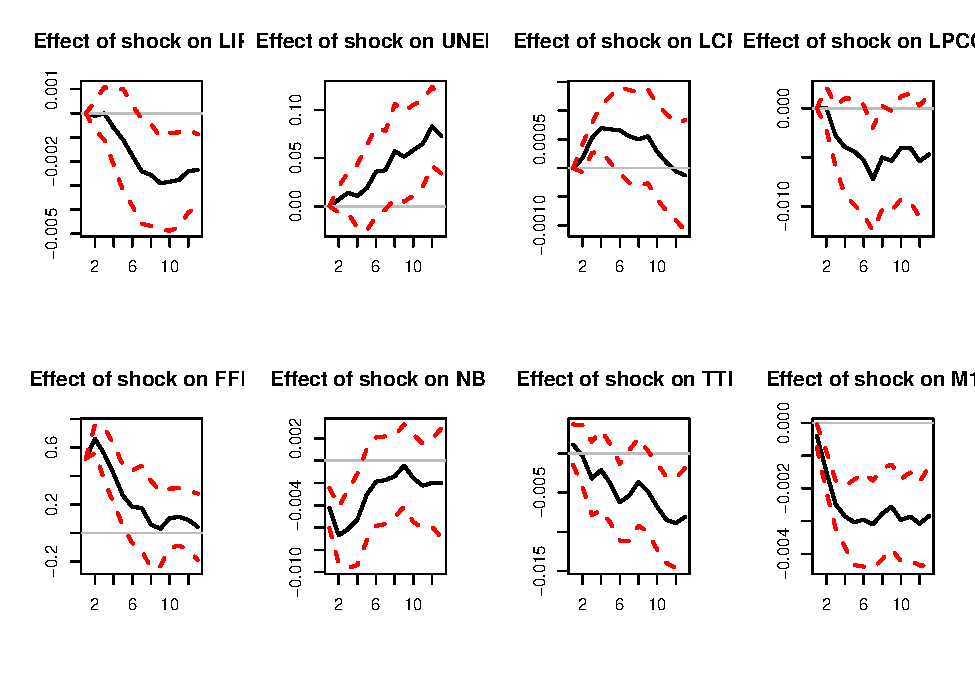
\includegraphics[width=0.95\linewidth]{IdentifStructShocks_files/figure-latex/CEEJorda-1} \caption{Response to a monetary-policy shock. Identification approach of Jorda (2005).}\label{fig:CEEJorda}
\end{figure}

\section{Situation B: IV approach}\label{situation-b-iv-approach}

\subsection{Instruments (proxies for structural shocks)}\label{instruments-proxies-for-structural-shocks}

Consider now that we have a valid instrument \(z_t\) for \(\eta_{1,t}\) (with \(\mathbb{E}(z_t)=0\)). That is:
\begin{equation}
\left\{
\begin{array}{llll}
(IV.i) & \mathbb{E}(z_t \eta_{1,t}) &\ne 0 & \mbox{(relevance condition)} \\
(IV.ii) & \mathbb{E}(z_t \eta_{j,t}) &= 0 \quad \mbox{for } j>1 & \mbox{(exogeneity condition).}
\end{array}\right.\label{eq:IV1}
\end{equation}
The instrument \(z_t\) can be used to identify the structural shock. Eq. \eqref{eq:IV1} implies that there exist \(\rho \ne 0\) and a mean-zero variable \(\xi_t\) such that:
\[
\eta_{1,t} = \rho z_t + \xi_t,
\]
where \(\xi_t\) is correlated neither to \(z_t\), nor to \(\eta_{j,t}\), \(j\ge2\).

\begin{proof}
Define \(\rho = \frac{\mathbb{E}(\eta_{1,t}z_t)}{\mathbb{V}ar(z_t)}\) and \(\xi_t = \eta_{1,t} - \rho z_t\). It is easily seen that \(\xi_t\) satisfies the moment restrictions given above.
\end{proof}

\citet{Ramey_2016_NBER} reviews the different approaches employed to construct monetary policy-shocks (the two main approaches are presented in \ref{exm:HighFreq} and \ref{exm:RomerRomer} below). She has also collected time series of such shocks, see \href{https://econweb.ucsd.edu/~vramey/research.html\#mon}{her website}. Several of these shocks are included in the \texttt{Ramey} dataset of package \texttt{IdSS}.

\begin{example}[Identification of Monetary-Policy Shocks Based on High-Frequency Data]
\protect\hypertarget{exm:HighFreq}{}\label{exm:HighFreq}

Instruments for monetary-policy shocks can be extracted from high-frequency market data associated with interest-rate products.

The quotes of all interest-rate-related financial products are sensitive to monetary-policy announcements. That is because these quotes mainly depends on investors' expectations regarding future short-term rates: \(\mathbb{E}_t(i_{t+s})\). Typically, if agents were risk-neutral, the maturity-\(h\) interest rate would approximatively be given by:
\[
i_{t,h} \approx \mathbb{E}_t\left(\frac{1}{h}\int_{0}^{h} i_{t+s} ds\right) = \frac{1}{h}\int_{0}^{h} \mathbb{E}_t\left(i_{t+s}\right) ds.
\]
In general, changes in \(\mathbb{E}_t(i_{t+s})\), for \(s>0\), can be affected by all types of shocks that may trigger a reaction by the central bank.

However, if a MP announcement takes place between \(t\) and \(t+\epsilon\), then most of \(\mathbb{E}_{t+\epsilon}(i_{t+s})-\mathbb{E}_t(i_{t+s})\) is to be attributed to the MP shock (see Figure \ref{fig:HighFreq}, from \citet{Gurkaynak_et_al_2005}). Hence, a monthly time series of MP shocks can be obtained by summing, over each month, the changes \(i_{t+ \epsilon,h} - i_{t,h}\) associated with a given interest rate (T-bills, futures, swaps) and a given maturity \(h\).

See among others: \citet{KUTTNER2001523}, \citet{Cochrane_Piazzesi_2002}, \citet{Gurkaynak_et_al_2005}, \citet{Piazzesi_Swanson_2008}, \citet{Gertler_Karadi_2015}. The time series named
\texttt{FF4\_TC}, \texttt{ED2\_TC}, \texttt{ED3\_TC}, \texttt{ED4\_TC}, \texttt{GS1}, \texttt{ff1\_vr}, \texttt{ff4\_vr}, \texttt{ed2\_vr}, \texttt{ff1\_gkgreen}, \texttt{ff4\_gkgreen}, \texttt{ed2\_gkgreen} in the data frame \texttt{Ramey} of package \texttt{IdSS} are time series of shocks based on this approach (see \href{https://econweb.ucsd.edu/~vramey/research/Ramey_HOM_monetary.zip}{Ramey's website} for details).

\begin{figure}
\includegraphics[width=0.95\linewidth]{images/GSS2005_HFI} \caption{Source: Gurkaynak, Sack and Swanson (2005). Transaction rates of Federal funds futures on June 25, 2003, day on which a regularly scheduled FOMC meeting was scheduled. At 2:15 p.m., the FOMC announced that it was lowering its target for the federal funds rate from 1.25\% to 1\%, while many market participants were expecting a 50 bp cut. This shows that (i) financial markets seem to fully adjust to the policy action within just a few minutes and (ii) the federal funds rate surprise is not necessarily in the same direction as the federal funds rate action itself.}\label{fig:HighFreq}
\end{figure}

\end{example}

\begin{example}[Identification of Monetary-Policy Shocks Based on the Narrative Approach]
\protect\hypertarget{exm:RomerRomer}{}\label{exm:RomerRomer}\citet{Romer_Romer_2004} propose a two-step approach:

\begin{enumerate}
\def\labelenumi{\alph{enumi}.}
\tightlist
\item
  derive a series for Federal Reserve intentions for the federal funds rate (the explicit target of the Fed) around FOMC meetings,
\item
  control for Federal Reserve forecasts.
\end{enumerate}

This gives a measure of intended monetary policy actions not driven by information about future economic developments.

\begin{enumerate}
\def\labelenumi{\alph{enumi}.}
\tightlist
\item
  ``intentions'' are measured as a combination of narrative and quantitative evidence. Sources: (among others) Minutes of FOMC and ``Blue Books''.
\item
  Controls = variables spanning the information the Federal Reserve has about future developments. Data: Federal Reserve's internal forecasts (inflation, real output and unemployment), ``Greenbook's forecasts'' -- usually issued 6 days before the FOMC meeting.
\end{enumerate}

The shock measure is the residual series in the linear regression of (a) on (b). The time series \texttt{Ramey\$rrshock83} and \texttt{Ramey\$rrshock83b} (where \texttt{Ramey} is a data frame included in package \texttt{IdSS}) contain such shocks for the period 1983-2007. (\texttt{Ramey\$rrshock83b} uses long-horizon Greenbook forecasts.)
\end{example}

To create a measure of \emph{news} about future government spending, \citet{Ramey_2011} uses newspaper articles to construct a time series of (unexpected) fiscal shocks:\footnote{Data and replication codes can be found on \href{https://econweb.ucsd.edu/~vramey/research.html\#govt}{her website}.}

\begin{example}[Identification of news about future government spending]
\protect\hypertarget{exm:RameyQJE2011}{}\label{exm:RameyQJE2011}

\citet{Ramey_2011}'s measure aims to measure the expected discounted value of government spending changes due to foreign political events. She argues this variable should matter for the wealth effect in a neoclassical framework. The series is constructed by reading periodicals in order to gauge the public's expectations (\emph{Business Week} before 2001, other newspapers afterwards).

According to \citet{Ramey_2011}, government sources could not be used because (a) they were either not released in a timely manner or (b) were known to underestimate the costs of certain actions.

Figure \ref{fig:RameyFiscalShocks} shows the resulting time series of shocks. Figure \ref{fig:IRFfiscalRamey} shows the IRF of macro variables to the shock on expected government spending.

\begin{figure}
\includegraphics[width=0.95\linewidth]{images/RameyFiscalShocks} \caption{Source: Ramey (2011). Defense News: PDV of Change in Spending as a Percent of GDP.}\label{fig:RameyFiscalShocks}
\end{figure}

\begin{figure}
\includegraphics[width=0.95\linewidth]{images/RameyFiscalShocksIRF} \caption{Source: Ramey (2011) [Figure X of the paper]. Responses of macro variables to a shock on expected government spending.}\label{fig:IRFfiscalRamey}
\end{figure}

\end{example}

There are two main IV approaches to estimate IRFs see \citet{Stock_Watson_2018}:

\begin{enumerate}
\def\labelenumi{\alph{enumi}.}
\tightlist
\item
  The SVAR-IV approach (Subsection \ref{SVARIVa}),
\item
  The LP-IV approach, where \(y_t\)'s DGP is left unspecified (Subsection \ref{LPIVa}).
\end{enumerate}

The LP-IV approach is based on a set of IV regressions (for each variable of interest, one for each forecast horizon). The SVAR-IV approach is based on IV regressions of VAR innovations only (one for each series of VAR innovations).

If the VAR adequately captures the DGP, then the IV-SVAR is optimal for all horizons. However, if the VAR is misspecified, then specification errors are compounded at each horizon and a local projection method would lead to better results.

\subsection{Situation B.1: SVAR-IV approach}\label{SVARIVa}

Assume you have consistent estimates of \(\varepsilon_t = B\eta_t\), these estimates (\(\hat\varepsilon_{t}\)) coming from the estimation of a VAR model. We have, for \(i \in \{1,\dots,n\}\):
\begin{eqnarray}
\varepsilon_{i,t} &=& b_{i,1} \eta_{1,t} + u_{i,t} \label{eq:epsrho}\\
&=& b_{i,1} \rho z_t + \underbrace{b_{i,1}\xi_t + u_{i,t}}_{\perp z_t}. \nonumber
\end{eqnarray}
(\(u_{i,t}\) is a linear combination of the \(\eta_{j,t}\)'s, \(j\ge2\)).

Hence, up to a multiplicative factor (\(\rho\)), the (OLS) regressions of the \(\hat\varepsilon_{i,t}\)'s on \(z_t\) (that are consistent of the true \(\varepsilon_{i,t}\)'s) provide consistent estimates of the \(b_{i,1}\)'s.

Combined with the estimated VAR (the \(\Phi_k\) matrices), this provides consistent estimates of the IRFs of \(\eta_{1,t}\) on \(y_t\), though up to a multiplicative factor. This scale ambiguity can be solved by rescaling the structural shock (``unit-effect normalisation'', see \citet{Stock_Watson_2018}). Let us consider \(\tilde\eta_{1,t}=b_{1,1}\eta_{1,t}\); by construction, \(\tilde\eta_{1,t}\) has a unit contemporaneous effect on \(y_{1,t}\). Denoting by \(\tilde{B}_{i,1}\) the contemporaneous impact of \(\tilde\eta_{1,t}\) on the \(i^{th}\) endogenous variable, we get:
\[
\tilde{B}_{1} = \frac{1}{b_{1,1}} {B}_{1},
\]
where \(B_{1}\) denotes the \(1^{st}\) column of \(B\) and \(\tilde{B}_{1}=[1,\tilde{B}_{2,1},\dots,\tilde{B}_{n,1}]'\).

Eq. \eqref{eq:epsrho} gives:
\begin{eqnarray*}
\varepsilon_{1,t} &=& \tilde\eta_{1,t} + u_{1,t}\\
\varepsilon_{i,t} &=& \tilde{B}_{i,1} \tilde\eta_{1,t} + u_{i,t}.
\end{eqnarray*}
This suggests that \(\tilde{B}_{i,1}\) can be estimated by regressing \(\varepsilon_{i,t}\) on \(\varepsilon_{1,t}\) (or \(\hat\varepsilon_{i,t}\) on \(\hat\varepsilon_{1,t}\) in practice), using \(z_t\) as an instrument.

What about inference? Once cannot use the usual TSLS standard deviations because the \(\varepsilon_{i,t}\)'s are not directly observed. Bootstrap procedures can be resorted to. \citet{Stock_Watson_2018} propose, in particular, a Gaussian parametric bootstrap:

Assume you have estimated \(\{\widehat{\Phi}_1,\dots,\widehat{\Phi}_p,\widehat{B}_1\}\) using the SVAR-IV approach based on a size-\(T\) sample. Generate \(N\) (where \(N\) is large) size-\(T\) samples from the following VAR:
\[
\left[
\begin{array}{cc}
\widehat{\Phi}(L) & 0 \\
0 & \widehat{\rho}(L)
\end{array}
\right]
\left[
\begin{array}{c}
y_t \\
z_t
\end{array}
\right] =
\left[
\begin{array}{c}
\varepsilon_t \\
e_t
\end{array}
\right],
\]
\[
\mbox{where} \quad \left[
\begin{array}{c}
\varepsilon_t \\
e_t
\end{array}
\right]\sim \, i.i.d.\,\mathcal{N}\left(\left[\begin{array}{c}0\\0\end{array}\right],
\left[\begin{array}{cc}
\Omega & S'_{\varepsilon,e}\\
S_{\varepsilon,e}& \sigma^2_{e}
\end{array}\right]
\right),
\]
where \(\widehat{\rho}(L)\) and \(\sigma^2_{e}\) result from the estimation of an AR process for \(z_t\), and where \(\Omega\) and \(S_{\varepsilon,e}\) are sample covariances for the VAR/AR residuals.

For each simulated sample (of \(\tilde{y}_t\) and \(\tilde{z}_t\), say), estimate \(\{\widetilde{\widehat{\Phi}}_1,\dots,\widetilde{\widehat{\Phi}}_p,\widetilde{\widehat{B}}_1\}\) and associated \(\widetilde{\Psi}_{i,1,h}\). This provides e.g.~a sequence of \(N\) estimates of \(\Psi_{i,1,h}\), from which quantiles and conf. intervals can be deduced.

In the following lines of code, we use this approach to estimate the response of macroeconomic variables to a monetary policy shock. The instrument is \texttt{FF4\_TC} from the Ramsey's database; they are base on the \citet{Gertler_Karadi_2015} approach, that use 3-month fed funds futures.

\begin{Shaded}
\begin{Highlighting}[]
\FunctionTok{library}\NormalTok{(vars);}\FunctionTok{library}\NormalTok{(IdSS)}
\FunctionTok{data}\NormalTok{(}\StringTok{"USmonthly"}\NormalTok{)}
\NormalTok{First.date }\OtherTok{\textless{}{-}} \StringTok{"1990{-}05{-}01"}\NormalTok{;Last.date }\OtherTok{\textless{}{-}} \StringTok{"2012{-}6{-}01"}
\NormalTok{indic.first }\OtherTok{\textless{}{-}} \FunctionTok{which}\NormalTok{(USmonthly}\SpecialCharTok{$}\NormalTok{DATES}\SpecialCharTok{==}\NormalTok{First.date)}
\NormalTok{indic.last  }\OtherTok{\textless{}{-}} \FunctionTok{which}\NormalTok{(USmonthly}\SpecialCharTok{$}\NormalTok{DATES}\SpecialCharTok{==}\NormalTok{Last.date)}
\NormalTok{USmonthly   }\OtherTok{\textless{}{-}}\NormalTok{ USmonthly[indic.first}\SpecialCharTok{:}\NormalTok{indic.last,]}
\NormalTok{shock.name }\OtherTok{\textless{}{-}} \FunctionTok{c}\NormalTok{(}\StringTok{"FF4\_TC"}\NormalTok{,}\StringTok{"ED2\_TC"}\NormalTok{) }\CommentTok{\# "ff1\_vr", "rrshock83b"}
\NormalTok{indic.shock.name }\OtherTok{\textless{}{-}} \FunctionTok{which}\NormalTok{(}\FunctionTok{names}\NormalTok{(USmonthly)}\SpecialCharTok{\%in\%}\NormalTok{shock.name)}
\NormalTok{Z }\OtherTok{\textless{}{-}} \FunctionTok{as.matrix}\NormalTok{(USmonthly[,indic.shock.name])}
\FunctionTok{par}\NormalTok{(}\AttributeTok{plt=}\FunctionTok{c}\NormalTok{(.}\DecValTok{1}\NormalTok{,.}\DecValTok{95}\NormalTok{,.}\DecValTok{1}\NormalTok{,.}\DecValTok{95}\NormalTok{))}
\FunctionTok{plot}\NormalTok{(USmonthly}\SpecialCharTok{$}\NormalTok{DATES,Z[,}\DecValTok{1}\NormalTok{],}\AttributeTok{type=}\StringTok{"l"}\NormalTok{,}\AttributeTok{xlab=}\StringTok{""}\NormalTok{,}\AttributeTok{ylab=}\StringTok{""}\NormalTok{,}\AttributeTok{lwd=}\DecValTok{2}\NormalTok{)}
\FunctionTok{lines}\NormalTok{(USmonthly}\SpecialCharTok{$}\NormalTok{DATES,Z[,}\DecValTok{2}\NormalTok{],}\AttributeTok{col=}\StringTok{"red"}\NormalTok{,}\AttributeTok{lwd=}\DecValTok{2}\NormalTok{,}\AttributeTok{pch=}\DecValTok{3}\NormalTok{,}\AttributeTok{lty=}\DecValTok{2}\NormalTok{)}
\end{Highlighting}
\end{Shaded}

\begin{figure}
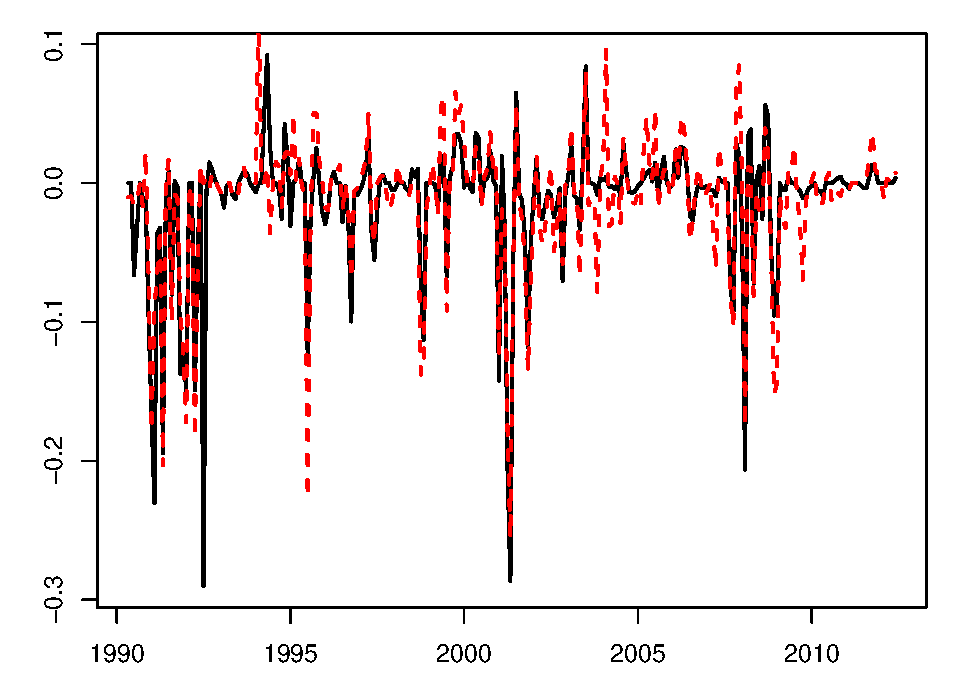
\includegraphics[width=0.95\linewidth]{IdentifStructShocks_files/figure-latex/essaiIV0-1} \caption{Gertler-Karadi monthly shocks, fed funds futures 3 months (resp. 6 months) in black (resp. in red).}\label{fig:essaiIV0}
\end{figure}

\begin{Shaded}
\begin{Highlighting}[]
\NormalTok{considered.variables }\OtherTok{\textless{}{-}} \FunctionTok{c}\NormalTok{(}\StringTok{"GS1"}\NormalTok{,}\StringTok{"LIP"}\NormalTok{,}\StringTok{"LCPI"}\NormalTok{,}\StringTok{"EBP"}\NormalTok{)}
\NormalTok{Y }\OtherTok{\textless{}{-}} \FunctionTok{as.matrix}\NormalTok{(USmonthly[,considered.variables])}
\NormalTok{n }\OtherTok{\textless{}{-}} \FunctionTok{length}\NormalTok{(considered.variables)}
\FunctionTok{colnames}\NormalTok{(Y) }\OtherTok{\textless{}{-}}\NormalTok{ considered.variables}
\FunctionTok{par}\NormalTok{(}\AttributeTok{plt=}\FunctionTok{c}\NormalTok{(.}\DecValTok{15}\NormalTok{,.}\DecValTok{95}\NormalTok{,.}\DecValTok{15}\NormalTok{,.}\DecValTok{8}\NormalTok{))}
\NormalTok{res.svar.iv }\OtherTok{\textless{}{-}} 
  \FunctionTok{svar.iv}\NormalTok{(Y,Z,}\AttributeTok{p =} \DecValTok{4}\NormalTok{,}\AttributeTok{names.of.variables=}\NormalTok{considered.variables,}
          \AttributeTok{nb.periods.IRF =} \DecValTok{20}\NormalTok{,}
          \AttributeTok{z.AR.order=}\DecValTok{1}\NormalTok{, }
          \AttributeTok{nb.bootstrap.replications =} \DecValTok{100}\NormalTok{, }
          \AttributeTok{confidence.interval =} \FloatTok{0.90}\NormalTok{,}
          \AttributeTok{indic.plot=}\DecValTok{1}\NormalTok{)}
\end{Highlighting}
\end{Shaded}

\begin{figure}
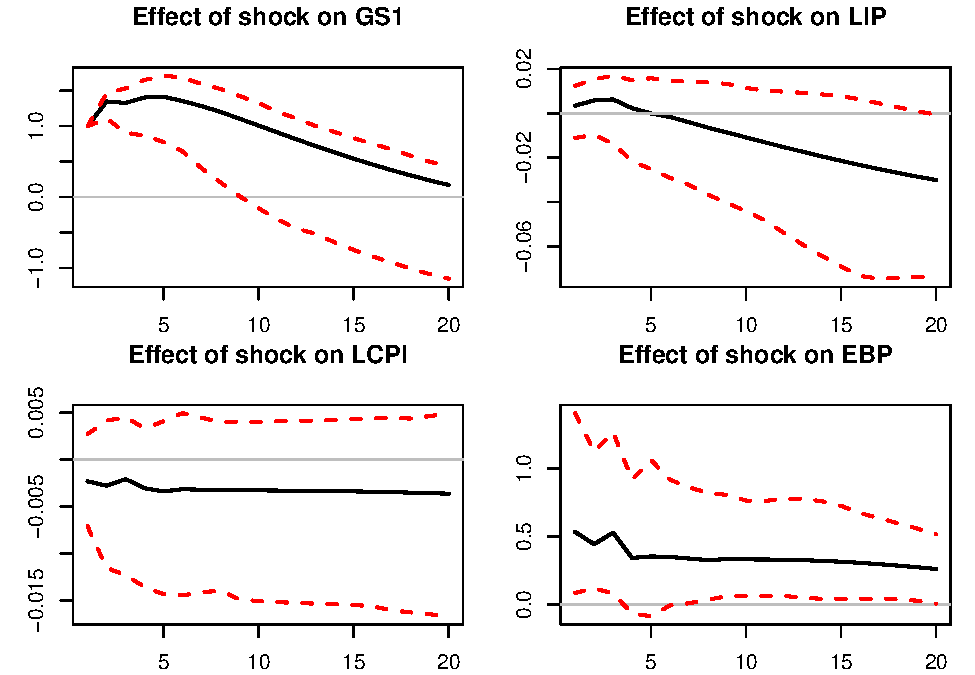
\includegraphics[width=0.95\linewidth]{IdentifStructShocks_files/figure-latex/essaiIV1-1} \caption{Reponses to a monetary-policy shock, SVAR-IV approach.}\label{fig:essaiIV1}
\end{figure}

\subsection{Situation B.2: LP-IV}\label{LPIVa}

If you do not want to posit a VAR-type dynamics for \(y_t\) --e.g., because you suspect that the true generating model may be a non-invertible VARMA model-- you can directly proceed by IV-projection methods to obtain the \(\tilde\Psi_{i,1,h}\equiv \Psi_{i,1,h}/b_{1,1}\) (that are the IRFs of \(\tilde\eta_{1,t}\) on \(y_{i,t}\)).

However, Assumptions (IV.i) and (IV.ii) (Eq. \eqref{eq:IV1}) have to be complemented with (IV.iii):
\begin{equation*}
\begin{array}{llll}
(IV.iii) & \mathbb{E}(z_t \eta_{j,t+h}) &= 0 \, \mbox{ for } h \ne 0 & \mbox{(lead-lag exogeneity)}
\end{array}
\end{equation*}

When (IV.i), (IV.ii) and (IV.iii) are satisfied, \(\tilde\Psi_{i,1,h}\) can be estimated by regressing \(y_{i,t+h}\) on \(y_{1,t}\), using \(z_t\) as an instrument, i.e.~by considering the TSLS estimation of:
\begin{equation}
y_{i,t+h} = \alpha_i + \tilde\Psi_{i,1,h}y_{1,t} + \nu_{i,t+h},\label{eq:regIV1}
\end{equation}
where \(\nu_{i,t+h}\) is correlated to \(y_{1,t}\), but not to \(z_t\).

We have indeed:
\begin{eqnarray*}
y_{1,t} &=& \alpha_1 + \tilde\eta_{1,t} + v_{1,t}\\
y_{i,t+h} &=& \alpha_i + \tilde\Psi_{i,1,h}\tilde\eta_{1,t} + v_{i,t+h},
\end{eqnarray*}
where the \(v_{i,t+h}\)'s are uncorrelated to \(z_t\) under (IV.i), (IV.ii) and (IV.iii).

Note again that, for \(h>0\), the \(v_{i,t+h}\) (and \(\nu_{i,t+h}\)) are auto-correlated. Newey-West corrections therefore have to be used to compute std errors of the \(\tilde\Psi_{i,1,h}\)'s estimates.

Consider the linear regression:
\[
\mathbf{Y} = \mathbf{X}\boldsymbol\beta + \boldsymbol\varepsilon,
\]
where \(\mathbb{E}(\boldsymbol\varepsilon)=0\), but where the explicative variables \(\mathbf{X}\) can be correlated to the residuals \(\boldsymbol\varepsilon\). Moreover, the \(\boldsymbol\varepsilon\)'s may feature heteroskedasticity and be auto-correlated. We denote by \(\mathbf{Z}\) the matrix of instruments, with \(\mathbb{E}(\mathbf{X}'\mathbf{Z}) \ne 0\) but \(\mathbb{E}(\boldsymbol\varepsilon'\mathbf{Z}) = 0\).

The IV estimator of \(\boldsymbol\beta\) is obtained by regressing \(\hat{\mathbf{Y}}\) on \(\hat{\mathbf{X}}\), where \(\hat{\mathbf{Y}}\) and \(\hat{\mathbf{X}}\) are the respective residuals of the regressions of \(\mathbf{Y}\) and \(\mathbf{X}\) on \(\mathbf{Z}\).
\begin{eqnarray*}
\mathbf{b}_{iv} &=& [\mathbf{X}'\mathbf{Z}(\mathbf{Z}'\mathbf{Z})^{-1}\mathbf{Z}'\mathbf{X}]^{-1}\mathbf{X}'\mathbf{Z}(\mathbf{Z}'\mathbf{Z})^{-1}\mathbf{Z}'\mathbf{Y}\\
\mathbf{b}_{iv} &=& \boldsymbol\beta + \frac{1}{\sqrt{T}}\underbrace{T[\mathbf{X}'\mathbf{Z}(\mathbf{Z}'\mathbf{Z})^{-1}\mathbf{Z}'\mathbf{X}]^{-1}\mathbf{X}'\mathbf{Z}(\mathbf{Z}'\mathbf{Z})^{-1}}_{=Q(\mathbf{X},\mathbf{Z}) \overset{p}{\rightarrow} \mathbf{Q}_{xz}}\underbrace{\sqrt{T}\left(\frac{1}{T}\mathbf{Z}'\boldsymbol\varepsilon\right)}_{\overset{d}{\rightarrow} \mathcal{N}(0,S)},
\end{eqnarray*}
where \(\mathbf{S}\) is the long-run variance of \(\mathbf{z}_t\varepsilon_t\).\footnote{That is the sum of the covariance matrices of \(\mathbf{z}_t\varepsilon_t\), for orders from \(-\infty\) to \(+\infty\).} The asymptotic covariance matrix of \(\sqrt{T}\mathbf{b}_{iv}\) is \(\mathbf{Q}_{xz} \mathbf{S} \mathbf{Q}_{xz}'\). Therefore, the covariance matrix of \(\mathbf{b}_{iv}\) can be approximated by \(\frac{1}{T}Q(\mathbf{X},\mathbf{Z})\hat{\mathbf{S}}Q(\mathbf{X},\mathbf{Z})'\) where \(\hat{\mathbf{S}}\) is the Newey-West estimator of \(\mathbf{S}\).\footnote{That is: \(\hat{\mathbf{S}}=\hat\gamma_0 + 2 \sum_{\nu=1}^{q}\left(1-\frac{\nu}{q+1}\right) \hat\gamma_\nu\), where the \(\hat\gamma_j\)'s are sample auto-covariances of \(\mathbf{z}_t\varepsilon_t\), see \citet{Newey_West_1987}}

Assumption (IV.iii) is usually not restrictive for \(h>0\) (\(z_t\) is usually not affected by future shocks). By contrast, it may be restrictive for \(h<0\). This can be solved by adding controls in Regression \eqref{eq:regIV1}. These controls should span the space of \(\{\eta_{t-1},\eta_{t-2},\dots\}\).

If \(z_t\) is suspected to be correlated to past values of \(\eta_{1,t}\) but not to the \(\eta_{j,t}\)'s, \(j>1\), then one can add lags of \(z_t\) as controls (method e.g.~advocated by Ramey, 2016, p.108, considering the instrument by \citet{Gertler_Karadi_2015}).

In the general case, one can use lags of \(y_t\) as controls. Note that, even if (IV.iii) holds, adding controls may reduce the variance of the regression error.

\begin{Shaded}
\begin{Highlighting}[]
\NormalTok{res.LP.IV }\OtherTok{\textless{}{-}} \FunctionTok{make.LPIV.irf}\NormalTok{(Y,Z,}
                           \AttributeTok{nb.periods.IRF =} \DecValTok{20}\NormalTok{,}
                           \AttributeTok{nb.lags.Y.4.control=}\DecValTok{4}\NormalTok{,}
                           \AttributeTok{nb.lags.Z.4.control=}\DecValTok{4}\NormalTok{,}
                           \AttributeTok{indic.plot =} \DecValTok{1}\NormalTok{, }\CommentTok{\# Plots are displayed if = 1.}
                           \AttributeTok{confidence.interval =} \FloatTok{0.90}\NormalTok{)}
\end{Highlighting}
\end{Shaded}

\chapter{Panel VARs}\label{PanelVARs}

Panel VARs have the same structure as VAR models, in the
sense that all variables are assumed to be endogenous and
interdependent, but a \emph{cross sectional dimension} is
added to the representation. There are \(N\) units indexed by
\(i\in\{1,...,N\}\). The index \(i\) is generic and could indicate
countries, sectors, markets\ldots{} Then a panel VAR is
\[ y_{it}=c_i+\Phi_i(L)
y_{t-1}+\varepsilon_{it}.\] where \(y_t\) is the stacked version of
\(y_{it}\) and \(\varepsilon_t\) is i.i.d., with variance-covariance
matrix \(\Omega\). Vector \(c_i\) and the lag polynomial \(\Phi_i(L)\) may depend on the unit. \citet{Canova_Cicarelli_2013} provide a survey of panel estimation methods.

Contrary to standard VARs, panel VARs may help study
* similarities/differences in the transmission of shocks;
* Spillovers, contagion.

But panel VARs are subject tothe \emph{curse of dimensionality}. Indeed, they can be characterized by
* \emph{Dynamic interdependence}: potentially, the lags of \emph{all}
endogenous variables of \emph{all} units can enter the model for unit \(i\).
* \emph{Static interdependence}: \(\varepsilon_{it}\) are
generally correlated across \(i\).
* \emph{Cross sectional heterogeneity}: the intercept, the slope and the
variance of the shocks may be unit-specific.

\section{Without Dynamic interdependence}\label{without-dynamic-interdependence}

A panel VAR, assuming no dynamic interdependence, is of the form:
\[ y_{it}=c_i+\Phi_i(L)
\color{red}{y_{it-1}}+\varepsilon_{it}.\]

As a comparison, consider \emph{micro panel data}, in the univariate cae (AR(1) case): \[y_{it}=c_i+{\color{red}\phi} y_{it-1}+\varepsilon_{it}.\] In that kind of context, we usually have no cross-sectional heterogeneity as \(\phi_i=\phi\) for all \(i\). Typically, we have a large cross-sectional dimension \(N\), and a small time dimension \(T\). If one uses a \emph{``Fixed-effect'\,' regression}:
\[y_{it}-\frac{1}{T}\sum_{s=1}^Ty_{is}=\phi(y_{it-1}-\frac{1}{T}\sum_{s=1}^Ty_{is})+\varepsilon_{it}-\frac{1}{T}\sum_{s=1}^T\color{red}{\varepsilon_{is}},\]
then one faces the \emph{Nickell bias}: with a lagged dependent variable, the estimator is biased, with a bias of size \(\sim 1/T\). One can then use GMM regressions (\citet{Arellano_Bond_1991}) so as to get unbiased estimates.

\emph{Macro panel data} have a different structure, with typically a moderate cross-sectional dimension \(N\) and a large time dimension \(T\), so that the Nickell bias is negligible (\(\rightarrow 0\) as \(T\rightarrow\infty\)).

\subsection{Mean Group Estimator}\label{mean-group-estimator}

When we etimate
\[ y_{it}=c_i+\Phi_i(L)
y_{it-1}+\varepsilon_{it},\]
we need to take into account the cross-sectional heterogeneity in the coefficients, i.e., different \(\Phi_i\)'s across \(i\)'s.
Pooled estimators (assuming cross-sectional homogeneity, i.e.~identical \(\Phi_i\)'s across \(i\)s) are \emph{not consistent} (biased) if the underlying dynamics are actually heterogeneous. By contrast, the \emph{Mean Group (MG) estimator}, which consists in estimating \(N\) separate regressions
and calculating the coefficient means, is \emph{consistent}.

\subsection{Shock identification}\label{shock-identification}

Shock identification can be performed with standard methods (zeros, signs, FEVM, etc.). We make the assumption that \(\Omega\) is block-diagonal (no interdependence on impact), which is consistent with the assumption of no cross-sectional dependence.

\section{With Dynamic Interdependencies}\label{with-dynamic-interdependencies}

A panel VAR that accommodates dynamic interdependence is of the form:
\[ y_{it}=c_i+\Phi_i(L)
y_{t-1}+\varepsilon_{it}.\]

We face a serious \emph{curse of dimensionality} here: there are \(NGp+1\) coefficients to estimate in
each equation.

A solution is to select some eligible dynamic links (See for instance \citet{DelNegro_Schorfheide_2010}). Another alternative is to use a factor model. This consists in capturing the dynamic interdependencies by a set of unobservable factors (See \citet{Canova_Cicarelli_2004} and \citet{Canova_Cicarelli_2009}). See Section \ref{FAVAR} for more details on FAVAR models.

\chapter{Factor-Augmented VAR}\label{FAVAR}

VAR models are subject to the curse of dimensionality: If \(n\), is large, then the number of parameters (in \(n^2\)) explodes.

In the case where one suspects that the \(y_{i,t}\)'s are mainly driven by a small number of random sources, a factor structure may be imposed, and \textbf{principal component analysis} (PCA, see Appendix \ref{PCAapp}) can be employed to estimate the relevant factors (\citet{Bernanke_Boivin_Eliasz_2005}).

\section{Principal component analysis (PCA)}\label{PCAapp}

\textbf{Principal component analysis (PCA)} is a classical and easy-to-use statistical method to reduce the dimension of large datasets containing variables that are linearly driven by a relatively small number of factors. This approach is widely used in data analysis and image compression.

Suppose that we have \(T\) observations of a \(n\)-dimensional random vector \(x\), denoted by \(x_{1},x_{2},\ldots,x_{T}\). We suppose that each component of \(x\) is of mean zero.

Let denote with \(X\) the matrix given by \(\left[\begin{array}{cccc}
x_{1} & x_{2} & \ldots & x_{T}\end{array}\right]'\). Denote the \(j^{th}\) column of \(X\) by \(X_{j}\).

We want to find the linear combination of the \(x_{i}\)'s (\(x.u\)), with \(\left\Vert u\right\Vert =1\), with ``maximum variance.'' That is, we want to solve:
\begin{equation}
\begin{array}{clll}
\underset{u}{\arg\max} & u'X'Xu. \\
\mbox{s.t. } & \left\Vert u \right\Vert =1
\end{array}\label{eq:PCA11}
\end{equation}

Since \(X'X\) is a positive definite matrix, it admits the following decomposition:
\begin{eqnarray*}
X'X & = & PDP'\\
& = & P\left[\begin{array}{ccc}
\lambda_{1}\\
& \ddots\\
&  & \lambda_{n}
\end{array}\right]P',
\end{eqnarray*}
where \(P\) is an orthogonal matrix whose columns are the eigenvectors of \(X'X\).

We can order the eigenvalues such that \(\lambda_{1}\geq\ldots\geq\lambda_{n}\). (Since \(X'X\) is positive definite, all these eigenvalues are positive.)

Since \(P\) is orthogonal, we have \(u'X'Xu=u'PDP'u=y'Dy\) where \(\left\Vert y\right\Vert =1\). Therefore, we have \(y_{i}^{2}\leq 1\) for any \(i\leq n\).

As a consequence:
\[
y'Dy=\sum_{i=1}^{n}y_{i}^{2}\lambda_{i}\leq\lambda_{1}\sum_{i=1}^{n}y_{i}^{2}=\lambda_{1}.
\]

It is easily seen that the maximum is reached for \(y=\left[1,0,\cdots,0\right]'\). Therefore, the maximum of the optimization program (Eq. \eqref{eq:PCA11}) is obtained for \(u=P\left[1,0,\cdots,0\right]'\). That is, \(u\) is the eigenvector of \(X'X\) that is associated with its larger eigenvalue (first column of \(P\)).

Let us denote with \(F\) the vector that is given by the matrix product \(XP\). The columns of \(F\), denoted by \(F_{j}\), are called \textbf{factors}. We have:
\[
F'F=P'X'XP=D.
\]
Therefore, in particular, the \(F_{j}\)'s are orthogonal.

Since \(X=FP'\), the \(X_{j}\)'s are linear combinations of the factors. Let us then denote with \(\hat{X}_{i,j}\) the part of \(X_{i}\) that is explained by factor \(F_{j}\), we have:
\begin{eqnarray*}
\hat{X}_{i,j} & = & p_{ij}F_{j}\\
X_{i} & = & \sum_{j}\hat{X}_{i,j}=\sum_{j}p_{ij}F_{j}.
\end{eqnarray*}

Consider the share of variance that is explained---through the \(n\) variables (\(X_{1},\ldots,X_{n}\))---by the first factor \(F_{1}\):
\begin{eqnarray*}
\frac{\sum_{i}\hat{X}'_{i,1}\hat{X}_{i,1}}{\sum_{i}X_{i}'X_{i}} & = & \frac{\sum_{i}p_{i1}F'_{1}F_{1}p_{i1}}{tr(X'X)} = \frac{\sum_{i}p_{i1}^{2}\lambda_{1}}{tr(X'X)} = \frac{\lambda_{1}}{\sum_{i}\lambda_{i}}.
\end{eqnarray*}

Intuitively, if the first eigenvalue is large, it means that the first factor captures a large share of the fluctutaions of the \(n\) \(X_{i}\)'s.

By the same token, it is easily seen that the fraction of the variance of the \(n\) variables that is explained by factor \(j\) is given by:
\begin{eqnarray*}
\frac{\sum_{i}\hat{X}'_{i,j}\hat{X}_{i,j}}{\sum_{i}X_{i}'X_{i}} & = & \frac{\lambda_{j}}{\sum_{i}\lambda_{i}}.
\end{eqnarray*}

Let us illustrate PCA on the term structure of yields. The term strucutre of yields (or yield curve) is know to be driven by only a small number of factors (e.g., \citet{Litterman_Scheinkman_1991}). One can typically employ PCA to recover such factors. The data used in the example below are taken from the \href{https://fred.stlouisfed.org}{Fred database} (tickers: ``DGS6MO'',``DGS1'', \ldots). The second plot shows the factor loardings, that indicate that the first factor is a level factor (loadings = black line), the second factor is a slope factor (loadings = blue line), the third factor is a curvature factor (loadings = red line).

To run a PCA, one simply has to apply function \texttt{prcomp} to a matrix of data:

\begin{Shaded}
\begin{Highlighting}[]
\FunctionTok{library}\NormalTok{(IdSS)}
\NormalTok{USyields }\OtherTok{\textless{}{-}}\NormalTok{ USyields[}\FunctionTok{complete.cases}\NormalTok{(USyields),]}
\NormalTok{yds }\OtherTok{\textless{}{-}}\NormalTok{ USyields[}\FunctionTok{c}\NormalTok{(}\StringTok{"Y1"}\NormalTok{,}\StringTok{"Y2"}\NormalTok{,}\StringTok{"Y3"}\NormalTok{,}\StringTok{"Y5"}\NormalTok{,}\StringTok{"Y7"}\NormalTok{,}\StringTok{"Y10"}\NormalTok{,}\StringTok{"Y20"}\NormalTok{,}\StringTok{"Y30"}\NormalTok{)]}
\NormalTok{PCA.yds }\OtherTok{\textless{}{-}} \FunctionTok{prcomp}\NormalTok{(yds,}\AttributeTok{center=}\ConstantTok{TRUE}\NormalTok{,}\AttributeTok{scale. =} \ConstantTok{TRUE}\NormalTok{)}
\end{Highlighting}
\end{Shaded}

Let us know visualize some results. The first plot of Figure \ref{fig:USydsPCA1} shows the share of total variance explained by the different principal components (PCs). The second plot shows the facotr loadings. The two bottom plots show how yields (in black) are fitted by linear combinations of the first two PCs only.

\begin{Shaded}
\begin{Highlighting}[]
\FunctionTok{par}\NormalTok{(}\AttributeTok{mfrow=}\FunctionTok{c}\NormalTok{(}\DecValTok{2}\NormalTok{,}\DecValTok{2}\NormalTok{))}
\FunctionTok{par}\NormalTok{(}\AttributeTok{plt=}\FunctionTok{c}\NormalTok{(.}\DecValTok{1}\NormalTok{,.}\DecValTok{95}\NormalTok{,.}\DecValTok{2}\NormalTok{,.}\DecValTok{8}\NormalTok{))}
\FunctionTok{barplot}\NormalTok{(PCA.yds}\SpecialCharTok{$}\NormalTok{sdev}\SpecialCharTok{\^{}}\DecValTok{2}\SpecialCharTok{/}\FunctionTok{sum}\NormalTok{(PCA.yds}\SpecialCharTok{$}\NormalTok{sdev}\SpecialCharTok{\^{}}\DecValTok{2}\NormalTok{),}
        \AttributeTok{main=}\StringTok{"Share of variance expl. by PC\textquotesingle{}s"}\NormalTok{)}
\FunctionTok{axis}\NormalTok{(}\DecValTok{1}\NormalTok{, }\AttributeTok{at=}\DecValTok{1}\SpecialCharTok{:}\FunctionTok{dim}\NormalTok{(yds)[}\DecValTok{2}\NormalTok{], }\AttributeTok{labels=}\FunctionTok{colnames}\NormalTok{(PCA.yds}\SpecialCharTok{$}\NormalTok{x))}
\NormalTok{nb.PC }\OtherTok{\textless{}{-}} \DecValTok{2}
\FunctionTok{plot}\NormalTok{(}\SpecialCharTok{{-}}\NormalTok{PCA.yds}\SpecialCharTok{$}\NormalTok{rotation[,}\DecValTok{1}\NormalTok{],}\AttributeTok{type=}\StringTok{"l"}\NormalTok{,}\AttributeTok{lwd=}\DecValTok{2}\NormalTok{,}\AttributeTok{ylim=}\FunctionTok{c}\NormalTok{(}\SpecialCharTok{{-}}\DecValTok{1}\NormalTok{,}\DecValTok{1}\NormalTok{),}
     \AttributeTok{main=}\StringTok{"Factor loadings (1st 3 PCs)"}\NormalTok{,}\AttributeTok{xaxt=}\StringTok{"n"}\NormalTok{,}\AttributeTok{xlab=}\StringTok{""}\NormalTok{)}
\FunctionTok{axis}\NormalTok{(}\DecValTok{1}\NormalTok{, }\AttributeTok{at=}\DecValTok{1}\SpecialCharTok{:}\FunctionTok{dim}\NormalTok{(yds)[}\DecValTok{2}\NormalTok{], }\AttributeTok{labels=}\FunctionTok{colnames}\NormalTok{(yds))}
\FunctionTok{lines}\NormalTok{(PCA.yds}\SpecialCharTok{$}\NormalTok{rotation[,}\DecValTok{2}\NormalTok{],}\AttributeTok{type=}\StringTok{"l"}\NormalTok{,}\AttributeTok{lwd=}\DecValTok{2}\NormalTok{,}\AttributeTok{col=}\StringTok{"blue"}\NormalTok{)}
\FunctionTok{lines}\NormalTok{(PCA.yds}\SpecialCharTok{$}\NormalTok{rotation[,}\DecValTok{3}\NormalTok{],}\AttributeTok{type=}\StringTok{"l"}\NormalTok{,}\AttributeTok{lwd=}\DecValTok{2}\NormalTok{,}\AttributeTok{col=}\StringTok{"red"}\NormalTok{)}
\NormalTok{Y1.hat }\OtherTok{\textless{}{-}}\NormalTok{ PCA.yds}\SpecialCharTok{$}\NormalTok{x[,}\DecValTok{1}\SpecialCharTok{:}\NormalTok{nb.PC] }\SpecialCharTok{\%*\%}\NormalTok{ PCA.yds}\SpecialCharTok{$}\NormalTok{rotation[}\StringTok{"Y1"}\NormalTok{,}\DecValTok{1}\SpecialCharTok{:}\DecValTok{2}\NormalTok{]}
\NormalTok{Y1.hat }\OtherTok{\textless{}{-}} \FunctionTok{mean}\NormalTok{(USyields}\SpecialCharTok{$}\NormalTok{Y1) }\SpecialCharTok{+} \FunctionTok{sd}\NormalTok{(USyields}\SpecialCharTok{$}\NormalTok{Y1) }\SpecialCharTok{*}\NormalTok{ Y1.hat}
\FunctionTok{plot}\NormalTok{(USyields}\SpecialCharTok{$}\NormalTok{date,USyields}\SpecialCharTok{$}\NormalTok{Y1,}\AttributeTok{type=}\StringTok{"l"}\NormalTok{,}\AttributeTok{lwd=}\DecValTok{2}\NormalTok{,}
     \AttributeTok{main=}\StringTok{"Fit of 1{-}year yields (2 PCs)"}\NormalTok{,}
     \AttributeTok{ylab=}\StringTok{"Obs (black) / Fitted by 2PCs (dashed blue)"}\NormalTok{)}
\FunctionTok{lines}\NormalTok{(USyields}\SpecialCharTok{$}\NormalTok{date,Y1.hat,}\AttributeTok{col=}\StringTok{"blue"}\NormalTok{,}\AttributeTok{lty=}\DecValTok{2}\NormalTok{,}\AttributeTok{lwd=}\DecValTok{2}\NormalTok{)}
\NormalTok{Y10.hat }\OtherTok{\textless{}{-}}\NormalTok{ PCA.yds}\SpecialCharTok{$}\NormalTok{x[,}\DecValTok{1}\SpecialCharTok{:}\NormalTok{nb.PC] }\SpecialCharTok{\%*\%}\NormalTok{ PCA.yds}\SpecialCharTok{$}\NormalTok{rotation[}\StringTok{"Y10"}\NormalTok{,}\DecValTok{1}\SpecialCharTok{:}\DecValTok{2}\NormalTok{]}
\NormalTok{Y10.hat }\OtherTok{\textless{}{-}} \FunctionTok{mean}\NormalTok{(USyields}\SpecialCharTok{$}\NormalTok{Y10) }\SpecialCharTok{+} \FunctionTok{sd}\NormalTok{(USyields}\SpecialCharTok{$}\NormalTok{Y10) }\SpecialCharTok{*}\NormalTok{ Y10.hat}
\FunctionTok{plot}\NormalTok{(USyields}\SpecialCharTok{$}\NormalTok{date,USyields}\SpecialCharTok{$}\NormalTok{Y10,}\AttributeTok{type=}\StringTok{"l"}\NormalTok{,}\AttributeTok{lwd=}\DecValTok{2}\NormalTok{,}
     \AttributeTok{main=}\StringTok{"Fit of 10{-}year yields (2 PCs)"}\NormalTok{,}
     \AttributeTok{ylab=}\StringTok{"Obs (black) / Fitted by 2PCs (dashed blue)"}\NormalTok{)}
\FunctionTok{lines}\NormalTok{(USyields}\SpecialCharTok{$}\NormalTok{date,Y10.hat,}\AttributeTok{col=}\StringTok{"blue"}\NormalTok{,}\AttributeTok{lty=}\DecValTok{2}\NormalTok{,}\AttributeTok{lwd=}\DecValTok{2}\NormalTok{)}
\end{Highlighting}
\end{Shaded}

\begin{figure}
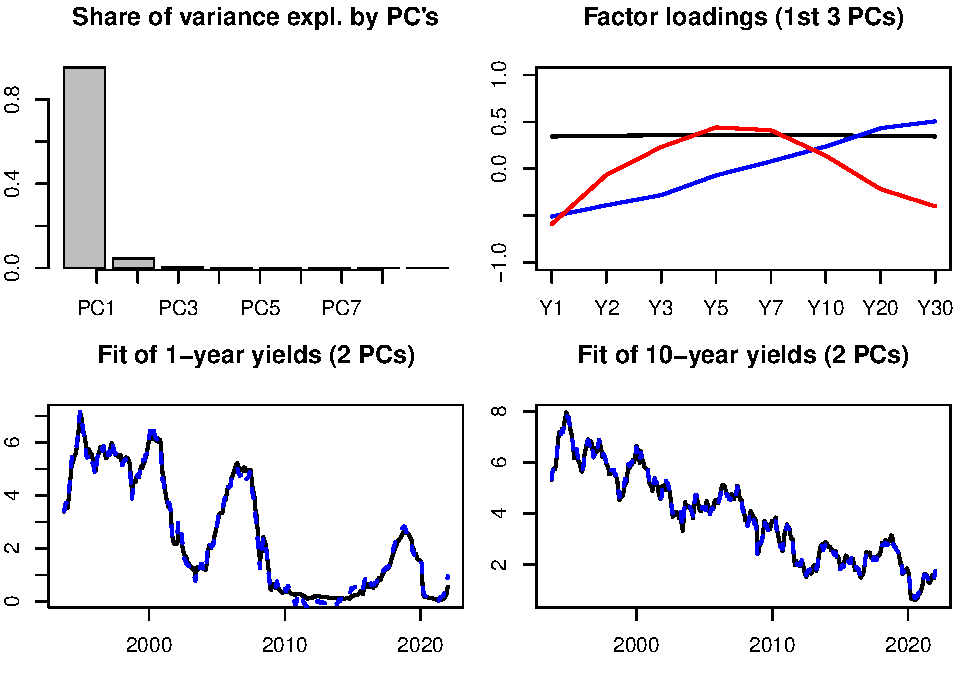
\includegraphics{IdentifStructShocks_files/figure-latex/USydsPCA1-1} \caption{Some PCA results. The dataset contains 8 time series of U.S. interest rates of different maturities.}\label{fig:USydsPCA1}
\end{figure}

\section{FAVAR models}\label{favar-models}

Let us denote by \(F_t\) a \(k\)-dimensional vector of latent factors accounting for important shares of the variances of the \(y_{i,t}\)'s (with \(K \ll n\)) and by \(x_t\) is a small \(M\)-dimensional subset of \(y_t\) (with \(M \ll n\)). The following factor structure is posited:
\[
y_t = \Lambda^f F_t + \Lambda^x x_t + e_t,
\]
where the \(e_t\) are ``small'' serially and mutually i.i.d. error terms. That is \(F_t\) and \(x_t\) are supposed to drive most of the fluctuations of \(y_t\)'s components.

The model is complemented by positing a VAR dynamics for \([F_t',x_t']'\):
\begin{equation}
\left[\begin{array}{c}F_t\\x_t\end{array}\right] = \Phi(L)\left[\begin{array}{c}F_{t-1}\\ x_{t-1}\end{array}\right] + v_t.\label{eq:FAVAR}
\end{equation}

Standard identification techniques of structural shocks can be employed in Eq. \eqref{eq:FAVAR}: Cholesky approach can be used for instance if the last component of \(x_t\) is the short-term interest rate and if it is assumed that a MP shock has no contemporaneous impact on other variables.

In their identification procedure, \citet{Bernanke_Boivin_Eliasz_2005} exploit the fact that macro-finance variables can be decomposed in two sets---fast-moving and slow-moving variables---and that only the former reacts contemporaneously to monetary-policy shocks. Now, how to estimate the (unobserved) factors \(F_t\)? \citet{Bernanke_Boivin_Eliasz_2005} note that the first \(K+M\) PCA of the whole dataset (\(y_t\)), that they denote by \(\hat{C}(F_t,x_t)\) should span the same space as \(F_t\) and \(x_t\). To get an estimate of \(F_t\), the dependence of \(\hat{C}(F_t,x_t)\) in \(x_t\) has to be removed. This is done by regressing, by OLS, \(\hat{C}(F_t,x_t)\) on \(x_t\) and on \(\hat{C}^*(F_t)\), where the latter is an estimate of the common components other than \(x_t\). To proxy for \(\hat{C}^*(F_t)\), \citet{Bernanke_Boivin_Eliasz_2005} take principal components from the set of slow-moving variables, that are not comtemporaneously correlated to \(x_t\). Vector \(\hat{F}_t\) is then computed as \(\hat{C}(F_t,x_t) - b_x x_t\), where \(b_x\) are the coefficients coming from the previous OLS regressions.

Note that this approach implies that the vectorial space spanned by \((\hat{F}_t,x_t)\) is the same as that spanned by \(\hat{C}(F_t,x_t)\).

Below, we employ this method on the dataset built by \citet{McCracken_Ng_2016} ---the \href{https://research.stlouisfed.org/wp/more/2015-012}{FRED:MD} database--- that includes 119 time series.

\begin{Shaded}
\begin{Highlighting}[]
\FunctionTok{library}\NormalTok{(BVAR)}\CommentTok{\# contains the fred\_md dataset}
\FunctionTok{library}\NormalTok{(IdSS)}
\FunctionTok{library}\NormalTok{(vars)}
\NormalTok{data }\OtherTok{\textless{}{-}} \FunctionTok{fred\_transform}\NormalTok{(fred\_md,}\AttributeTok{na.rm =} \ConstantTok{FALSE}\NormalTok{, }\AttributeTok{type =} \StringTok{"fred\_md"}\NormalTok{)}
\NormalTok{data }\OtherTok{\textless{}{-}}\NormalTok{ data[}\FunctionTok{complete.cases}\NormalTok{(data),]}
\NormalTok{data.values }\OtherTok{\textless{}{-}} \FunctionTok{scale}\NormalTok{(data, }\AttributeTok{center =} \ConstantTok{TRUE}\NormalTok{, }\AttributeTok{scale =} \ConstantTok{TRUE}\NormalTok{)}
\NormalTok{data\_scaled }\OtherTok{\textless{}{-}}\NormalTok{ data}
\NormalTok{data\_scaled[}\DecValTok{1}\SpecialCharTok{:}\FunctionTok{dim}\NormalTok{(data)[}\DecValTok{1}\NormalTok{],}\DecValTok{1}\SpecialCharTok{:}\FunctionTok{dim}\NormalTok{(data)[}\DecValTok{2}\NormalTok{]] }\OtherTok{\textless{}{-}}\NormalTok{ data.values}
\NormalTok{K }\OtherTok{\textless{}{-}} \DecValTok{3}
\NormalTok{M }\OtherTok{\textless{}{-}} \DecValTok{1}
\NormalTok{PCA }\OtherTok{\textless{}{-}} \FunctionTok{prcomp}\NormalTok{(data\_scaled) }\CommentTok{\# implies that PCA$x \%*\% t(PCA$rotation) = data}
\NormalTok{C.hat }\OtherTok{\textless{}{-}}\NormalTok{ PCA}\SpecialCharTok{$}\NormalTok{x[,}\DecValTok{1}\SpecialCharTok{:}\NormalTok{(K}\SpecialCharTok{+}\NormalTok{M)]}
\NormalTok{fast\_moving }\OtherTok{\textless{}{-}} \FunctionTok{c}\NormalTok{(}\StringTok{"HOUST"}\NormalTok{,}\StringTok{"HOUSTNE"}\NormalTok{,}\StringTok{"HOUSTMW"}\NormalTok{,}\StringTok{"HOUSTS"}\NormalTok{,}\StringTok{"HOUSTW"}\NormalTok{,}\StringTok{"HOUSTS"}\NormalTok{,}\StringTok{"AMDMNOx"}\NormalTok{,}
                 \StringTok{"FEDFUNDS"}\NormalTok{,}\StringTok{"CP3Mx"}\NormalTok{,}\StringTok{"TB3MS"}\NormalTok{,}\StringTok{"TB6MS"}\NormalTok{,}\StringTok{"GS1"}\NormalTok{,}\StringTok{"GS5"}\NormalTok{,}\StringTok{"GS10"}\NormalTok{,}
                 \StringTok{"COMPAPFFx"}\NormalTok{,}\StringTok{"TB3SMFFM"}\NormalTok{,}\StringTok{"TB6SMFFM"}\NormalTok{,}\StringTok{"T1YFFM"}\NormalTok{,}\StringTok{"T5YFFM"}\NormalTok{,}\StringTok{"T10YFFM"}\NormalTok{,}
                 \StringTok{"AAAFFM"}\NormalTok{,}\StringTok{"EXSZUSx"}\NormalTok{,}\StringTok{"EXJPUSx"}\NormalTok{,}\StringTok{"EXUSUKx"}\NormalTok{,}\StringTok{"EXCAUSx"}\NormalTok{)}
\NormalTok{data.slow }\OtherTok{\textless{}{-}}\NormalTok{ data\_scaled[,}\SpecialCharTok{{-}}\FunctionTok{which}\NormalTok{(fast\_moving }\SpecialCharTok{\%in\%} \FunctionTok{names}\NormalTok{(data))]}
\NormalTok{PCA.star }\OtherTok{\textless{}{-}} \FunctionTok{prcomp}\NormalTok{(data.slow) }\CommentTok{\# implies that PCA$x \%*\% t(PCA$rotation) = data}
\NormalTok{C.hat.star }\OtherTok{\textless{}{-}}\NormalTok{ PCA.star}\SpecialCharTok{$}\NormalTok{x[,}\DecValTok{1}\SpecialCharTok{:}\NormalTok{K]}
\NormalTok{D }\OtherTok{\textless{}{-}} \FunctionTok{cbind}\NormalTok{(data}\SpecialCharTok{$}\NormalTok{FEDFUNDS,C.hat.star)}
\NormalTok{b.x }\OtherTok{\textless{}{-}} \FunctionTok{solve}\NormalTok{(}\FunctionTok{t}\NormalTok{(D)}\SpecialCharTok{\%*\%}\NormalTok{D) }\SpecialCharTok{\%*\%} \FunctionTok{t}\NormalTok{(D) }\SpecialCharTok{\%*\%}\NormalTok{ C.hat}
\NormalTok{F.hat }\OtherTok{\textless{}{-}}\NormalTok{ C.hat }\SpecialCharTok{{-}}\NormalTok{ data}\SpecialCharTok{$}\NormalTok{FEDFUNDS }\SpecialCharTok{\%*\%} \FunctionTok{matrix}\NormalTok{(b.x[}\DecValTok{1}\NormalTok{,],}\AttributeTok{nrow=}\DecValTok{1}\NormalTok{)}
\NormalTok{data\_var }\OtherTok{\textless{}{-}} \FunctionTok{data.frame}\NormalTok{(F.hat, }\AttributeTok{FEDFUNDS =}\NormalTok{ data}\SpecialCharTok{$}\NormalTok{FEDFUNDS)}
\NormalTok{p }\OtherTok{\textless{}{-}} \DecValTok{10}
\NormalTok{var }\OtherTok{\textless{}{-}} \FunctionTok{VAR}\NormalTok{(data\_var, p)}
\NormalTok{Omega }\OtherTok{\textless{}{-}} \FunctionTok{var}\NormalTok{(}\FunctionTok{residuals}\NormalTok{(var))}
\NormalTok{B }\OtherTok{\textless{}{-}} \FunctionTok{t}\NormalTok{(}\FunctionTok{chol}\NormalTok{(Omega))}
\NormalTok{D }\OtherTok{\textless{}{-}} \FunctionTok{cbind}\NormalTok{(F.hat,data}\SpecialCharTok{$}\NormalTok{FEDFUNDS)}
\NormalTok{loadings }\OtherTok{\textless{}{-}} \FunctionTok{solve}\NormalTok{(}\FunctionTok{t}\NormalTok{(D)}\SpecialCharTok{\%*\%}\NormalTok{D) }\SpecialCharTok{\%*\%} \FunctionTok{t}\NormalTok{(D) }\SpecialCharTok{\%*\%} \FunctionTok{as.matrix}\NormalTok{(data\_scaled)}
\NormalTok{irf }\OtherTok{\textless{}{-}} \FunctionTok{simul.VAR}\NormalTok{(}\AttributeTok{c=}\FunctionTok{rep}\NormalTok{(}\DecValTok{0}\NormalTok{,(K}\SpecialCharTok{+}\NormalTok{M)}\SpecialCharTok{*}\NormalTok{p),}\AttributeTok{Phi=}\FunctionTok{Acoef}\NormalTok{(var),B,}\AttributeTok{nb.sim=}\DecValTok{120}\NormalTok{,}
                 \AttributeTok{y0.star=}\FunctionTok{rep}\NormalTok{(}\DecValTok{0}\NormalTok{,(K}\SpecialCharTok{+}\NormalTok{M)}\SpecialCharTok{*}\NormalTok{p),}\AttributeTok{indic.IRF =} \DecValTok{1}\NormalTok{,}
                 \AttributeTok{u.shock =} \FunctionTok{c}\NormalTok{(}\FunctionTok{rep}\NormalTok{(}\DecValTok{0}\NormalTok{,K}\SpecialCharTok{+}\DecValTok{1}\NormalTok{),}\DecValTok{1}\NormalTok{))}
\NormalTok{irf.all }\OtherTok{\textless{}{-}}\NormalTok{ irf }\SpecialCharTok{\%*\%}\NormalTok{ loadings}
\FunctionTok{par}\NormalTok{(}\AttributeTok{mfrow=}\FunctionTok{c}\NormalTok{(}\DecValTok{2}\NormalTok{,}\DecValTok{2}\NormalTok{))}
\NormalTok{variables.}\FloatTok{2.}\NormalTok{plot }\OtherTok{\textless{}{-}} \FunctionTok{c}\NormalTok{(}\StringTok{"FEDFUNDS"}\NormalTok{,}\StringTok{"INDPRO"}\NormalTok{,}\StringTok{"UNRATE"}\NormalTok{,}\StringTok{"CPIAUCSL"}\NormalTok{)}
\FunctionTok{par}\NormalTok{(}\AttributeTok{plt=}\FunctionTok{c}\NormalTok{(.}\DecValTok{2}\NormalTok{,.}\DecValTok{95}\NormalTok{,.}\DecValTok{3}\NormalTok{,.}\DecValTok{95}\NormalTok{))}
\ControlFlowTok{for}\NormalTok{(i }\ControlFlowTok{in} \DecValTok{1}\SpecialCharTok{:}\FunctionTok{length}\NormalTok{(variables.}\FloatTok{2.}\NormalTok{plot))\{}
  \FunctionTok{plot}\NormalTok{(}\FunctionTok{cumsum}\NormalTok{(irf.all[,}\FunctionTok{which}\NormalTok{(variables.}\FloatTok{2.}\NormalTok{plot[i]}\SpecialCharTok{==}\FunctionTok{names}\NormalTok{(data))]),}\AttributeTok{lwd=}\DecValTok{2}\NormalTok{,}
       \AttributeTok{type=}\StringTok{"l"}\NormalTok{,}\AttributeTok{xlab=}\StringTok{"months after shock"}\NormalTok{,}\AttributeTok{ylab=}\NormalTok{variables.}\FloatTok{2.}\NormalTok{plot[i])}
\NormalTok{\}}
\end{Highlighting}
\end{Shaded}

\begin{figure}
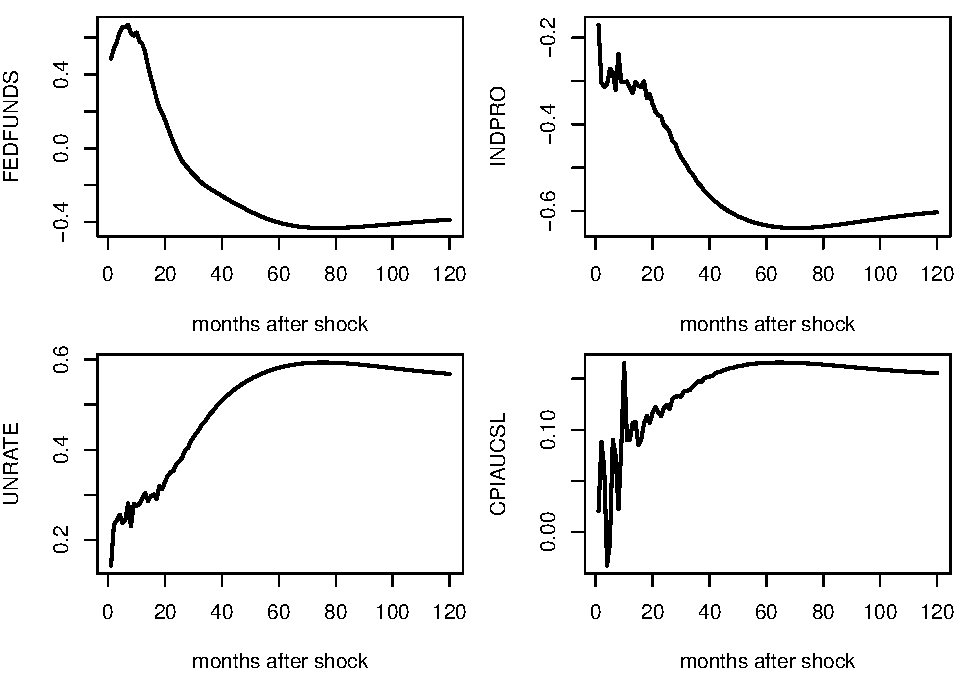
\includegraphics[width=0.95\linewidth]{IdentifStructShocks_files/figure-latex/FAVAR-1} \caption{Responses of a monetary-policy shock. FAVAR approach of Bernanke, Boivin, and Eliasz (2005). FRED-MD dataset.}\label{fig:FAVAR}
\end{figure}

\chapter{Appendix}\label{append}

\section{Definitions and statistical results}\label{definitions-and-statistical-results}

\begin{definition}[Covariance stationarity]
\protect\hypertarget{def:covstat}{}\label{def:covstat}The process \(y_t\) is covariance stationary ---or weakly stationary--- if, for all \(t\) and \(j\),
\[
\mathbb{E}(y_t) = \mu \quad \mbox{and} \quad \mathbb{E}\{(y_t - \mu)(y_{t-j} - \mu)\} = \gamma_j.
\]
\end{definition}

\begin{definition}[Likelihood Ratio test statistics]
\protect\hypertarget{def:LR}{}\label{def:LR}The likelihood ratio associated to a restriction of the form \(H_0: h({\boldsymbol\theta})=0\) (where \(h({\boldsymbol\theta})\) is a \(r\)-dimensional vector) is given by:
\[
LR = \frac{\mathcal{L}_R(\boldsymbol\theta;\mathbf{y})}{\mathcal{L}_U(\boldsymbol\theta;\mathbf{y})} \quad (\in [0,1]),
\]
where \(\mathcal{L}_R\) (respectively \(\mathcal{L}_U\)) is the likelihood function that imposes (resp. that does not impose) the restriction. The likelihood ratio test statistic is given by \(-2\log(LR)\), that is:
\[
\boxed{\xi^{LR}= 2 (\log\mathcal{L}_U(\boldsymbol\theta;\mathbf{y})-\log\mathcal{L}_R(\boldsymbol\theta;\mathbf{y})).}
\]
Under regularity assumptions and under the null hypothesis, the test statistic follows a chi-square distribution with \(r\) degrees of freedom (see Table \ref{tab:Chi2}).
\end{definition}

\begin{proposition}[p.d.f. of a multivariate Gaussian variable]
\protect\hypertarget{prp:pdfMultivarGaussian}{}\label{prp:pdfMultivarGaussian}If \(Y \sim \mathcal{N}(\mu,\Omega)\) and if \(Y\) is a \(n\)-dimensional vector, then the density function of \(Y\) is:
\[
\frac{1}{(2 \pi)^{n/2}|\Omega|^{1/2}}\exp\left[-\frac{1}{2}\left(Y-\mu\right)'\Omega^{-1}\left(Y-\mu\right)\right].
\]
\end{proposition}

\section{Estimation of VARMA models}\label{AppEstimVARMA}

Section \ref{estimVAR} discusses the estimation of VAR models and shows that standard VAR models can be esitmated by running OLS regressions.

If there is an MA component (i.e., if we consider a VARMA model), then OLS regressions yield biased estimates (even for asymptotically large samples). Assume for instance that \(y_t\) follows a VARMA(1,1) model:
\[
y_{i,t} = \phi_i y_{t-1} + \varepsilon_{i,t},
\]
where \(\phi_i\) is the \(i^{th}\) row of \(\Phi_1\), and where \(\varepsilon_{i,t}\) is a linear combination of \(\eta_t\) and \(\eta_{t-1}\). Since \(y_{t-1}\) (the regressor) is correlated to \(\eta_{t-1}\), it is also correlated to \(\varepsilon_{i,t}\). The OLS regression of \(y_{i,t}\) on \(y_{t-1}\) yields a biased estimator of \(\phi_i\) (see Figure \ref{fig:simulARMAbiased}). Hence, SVARMA models cannot be consistently estimated by simple OLS regressions (contrary to VAR models, as we will see in the next section); instrumental-variable approaches can be employed to estimate SVARMA models (using past values of \(y_t\) as instruments, see, e.g., \citet{Gourieroux_Monfort_Renne_2020}).

\begin{Shaded}
\begin{Highlighting}[]
\NormalTok{N }\OtherTok{\textless{}{-}} \DecValTok{1000} \CommentTok{\# number of replications}
\NormalTok{T }\OtherTok{\textless{}{-}} \DecValTok{100} \CommentTok{\# sample length}
\NormalTok{phi }\OtherTok{\textless{}{-}}\NormalTok{ .}\DecValTok{8} \CommentTok{\# autoregressive parameter}
\NormalTok{sigma }\OtherTok{\textless{}{-}} \DecValTok{1}
\FunctionTok{par}\NormalTok{(}\AttributeTok{mfrow=}\FunctionTok{c}\NormalTok{(}\DecValTok{1}\NormalTok{,}\DecValTok{2}\NormalTok{))}
\ControlFlowTok{for}\NormalTok{(theta }\ControlFlowTok{in} \FunctionTok{c}\NormalTok{(}\DecValTok{0}\NormalTok{,}\SpecialCharTok{{-}}\FloatTok{0.4}\NormalTok{))\{}
\NormalTok{  all.y }\OtherTok{\textless{}{-}} \FunctionTok{matrix}\NormalTok{(}\DecValTok{0}\NormalTok{,}\DecValTok{1}\NormalTok{,N)}
\NormalTok{  y     }\OtherTok{\textless{}{-}}\NormalTok{ all.y}
\NormalTok{  eta\_1 }\OtherTok{\textless{}{-}} \FunctionTok{rnorm}\NormalTok{(N)}
  \ControlFlowTok{for}\NormalTok{(t }\ControlFlowTok{in} \DecValTok{1}\SpecialCharTok{:}\NormalTok{(T}\SpecialCharTok{+}\DecValTok{1}\NormalTok{))\{}
\NormalTok{    eta }\OtherTok{\textless{}{-}} \FunctionTok{rnorm}\NormalTok{(N)}
\NormalTok{    y }\OtherTok{\textless{}{-}}\NormalTok{ phi }\SpecialCharTok{*}\NormalTok{ y }\SpecialCharTok{+}\NormalTok{ sigma }\SpecialCharTok{*}\NormalTok{ eta }\SpecialCharTok{+}\NormalTok{ theta }\SpecialCharTok{*}\NormalTok{ sigma }\SpecialCharTok{*}\NormalTok{ eta\_1}
\NormalTok{    all.y }\OtherTok{\textless{}{-}} \FunctionTok{rbind}\NormalTok{(all.y,y)}
\NormalTok{    eta\_1 }\OtherTok{\textless{}{-}}\NormalTok{ eta}
\NormalTok{  \}}
\NormalTok{  all.y\_1 }\OtherTok{\textless{}{-}}\NormalTok{ all.y[}\DecValTok{1}\SpecialCharTok{:}\NormalTok{T,]}
\NormalTok{  all.y   }\OtherTok{\textless{}{-}}\NormalTok{ all.y[}\DecValTok{2}\SpecialCharTok{:}\NormalTok{(T}\SpecialCharTok{+}\DecValTok{1}\NormalTok{),]}
\NormalTok{  XX\_1 }\OtherTok{\textless{}{-}} \DecValTok{1}\SpecialCharTok{/}\FunctionTok{apply}\NormalTok{(all.y\_1 }\SpecialCharTok{*}\NormalTok{ all.y\_1,}\DecValTok{2}\NormalTok{,sum)}
\NormalTok{  XY   }\OtherTok{\textless{}{-}} \FunctionTok{apply}\NormalTok{(all.y\_1 }\SpecialCharTok{*}\NormalTok{ all.y,}\DecValTok{2}\NormalTok{,sum)}
\NormalTok{  phi.est.OLS }\OtherTok{\textless{}{-}}\NormalTok{ XX\_1 }\SpecialCharTok{*}\NormalTok{ XY}
  \FunctionTok{plot}\NormalTok{(}\FunctionTok{density}\NormalTok{(phi.est.OLS),}\AttributeTok{xlab=}\StringTok{"OLS estimate of phi"}\NormalTok{,}\AttributeTok{ylab=}\StringTok{""}\NormalTok{,}
       \AttributeTok{main=}\FunctionTok{paste}\NormalTok{(}\StringTok{"theta = "}\NormalTok{,theta,}\AttributeTok{sep=}\StringTok{""}\NormalTok{))}
  \FunctionTok{abline}\NormalTok{(}\AttributeTok{v=}\NormalTok{phi,}\AttributeTok{col=}\StringTok{"red"}\NormalTok{,}\AttributeTok{lwd=}\DecValTok{2}\NormalTok{)\}}
\end{Highlighting}
\end{Shaded}

\begin{figure}
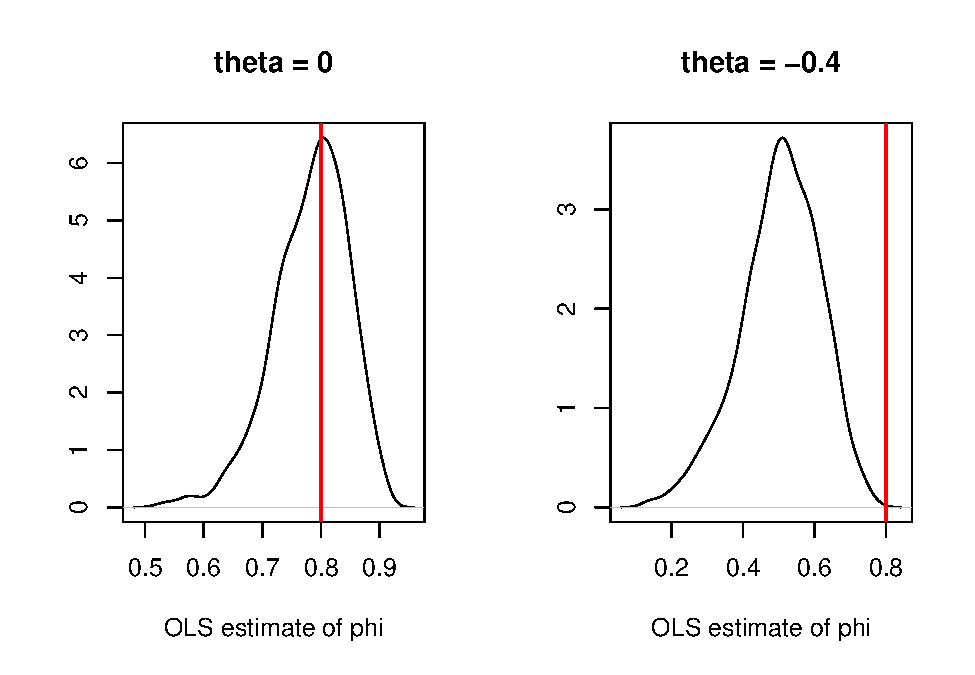
\includegraphics[width=0.95\linewidth]{IdentifStructShocks_files/figure-latex/simulARMAbiased-1} \caption{Illustration of the bias obtained when estimating the auto-regressive parameters of an ARMA process by (standard) OLS.}\label{fig:simulARMAbiased}
\end{figure}

\section{Proofs}\label{AppendixProof}

\textbf{Proof of Proposition \ref{prp:estimVARGaussian}}

\begin{proof}
Using Proposition \ref{prp:pdfMultivarGaussian}, we obtain that, conditionally on \(x_1\), the log-likelihood is given by
\begin{eqnarray*}
\log\mathcal{L}(Y_{T};\theta) & = & -(Tn/2)\log(2\pi)+(T/2)\log\left|\Omega^{-1}\right|\\
&  & -\frac{1}{2}\sum_{t=1}^{T}\left[\left(y_{t}-\Pi'x_{t}\right)'\Omega^{-1}\left(y_{t}-\Pi'x_{t}\right)\right].
\end{eqnarray*}
Let's rewrite the last term of the log-likelihood:
\begin{eqnarray*}
\sum_{t=1}^{T}\left[\left(y_{t}-\Pi'x_{t}\right)'\Omega^{-1}\left(y_{t}-\Pi'x_{t}\right)\right] & =\\
\sum_{t=1}^{T}\left[\left(y_{t}-\hat{\Pi}'x_{t}+\hat{\Pi}'x_{t}-\Pi'x_{t}\right)'\Omega^{-1}\left(y_{t}-\hat{\Pi}'x_{t}+\hat{\Pi}'x_{t}-\Pi'x_{t}\right)\right] & =\\
\sum_{t=1}^{T}\left[\left(\hat{\varepsilon}_{t}+(\hat{\Pi}-\Pi)'x_{t}\right)'\Omega^{-1}\left(\hat{\varepsilon}_{t}+(\hat{\Pi}-\Pi)'x_{t}\right)\right],
\end{eqnarray*}
where the \(j^{th}\) element of the \((n\times1)\) vector \(\hat{\varepsilon}_{t}\) is the sample residual, for observation \(t\), from an OLS regression of \(y_{j,t}\) on \(x_{t}\). Expanding the previous equation, we get:
\begin{eqnarray*}
&&\sum_{t=1}^{T}\left[\left(y_{t}-\Pi'x_{t}\right)'\Omega^{-1}\left(y_{t}-\Pi'x_{t}\right)\right]  = \sum_{t=1}^{T}\hat{\varepsilon}_{t}'\Omega^{-1}\hat{\varepsilon}_{t}\\
&&+2\sum_{t=1}^{T}\hat{\varepsilon}_{t}'\Omega^{-1}(\hat{\Pi}-\Pi)'x_{t}+\sum_{t=1}^{T}x'_{t}(\hat{\Pi}-\Pi)\Omega^{-1}(\hat{\Pi}-\Pi)'x_{t}.
\end{eqnarray*}
Let's apply the trace operator on the second term (that is a scalar):
\begin{eqnarray*}
\sum_{t=1}^{T}\hat{\varepsilon}_{t}'\Omega^{-1}(\hat{\Pi}-\Pi)'x_{t} & = & Tr\left(\sum_{t=1}^{T}\hat{\varepsilon}_{t}'\Omega^{-1}(\hat{\Pi}-\Pi)'x_{t}\right)\\
=  Tr\left(\sum_{t=1}^{T}\Omega^{-1}(\hat{\Pi}-\Pi)'x_{t}\hat{\varepsilon}_{t}'\right) & = & Tr\left(\Omega^{-1}(\hat{\Pi}-\Pi)'\sum_{t=1}^{T}x_{t}\hat{\varepsilon}_{t}'\right).
\end{eqnarray*}
Given that, by construction (property of OLS estimates), the sample residuals are orthogonal to the explanatory variables, this term is zero. Introducing \(\tilde{x}_{t}=(\hat{\Pi}-\Pi)'x_{t}\), we have
\begin{eqnarray*}
\sum_{t=1}^{T}\left[\left(y_{t}-\Pi'x_{t}\right)'\Omega^{-1}\left(y_{t}-\Pi'x_{t}\right)\right] =\sum_{t=1}^{T}\hat{\varepsilon}_{t}'\Omega^{-1}\hat{\varepsilon}_{t}+\sum_{t=1}^{T}\tilde{x}'_{t}\Omega^{-1}\tilde{x}_{t}.
\end{eqnarray*}
Since \(\Omega\) is a positive definite matrix, \(\Omega^{-1}\) is as well. Consequently, the smallest value that the last term can take is obtained for \(\tilde{x}_{t}=0\), i.e.~when \(\Pi=\hat{\Pi}.\)

The MLE of \(\Omega\) is the matrix \(\hat{\Omega}\) that maximizes \(\Omega\overset{\ell}{\rightarrow}L(Y_{T};\hat{\Pi},\Omega)\). We have:
\begin{eqnarray*}
\log\mathcal{L}(Y_{T};\hat{\Pi},\Omega) & = & -(Tn/2)\log(2\pi)+(T/2)\log\left|\Omega^{-1}\right| -\frac{1}{2}\sum_{t=1}^{T}\left[\hat{\varepsilon}_{t}'\Omega^{-1}\hat{\varepsilon}_{t}\right].
\end{eqnarray*}

Matrix \(\hat{\Omega}\) is a symmetric positive definite. It is easily checked that the (unrestricted) matrix that maximizes the latter expression is symmetric positive definite matrix. Indeed:
\[
\frac{\partial \log\mathcal{L}(Y_{T};\hat{\Pi},\Omega)}{\partial\Omega}=\frac{T}{2}\Omega'-\frac{1}{2}\sum_{t=1}^{T}\hat{\varepsilon}_{t}\hat{\varepsilon}'_{t}\Rightarrow\hat{\Omega}'=\frac{1}{T}\sum_{t=1}^{T}\hat{\varepsilon}_{t}\hat{\varepsilon}'_{t},
\]
which leads to the result.
\end{proof}

\textbf{Proof of Proposition \ref{prp:OLSVAR}}

\begin{proof}
Let us drop the \(i\) subscript. Rearranging Eq. \eqref{eq:olsar1}, we have:
\[
\sqrt{T}(\mathbf{b}-\boldsymbol{\beta}) =  (X'X/T)^{-1}\sqrt{T}(X'\boldsymbol\varepsilon/T).
\]
Let us consider the autocovariances of \(\mathbf{v}_t = x_t \varepsilon_t\), denoted by \(\gamma^v_j\). Using the fact that \(x_t\) is a linear combination of past \(\varepsilon_t\)s and that \(\varepsilon_t\) is a white noise, we get that \(\mathbb{E}(\varepsilon_t x_t)=0\). Therefore
\[
\gamma^v_j = \mathbb{E}(\varepsilon_t\varepsilon_{t-j}x_tx_{t-j}').
\]
If \(j>0\), we have \(\mathbb{E}(\varepsilon_t\varepsilon_{t-j}x_tx_{t-j}')=\mathbb{E}(\mathbb{E}[\varepsilon_t\varepsilon_{t-j}x_tx_{t-j}'|\varepsilon_{t-j},x_t,x_{t-j}])=\) \(\mathbb{E}(\varepsilon_{t-j}x_tx_{t-j}'\mathbb{E}[\varepsilon_t|\varepsilon_{t-j},x_t,x_{t-j}])=0\). Note that we have \(\mathbb{E}[\varepsilon_t|\varepsilon_{t-j},x_t,x_{t-j}]=0\) because \(\{\varepsilon_t\}\) is an i.i.d. white noise sequence. If \(j=0\), we have:
\[
\gamma^v_0 = \mathbb{E}(\varepsilon_t^2x_tx_{t}')= \mathbb{E}(\varepsilon_t^2) \mathbb{E}(x_tx_{t}')=\sigma^2\mathbf{Q}.
\]
The convergence in distribution of \(\sqrt{T}(X'\boldsymbol\varepsilon/T)=\sqrt{T}\frac{1}{T}\sum_{t=1}^Tv_t\) results from the Central Limit Theorem for covariance-stationary processes, using the \(\gamma_j^v\) computed above.
\end{proof}

\section{Statistical Tables}\label{statistical-tables}

\begin{table}

\caption{\label{tab:Normal}Quantiles of the $\mathcal{N}(0,1)$ distribution. If $a$ and $b$ are respectively the row and column number; then the corresponding cell gives $\mathbb{P}(0<X\le a+b)$, where $X \sim \mathcal{N}(0,1)$.}
\centering
\begin{tabular}[t]{l|r|r|r|r|r|r|r|r|r|r}
\hline
  & 0 & 0.01 & 0.02 & 0.03 & 0.04 & 0.05 & 0.06 & 0.07 & 0.08 & 0.09\\
\hline
0 & 0.5000 & 0.6179 & 0.7257 & 0.8159 & 0.8849 & 0.9332 & 0.9641 & 0.9821 & 0.9918 & 0.9965\\
\hline
0.1 & 0.5040 & 0.6217 & 0.7291 & 0.8186 & 0.8869 & 0.9345 & 0.9649 & 0.9826 & 0.9920 & 0.9966\\
\hline
0.2 & 0.5080 & 0.6255 & 0.7324 & 0.8212 & 0.8888 & 0.9357 & 0.9656 & 0.9830 & 0.9922 & 0.9967\\
\hline
0.3 & 0.5120 & 0.6293 & 0.7357 & 0.8238 & 0.8907 & 0.9370 & 0.9664 & 0.9834 & 0.9925 & 0.9968\\
\hline
0.4 & 0.5160 & 0.6331 & 0.7389 & 0.8264 & 0.8925 & 0.9382 & 0.9671 & 0.9838 & 0.9927 & 0.9969\\
\hline
0.5 & 0.5199 & 0.6368 & 0.7422 & 0.8289 & 0.8944 & 0.9394 & 0.9678 & 0.9842 & 0.9929 & 0.9970\\
\hline
0.6 & 0.5239 & 0.6406 & 0.7454 & 0.8315 & 0.8962 & 0.9406 & 0.9686 & 0.9846 & 0.9931 & 0.9971\\
\hline
0.7 & 0.5279 & 0.6443 & 0.7486 & 0.8340 & 0.8980 & 0.9418 & 0.9693 & 0.9850 & 0.9932 & 0.9972\\
\hline
0.8 & 0.5319 & 0.6480 & 0.7517 & 0.8365 & 0.8997 & 0.9429 & 0.9699 & 0.9854 & 0.9934 & 0.9973\\
\hline
0.9 & 0.5359 & 0.6517 & 0.7549 & 0.8389 & 0.9015 & 0.9441 & 0.9706 & 0.9857 & 0.9936 & 0.9974\\
\hline
1 & 0.5398 & 0.6554 & 0.7580 & 0.8413 & 0.9032 & 0.9452 & 0.9713 & 0.9861 & 0.9938 & 0.9974\\
\hline
1.1 & 0.5438 & 0.6591 & 0.7611 & 0.8438 & 0.9049 & 0.9463 & 0.9719 & 0.9864 & 0.9940 & 0.9975\\
\hline
1.2 & 0.5478 & 0.6628 & 0.7642 & 0.8461 & 0.9066 & 0.9474 & 0.9726 & 0.9868 & 0.9941 & 0.9976\\
\hline
1.3 & 0.5517 & 0.6664 & 0.7673 & 0.8485 & 0.9082 & 0.9484 & 0.9732 & 0.9871 & 0.9943 & 0.9977\\
\hline
1.4 & 0.5557 & 0.6700 & 0.7704 & 0.8508 & 0.9099 & 0.9495 & 0.9738 & 0.9875 & 0.9945 & 0.9977\\
\hline
1.5 & 0.5596 & 0.6736 & 0.7734 & 0.8531 & 0.9115 & 0.9505 & 0.9744 & 0.9878 & 0.9946 & 0.9978\\
\hline
1.6 & 0.5636 & 0.6772 & 0.7764 & 0.8554 & 0.9131 & 0.9515 & 0.9750 & 0.9881 & 0.9948 & 0.9979\\
\hline
1.7 & 0.5675 & 0.6808 & 0.7794 & 0.8577 & 0.9147 & 0.9525 & 0.9756 & 0.9884 & 0.9949 & 0.9979\\
\hline
1.8 & 0.5714 & 0.6844 & 0.7823 & 0.8599 & 0.9162 & 0.9535 & 0.9761 & 0.9887 & 0.9951 & 0.9980\\
\hline
1.9 & 0.5753 & 0.6879 & 0.7852 & 0.8621 & 0.9177 & 0.9545 & 0.9767 & 0.9890 & 0.9952 & 0.9981\\
\hline
2 & 0.5793 & 0.6915 & 0.7881 & 0.8643 & 0.9192 & 0.9554 & 0.9772 & 0.9893 & 0.9953 & 0.9981\\
\hline
2.1 & 0.5832 & 0.6950 & 0.7910 & 0.8665 & 0.9207 & 0.9564 & 0.9778 & 0.9896 & 0.9955 & 0.9982\\
\hline
2.2 & 0.5871 & 0.6985 & 0.7939 & 0.8686 & 0.9222 & 0.9573 & 0.9783 & 0.9898 & 0.9956 & 0.9982\\
\hline
2.3 & 0.5910 & 0.7019 & 0.7967 & 0.8708 & 0.9236 & 0.9582 & 0.9788 & 0.9901 & 0.9957 & 0.9983\\
\hline
2.4 & 0.5948 & 0.7054 & 0.7995 & 0.8729 & 0.9251 & 0.9591 & 0.9793 & 0.9904 & 0.9959 & 0.9984\\
\hline
2.5 & 0.5987 & 0.7088 & 0.8023 & 0.8749 & 0.9265 & 0.9599 & 0.9798 & 0.9906 & 0.9960 & 0.9984\\
\hline
2.6 & 0.6026 & 0.7123 & 0.8051 & 0.8770 & 0.9279 & 0.9608 & 0.9803 & 0.9909 & 0.9961 & 0.9985\\
\hline
2.7 & 0.6064 & 0.7157 & 0.8078 & 0.8790 & 0.9292 & 0.9616 & 0.9808 & 0.9911 & 0.9962 & 0.9985\\
\hline
2.8 & 0.6103 & 0.7190 & 0.8106 & 0.8810 & 0.9306 & 0.9625 & 0.9812 & 0.9913 & 0.9963 & 0.9986\\
\hline
2.9 & 0.6141 & 0.7224 & 0.8133 & 0.8830 & 0.9319 & 0.9633 & 0.9817 & 0.9916 & 0.9964 & 0.9986\\
\hline
\end{tabular}
\end{table}

\begin{table}

\caption{\label{tab:Student}Quantiles of the Student-$t$ distribution. The rows correspond to different degrees of freedom ($\nu$, say); the columns correspond to different probabilities ($z$, say). The cell gives $q$ that is s.t. $\mathbb{P}(-q<X<q)=z$, with $X \sim t(\nu)$.}
\centering
\begin{tabular}[t]{l|r|r|r|r|r|r|r|r}
\hline
  & 0.05 & 0.1 & 0.75 & 0.9 & 0.95 & 0.975 & 0.99 & 0.999\\
\hline
1 & 0.079 & 0.158 & 2.414 & 6.314 & 12.706 & 25.452 & 63.657 & 636.619\\
\hline
2 & 0.071 & 0.142 & 1.604 & 2.920 & 4.303 & 6.205 & 9.925 & 31.599\\
\hline
3 & 0.068 & 0.137 & 1.423 & 2.353 & 3.182 & 4.177 & 5.841 & 12.924\\
\hline
4 & 0.067 & 0.134 & 1.344 & 2.132 & 2.776 & 3.495 & 4.604 & 8.610\\
\hline
5 & 0.066 & 0.132 & 1.301 & 2.015 & 2.571 & 3.163 & 4.032 & 6.869\\
\hline
6 & 0.065 & 0.131 & 1.273 & 1.943 & 2.447 & 2.969 & 3.707 & 5.959\\
\hline
7 & 0.065 & 0.130 & 1.254 & 1.895 & 2.365 & 2.841 & 3.499 & 5.408\\
\hline
8 & 0.065 & 0.130 & 1.240 & 1.860 & 2.306 & 2.752 & 3.355 & 5.041\\
\hline
9 & 0.064 & 0.129 & 1.230 & 1.833 & 2.262 & 2.685 & 3.250 & 4.781\\
\hline
10 & 0.064 & 0.129 & 1.221 & 1.812 & 2.228 & 2.634 & 3.169 & 4.587\\
\hline
20 & 0.063 & 0.127 & 1.185 & 1.725 & 2.086 & 2.423 & 2.845 & 3.850\\
\hline
30 & 0.063 & 0.127 & 1.173 & 1.697 & 2.042 & 2.360 & 2.750 & 3.646\\
\hline
40 & 0.063 & 0.126 & 1.167 & 1.684 & 2.021 & 2.329 & 2.704 & 3.551\\
\hline
50 & 0.063 & 0.126 & 1.164 & 1.676 & 2.009 & 2.311 & 2.678 & 3.496\\
\hline
60 & 0.063 & 0.126 & 1.162 & 1.671 & 2.000 & 2.299 & 2.660 & 3.460\\
\hline
70 & 0.063 & 0.126 & 1.160 & 1.667 & 1.994 & 2.291 & 2.648 & 3.435\\
\hline
80 & 0.063 & 0.126 & 1.159 & 1.664 & 1.990 & 2.284 & 2.639 & 3.416\\
\hline
90 & 0.063 & 0.126 & 1.158 & 1.662 & 1.987 & 2.280 & 2.632 & 3.402\\
\hline
100 & 0.063 & 0.126 & 1.157 & 1.660 & 1.984 & 2.276 & 2.626 & 3.390\\
\hline
200 & 0.063 & 0.126 & 1.154 & 1.653 & 1.972 & 2.258 & 2.601 & 3.340\\
\hline
500 & 0.063 & 0.126 & 1.152 & 1.648 & 1.965 & 2.248 & 2.586 & 3.310\\
\hline
\end{tabular}
\end{table}

\begin{table}

\caption{\label{tab:Chi2}Quantiles of the $\chi^2$ distribution. The rows correspond to different degrees of freedom; the columns correspond to different probabilities.}
\centering
\begin{tabular}[t]{l|r|r|r|r|r|r|r|r}
\hline
  & 0.05 & 0.1 & 0.75 & 0.9 & 0.95 & 0.975 & 0.99 & 0.999\\
\hline
1 & 0.004 & 0.016 & 1.323 & 2.706 & 3.841 & 5.024 & 6.635 & 10.828\\
\hline
2 & 0.103 & 0.211 & 2.773 & 4.605 & 5.991 & 7.378 & 9.210 & 13.816\\
\hline
3 & 0.352 & 0.584 & 4.108 & 6.251 & 7.815 & 9.348 & 11.345 & 16.266\\
\hline
4 & 0.711 & 1.064 & 5.385 & 7.779 & 9.488 & 11.143 & 13.277 & 18.467\\
\hline
5 & 1.145 & 1.610 & 6.626 & 9.236 & 11.070 & 12.833 & 15.086 & 20.515\\
\hline
6 & 1.635 & 2.204 & 7.841 & 10.645 & 12.592 & 14.449 & 16.812 & 22.458\\
\hline
7 & 2.167 & 2.833 & 9.037 & 12.017 & 14.067 & 16.013 & 18.475 & 24.322\\
\hline
8 & 2.733 & 3.490 & 10.219 & 13.362 & 15.507 & 17.535 & 20.090 & 26.124\\
\hline
9 & 3.325 & 4.168 & 11.389 & 14.684 & 16.919 & 19.023 & 21.666 & 27.877\\
\hline
10 & 3.940 & 4.865 & 12.549 & 15.987 & 18.307 & 20.483 & 23.209 & 29.588\\
\hline
20 & 10.851 & 12.443 & 23.828 & 28.412 & 31.410 & 34.170 & 37.566 & 45.315\\
\hline
30 & 18.493 & 20.599 & 34.800 & 40.256 & 43.773 & 46.979 & 50.892 & 59.703\\
\hline
40 & 26.509 & 29.051 & 45.616 & 51.805 & 55.758 & 59.342 & 63.691 & 73.402\\
\hline
50 & 34.764 & 37.689 & 56.334 & 63.167 & 67.505 & 71.420 & 76.154 & 86.661\\
\hline
60 & 43.188 & 46.459 & 66.981 & 74.397 & 79.082 & 83.298 & 88.379 & 99.607\\
\hline
70 & 51.739 & 55.329 & 77.577 & 85.527 & 90.531 & 95.023 & 100.425 & 112.317\\
\hline
80 & 60.391 & 64.278 & 88.130 & 96.578 & 101.879 & 106.629 & 112.329 & 124.839\\
\hline
90 & 69.126 & 73.291 & 98.650 & 107.565 & 113.145 & 118.136 & 124.116 & 137.208\\
\hline
100 & 77.929 & 82.358 & 109.141 & 118.498 & 124.342 & 129.561 & 135.807 & 149.449\\
\hline
200 & 168.279 & 174.835 & 213.102 & 226.021 & 233.994 & 241.058 & 249.445 & 267.541\\
\hline
500 & 449.147 & 459.926 & 520.950 & 540.930 & 553.127 & 563.852 & 576.493 & 603.446\\
\hline
\end{tabular}
\end{table}

\begin{table}

\caption{\label{tab:Fstat}Quantiles of the $\mathcal{F}$ distribution. The columns and rows correspond to different degrees of freedom (resp. $n_1$ and $n_2$). The different panels correspond to different probabilities ($\alpha$) The corresponding cell gives $z$ that is s.t. $\mathbb{P}(X \le z)=\alpha$, with $X \sim \mathcal{F}(n_1,n_2)$.}
\centering
\begin{tabular}[t]{l|r|r|r|r|r|r|r|r|r|r}
\hline
  & 1 & 2 & 3 & 4 & 5 & 6 & 7 & 8 & 9 & 10\\
\hline
alpha = 0.9 &  &  &  &  &  &  &  &  &  & \\
\hline
5 & 4.060 & 3.780 & 3.619 & 3.520 & 3.453 & 3.405 & 3.368 & 3.339 & 3.316 & 3.297\\
\hline
10 & 3.285 & 2.924 & 2.728 & 2.605 & 2.522 & 2.461 & 2.414 & 2.377 & 2.347 & 2.323\\
\hline
15 & 3.073 & 2.695 & 2.490 & 2.361 & 2.273 & 2.208 & 2.158 & 2.119 & 2.086 & 2.059\\
\hline
20 & 2.975 & 2.589 & 2.380 & 2.249 & 2.158 & 2.091 & 2.040 & 1.999 & 1.965 & 1.937\\
\hline
50 & 2.809 & 2.412 & 2.197 & 2.061 & 1.966 & 1.895 & 1.840 & 1.796 & 1.760 & 1.729\\
\hline
100 & 2.756 & 2.356 & 2.139 & 2.002 & 1.906 & 1.834 & 1.778 & 1.732 & 1.695 & 1.663\\
\hline
500 & 2.716 & 2.313 & 2.095 & 1.956 & 1.859 & 1.786 & 1.729 & 1.683 & 1.644 & 1.612\\
\hline
alpha = 0.95 &  &  &  &  &  &  &  &  &  & \\
\hline
5 & 6.608 & 5.786 & 5.409 & 5.192 & 5.050 & 4.950 & 4.876 & 4.818 & 4.772 & 4.735\\
\hline
10 & 4.965 & 4.103 & 3.708 & 3.478 & 3.326 & 3.217 & 3.135 & 3.072 & 3.020 & 2.978\\
\hline
15 & 4.543 & 3.682 & 3.287 & 3.056 & 2.901 & 2.790 & 2.707 & 2.641 & 2.588 & 2.544\\
\hline
20 & 4.351 & 3.493 & 3.098 & 2.866 & 2.711 & 2.599 & 2.514 & 2.447 & 2.393 & 2.348\\
\hline
50 & 4.034 & 3.183 & 2.790 & 2.557 & 2.400 & 2.286 & 2.199 & 2.130 & 2.073 & 2.026\\
\hline
100 & 3.936 & 3.087 & 2.696 & 2.463 & 2.305 & 2.191 & 2.103 & 2.032 & 1.975 & 1.927\\
\hline
500 & 3.860 & 3.014 & 2.623 & 2.390 & 2.232 & 2.117 & 2.028 & 1.957 & 1.899 & 1.850\\
\hline
alpha = 0.99 &  &  &  &  &  &  &  &  &  & \\
\hline
5 & 16.258 & 13.274 & 12.060 & 11.392 & 10.967 & 10.672 & 10.456 & 10.289 & 10.158 & 10.051\\
\hline
10 & 10.044 & 7.559 & 6.552 & 5.994 & 5.636 & 5.386 & 5.200 & 5.057 & 4.942 & 4.849\\
\hline
15 & 8.683 & 6.359 & 5.417 & 4.893 & 4.556 & 4.318 & 4.142 & 4.004 & 3.895 & 3.805\\
\hline
20 & 8.096 & 5.849 & 4.938 & 4.431 & 4.103 & 3.871 & 3.699 & 3.564 & 3.457 & 3.368\\
\hline
50 & 7.171 & 5.057 & 4.199 & 3.720 & 3.408 & 3.186 & 3.020 & 2.890 & 2.785 & 2.698\\
\hline
100 & 6.895 & 4.824 & 3.984 & 3.513 & 3.206 & 2.988 & 2.823 & 2.694 & 2.590 & 2.503\\
\hline
500 & 6.686 & 4.648 & 3.821 & 3.357 & 3.054 & 2.838 & 2.675 & 2.547 & 2.443 & 2.356\\
\hline
\end{tabular}
\end{table}

  \bibliography{book.bib,packages.bib}

\end{document}
